\documentclass[10pt]{article}

\usepackage[pdftex]{graphicx} 
  \usepackage{pgfplots}
\pgfplotsset{compat=newest}
%% the following commands are needed for some matlab2tikz features
\usetikzlibrary{plotmarks}
\usetikzlibrary{arrows.meta}
\usepgfplotslibrary{patchplots}
\usepackage{grffile}
\usepackage{amsmath}


%\usepackage{fullpage}
\usepackage[top=1in, bottom=1in, left=0.8in, right=1in]{geometry}
\usepackage{multicol}
%\usepackage{wrapfig}
%\usepackage{listings}
\usepackage{caption}
\usepackage{subcaption}
\usepackage{hyperref}
\usepackage{xcolor}
%\usepackage{soul}
\usepackage{tikz}

\definecolor{lightblue}{rgb}{.80,.9,1}
\newcommand{\hl}[1]
    {\par\colorbox{lightblue}{\parbox{\linewidth}{#1}}}

\newcommand{\defn}{\stackrel{\textrm{\scriptsize def}}{=}}

\setlength{\columnsep}{0.1pc}

\title{gSGN Wave Speeds and The Dam-break Problem.}
%\author{Christopher Zoppou -- \texttt{christopher.zoppou@anu.edu.au}, Dimitrios Mitsotakis -- \texttt{dmitsot@gmail.com}, Stephen Roberts -- \texttt{stephen.roberts@anu.edu.au}, Jordan Pitt}

% TIME ON EVERY PAGE AS WELL AS THE FILE NAME
\usepackage{fancyhdr}
\usepackage{currfile}
\usepackage[us,12hr]{datetime} % `us' makes \today behave as usual in TeX/LaTeX
\fancypagestyle{plain}{
\fancyhf{}
\rfoot{\emph{\footnotesize \textcopyright  gSGN Letter to Dimitrios Mitsotakis by Jordan Pitt, Chris Zoppou and Stephen Roberts.}
 \\ File Name: {\currfilename} \\ Date: {\ddmmyyyydate\today} at \currenttime}
\lfoot{Page \thepage}
\renewcommand{\headrulewidth}{0pt}}
\pagestyle{plain}

\begin{document}

\maketitle

\vspace{-0.3in}
\noindent
\rule{\linewidth}{0.4pt}

%-------------------------------------------------
%\section{Introduction}
%-------------------------------------------------
Hello Dimitrios, I have adapted the $\text{FDVM}_2$ method in \cite{Zoppou-etal-2017} to solve the gSGN (generalised Serre-Green-Naghsi) equations from \cite{Clamond-Dutykh-2018-237}. 

The $\text{FDVM}_2$ method uses a second-order finite difference approximation to solve the elliptic equation that related the new conserved quantity $G$ to the primitive variable $u$, and a finite volume method with second-order Runge-Kutta time stepping to obtain a fully second order method. I have been able to demonstrate convergence to forced solutions and the ability of the method to reproduce the analytic solutions for well known members of this family of equations captureed by the gSGN; the dambreak problem for the SWWE and the soliton solution for the Serre equations.

To remind you, the gSGN equations and its reformulation into a conservative form are here.

%-------------------------------------------------
\section{gSGN - generalised Serre-Green-Naghdi equations}
%-------------------------------------------------
\cite{Clamond-Dutykh-2018-237} derived the following generalised version of the Serre-Green-Naghdi equations:

\begin{subequations}
	\begin{gather}
	\dfrac{\partial h}{\partial t} + \dfrac{\partial (uh)}{\partial x} = 0
	\label{eq:gSGNh}
	\end{gather}
	\begin{gather}
	\dfrac{\partial (uh)}{\partial t} + \dfrac{\partial }{\partial x} \left( u^2h + \dfrac{gh^2}{2} + \frac{1}{3} h^2 \Gamma \right)= 0
	\label{eq:gSGNuh}
	\end{gather}
	\begin{multline}
	\dfrac{\partial}{\partial t}\left[\frac{1}{2}hu^2 + \dfrac{1}{2}\left(1 + \frac{3}{2}\beta_1\right) h^3 \dfrac{\partial u}{\partial x}\dfrac{\partial u}{\partial x} + \frac{1}{2}gh^2\left(1 + \frac{1}{2}\beta_2 \dfrac{\partial h}{\partial x} \dfrac{\partial h}{\partial x}\right) \right] \\
	\dfrac{\partial}{\partial x}\left[uh\left(\frac{1}{2}u^2 + \dfrac{1}{2}\left(1 + \frac{3}{2}\beta_1\right)h^2\dfrac{\partial u}{\partial x}\dfrac{\partial u}{\partial x} + gh\left(1 + \frac{1}{4}\beta_2\dfrac{\partial h}{\partial x}\dfrac{\partial h}{\partial x} \right)   + \frac{1}{3} h\Gamma  \right) + \frac{1}{2}\beta_2 g h^3\dfrac{\partial h}{\partial x}\dfrac{\partial u}{\partial x} \right]
	=0
	\label{eq:gSGNE}
	\end{multline}
	where
	\begin{equation}
	\Gamma = \left(1 + \frac{3}{2}\beta_1\right)h \left[\frac{\partial u}{\partial x}\frac{\partial u}{\partial x} - \frac{\partial^2 u}{\partial x \partial t} - u\frac{\partial^2 u}{\partial x^2}\right] - \frac{3}{2} \beta_2 g\left[h \frac{\partial^2 h}{\partial x^2} + \frac{1}{2} \frac{\partial h}{\partial x}\frac{\partial h}{\partial x} \right]
	\end{equation}
	\label{eq:gSGN}
\end{subequations}

Thus we have conservation of mass, momentum and energy for all values of $\beta_j$. 

From these equations the SWWE, the Serre equations and the regularised SWWE \cite{Clamond-Dutykh-2018-237} can be recovered for certain values of $\beta_1$ and $\beta_2$. Summaried in Table \ref{tab:betavalues}. 

\begin{table}
	\centering
	\begin{tabular}{c | c | c}
		Resulting Equations &$\beta_1$ & $\beta_2$  \\
		\hline 
		Serre Equations & $0$ & $0$ \\
		SWWE Equations & $-\dfrac{2}{3}$ & $0$ \\
		Regularised SWWE Equations & free variable & $\beta_1 + \dfrac{2}{3}$  \\
		Improved Dispersion Serre Equations & free variable & $\beta_1$
	\end{tabular}
	\caption{Showing various combinations of $\beta$ values and equivalent equations \label{tab:betavalues}}
\end{table}

%-------------------------------------------------
\subsection{Alternative Conservative Form of the gSGN}
%-------------------------------------------------

A major difficulty with solving the SGN is that the dispersive terms contain a mixed spatial-temporal derivative term which is difficult to handle numerically. This mixed derivative term can be rewritten  so that the Serre equations can be expressed in conservation law form, with the water depth and a new quantity as conservative variables. This reformulation allows standard techniques for solving conservation laws to be applied to the Serre equations, even though the Serre equations are neither hyperbolic nor parabolic.

Consider the Serre equations written for a horizontal bed. The flux term in the momentum equation, \eqref{eq:gSGNuh} contains a mixed spatial and temporal derivative term which is difficult to treat numerically. It is possible to replace this term  by a combination of spatial and temporal derivative terms by making the following observation
\begin{multline}
\dfrac{\partial^2}{\partial x \partial t} \left ( \frac{1}{3}\left(1 + \frac{3}{2} \beta_1\right) h^3 \dfrac{\partial u}{\partial x} \right ) =   \frac{1}{3}\left(1 + \frac{3}{2} \beta_1\right) \dfrac{\partial }{\partial t} \left ( 3h^2 \dfrac{\partial h}{\partial x} \dfrac{\partial u}{\partial x} + h^3 \dfrac{\partial^2 u}{\partial x^2} \right ) \\=  \frac{1}{3}\left(1 + \frac{3}{2} \beta_1\right)
\dfrac{\partial }{\partial x} \left ( 3 h^2 \dfrac{\partial h}{\partial t} \dfrac{\partial u}{\partial x} + h^3 \dfrac{\partial^2 u}{\partial x \partial t} \right ).
\end{multline}
Rearranging and making use of the continuity equation, \eqref{eq:gSGNh} the momentum equation, \eqref{eq:gSGNuh} becomes
\begin{multline}
\dfrac{\partial }{\partial t} \left ( u h -  \frac{1}{3}\left(1 + \frac{3}{2} \beta_1\right) \dfrac{\partial}{\partial x} \left [h^3 \dfrac{\partial u}{\partial x}  \right ] \right ) \\ + \dfrac{\partial}{\partial x} \left ( u\left[uh - \frac{1}{3}\left(1 + \frac{3}{2} \beta_1\right) \dfrac{\partial }{\partial x} \left [ h^3 \dfrac{\partial u}{\partial x} \right ]\right] + \dfrac{gh^2}{2} - \frac{2}{3}\left(1 + \frac{3}{2} \beta_1\right) h^3\dfrac{\partial u}{\partial x}\dfrac{\partial u}{\partial x}  - \frac{1}{2} \beta_2 g h^2 \left[h\frac{\partial^2 h}{\partial x^2} + \frac{1}{2}\frac{\partial h}{\partial x}\frac{\partial h}{\partial x}\right]\right ) = 0.
\end{multline}
The momentum equation can be written in conservation law form as
\begin{gather}\label{eq:G_momentum}
\dfrac{\partial G }{\partial t}  + \dfrac{\partial}{\partial x} \left ( uG + \dfrac{gh^2}{2} - \frac{2}{3}\left(1 + \frac{3}{2} \beta_1\right) h^3\dfrac{\partial u}{\partial x}\dfrac{\partial u}{\partial x}  - \frac{1}{2} \beta_2 g h^2  \left[h\frac{\partial^2 h}{\partial x^2} + \frac{1}{2}\frac{\partial h}{\partial x}\frac{\partial h}{\partial x}\right]\right ) = 0.
\end{gather}
where a new conserved quantity, $G$ is given by
\begin{gather*}
G = uh - \frac{1}{3}\left(1 + \frac{3}{2} \beta_1\right) \dfrac{\partial }{\partial x} \left ( h^3 \dfrac{\partial u}{\partial x} \right ).
\end{gather*}
This expands the conserved variable introduced by \cite{Clamond-Dutykh-2018-237}, as well as in the Serre equations \cite{Zoppou-etal-2017}. 

Thus we have the following conservation equations

\begin{subequations}
\begin{gather}
\dfrac{\partial h}{\partial t} + \dfrac{\partial (uh)}{\partial x} = 0
\label{eq:gSGN_Gh}
\end{gather}
\begin{gather}
\dfrac{\partial G }{\partial t}  + \dfrac{\partial}{\partial x} \left ( uG + \dfrac{gh^2}{2} - \frac{2}{3}\left(1 + \frac{3}{2} \beta_1\right) h^3\dfrac{\partial u}{\partial x}\dfrac{\partial u}{\partial x}  - \frac{1}{2} \beta_2 g h^2  \left[h\frac{\partial^2 h}{\partial x^2} + \frac{1}{2}\frac{\partial h}{\partial x}\frac{\partial h}{\partial x}\right]\right ) = 0.
\label{eq:gSGN_GG}
\end{gather}
with
\begin{gather}\label{eq:G_divergent}
G = uh - \frac{1}{3}\left(1 + \frac{3}{2} \beta_1\right) \dfrac{\partial }{\partial x} \left ( h^3 \dfrac{\partial u}{\partial x} \right ).
\end{gather}
\end{subequations}

\section{Dispserion Properties}
I have linearised the equations and obtained the dispersion properties of the linearised Serre equations which are below

\begin{equation}
\omega^\pm = u_0 k \pm k \sqrt{gh_0} \sqrt{\dfrac{\beta_2 h_0^2 k^2 + 2}{\left(\frac{2}{3} + \beta_1\right) h_0^2 k^2 + 2} }
\end{equation}

Thus we have the phase speed $v^\pm_p$
\begin{equation}
v^\pm_p = \frac{\omega^\pm}{k}=u_0 \pm  \sqrt{gh_0} \sqrt{\dfrac{\beta_2 h_0^2 k^2 + 2}{\left( \left(\frac{2}{3} + \beta_1\right) h_0^2 k^2 + 2\right)} }
\end{equation} 

While the group speed $v^\pm_g$

\begin{equation}
v^\pm_g = u_0  \pm  \sqrt{gh_0} \sqrt{\dfrac{\beta_2 h_0^2 k^2 + 2}{\left( \left(\frac{2}{3} + \beta_1\right) h_0^2 k^2 + 2\right)} } \left[1 +  \dfrac{\beta_2 - \beta_1 - \frac{2}{3}}{\left(\frac{1}{2}\beta_2 h_0^2 k^2 +1\right)\left( \left(\frac{1}{3} + \beta_1\right) h_0^2 k^2 + 1\right)}\right] 
\end{equation} 


\subsection{Wave Speed Bounds}
The phase speed bounds can be found by observing that for our $\beta$ values of interest, that is  when $\beta_1 \ge -\frac{2}{3}$ and $\beta_2 \ge 0$ we have that 
\begin{equation}
\dfrac{\beta_2 h_0^2 k^2 + 2}{\left( \left(\frac{2}{3} + \beta_1\right) h_0^2 k^2 + 2\right)}
\end{equation}
is a montone function in terms of $h_0k$, it is monotone decreasing if $\beta_2 \le \frac{2}{3} + \beta_1$ and monotone increasing if $\beta_2 \ge \frac{2}{3} + \beta_1$.
 
In addition we have the following limits on the extremes for these monotononic functions

as $k \rightarrow 0$
\begin{equation}
 v^\pm_p = u_0 \pm \sqrt{gh_0}
\end{equation} 

as $k \rightarrow \infty$
\begin{equation}
v^\pm_p = u_0 \pm \sqrt{gh_0} \sqrt{\dfrac{\beta_2}{\frac{2}{3} + \beta_1}}
\end{equation}

Thus when $\beta_2 \le \frac{2}{3} + \beta_1$ we have the following inequality chain

\begin{equation}
\label{eqn:phasespeedserre}
u_0 -  \sqrt{gh_0} \le  v^-_p \le u_0 - \sqrt{gh_0} \sqrt{\dfrac{\beta_2}{\frac{2}{3} + \beta_1}} \le u_0 \le u_0 + \sqrt{gh_0} \sqrt{\dfrac{\beta_2}{\frac{2}{3} + \beta_1}} \le   v^+_p  \le u_0 +   \sqrt{gh_0}
\end{equation}


Whereas when $\beta_2 \ge \frac{2}{3} + \beta_1$ we have the following inequality chain

\begin{equation}
u_0 - \sqrt{gh_0} \sqrt{\dfrac{\beta_2}{\frac{2}{3} + \beta_1}} \le v^-_p \le u_0 -  \sqrt{gh_0} \le  u_0 \le u_0 + \sqrt{gh_0} \le   v^+_p  \le u_0 +  \sqrt{gh_0} \sqrt{\dfrac{\beta_2}{\frac{2}{3} + \beta_1}}
\end{equation}

Thus we have 3 regions when investigating the effect of $\beta$ values on wavespeeds, $\beta_2 < \frac{2}{3} + \beta_1$, $\beta_2 = \frac{2}{3} + \beta_1$ and $\beta_2 > \frac{2}{3} + \beta_1$. I will demonstrate the effect of the $\beta$ values on the dispersion property for the smoothed dambreak problem, since we can increase the steepness and thus obtain higher frequency waves. 




\section{Smoothed Dambreak Investigation}

The smoothed dam-break is defined below:
\begin{align}
h(x,0) & = h_0 + \dfrac{h_1 - h_0}{2} \left(1 + \tanh\left(\dfrac{x}{\alpha}\right)\right)  \\
u(x,0) &= 0 \\
G(x,0) &= 0
\end{align}
We will focus on the following values $h_0 = 1$, $h_1 = 2$ and $\alpha = 0.1$

I have produced numerical solutions of the $\text{FDVM}_2$ solving the gSGN equations, and plotted both $h$ and $u$ as well as the regions representing the inequality chains to show the effect of different combination of $\beta$ values. I used the domain $x \in [-100, 100]$, and solved until $t = 15s$, I used the reconstruction parameter $\theta = 1.2$. With $\Delta x \approx 0.0166m$ and $\Delta t =  1/ \left[{2\sqrt{gh_1 \frac{\beta_2}{\frac{2}{3} + \beta_1}}} \right]$ to satisfy the CFL condition, and thus will change for various $\beta$ values used here. These are sufficiently fine grids to get good convergence in \cite{Pitt-2019}, and given other validation of the method, I am comfortable that these are close representations of the true solution. 

In addition to the plots of $h$ and $u$ for the numerical solutions of $\text{FDVM}_2$, I have also plotted the regions of the inequalities. I have used the solutions for $h$ and $u$ in the constant state given by the analytic solution to the equivalent discontinuous dam-break problem for the SWWE equations
\begin{equation}
h_s = \dfrac{h_0}{2}  \sqrt{1 + 8 \left( \dfrac{2 h_s}{h_s - h_0} \left(\dfrac{\sqrt{gh_1} - \sqrt{gh_s}}{\sqrt{gh_0}}\right)\right)^2 - 1}
\end{equation}
\begin{equation}
u_s = 2\left(\sqrt{gh_1} - \sqrt{gh_s} \right)
\end{equation}
where you solve $h_s$ for given values of $h_0$ and $h_1$. For $h_0 = 1$ and $h_1 = 2$, I get that $h_2 \approx 1.45384$ and $u_2\approx  1.30584$.


I have listed the regions for $\beta_2 \le \frac{2}{3} + \beta_1$ in Table \ref{tab:regions1} and for $\beta_2 > \frac{2}{3} + \beta_1$  in Table \ref{tab:regions2}.

The plots  in Figures \ref{fig:SerreSDB},\ref{fig:SerreSDBImpDisp}, \ref{fig:SWWESDB} \ref{fig:RegSWWESDB} and \ref{fig:Reg2SDB} demonstrate the effect of the chain of inequalities of the phase speed on the behaviour of the dispersive wave train. 

When $\beta_2 < \frac{2}{3} + \beta_1$ the dispersive wave trains are contained between the rarefaction fan and the shock due to hard limit that the phase speed is bounded by $u_0 \pm \sqrt{gh_0}$. We can see this in Figures  \ref{fig:SerreSDB} and \ref{fig:SerreSDBImpDisp}. Additionally we have two cases for the constrained dispersive wavetrains; when $\beta_2 = 0$ we have one wave train and when $\beta_2 \neq 0$ we have two wavetrains. This is due to the behaviour of the phase speed \eqref{eqn:phasespeedserre} as $k \rightarrow \infty$, which when $\beta_2 = 0$ results in $v^-_p = u_0 = v^+_p$ wheras when $\beta_2 \neq 0$ we get that $v^-_p < v^+_p$ for all values of $k$, even in the limit to $\infty$. 

When $\beta_2 = \frac{2}{3} + \beta_1$ we get the regularised SWWE where there are no dispersive wave trains, since the phase speed is constant as $k$ varies. This can be seen in Figures \ref{fig:SWWESDB} and \ref{fig:RegSWWESDB} for both the SWWE and the regularised SWWE. 

When $\beta_2 > \frac{2}{3} + \beta_1$ the dispersive wave trains are no longer contained between the rarefaction fan and the shock, and instead occur outside this region. We can see this in Figure \ref{fig:Reg2SDB}. This is because we now have that $v_p^+ \ge  u_0 + \sqrt{gh_0}$ and  $v_p^- \le  u_0 - \sqrt{gh_0}$ for all values of $k$. 

\begin{table}
	\centering
	\begin{tabular}{c | c}
		Colour region & Condition \\
		\hline
		first blue & $\dfrac{x}{t} \le u_{s} - \sqrt{g h_{s}} $ \\
		first red & $  u_{s} - \sqrt{g h_{s}} \le \dfrac{x}{t} \le u_s - \sqrt{gh_s} \sqrt{\dfrac{\beta_2}{\frac{2}{3} + \beta_1}}$ \\
		first green & $u_s - \sqrt{gh_s} \sqrt{\dfrac{\beta_2}{\frac{2}{3} + \beta_1}} \le \dfrac{x}{t} \le u_{s}$ \\
		second green & $u_{s} \le \dfrac{x}{t}\le u_s + \sqrt{gh_s} \sqrt{\dfrac{\beta_2}{\frac{2}{3} + \beta_1}}$ \\
		second red & $  u_s + \sqrt{gh_s} \sqrt{\dfrac{\beta_2}{\frac{2}{3} + \beta_1}} \le \dfrac{x}{t} \le  u_{s} + \sqrt{g h_{s}} $ \\
		second blue & $u_{s} +  \sqrt{g h_{s}} \le \dfrac{x}{t} $ 	
	\end{tabular}
	\caption{Regions in the plots in Figures \ref{fig:SerreSDB},\ref{fig:SerreSDBImpDisp}, \ref{fig:SWWESDB} \ref{fig:RegSWWESDB}. Note that in Figure \ref{fig:SerreSDB}, that green regions dissapear since $\beta_2 = 0$ and in Figures \ref{fig:SWWESDB} and \ref{fig:RegSWWESDB} the red regions dissappear since $\beta_2 = \frac{2}{3} + \beta_1$. 	\label{tab:regions1}  }
\end{table}

\begin{table}
	\centering
	\begin{tabular}{c | c}
	Colour region & Condition \\
	\hline
	first blue & $\dfrac{x}{t} \le u_s - \sqrt{gh_s} \sqrt{\dfrac{\beta_2}{\frac{2}{3} + \beta_1}} $ \\
	first red & $ u_s - \sqrt{gh_s} \sqrt{\dfrac{\beta_2}{\frac{2}{3} + \beta_1}} \le u_s - \sqrt{gh_s}$ \\
	first green & $u_s - \sqrt{gh_s} \le \dfrac{x}{t} \le u_{s}$ \\
	second green & $u_{s} \le \dfrac{x}{t}\le u_s + \sqrt{gh_s}$ \\
	second red & $  u_s + \sqrt{gh_s} \le \dfrac{x}{t} \le  u_{s} + \sqrt{g h_{s}}\sqrt{\dfrac{\beta_2}{\frac{2}{3} + \beta_1}} $ \\
	second blue & $u_{s} +  \sqrt{g h_{s}}\sqrt{\dfrac{\beta_2}{\frac{2}{3} + \beta_1}} \le \dfrac{x}{t} $
\end{tabular}
	\caption{Regions in the plots in Figure \ref{fig:Reg2SDB} 	\label{tab:regions2}}
\end{table}


 
\begin{figure}
	\tikzset{every picture/.style={scale=0.75}}%
	\centering
	\begin{subfigure}{0.49\textwidth}
		\centering
		% This file was created by matlab2tikz.
%
%The latest updates can be retrieved from
%  http://www.mathworks.com/matlabcentral/fileexchange/22022-matlab2tikz-matlab2tikz
%where you can also make suggestions and rate matlab2tikz.
%
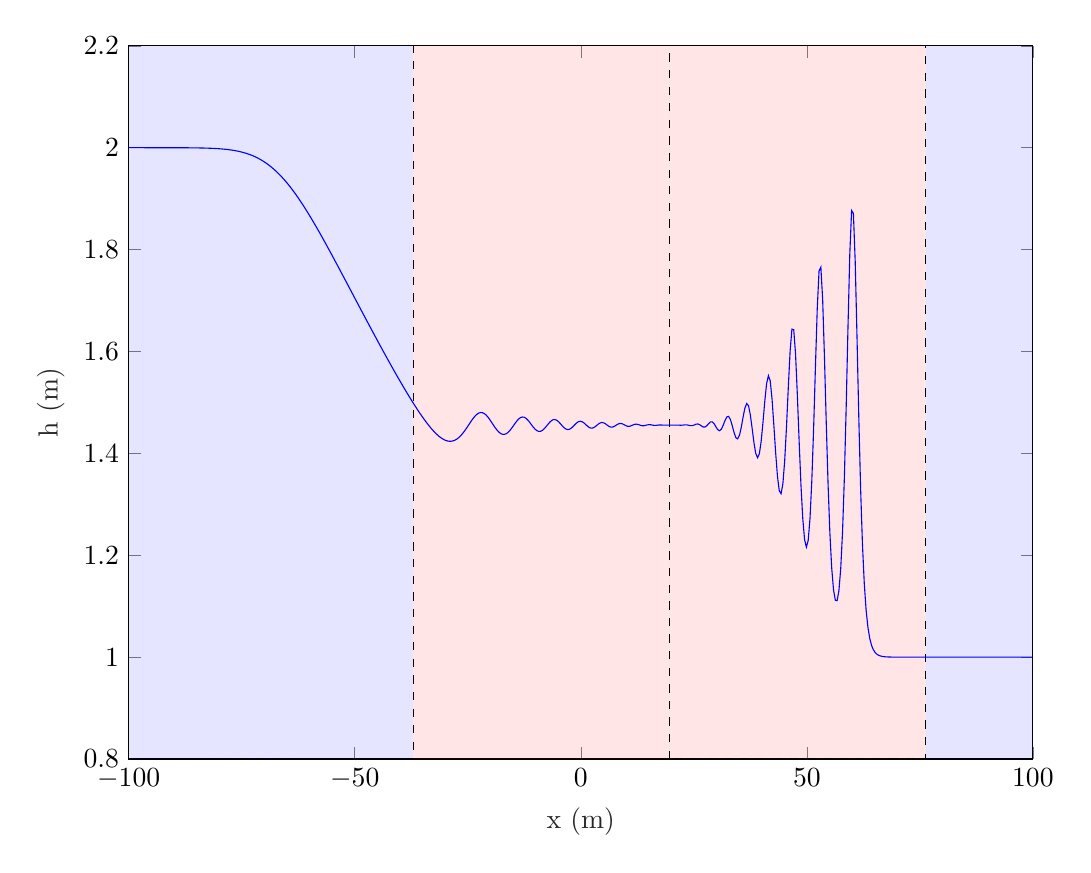
\begin{tikzpicture}

\begin{axis}[%
width=4.521in,
height=3.566in,
at={(0.758in,0.481in)},
scale only axis,
xmin=-100,
xmax=100,
xtick={-100,  -50,    0,   50,  100},
xlabel style={font=\color{white!15!black}},
xlabel={x (m)},
ymin=0.8,
ymax=2.2,
ytick={0.8,   1, 1.2, 1.4, 1.6, 1.8,   2, 2.2},
ylabel style={font=\color{white!15!black}},
ylabel={h (m)},
axis background/.style={fill=white}
]

\addplot[area legend, dashed, draw=black, fill=blue, fill opacity=0.1, forget plot]
table[row sep=crcr] {%
x	y\\
-100	0.8\\
-100	2.2\\
-37.0630892039997	2.2\\
-37.0630892039997	0.8\\
}--cycle;

\addplot[area legend, draw=none, fill=red, fill opacity=0.1, forget plot]
table[row sep=crcr] {%
x	y\\
-37.0630892039997	0.8\\
-37.0630892039997	2.2\\
19.5890566189392	2.2\\
19.5890566189392	0.8\\
}--cycle;

\addplot[area legend, draw=none, fill=green, fill opacity=0.1, forget plot]
table[row sep=crcr] {%
x	y\\
19.5890566189392	0.8\\
19.5890566189392	2.2\\
19.5890566189392	2.2\\
19.5890566189392	0.8\\
}--cycle;

\addplot[area legend, draw=none, fill=green, fill opacity=0.1, forget plot]
table[row sep=crcr] {%
x	y\\
19.5890566189392	0.8\\
19.5890566189392	2.2\\
19.5890566189392	2.2\\
19.5890566189392	0.8\\
}--cycle;

\addplot[area legend, dashed, draw=black, fill=red, fill opacity=0.1, forget plot]
table[row sep=crcr] {%
x	y\\
19.5890566189392	0.8\\
19.5890566189392	2.2\\
76.2412024418781	2.2\\
76.2412024418781	0.8\\
}--cycle;

\addplot[area legend, draw=none, fill=blue, fill opacity=0.1, forget plot]
table[row sep=crcr] {%
x	y\\
76.2412024418781	0.8\\
76.2412024418781	2.2\\
100	2.2\\
100	0.8\\
}--cycle;
\addplot [color=blue, forget plot]
  table[row sep=crcr]{%
-100.1200120012	2\\
-99.7199719971997	1.99999781748578\\
-99.3199319931993	1.9999977280879\\
-98.9198919891989	1.99999757291011\\
-98.5198519851985	1.99999734825528\\
-98.1198119811981	1.99999704831281\\
-97.7197719771977	1.99999666536311\\
-97.3197319731973	1.99999618961255\\
-96.9196919691969	1.9999956089797\\
-96.5196519651965	1.99999490883398\\
-96.1196119611961	1.99999407168266\\
-95.7195719571957	1.99999307680091\\
-95.3195319531953	1.99999189979901\\
-94.9194919491949	1.99999051211997\\
-94.5194519451945	1.99998888045983\\
-94.1194119411941	1.99998696610202\\
-93.7193719371937	1.99998472415599\\
-93.3193319331933	1.99998210268965\\
-92.9192919291929	1.99997904174339\\
-92.5192519251925	1.99997547221312\\
-92.1192119211921	1.99997131458779\\
-91.7191719171917	1.99996647752629\\
-91.3191319131913	1.99996085625685\\
-90.9190919091909	1.99995433078149\\
-90.5190519051905	1.9999467638661\\
-90.1190119011901	1.9999379987964\\
-89.7189718971897	1.9999278568785\\
-89.3189318931893	1.99991613466196\\
-88.9188918891889	1.99990260086288\\
-88.5188518851885	1.99988699296352\\
-88.1188118811881	1.9998690134654\\
-87.7187718771877	1.9998483257725\\
-87.3187318731873	1.9998245496823\\
-86.9186918691869	1.99979725646321\\
-86.5186518651865	1.99976596349912\\
-86.1186118611861	1.99973012848413\\
-85.7185718571857	1.99968914315415\\
-85.3185318531853	1.99964232654634\\
-84.9184918491849	1.99958891778285\\
-84.5184518451845	1.99952806838211\\
-84.1184118411841	1.99945883410871\\
-83.7183718371837	1.9993801663825\\
-83.3183318331833	1.9992909032782\\
-82.9182918291829	1.99918976015926\\
-82.5182518251825	1.99907532000387\\
-82.1182118211821	1.99894602349614\\
-81.7181718171817	1.99880015897294\\
-81.3181318131813	1.99863585233487\\
-80.9180918091809	1.99845105704981\\
-80.5180518051805	1.99824354439761\\
-80.1180118011801	1.99801089412594\\
-79.7179717971797	1.99775048570828\\
-79.3179317931793	1.99745949041593\\
-78.9178917891789	1.99713486443553\\
-78.5178517851785	1.99677334328155\\
-78.1178117811781	1.99637143776831\\
-77.7177717771777	1.99592543181763\\
-77.3177317731773	1.99543138238514\\
-76.9176917691769	1.99488512178952\\
-76.5176517651765	1.99428226272348\\
-76.1176117611761	1.99361820621211\\
-75.7175717571757	1.99288815276253\\
-75.3175317531753	1.9920871169175\\
-74.9174917491749	1.99120994538482\\
-74.5174517451745	1.99025133886304\\
-74.1174117411741	1.98920587762275\\
-73.7173717371737	1.98806805083189\\
-73.3173317331733	1.98683228953401\\
-72.9172917291729	1.9854930031015\\
-72.5172517251725	1.98404461889368\\
-72.1172117211721	1.98248162475439\\
-71.7171717171717	1.98079861388827\\
-71.3171317131713	1.97899033156256\\
-70.9170917091709	1.97705172299507\\
-70.5170517051705	1.97497798171311\\
-70.1170117011701	1.97276459760538\\
-69.7169716971697	1.97040740384364\\
-69.3169316931693	1.96790262182469\\
-68.9168916891689	1.96524690328018\\
-68.5168516851685	1.96243736872196\\
-68.1168116811681	1.95947164143563\\
-67.7167716771677	1.95634787630512\\
-67.3167316731673	1.95306478284331\\
-66.9166916691669	1.94962164191806\\
-66.5166516651665	1.94601831579417\\
-66.1166116611661	1.94225525125722\\
-65.7165716571657	1.9383334757387\\
-65.3165316531653	1.93425458651958\\
-64.9164916491649	1.93002073324461\\
-64.5164516451645	1.92563459412783\\
-64.1164116411641	1.92109934636522\\
-63.7163716371637	1.91641863138919\\
-63.3163316331633	1.91159651569739\\
-62.9162916291629	1.90663744806288\\
-62.5162516251625	1.90154621398204\\
-62.1162116211621	1.89632788823995\\
-61.7161716171617	1.89098778647142\\
-61.3161316131613	1.88553141656968\\
-60.9160916091609	1.87996443074782\\
-60.5160516051605	1.87429257899188\\
-60.1160116011601	1.86852166456364\\
-59.7159715971597	1.86265750211888\\
-59.3159315931593	1.85670587890748\\
-58.9158915891589	1.85067251941866\\
-58.5158515851585	1.84456305373198\\
-58.1158115811581	1.83838298973522\\
-57.7157715771577	1.83213768927698\\
-57.3157315731573	1.82583234823685\\
-56.9156915691569	1.81947198042119\\
-56.5156515651565	1.81306140512828\\
-56.1156115611561	1.80660523817472\\
-55.7155715571557	1.8001078861339\\
-55.3155315531553	1.79357354350845\\
-54.9154915491549	1.78700619253957\\
-54.5154515451545	1.78040960534755\\
-54.1154115411541	1.77378734809704\\
-53.7153715371537	1.76714278688824\\
-53.3153315331533	1.76047909508751\\
-52.9152915291529	1.75379926182958\\
-52.5152515251525	1.74710610144461\\
-52.1152115211521	1.74040226358763\\
-51.7151715171517	1.73369024387347\\
-51.3151315131513	1.72697239484647\\
-50.9150915091509	1.72025093714074\\
-50.5150515051505	1.71352797071215\\
-50.1150115011501	1.70680548604771\\
-49.7149714971497	1.70008537528177\\
-49.3149314931493	1.69336944316926\\
-48.9148914891489	1.68665941788714\\
-48.5148514851485	1.67995696165279\\
-48.1148114811481	1.67326368116549\\
-47.7147714771477	1.66658113789211\\
-47.3147314731473	1.65991085823238\\
-46.9146914691469	1.6532543436123\\
-46.5146514651465	1.64661308056631\\
-46.1146114611461	1.63998855088104\\
-45.7145714571457	1.63338224188478\\
-45.3145314531453	1.62679565697891\\
-44.9144914491449	1.62023032651982\\
-44.5144514451445	1.61368781917285\\
-44.1144114411441	1.60716975387444\\
-43.7143714371437	1.6006778125546\\
-43.3143314331433	1.59421375378986\\
-42.9142914291429	1.58777942757742\\
-42.5142514251425	1.5813767914449\\
-42.1142114211421	1.57500792813661\\
-41.7141714171417	1.5686750651485\\
-41.3141314131413	1.56238059641892\\
-40.9140914091409	1.55612710652278\\
-40.5140514051405	1.54991739776207\\
-40.1140114011401	1.54375452059743\\
-39.7139713971397	1.53764180792286\\
-39.3139313931393	1.53158291374962\\
-38.9138913891389	1.52558185693471\\
-38.5138513851385	1.51964307066421\\
-38.1138113811381	1.51377145847995\\
-37.7137713771377	1.50797245771646\\
-37.3137313731373	1.50225211129049\\
-36.9136913691369	1.49661714884998\\
-36.5136513651365	1.49107507833374\\
-36.1136113611361	1.48563428900288\\
-35.7135713571357	1.48030416696039\\
-35.3135313531353	1.47509522404749\\
-34.9134913491349	1.47001924075649\\
-34.5134513451345	1.46508942337737\\
-34.1134113411341	1.46032057492994\\
-33.7133713371337	1.45572927843308\\
-33.3133313331333	1.45133408961062\\
-32.9132913291329	1.44715573408065\\
-32.5132513251325	1.44321730123878\\
-32.1132113211321	1.43954442321136\\
-31.7131713171317	1.43616542217773\\
-31.3131313131313	1.43311140278963\\
-30.9130913091309	1.4304162581254\\
-30.5130513051305	1.42811654747285\\
-30.1130113011301	1.42625119229791\\
-29.7129712971297	1.42486092344666\\
-29.3129312931293	1.4239873989473\\
-28.9128912891289	1.42367165021514\\
-28.5128512851285	1.42395350406744\\
-28.1128112811281	1.42486663579472\\
-27.7127712771277	1.42643791666258\\
-27.3127312731273	1.42868228329337\\
-26.9126912691269	1.43159839127819\\
-26.5126512651265	1.43516347967798\\
-26.1126112611261	1.43932801955251\\
-25.7125712571257	1.44401064858559\\
-25.3125312531253	1.44909417627835\\
-24.9124912491249	1.4544235928695\\
-24.5124512451245	1.45980715687706\\
-24.1124112411241	1.4650215825379\\
-23.7123712371237	1.46982202931116\\
-23.3123312331233	1.4739570223836\\
-22.9122912291229	1.47718755639237\\
-22.5122512251225	1.47930868691802\\
-22.1122112211221	1.48017107423069\\
-21.7121712171217	1.4796991115931\\
-21.3121312131213	1.47790366155762\\
-20.9120912091209	1.47488563849869\\
-20.5120512051205	1.47083129147642\\
-20.1120112011201	1.46599888188539\\
-19.7119711971197	1.46069912824324\\
-19.3119311931193	1.45527212285848\\
-18.9118911891189	1.45006354819822\\
-18.5118511851185	1.44540245067265\\
-18.1118111811181	1.44158191026389\\
-17.7117711771177	1.43884297514317\\
-17.3117311731173	1.43736150011235\\
-16.9116911691169	1.43723722912118\\
-16.5116511651165	1.43848459766632\\
-16.1116111611161	1.44102549529931\\
-15.7115711571157	1.44468502419666\\
-15.3115311531153	1.44919241504538\\
-14.9114911491149	1.45418994697839\\
-14.5114511451145	1.45925270245575\\
-14.1114111411141	1.46392086738704\\
-13.7113711371137	1.46774386711389\\
-13.3113311331133	1.47033229379527\\
-12.9112911291129	1.4714101582753\\
-12.5112511251125	1.47085796680109\\
-12.1112111211121	1.46873722431902\\
-11.7111711171117	1.46529031280178\\
-11.3111311131113	1.46091459825156\\
-10.9110911091109	1.45611511124579\\
-10.5110511051105	1.45144393867465\\
-10.1110111011101	1.4474356419001\\
-9.71097109710971	1.44454677638463\\
-9.3109310931093	1.44310498974663\\
-8.9108910891089	1.44327084039751\\
-8.51085108510851	1.44501429435475\\
-8.11081108110811	1.44810849576695\\
-7.71077107710771	1.45214418695451\\
-7.31073107310731	1.45656877618385\\
-6.9106910691069	1.46075191759482\\
-6.5106510651065	1.46407421917074\\
-6.11061106110611	1.46602784218673\\
-5.71057105710571	1.46631017497375\\
-5.31053105310531	1.46488844843615\\
-4.91049104910491	1.46201688343969\\
-4.5104510451045	1.45819887554281\\
-4.1104110411041	1.45410076409572\\
-3.71037103710371	1.45043496072541\\
-3.31033103310331	1.44783533546142\\
-2.91029102910291	1.44674616337577\\
-2.51025102510251	1.44734181797733\\
-2.1102110211021	1.44948677375862\\
-1.7101710171017	1.45274830622943\\
-1.31013101310131	1.45646327410948\\
-0.91009100910091	1.4598592509334\\
-0.510051005100507	1.46221415625063\\
-0.110011001100105	1.46302212687137\\
0.290029002900297	1.46212695734443\\
0.6900690069007	1.45976705310875\\
1.09010901090109	1.4565337290259\\
1.49014901490149	1.45322715821366\\
1.89018901890189	1.4506602712077\\
2.2902290229023	1.44945604113091\\
2.6902690269027	1.44988773439949\\
3.0903090309031	1.45180069249898\\
3.4903490349035	1.4546390825873\\
3.89038903890389	1.45758294592688\\
4.29042904290429	1.45977371980399\\
4.6904690469047	1.46057287063504\\
5.0905090509051	1.45977389421411\\
5.4905490549055	1.45768038622213\\
5.8905890589059	1.45501841721018\\
6.29062906290629	1.45269510042061\\
6.69066906690669	1.45148928230975\\
7.0907090709071	1.45177828600784\\
7.4907490749075	1.45339627057796\\
7.8907890789079	1.45568324655261\\
8.2908290829083	1.45772507064404\\
8.69086908690869	1.45871355105271\\
9.09090909090909	1.4582889483394\\
9.4909490949095	1.45670551298392\\
9.8909890989099	1.45472582399868\\
10.2910291029103	1.45327245425477\\
10.6910691069107	1.45299285459028\\
11.0911091109111	1.45394380020301\\
11.4911491149115	1.45555959993582\\
11.8911891189119	1.45694414673792\\
12.2912291229123	1.45736018257872\\
12.6912691269127	1.45665391117377\\
13.0913091309131	1.45534267008718\\
13.4913491349135	1.45428693016558\\
13.8913891389139	1.45412854379343\\
14.2914291429143	1.4548663935545\\
14.6914691469147	1.45587529935316\\
15.0915091509151	1.4563869847315\\
15.4915491549155	1.45608616992295\\
15.8915891589159	1.45534812503707\\
16.2916291629163	1.45486543188049\\
16.6916691669167	1.45500373057814\\
17.0917091709171	1.45549045626628\\
17.4917491749175	1.45576660121919\\
17.8917891789179	1.45561455777207\\
18.2918291829183	1.45534034143404\\
18.6918691869187	1.45528997436197\\
19.0919091909191	1.4554158295877\\
19.4919491949195	1.45547946895232\\
19.8919891989199	1.45543775240816\\
20.2920292029203	1.45541357094366\\
20.6920692069207	1.45544047912788\\
21.0921092109211	1.45547351638544\\
21.4921492149215	1.45541144986124\\
21.8921892189219	1.4552637572834\\
22.2922292229223	1.45525398977851\\
22.6922692269227	1.45556041895947\\
23.0923092309231	1.45592503239195\\
23.4923492349235	1.45580703776988\\
23.8923892389239	1.45506051992393\\
24.2924292429243	1.45430708884514\\
24.6924692469247	1.45443882902956\\
25.0925092509251	1.45569037694827\\
25.4925492549255	1.45721986523996\\
25.8925892589259	1.45767207343366\\
26.2926292629263	1.45630184102913\\
26.6926692669267	1.45372220739626\\
27.0927092709271	1.45163637701574\\
27.4927492749275	1.45172011467161\\
27.8927892789279	1.45443757779123\\
28.2928292829283	1.45856449460107\\
28.6928692869287	1.46174139105374\\
29.0929092909291	1.46179126441073\\
29.4929492949295	1.4580626010675\\
29.8929892989299	1.45197643045593\\
30.2930293029303	1.44642660373611\\
30.6930693069307	1.44438826272686\\
31.0931093109311	1.44749994878839\\
31.4931493149315	1.45513777318404\\
31.8931893189319	1.46448353785773\\
32.2932293229323	1.47148604925076\\
32.6932693269327	1.47256386838222\\
33.0933093309331	1.46632021556601\\
33.4933493349335	1.45437785367663\\
33.8933893389339	1.44084843900458\\
34.2934293429343	1.43077366166565\\
34.6934693469347	1.42833904199916\\
35.0935093509351	1.43548273438504\\
35.4935493549355	1.45112701299863\\
35.8935893589359	1.47109170197213\\
36.2936293629363	1.48893457366657\\
36.6936693669367	1.49789368721459\\
37.0937093709371	1.49352055034916\\
37.4937493749375	1.47575407618915\\
37.8937893789379	1.44916526420807\\
38.2938293829383	1.42124331566037\\
38.6938693869387	1.39988834608437\\
39.0939093909391	1.39139622089605\\
39.4939493949395	1.39928420508518\\
39.8939893989399	1.4237150317991\\
40.2940294029403	1.46082209453588\\
40.6940694069407	1.50241674590247\\
41.0941094109411	1.53692770012374\\
41.4941494149415	1.55259646457913\\
41.8941894189419	1.5423093483667\\
42.2942294229423	1.50712262273503\\
42.6942694269427	1.45591141068378\\
43.0943094309431	1.4013291027216\\
43.4943494349435	1.3553069024865\\
43.8943894389439	1.32662299693583\\
44.2944294429443	1.32070544663242\\
44.6944694469447	1.34026769292917\\
45.0945094509451	1.38532528115925\\
45.4945494549455	1.45184480962855\\
45.8945894589459	1.52949263129313\\
46.2946294629463	1.600628926898\\
46.6946694669467	1.64381298314905\\
47.0947094709471	1.64273425701851\\
47.4947494749475	1.59532731966448\\
47.8947894789479	1.51503924358175\\
48.2948294829483	1.42294015424434\\
48.6948694869487	1.33794847907368\\
49.0949094909491	1.27198425905305\\
49.4949494949495	1.23058230196905\\
49.8949894989499	1.21586542337367\\
50.2950295029503	1.22914749696961\\
50.6950695069507	1.27218497040102\\
51.0951095109511	1.34625363688035\\
51.4951495149515	1.44901847516262\\
51.8951895189519	1.56938571489669\\
52.2952295229523	1.68346546591578\\
52.6952695269527	1.7580595773841\\
53.0953095309531	1.76557902900409\\
53.4953495349535	1.70159974828626\\
53.8953895389539	1.58795509050837\\
54.2954295429543	1.45782731084826\\
54.6954695469547	1.33823655218954\\
55.0955095509551	1.24296017567447\\
55.4955495549555	1.17505746237805\\
55.8955895589559	1.13232483443083\\
56.2956295629563	1.11156357359603\\
56.6956695669567	1.11091962413231\\
57.0957095709571	1.13089184673303\\
57.4957495749575	1.17453484312747\\
57.8957895789579	1.24680873887122\\
58.2958295829583	1.35233382451031\\
58.6958695869587	1.49041879144974\\
59.0959095909591	1.6474143700013\\
59.4959495949595	1.79100323039497\\
59.8959895989599	1.87661118107627\\
60.2960296029603	1.87090354783523\\
60.6960696069607	1.77571686064355\\
61.0961096109611	1.62657158618303\\
61.4961496149615	1.46746456566645\\
61.8961896189619	1.3285958655812\\
62.2962296229623	1.22147230322021\\
62.6962696269627	1.14509098235283\\
63.0963096309631	1.09329835036311\\
63.4963496349635	1.05928099348447\\
63.8963896389639	1.03738297513812\\
64.2964296429643	1.02346290370282\\
64.6964696469647	1.01468334472465\\
65.0965096509651	1.0091727773409\\
65.4965496549655	1.00572430625456\\
65.8965896589659	1.00357016744713\\
66.2966296629663	1.0022259880287\\
66.6966696669667	1.0013877297854\\
67.0967096709671	1.00086513896581\\
67.4967496749675	1.0005393854167\\
67.8967896789679	1.00033633151747\\
68.2968296829683	1.00020975245428\\
68.6968696869687	1.00013083675871\\
69.0969096909691	1.0000816292055\\
69.4969496949695	1.00005094047697\\
69.8969896989699	1.00003179728817\\
70.2970297029703	1.00001985338828\\
70.6970697069707	1.00001239951316\\
71.0971097109711	1.00000774655055\\
71.4971497149715	1.00000484121694\\
71.8971897189719	1.00000302658216\\
72.2972297229723	1.00000189283181\\
72.6972697269727	1.00000118425111\\
73.0973097309731	1.00000074124042\\
73.4973497349735	1.00000046416242\\
73.8973897389739	1.00000029079661\\
74.2974297429743	1.00000018227659\\
74.6974697469747	1.00000011431657\\
75.0975097509751	1.00000007173642\\
75.4975497549755	1.00000004504418\\
75.8975897589759	1.00000002830241\\
76.2976297629763	1.00000001779557\\
76.6976697669767	1.00000001119755\\
77.0977097709771	1.00000000705142\\
77.4977497749775	1.0000000044442\\
77.8977897789779	1.00000000280345\\
78.2978297829783	1.00000000177011\\
78.6978697869787	1.00000000111875\\
79.0979097909791	1.00000000070781\\
79.4979497949795	1.0000000004483\\
79.8979897989799	1.00000000028426\\
80.2980298029803	1.00000000018046\\
80.6980698069807	1.0000000001147\\
81.0981098109811	1.000000000073\\
81.4981498149815	1.00000000004652\\
81.8981898189819	1.00000000002969\\
82.2982298229823	1.00000000001897\\
82.6982698269827	1.00000000001213\\
83.0983098309831	1.00000000000777\\
83.4983498349835	1.00000000000498\\
83.8983898389839	1.0000000000032\\
84.2984298429843	1.00000000000205\\
84.6984698469847	1.00000000000132\\
85.0985098509851	1.00000000000085\\
85.4985498549855	1.00000000000054\\
85.8985898589859	1.00000000000035\\
86.2986298629863	1.00000000000022\\
86.6986698669867	1.00000000000014\\
87.0987098709871	1.00000000000008\\
87.4987498749875	1.00000000000005\\
87.8987898789879	1.00000000000003\\
88.2988298829883	1.00000000000001\\
88.6988698869887	1\\
89.0989098909891	1\\
89.4989498949895	1\\
89.8989898989899	1\\
90.2990299029903	1\\
90.6990699069907	1\\
91.0991099109911	1\\
91.4991499149915	1\\
91.8991899189919	1\\
92.2992299229923	1\\
92.6992699269927	1\\
93.0993099309931	1\\
93.4993499349935	1\\
93.8993899389939	1\\
94.2994299429943	1\\
94.6994699469947	1\\
95.0995099509951	1\\
95.4995499549955	1\\
95.8995899589959	1\\
96.2996299629963	1\\
96.6996699669967	1\\
97.0997099709971	1\\
97.4997499749975	1\\
97.8997899789979	1\\
98.2998299829983	1\\
98.6998699869987	1\\
99.0999099909991	1\\
99.4999499949995	1\\
99.8999899989999	1\\
};
\end{axis}
\end{tikzpicture}%
		\caption{$h$}
	\end{subfigure}
	\begin{subfigure}{0.49\textwidth}
		\centering
		% This file was created by matlab2tikz.
%
%The latest updates can be retrieved from
%  http://www.mathworks.com/matlabcentral/fileexchange/22022-matlab2tikz-matlab2tikz
%where you can also make suggestions and rate matlab2tikz.
%
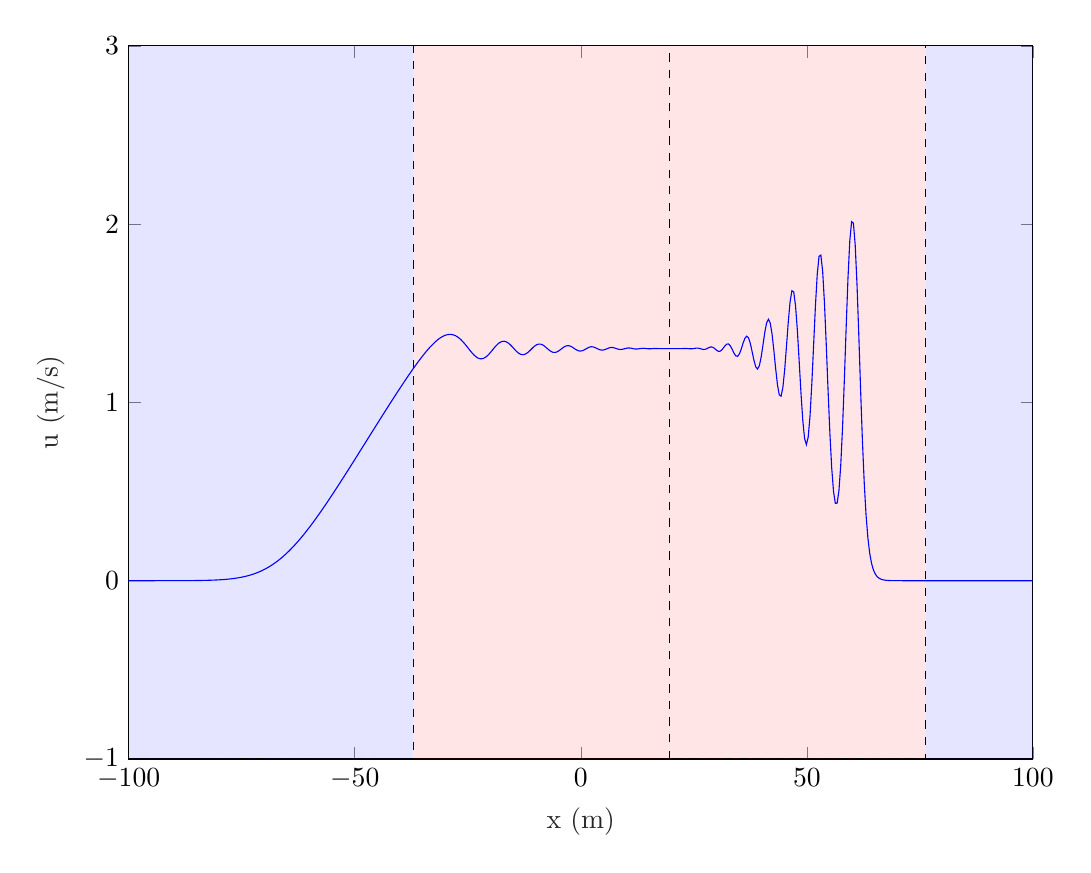
\begin{tikzpicture}

\begin{axis}[%
width=4.521in,
height=3.566in,
at={(0.758in,0.481in)},
scale only axis,
xmin=-100,
xmax=100,
xtick={-100,  -50,    0,   50,  100},
xlabel style={font=\color{white!15!black}},
xlabel={x (m)},
ymin=-1,
ymax=3,
ytick={-1,  0,  1,  2,  3},
ylabel style={font=\color{white!15!black}},
ylabel={u (m/s)},
axis background/.style={fill=white}
]

\addplot[area legend, dashed, draw=black, fill=blue, fill opacity=0.1, forget plot]
table[row sep=crcr] {%
x	y\\
-100	-1\\
-100	3\\
-37.0630892039997	3\\
-37.0630892039997	-1\\
}--cycle;

\addplot[area legend, draw=none, fill=red, fill opacity=0.1, forget plot]
table[row sep=crcr] {%
x	y\\
-37.0630892039997	-1\\
-37.0630892039997	3\\
19.5890566189392	3\\
19.5890566189392	-1\\
}--cycle;

\addplot[area legend, draw=none, fill=green, fill opacity=0.1, forget plot]
table[row sep=crcr] {%
x	y\\
19.5890566189392	-1\\
19.5890566189392	3\\
19.5890566189392	3\\
19.5890566189392	-1\\
}--cycle;

\addplot[area legend, draw=none, fill=green, fill opacity=0.1, forget plot]
table[row sep=crcr] {%
x	y\\
19.5890566189392	-1\\
19.5890566189392	3\\
19.5890566189392	3\\
19.5890566189392	-1\\
}--cycle;

\addplot[area legend, dashed, draw=black, fill=red, fill opacity=0.1, forget plot]
table[row sep=crcr] {%
x	y\\
19.5890566189392	-1\\
19.5890566189392	3\\
76.2412024418781	3\\
76.2412024418781	-1\\
}--cycle;

\addplot[area legend, draw=none, fill=blue, fill opacity=0.1, forget plot]
table[row sep=crcr] {%
x	y\\
76.2412024418781	-1\\
76.2412024418781	3\\
100	3\\
100	-1\\
}--cycle;
\addplot [color=blue, forget plot]
  table[row sep=crcr]{%
-100.1200120012	0\\
-99.7199719971997	8.61891600267421e-07\\
-99.3199319931993	1.81998374191612e-06\\
-98.9198919891989	2.82752926907882e-06\\
-98.5198519851985	3.91157130997584e-06\\
-98.1198119811981	5.10089757569374e-06\\
-97.7197719771977	6.42677595377539e-06\\
-97.3197319731973	7.9236679715355e-06\\
-96.9196919691969	9.63000355635629e-06\\
-96.5196519651965	1.15890307461857e-05\\
-96.1196119611961	1.3849755230288e-05\\
-95.7195719571957	1.64679857289699e-05\\
-95.3195319531953	1.95075024643177e-05\\
-94.9194919491949	2.30413674369565e-05\\
-94.5194519451945	2.71533967877833e-05\\
-94.1194119411941	3.1939817270181e-05\\
-93.7193719371937	3.75111307339591e-05\\
-93.3193319331933	4.39942125389152e-05\\
-92.9192919291929	5.15346719648975e-05\\
-92.5192519251925	6.02995048778248e-05\\
-92.1192119211921	7.04800712701119e-05\\
-91.7191719171917	8.22954326122142e-05\\
-91.3191319131913	9.59960863192152e-05\\
-90.9190919091909	0.000111868136956756\\
-90.5190519051905	0.000130237946005697\\
-90.1190119011901	0.000151477304064984\\
-89.7189718971897	0.000176009171150133\\
-89.3189318931893	0.000204314032184559\\
-88.9188918891889	0.000236936915783294\\
-88.5188518851885	0.000274495124804275\\
-88.1188118811881	0.000317686726863853\\
-87.7187718771877	0.00036729985179747\\
-87.3187318731873	0.000424222840810112\\
-86.9186918691869	0.000489455288599339\\
-86.5186518651865	0.000564120014823161\\
-86.1186118611861	0.000649475994727216\\
-85.7185718571857	0.000746932270355253\\
-85.3185318531853	0.000858062853269755\\
-84.9184918491849	0.000984622616928339\\
-84.5184518451845	0.00112856416156229\\
-84.1184118411841	0.00129205561648694\\
-83.7183718371837	0.00147749932388354\\
-83.3183318331833	0.00168755132441427\\
-82.9182918291829	0.00192514153820646\\
-82.5182518251825	0.00219349450503089\\
-82.1182118211821	0.00249615051482669\\
-81.7181718171817	0.00283698692450329\\
-81.3181318131813	0.00322023941922331\\
-80.9180918091809	0.00365052293701189\\
-80.5180518051805	0.00413285193480793\\
-80.1180118011801	0.00467265963301839\\
-79.7179717971797	0.00527581583514106\\
-79.3179317931793	0.00594864288031617\\
-78.9178917891789	0.00669792925103286\\
-78.5178517851785	0.00753094032718643\\
-78.1178117811781	0.00845542575299994\\
-77.7177717771777	0.00947962286661101\\
-77.3177317731773	0.0106122556353452\\
-76.9176917691769	0.0118625285446502\\
-76.5176517651765	0.0132401149071304\\
-76.1176117611761	0.0147551390917207\\
-75.7175717571757	0.0164181522232304\\
-75.3175317531753	0.018240100970238\\
-74.9174917491749	0.0202322891253128\\
-74.5174517451745	0.0224063317858416\\
-74.1174117411741	0.0247741020656769\\
-73.7173717371737	0.0273476704063611\\
-73.3173317331733	0.0301392367093796\\
-72.9172917291729	0.0331610556753472\\
-72.5172517251725	0.0364253559081906\\
-72.1172117211721	0.0399442535180994\\
-71.7171717171717	0.0437296611311744\\
-71.3171317131713	0.0477931933806703\\
-70.9170917091709	0.0521460701087356\\
-70.5170517051705	0.0567990186424434\\
-70.1170117011701	0.0617621766179231\\
-69.7169716971697	0.0670449969060538\\
-69.3169316931693	0.0726561562376085\\
-68.9168916891689	0.0786034691312906\\
-68.5168516851685	0.0848938086919987\\
-68.1168116811681	0.0915330357679018\\
-67.7167716771677	0.098525937833642\\
-67.3167316731673	0.105876178805444\\
-66.9166916691669	0.113586260795524\\
-66.5166516651665	0.121657498583268\\
-66.1166116611661	0.130090007325642\\
-65.7165716571657	0.138882703756922\\
-65.3165316531653	0.148033320846519\\
-64.9164916491649	0.157538435602376\\
-64.5164516451645	0.167393509435039\\
-64.1164116411641	0.177592940242741\\
-63.7163716371637	0.188130125148609\\
-63.3163316331633	0.198997532624095\\
-62.9162916291629	0.210186782573637\\
-62.5162516251625	0.221688732838136\\
-62.1162116211621	0.233493570501466\\
-61.7161716171617	0.245590906355257\\
-61.3161316131613	0.257969870891658\\
-60.9160916091609	0.270619210248822\\
-60.5160516051605	0.283527380625595\\
-60.1160116011601	0.296682639804936\\
-59.7159715971597	0.31007313457446\\
-59.3159315931593	0.323686983000201\\
-58.9158915891589	0.337512350690274\\
-58.5158515851585	0.351537520371531\\
-58.1158115811581	0.365750954288928\\
-57.7157715771577	0.380141349118152\\
-57.3157315731573	0.39469768325279\\
-56.9156915691569	0.409409256483612\\
-56.5156515651565	0.424265722226771\\
-56.1156115611561	0.439257112577446\\
-55.7155715571557	0.454373856564761\\
-55.3155315531553	0.469606792062283\\
-54.9154915491549	0.484947171866294\\
-54.5154515451545	0.500386664492569\\
-54.1154115411541	0.515917350262741\\
-53.7153715371537	0.531531713255587\\
-53.3153315331533	0.547222629688745\\
-52.9152915291529	0.562983353274579\\
-52.5152515251525	0.578807498062219\\
-52.1152115211521	0.594689019238949\\
-51.7151715171517	0.610622192319342\\
-51.3151315131513	0.626601591102167\\
-50.9150915091509	0.642622064724732\\
-50.5150515051505	0.658678714092893\\
-50.1150115011501	0.674766867914281\\
-49.7149714971497	0.690882058512504\\
-49.3149314931493	0.707019997552399\\
-48.9148914891489	0.723176551760779\\
-48.5148514851485	0.739347718683948\\
-48.1148114811481	0.755529602482799\\
-47.7147714771477	0.771718389727752\\
-47.3147314731473	0.787910325119603\\
-46.9146914691469	0.804101687027476\\
-46.5146514651465	0.820288762701616\\
-46.1146114611461	0.836467822985388\\
-45.7145714571457	0.852635096317636\\
-45.3145314531453	0.868786741782165\\
-44.9144914491449	0.884918820925067\\
-44.5144514451445	0.901027268021745\\
-44.1144114411441	0.91710785843328\\
-43.7143714371437	0.933156174644721\\
-43.3143314331433	0.949167569525101\\
-42.9142914291429	0.965137126289628\\
-42.5142514251425	0.981059614576766\\
-42.1142114211421	0.996929441976063\\
-41.7141714171417	1.0127406002552\\
-41.3141314131413	1.02848660543531\\
-40.9140914091409	1.04416043075136\\
-40.5140514051405	1.059754431408\\
-40.1140114011401	1.07526025990033\\
-39.7139713971397	1.0906687705129\\
-39.3139313931393	1.1059699114409\\
-38.9138913891389	1.12115260279471\\
-38.5138513851385	1.13620459855982\\
-38.1138113811381	1.15111233039251\\
-37.7137713771377	1.16586073095025\\
-37.3137313731373	1.18043303430011\\
-36.9136913691369	1.19481055084272\\
-36.5136513651365	1.2089724141685\\
-36.1136113611361	1.22289529737479\\
-35.7135713571357	1.23655309668589\\
-35.3135313531353	1.24991658082375\\
-34.9134913491349	1.2629530056002\\
-34.5134513451345	1.27562569480504\\
-34.1134113411341	1.28789359086159\\
-33.7133713371337	1.29971078218319\\
-33.3133313331333	1.31102601902801\\
-32.9132913291329	1.32178223632012\\
-32.5132513251325	1.33191611085001\\
-32.1132113211321	1.34135769199309\\
-31.7131713171317	1.35003016008057\\
-31.3131313131313	1.35784978520552\\
-30.9130913091309	1.36472618165569\\
-30.5130513051305	1.3705629789275\\
-30.1130113011301	1.37525905810775\\
-29.7129712971297	1.37871052967935\\
-29.3129312931293	1.38081365096318\\
-28.9128912891289	1.38146889063892\\
-28.5128512851285	1.38058633493272\\
-28.1128112811281	1.37809260377259\\
-27.7127712771277	1.37393927285652\\
-27.3127312731273	1.3681127593208\\
-26.9126912691269	1.36064526910457\\
-26.5126512651265	1.3516261597734\\
-26.1126112611261	1.34121267835504\\
-25.7125712571257	1.32963865974051\\
-25.3125312531253	1.31721945851872\\
-24.9124912491249	1.3043512433151\\
-24.5124512451245	1.29150291433943\\
-24.1124112411241	1.27919940595866\\
-23.7123712371237	1.26799602623708\\
-23.3123312331233	1.25844469866705\\
-22.9122912291229	1.25105434931185\\
-22.5122512251225	1.24624895552718\\
-22.1122112211221	1.24432767337553\\
-21.7121712171217	1.24543177519456\\
-21.3121312131213	1.24952249967257\\
-20.9120912091209	1.25637322811068\\
-20.5120512051205	1.26557704476929\\
-20.1120112011201	1.27656942277312\\
-19.7119711971197	1.28866374437275\\
-19.3119311931193	1.30109615404714\\
-18.9118911891189	1.31307563966224\\
-18.5118511851185	1.32383536323615\\
-18.1118111811181	1.33268196402812\\
-17.7117711771177	1.33904052425835\\
-17.3117311731173	1.34249374236909\\
-16.9116911691169	1.34281424811861\\
-16.5116511651165	1.33998890953013\\
-16.1116111611161	1.33423290774215\\
-15.7115711571157	1.32599076580838\\
-15.3115311531153	1.3159205518101\\
-14.9114911491149	1.30485781629504\\
-14.5114511451145	1.29375743197841\\
-14.1114111411141	1.28361459458149\\
-13.7113711371137	1.27537035311173\\
-13.3113311331133	1.26981126063855\\
-12.9112911291129	1.26747588306245\\
-12.5112511251125	1.26858202589838\\
-12.1112111211121	1.27298672271257\\
-11.7111711171117	1.28018779843706\\
-11.3111311131113	1.28936899923748\\
-10.9110911091109	1.29948526747689\\
-10.5110511051105	1.30937861908103\\
-10.1110111011101	1.31791114053455\\
-9.71097109710971	1.32409970482032\\
-9.3109310931093	1.32723705062958\\
-8.9108910891089	1.32698518791377\\
-8.51085108510851	1.32342932429299\\
-8.11081108110811	1.31708246739255\\
-7.71077107710771	1.30883526007236\\
-7.31073107310731	1.29985062532324\\
-6.9106910691069	1.29141102207812\\
-6.5106510651065	1.28473552136992\\
-6.11061106110611	1.28079260679268\\
-5.71057105710571	1.28013974365985\\
-5.31053105310531	1.28281987183025\\
-4.91049104910491	1.28833825503762\\
-4.5104510451045	1.2957298281203\\
-4.1104110411041	1.3037114938003\\
-3.71037103710371	1.31089755542745\\
-3.31033103310331	1.31604315955767\\
-2.91029102910291	1.31827296555923\\
-2.51025102510251	1.31725169450951\\
-2.1102110211021	1.31326068739527\\
-1.7101710171017	1.30715792777226\\
-1.31013101310131	1.30022092550963\\
-0.91009100910091	1.29389485142735\\
-0.510051005100507	1.28949216919583\\
-0.110011001100105	1.2879060557979\\
0.290029002900297	1.28940327954133\\
0.6900690069007	1.29355025279208\\
1.09010901090109	1.29929988606897\\
1.49014901490149	1.30523005573193\\
1.89018901890189	1.30988626880481\\
2.2902290229023	1.31214868838126\\
2.6902690269027	1.31152839069503\\
3.0903090309031	1.30830740497614\\
3.4903490349035	1.30347156028659\\
3.89038903890389	1.2984421107656\\
4.29042904290429	1.29467135364873\\
4.6904690469047	1.29321467443648\\
5.0905090509051	1.2944075923413\\
5.4905490549055	1.29775460844214\\
5.8905890589059	1.30208019053949\\
6.29062906290629	1.30591096800747\\
6.69066906690669	1.30797637412865\\
7.0907090709071	1.30765781914963\\
7.4907490749075	1.30521598001687\\
7.8907890789079	1.30169289825914\\
8.2908290829083	1.29850839639785\\
8.69086908690869	1.2968961628929\\
9.09090909090909	1.29740285978329\\
9.4909490949095	1.29966339297463\\
9.8909890989099	1.3025669150738\\
10.2910291029103	1.30476371970788\\
10.6910691069107	1.30529912432946\\
11.0911091109111	1.30407077514434\\
11.4911491149115	1.30186254620445\\
11.8911891189119	1.29991382747614\\
12.2912291229123	1.29923888988982\\
12.6912691269127	1.30006934937825\\
13.0913091309131	1.30174971709359\\
13.4913491349135	1.30317024843178\\
13.8913891389139	1.30348778509599\\
14.2914291429143	1.30266614893443\\
14.6914691469147	1.30144832790737\\
15.0915091509151	1.30076469410198\\
15.4915491549155	1.30102044450208\\
15.8915891589159	1.30182997061476\\
16.2916291629163	1.30242335902541\\
16.6916691669167	1.30236131172534\\
17.0917091709171	1.30188435287326\\
17.4917491749175	1.30156269875995\\
17.8917891789179	1.30165649745717\\
18.2918291829183	1.30191734798936\\
18.6918691869187	1.30200921302167\\
19.0919091909191	1.30192262551228\\
19.4919491949195	1.3018532010768\\
19.8919891989199	1.30186855389253\\
20.2920292029203	1.30190982194564\\
20.6920692069207	1.3019390091687\\
21.0921092109211	1.30194240127094\\
21.4921492149215	1.30186826023503\\
21.8921892189219	1.30176137461563\\
22.2922292229223	1.30182712024061\\
22.6922692269227	1.30216454093108\\
23.0923092309231	1.30245806083084\\
23.4923492349235	1.30220146370358\\
23.8923892389239	1.30136075465956\\
24.2924292429243	1.3006726139879\\
24.6924692469247	1.30105968731208\\
25.0925092509251	1.30263585600866\\
25.4925492549255	1.3043147029799\\
25.8925892589259	1.3045291164684\\
26.2926292629263	1.30254062333569\\
26.6926692669267	1.29926994722954\\
27.0927092709271	1.29691998126313\\
27.4927492749275	1.29755446985893\\
27.8927892789279	1.30156588061732\\
28.2928292829283	1.30710634988138\\
28.6928692869287	1.3109445788331\\
29.0929092909291	1.3102778858897\\
29.4929492949295	1.30445558448375\\
29.8929892989299	1.29565233283308\\
30.2930293029303	1.28808152426707\\
30.6930693069307	1.28604842234128\\
31.0931093109311	1.29173159872826\\
31.4931493149315	1.30380234825737\\
31.8931893189319	1.31764960263583\\
32.2932293229323	1.32717340304189\\
32.6932693269327	1.32734650873894\\
33.0933093309331	1.31645023518007\\
33.4933493349335	1.29712008022428\\
33.8933893389339	1.27579081213592\\
34.2934293429343	1.26063958341438\\
34.6934693469347	1.25862164586359\\
35.0935093509351	1.27262930740192\\
35.4935493549355	1.29991284636353\\
35.8935893589359	1.33252277034869\\
36.2936293629363	1.3597127200788\\
36.6936693669367	1.3714247783085\\
37.0937093709371	1.36161203306407\\
37.4937493749375	1.33039689245657\\
37.8937893789379	1.28454655976875\\
38.2938293829383	1.23611586189301\\
38.6938693869387	1.19943874623496\\
39.0939093909391	1.18710527680297\\
39.4939493949395	1.20599766566539\\
39.8939893989399	1.2545810723605\\
40.2940294029403	1.32244982967316\\
40.6940694069407	1.39260412159474\\
41.0941094109411	1.44595295814522\\
41.4941494149415	1.46650835794\\
41.8941894189419	1.44557044113194\\
42.2942294229423	1.38402580941751\\
42.6942694269427	1.29261215318035\\
43.0943094309431	1.19007896418183\\
43.4943494349435	1.09930996471048\\
43.8943894389439	1.0422276825162\\
44.2944294429443	1.03489643729342\\
44.6944694469447	1.08377692015456\\
45.0945094509451	1.1833549407806\\
45.4945494549455	1.31571638249589\\
45.8945894589459	1.45336379696912\\
46.2946294629463	1.56560308789428\\
46.6946694669467	1.62624236158285\\
47.0947094709471	1.61940339682814\\
47.4947494749475	1.54229429712998\\
47.8947894789479	1.40575113077973\\
48.2948294829483	1.23271325062929\\
48.6948694869487	1.05376130816178\\
49.0949094909491	0.900182633995295\\
49.4949494949495	0.79763147193056\\
49.8949894989499	0.763181636179983\\
50.2950295029503	0.805188337362526\\
50.6950695069507	0.922934677888494\\
51.0951095109511	1.10424214131829\\
51.4951495149515	1.32301972382909\\
51.8951895189519	1.54135425696526\\
52.2952295229523	1.71808875224654\\
52.6952695269527	1.8195172717283\\
53.0953095309531	1.82609485090035\\
53.4953495349535	1.7342681841346\\
53.8953895389539	1.55658155027857\\
54.2954295429543	1.32071578781379\\
54.6954695469547	1.06449694576252\\
55.0955095509551	0.825853262150991\\
55.4955495549555	0.632910096079755\\
55.8955895589559	0.500568032369927\\
56.2956295629563	0.434064164288869\\
56.6956695669567	0.435016017479168\\
57.0957095709571	0.50551932641003\\
57.4957495749575	0.648063598937065\\
57.8957895789579	0.860779139491045\\
58.2958295829583	1.12973437403803\\
58.6958695869587	1.42362945632384\\
59.0959095909591	1.6975002451229\\
59.4959495949595	1.90549629461553\\
59.8959895989599	2.01372719752211\\
60.2960296029603	2.00553024424118\\
60.6960696069607	1.88125990185529\\
61.0961096109611	1.65831326031582\\
61.4961496149615	1.37095489389567\\
61.8961896189619	1.06413502112937\\
62.2962296229623	0.779930052601998\\
62.6962696269627	0.544900141305781\\
63.0963096309631	0.36690297974217\\
63.4963496349635	0.240558809877989\\
63.8963896389639	0.154864896128738\\
64.2964296429643	0.0984981933975788\\
64.6964696469647	0.0621600828229964\\
65.0965096509651	0.0390344716887751\\
65.4965496549655	0.0244370888764131\\
65.8965896589659	0.0152698631605216\\
66.2966296629663	0.00953094389416342\\
66.6966696669667	0.00594512633579376\\
67.0967096709671	0.00370717643126248\\
67.4967496749675	0.002311355839682\\
67.8967896789679	0.00144107326390758\\
68.2968296829683	0.000898538352611728\\
68.6968696869687	0.000560328317903767\\
69.0969096909691	0.000349478901461824\\
69.4969496949695	0.000218014112262237\\
69.8969896989699	0.000136032870854615\\
70.2970297029703	8.49000109282694e-05\\
70.6970697069707	5.30010696017445e-05\\
71.0971097109711	3.30965502258242e-05\\
71.4971497149715	2.06733257452743e-05\\
71.8971897189719	1.29174304582467e-05\\
72.2972297229723	8.07400804401957e-06\\
72.6972697269727	5.04846254928644e-06\\
73.0973097309731	3.15788495024752e-06\\
73.4973497349735	1.97611244342957e-06\\
73.8973897389739	1.23713447603695e-06\\
74.2974297429743	7.74862387130618e-07\\
74.6974697469747	4.85565681448691e-07\\
75.0975097509751	3.04439700607401e-07\\
75.4975497549755	1.90985108066045e-07\\
75.8975897589759	1.19883258901464e-07\\
76.2976297629763	7.53000314000221e-08\\
76.6976697669767	4.73289619035721e-08\\
77.0977097709771	2.97695673443348e-08\\
77.4977497749775	1.87392001983623e-08\\
77.8977897789779	1.18054508637471e-08\\
78.2978297829783	7.44368348242934e-09\\
78.6978697869787	4.69773118670865e-09\\
79.0979097909791	2.96759829844446e-09\\
79.4979497949795	1.8765534817583e-09\\
79.8979897989799	1.18789422772494e-09\\
80.2980298029803	7.52794578811239e-10\\
80.6980698069807	4.77616307786608e-10\\
81.0981098109811	3.03392890234456e-10\\
81.4981498149815	1.92962073707268e-10\\
81.8981898189819	1.22882893558651e-10\\
82.2982298229823	7.83579932852214e-11\\
82.6982698269827	5.00313839507697e-11\\
83.0983098309831	3.19856089416129e-11\\
83.4983498349835	2.04737342373031e-11\\
83.8983898389839	1.31186767128465e-11\\
84.2984298429843	8.41379774259568e-12\\
84.6984698469847	5.39967290705538e-12\\
85.0985098509851	3.46547613783308e-12\\
85.4985498549855	2.22245745983309e-12\\
85.8985898589859	1.42179046090557e-12\\
86.2986298629863	9.05597524447312e-13\\
86.6986698669867	5.7212860463274e-13\\
87.0987098709871	3.57044624105539e-13\\
87.4987498749875	2.18477421154496e-13\\
87.8987898789879	1.29990821991196e-13\\
88.2988298829883	7.349478405128e-14\\
88.6988698869887	3.8745727630171e-14\\
89.0989098909891	1.94204664403149e-14\\
89.4989498949895	9.71307111352446e-15\\
89.8989898989899	4.85795491814425e-15\\
90.2990299029903	2.429687347173e-15\\
90.6990699069907	1.21519872137217e-15\\
91.0991099109911	6.07776936461684e-16\\
91.4991499149915	3.03977282067587e-16\\
91.8991899189919	1.52033060930391e-16\\
92.2992299229923	7.60387469044257e-17\\
92.6992699269927	3.80304849180865e-17\\
93.0993099309931	1.90207998152725e-17\\
93.4993499349935	9.51317939701222e-18\\
93.8993899389939	4.75797984769933e-18\\
94.2994299429943	2.37968519827083e-18\\
94.6994699469947	1.19019033131459e-18\\
95.0995099509951	5.95269069302186e-19\\
95.4995499549955	2.97721485376739e-19\\
95.8995899589959	1.48904177754378e-19\\
96.2996299629963	7.44737067826132e-20\\
96.6996699669967	3.72474536155417e-20\\
97.0997099709971	1.86286048177441e-20\\
97.4997499749975	9.315895071947e-21\\
97.8997899789979	4.65705048575682e-21\\
98.2998299829983	2.32469034736372e-21\\
98.6998699869987	1.15365666562524e-21\\
99.0999099909991	5.58945765630972e-22\\
99.4999499949995	2.43462809349053e-22\\
99.8999899989999	4.96045683885341e-23\\
};
\end{axis}
\end{tikzpicture}%
		\caption{$u$}
	\end{subfigure}
	\caption{Solution of gSGN with $\beta_1 = \beta_2 = 0$ (Serre equations) for smooth dam-break problem at $t=15s$ with inequality regions shown.}
	\label{fig:SerreSDB}
\end{figure}

\begin{figure}
	\tikzset{every picture/.style={scale=0.75}}%
	\centering
	\begin{subfigure}{0.49\textwidth}
		\centering
		% This file was created by matlab2tikz.
%
%The latest updates can be retrieved from
%  http://www.mathworks.com/matlabcentral/fileexchange/22022-matlab2tikz-matlab2tikz
%where you can also make suggestions and rate matlab2tikz.
%
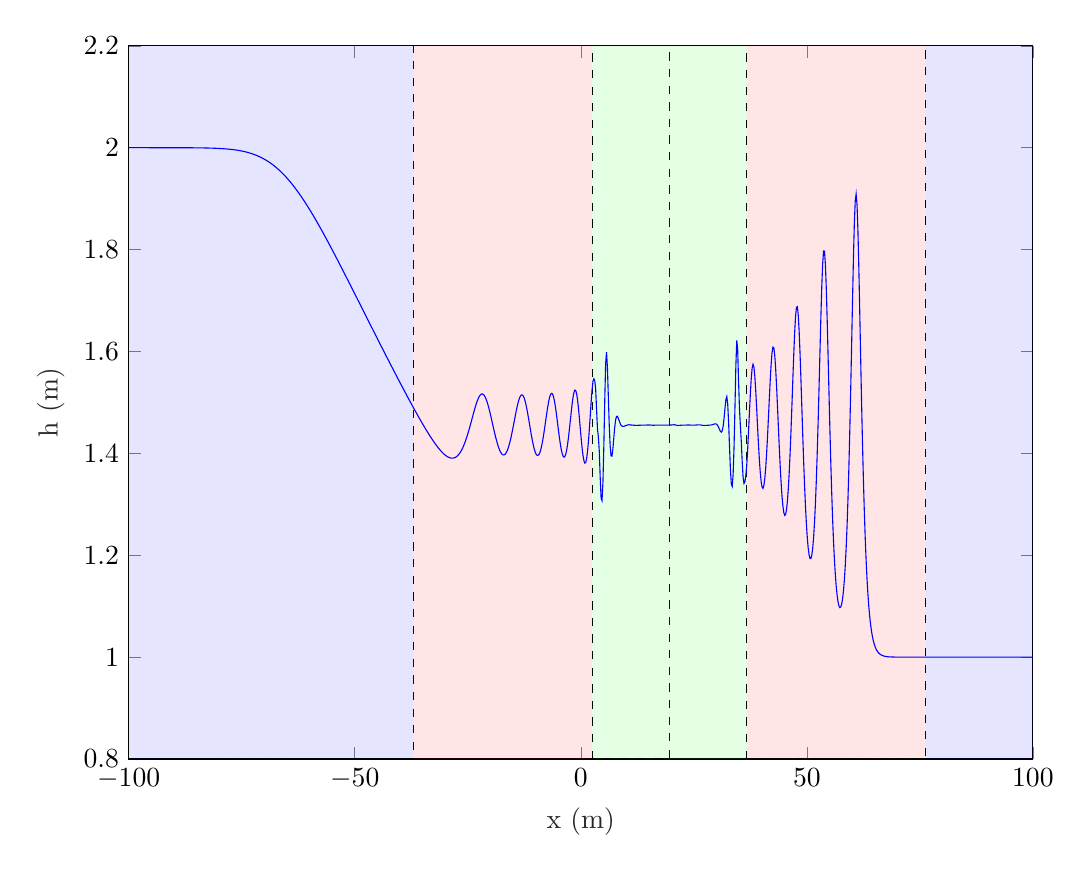
\begin{tikzpicture}

\begin{axis}[%
width=4.521in,
height=3.566in,
at={(0.758in,0.481in)},
scale only axis,
xmin=-100,
xmax=100,
xtick={-100,  -50,    0,   50,  100},
xlabel style={font=\color{white!15!black}},
xlabel={x (m)},
ymin=0.8,
ymax=2.2,
ytick={0.8,   1, 1.2, 1.4, 1.6, 1.8,   2, 2.2},
ylabel style={font=\color{white!15!black}},
ylabel={h (m)},
axis background/.style={fill=white}
]

\addplot[area legend, dashed, draw=black, fill=blue, fill opacity=0.1, forget plot]
table[row sep=crcr] {%
x	y\\
-100	0.8\\
-100	2.2\\
-37.0630892039997	2.2\\
-37.0630892039997	0.8\\
}--cycle;

\addplot[area legend, draw=none, fill=red, fill opacity=0.1, forget plot]
table[row sep=crcr] {%
x	y\\
-37.0630892039997	0.8\\
-37.0630892039997	2.2\\
2.50779195864934	2.2\\
2.50779195864934	0.8\\
}--cycle;

\addplot[area legend, dashed, draw=black, fill=green, fill opacity=0.1, forget plot]
table[row sep=crcr] {%
x	y\\
2.50779195864934	0.8\\
2.50779195864934	2.2\\
19.5890566189392	2.2\\
19.5890566189392	0.8\\
}--cycle;

\addplot[area legend, draw=none, fill=green, fill opacity=0.1, forget plot]
table[row sep=crcr] {%
x	y\\
19.5890566189392	0.8\\
19.5890566189392	2.2\\
36.670321279229	2.2\\
36.670321279229	0.8\\
}--cycle;

\addplot[area legend, dashed, draw=black, fill=red, fill opacity=0.1, forget plot]
table[row sep=crcr] {%
x	y\\
36.670321279229	0.8\\
36.670321279229	2.2\\
76.2412024418781	2.2\\
76.2412024418781	0.8\\
}--cycle;

\addplot[area legend, draw=none, fill=blue, fill opacity=0.1, forget plot]
table[row sep=crcr] {%
x	y\\
76.2412024418781	0.8\\
76.2412024418781	2.2\\
100	2.2\\
100	0.8\\
}--cycle;
\addplot [color=blue, forget plot]
  table[row sep=crcr]{%
-100.1200120012	2\\
-99.9199919991999	1.99999950092733\\
-99.7199719971997	1.99999896308632\\
-99.5199519951995	1.99999866455601\\
-99.3199319931993	1.99999848940598\\
-99.1199119911991	1.99999837441078\\
-98.9198919891989	1.99999828563001\\
-98.7198719871987	1.99999820475942\\
-98.5198519851985	1.9999981218163\\
-98.3198319831983	1.99999803122273\\
-98.1198119811981	1.99999792970955\\
-97.9197919791979	1.99999781519501\\
-97.7197719771977	1.99999768618431\\
-97.5197519751975	1.9999975414474\\
-97.3197319731973	1.99999737984489\\
-97.1197119711971	1.99999720023288\\
-96.9196919691969	1.99999700140929\\
-96.7196719671967	1.99999678208221\\
-96.5196519651965	1.99999654084953\\
-96.3196319631963	1.99999627618424\\
-96.1196119611961	1.99999598642247\\
-95.9195919591959	1.99999566975255\\
-95.7195719571957	1.99999532420429\\
-95.5195519551955	1.9999949476379\\
-95.3195319531953	1.99999453773245\\
-95.1195119511951	1.99999409197348\\
-94.9194919491949	1.9999936076398\\
-94.7194719471947	1.99999308178931\\
-94.5194519451945	1.99999251124385\\
-94.3194319431943	1.99999189257294\\
-94.1194119411941	1.99999122207631\\
-93.9193919391939	1.99999049576529\\
-93.7193719371937	1.9999897093428\\
-93.5193519351935	1.99998885818211\\
-93.3193319331933	1.99998793730399\\
-93.1193119311931	1.99998694135245\\
-92.9192919291929	1.99998586456877\\
-92.7192719271927	1.99998470076389\\
-92.5192519251925	1.99998344328894\\
-92.3192319231923	1.99998208500391\\
-92.1192119211921	1.99998061824425\\
-91.9191919191919	1.99997903478546\\
-91.7191719171917	1.99997732580529\\
-91.5191519151915	1.99997548184373\\
-91.3191319131913	1.99997349276047\\
-91.1191119111911	1.99997134768973\\
-90.9190919091909	1.99996903499243\\
-90.7190719071907	1.99996654220538\\
-90.5190519051905	1.99996385598758\\
-90.3190319031903	1.99996096206323\\
-90.1190119011901	1.99995784516151\\
-89.9189918991899	1.99995448895285\\
-89.7189718971897	1.99995087598158\\
-89.5189518951895	1.99994698759474\\
-89.3189318931893	1.99994280386694\\
-89.1189118911891	1.9999383035211\\
-88.9188918891889	1.99993346384478\\
-88.7188718871887	1.9999282606021\\
-88.5188518851885	1.99992266794088\\
-88.3188318831883	1.99991665829494\\
-88.1188118811881	1.99991020228133\\
-87.9187918791879	1.99990326859228\\
-87.7187718771877	1.99989582388168\\
-87.5187518751875	1.99988783264595\\
-87.3187318731873	1.99987925709907\\
-87.1187118711871	1.99987005704152\\
-86.9186918691869	1.99986018972309\\
-86.7186718671867	1.9998496096992\\
-86.5186518651865	1.99983826868073\\
-86.3186318631863	1.99982611537703\\
-86.1186118611861	1.99981309533203\\
-85.9185918591859	1.99979915075327\\
-85.7185718571857	1.99978422033371\\
-85.5185518551855	1.99976823906616\\
-85.3185318531853	1.9997511380503\\
-85.1185118511851	1.99973284429197\\
-84.9184918491849	1.9997132804949\\
-84.7184718471847	1.99969236484469\\
-84.5184518451845	1.99967001078488\\
-84.3184318431843	1.99964612678535\\
-84.1184118411841	1.99962061610284\\
-83.9183918391839	1.99959337653361\\
-83.7183718371837	1.99956430015859\\
-83.5183518351835	1.99953327308069\\
-83.3183318331833	1.99950017515479\\
-83.1183118311831	1.99946487971041\\
-82.9182918291829	1.99942725326726\\
-82.7182718271827	1.99938715524406\\
-82.5182518251825	1.99934443766084\\
-82.3182318231823	1.99929894483521\\
-82.1182118211821	1.9992505130729\\
-81.9181918191819	1.9991989703532\\
-81.7181718171817	1.99914413600974\\
-81.5181518151815	1.99908582040733\\
-81.3181318131813	1.99902382461557\\
-81.1181118111811	1.9989579400798\\
-80.9180918091809	1.99888794829058\\
-80.7180718071807	1.99881362045227\\
-80.5180518051805	1.99873471715203\\
-80.3180318031803	1.99865098803003\\
-80.1180118011801	1.99856217145234\\
-79.9179917991799	1.99846799418753\\
-79.7179717971797	1.99836817108851\\
-79.5179517951795	1.99826240478089\\
-79.3179317931793	1.99815038535953\\
-79.1179117911791	1.99803179009485\\
-78.9178917891789	1.99790628315056\\
-78.7178717871787	1.99777351531469\\
-78.5178517851785	1.99763312374575\\
-78.3178317831783	1.99748473173598\\
-78.1178117811781	1.99732794849376\\
-77.9177917791779	1.99716236894724\\
-77.7177717771777	1.9969875735714\\
-77.5177517751775	1.99680312824081\\
-77.3177317731773	1.99660858411024\\
-77.1177117711771	1.99640347752565\\
-76.9176917691769	1.99618732996765\\
-76.7176717671767	1.99595964803016\\
-76.5176517651765	1.9957199234363\\
-76.3176317631763	1.99546763309413\\
-76.1176117611761	1.99520223919449\\
-75.9175917591759	1.99492318935332\\
-75.7175717571757	1.99462991680069\\
-75.5175517551755	1.99432184061881\\
-75.3175317531753	1.993998366031\\
-75.1175117511751	1.99365888474381\\
-74.9174917491749	1.99330277534398\\
-74.7174717471747	1.99292940375208\\
-74.5174517451745	1.99253812373436\\
-74.3174317431743	1.99212827747412\\
-74.1174117411741	1.9916991962038\\
-73.9173917391739	1.99125020089869\\
-73.7173717371737	1.99078060303284\\
-73.5173517351735	1.99028970539758\\
-73.3173317331733	1.98977680298278\\
-73.1173117311731	1.98924118392043\\
-72.9172917291729	1.9886821304901\\
-72.7172717271727	1.9880989201852\\
-72.5172517251725	1.98749082683886\\
-72.3172317231723	1.98685712180752\\
-72.1172117211721	1.98619707521036\\
-71.9171917191719	1.98550995722185\\
-71.7171717171717	1.98479503941464\\
-71.5171517151715	1.98405159614943\\
-71.3171317131713	1.98327890600802\\
-71.1171117111711	1.98247625326554\\
-70.9170917091709	1.98164292939717\\
-70.7170717071707	1.98077823461455\\
-70.5170517051705	1.97988147942648\\
-70.3170317031703	1.97895198621843\\
-70.1170117011701	1.97798909084475\\
-69.9169916991699	1.97699214422735\\
-69.7169716971697	1.97596051395448\\
-69.5169516951695	1.97489358587263\\
-69.3169316931693	1.9737907656648\\
-69.1169116911691	1.97265148040797\\
-68.9168916891689	1.97147518010261\\
-68.7168716871687	1.97026133916701\\
-68.5168516851685	1.96900945788907\\
-68.3168316831683	1.96771906382861\\
-68.1168116811681	1.96638971316281\\
-67.9167916791679	1.96502099196807\\
-67.7167716771677	1.96361251743142\\
-67.5167516751675	1.96216393898515\\
-67.3167316731673	1.9606749393584\\
-67.1167116711671	1.95914523553996\\
-66.9166916691669	1.95757457964701\\
-66.7166716671667	1.95596275969472\\
-66.5166516651665	1.95430960026259\\
-66.3166316631663	1.95261496305337\\
-66.1166116611661	1.95087874734156\\
-65.9165916591659	1.94910089030868\\
-65.7165716571657	1.94728136726339\\
-65.5165516551655	1.94542019174504\\
-65.3165316531653	1.94351741550998\\
-65.1165116511651	1.9415731284006\\
-64.9164916491649	1.93958745809778\\
-64.7164716471647	1.93756056975813\\
-64.5164516451645	1.93549266553795\\
-64.3164316431643	1.93338398400652\\
-64.1164116411641	1.93123479945221\\
-63.9163916391639	1.92904542108502\\
-63.7163716371637	1.9268161921401\\
-63.5163516351635	1.9245474888873\\
-63.3163316331633	1.92223971955205\\
-63.1163116311631	1.91989332315347\\
-62.9162916291629	1.91750876826612\\
-62.7162716271627	1.91508655171184\\
-62.5162516251625	1.91262719718868\\
-62.3162316231623	1.91013125384398\\
-62.1162116211621	1.90759929479893\\
-61.9161916191619	1.90503191563203\\
-61.7161716171617	1.90242973282882\\
-61.5161516151615	1.89979338220558\\
-61.3161316131613	1.8971235173141\\
-61.1161116111611	1.89442080783514\\
-60.9160916091609	1.89168593796762\\
-60.7160716071607	1.88891960482041\\
-60.5160516051605	1.88612251681377\\
-60.3160316031603	1.88329539209651\\
-60.1160116011601	1.88043895698534\\
-59.9159915991599	1.87755394443201\\
-59.7159715971597	1.87464109252375\\
-59.5159515951595	1.87170114302209\\
-59.3159315931593	1.86873483994453\\
-59.1159115911591	1.86574292819343\\
-58.9158915891589	1.8627261522358\\
-58.7158715871587	1.85968525483725\\
-58.5158515851585	1.85662097585315\\
-58.3158315831583	1.85353405107925\\
-58.1158115811581	1.85042521116383\\
-57.9157915791579	1.84729518058306\\
-57.7157715771577	1.84414467668051\\
-57.5157515751575	1.84097440877184\\
-57.3157315731573	1.83778507731478\\
-57.1157115711571	1.8345773731447\\
-56.9156915691569	1.83135197677511\\
-56.7156715671567	1.82810955776284\\
-56.5156515651565	1.82485077413667\\
-56.3156315631563	1.82157627188823\\
-56.1156115611561	1.81828668452392\\
-55.9155915591559	1.81498263267596\\
-55.7155715571557	1.81166472377076\\
-55.5155515551555	1.80833355175268\\
-55.3155315531553	1.80498969686079\\
-55.1155115511551	1.80163372545651\\
-54.9154915491549	1.79826618989966\\
-54.7154715471547	1.79488762847039\\
-54.5154515451545	1.79149856533449\\
-54.3154315431543	1.78809951054955\\
-54.1154115411541	1.78469096010931\\
-53.9153915391539	1.78127339602365\\
-53.7153715371537	1.77784728643166\\
-53.5153515351535	1.77441308574526\\
-53.3153315331533	1.77097123482074\\
-53.1153115311531	1.7675221611561\\
-52.9152915291529	1.76406627911142\\
-52.7152715271527	1.76060399015037\\
-52.5152515251525	1.75713568310031\\
-52.3152315231523	1.75366173442911\\
-52.1152115211521	1.75018250853658\\
-51.9151915191519	1.74669835805863\\
-51.7151715171517	1.74320962418228\\
-51.5151515151515	1.73971663696994\\
-51.3151315131513	1.73621971569131\\
-51.1151115111511	1.7327191691614\\
-50.9150915091509	1.72921529608336\\
-50.7150715071507	1.72570838539486\\
-50.5150515051505	1.72219871661676\\
-50.3150315031503	1.71868656020328\\
-50.1150115011501	1.7151721778924\\
-49.9149914991499	1.711655823056\\
-49.7149714971497	1.70813774104872\\
-49.5149514951495	1.70461816955506\\
-49.3149314931493	1.7010973389342\\
-49.1149114911491	1.69757547256195\\
-48.9148914891489	1.69405278716956\\
-48.7148714871487	1.69052949317909\\
-48.5148514851485	1.68700579503515\\
-48.3148314831483	1.68348189153281\\
-48.1148114811481	1.67995797614172\\
-47.9147914791479	1.67643423732635\\
-47.7147714771477	1.67291085886256\\
-47.5147514751475	1.66938802015051\\
-47.3147314731473	1.66586589652419\\
-47.1147114711471	1.66234465955784\\
-46.9146914691469	1.65882447736956\\
-46.7146714671467	1.65530551492252\\
-46.5146514651465	1.65178793432414\\
-46.3146314631463	1.64827189512384\\
-46.1146114611461	1.64475755460984\\
-45.9145914591459	1.64124506810555\\
-45.7145714571457	1.63773458926636\\
-45.5145514551455	1.63422627037743\\
-45.3145314531453	1.63072026265327\\
-45.1145114511451	1.6272167165399\\
-44.9144914491449	1.62371578202064\\
-44.7144714471447	1.62021760892626\\
-44.5144514451445	1.61672234725067\\
-44.3144314431443	1.61323014747318\\
-44.1144114411441	1.6097411608886\\
-43.9143914391439	1.60625553994623\\
-43.7143714371437	1.60277343859934\\
-43.5143514351435	1.59929501266641\\
-43.3143314331433	1.59582042020576\\
-43.1143114311431	1.59234982190518\\
-42.9142914291429	1.58888338148843\\
-42.7142714271427	1.58542126614046\\
-42.5142514251425	1.58196364695346\\
-42.3142314231423	1.57851069939605\\
-42.1142114211421	1.57506260380783\\
-41.9141914191419	1.57161954592219\\
-41.7141714171417	1.56818171741997\\
-41.5141514151415	1.56474931651712\\
-41.3141314131413	1.56132254858979\\
-41.1141114111411	1.55790162684027\\
-40.9140914091409	1.55448677300784\\
-40.7140714071407	1.55107821812882\\
-40.5140514051405	1.54767620335029\\
-40.3140314031403	1.54428098080276\\
-40.1140114011401	1.54089281453708\\
-39.9139913991399	1.53751198153182\\
-39.7139713971397	1.53413877277744\\
-39.5139513951395	1.53077349444464\\
-39.3139313931393	1.52741646914442\\
-39.1139113911391	1.52406803728867\\
-38.9138913891389	1.5207285585604\\
-38.7138713871387	1.51739841350387\\
-38.5138513851385	1.51407800524572\\
-38.3138313831383	1.51076776135929\\
-38.1138113811381	1.50746813588544\\
-37.9137913791379	1.50417961152435\\
-37.7137713771377	1.50090270201421\\
-37.5137513751375	1.49763795471419\\
-37.3137313731373	1.49438595341064\\
-37.1137113711371	1.49114732136716\\
-36.9136913691369	1.48792272464124\\
-36.7136713671367	1.48471287569211\\
-36.5136513651365	1.48151853730658\\
-36.3136313631363	1.47834052687222\\
-36.1136113611361	1.47517972102972\\
-35.9135913591359	1.47203706073897\\
-35.7135713571357	1.46891355679641\\
-35.5135513551355	1.46581029584423\\
-35.3135313531353	1.46272844691548\\
-35.1135113511351	1.45966926856234\\
-34.9134913491349	1.45663411661857\\
-34.7134713471347	1.45362445265069\\
-34.5134513451345	1.45064185315629\\
-34.3134313431343	1.44768801957157\\
-34.1134113411341	1.44476478915359\\
-33.9133913391339	1.4418741468063\\
-33.7133713371337	1.43901823792247\\
-33.5133513351335	1.43619938231574\\
-33.3133313331333	1.43342008931886\\
-33.1133113311331	1.43068307412477\\
-32.9132913291329	1.42799127544586\\
-32.7132713271327	1.42534787456406\\
-32.5132513251325	1.42275631583879\\
-32.3132313231323	1.42022032873104\\
-32.1132113211321	1.41774395138905\\
-31.9131913191319	1.41533155582274\\
-31.7131713171317	1.41298787467029\\
-31.5131513151315	1.41071802952708\\
-31.3131313131313	1.40852756076593\\
-31.1131113111311	1.40642245872337\\
-30.9130913091309	1.40440919605891\\
-30.7130713071307	1.40249476100919\\
-30.5130513051305	1.40068669115338\\
-30.3130313031303	1.39899310717688\\
-30.1130113011301	1.39742274596279\\
-29.9129912991299	1.39598499214999\\
-29.7129712971297	1.39468990706882\\
-29.5129512951295	1.39354825369456\\
-29.3129312931293	1.39257151593996\\
-29.1129112911291	1.39177191023706\\
-28.9128912891289	1.39116238693059\\
-28.7128712871287	1.39075661851861\\
-28.5128512851285	1.3905689660827\\
-28.3128312831283	1.39061457493451\\
-28.1128112811281	1.3909089255804\\
-27.9127912791279	1.39146803711155\\
-27.7127712771277	1.39230827428596\\
-27.5127512751275	1.39344613120957\\
-27.3127312731273	1.39489801995333\\
-27.1127112711271	1.39667992364866\\
-26.9126912691269	1.39880707950477\\
-26.7126712671267	1.40129352960032\\
-26.5126512651265	1.40415156784694\\
-26.3126312631263	1.40739119269163\\
-26.1126112611261	1.4110193665671\\
-25.9125912591259	1.41503922993595\\
-25.7125712571257	1.41944928383902\\
-25.5125512551255	1.42424238080916\\
-25.3125312531253	1.42940477137978\\
-25.1125112511251	1.43491510524948\\
-24.9124912491249	1.44074337493801\\
-24.7124712471247	1.44685005224975\\
-24.5124512451245	1.45318526649364\\
-24.3124312431243	1.45968823293254\\
-24.1124112411241	1.46628698077278\\
-23.9123912391239	1.47289849900344\\
-23.7123712371237	1.47942930197073\\
-23.5123512351235	1.48577663392502\\
-23.3123312331233	1.49183028651852\\
-23.1123112311231	1.49747500411395\\
-22.9122912291229	1.50259362356516\\
-22.7122712271227	1.50707072756168\\
-22.5122512251225	1.51079668887714\\
-22.3122312231223	1.51367203638528\\
-22.1122112211221	1.5156117156728\\
-21.9121912191219	1.51654905310722\\
-21.7121712171217	1.51643907969443\\
-21.5121512151215	1.51526183103799\\
-21.3121312131213	1.5130230983142\\
-21.1121112111211	1.50975492693953\\
-20.9120912091209	1.50551485151855\\
-20.7120712071207	1.5003838960842\\
-20.5120512051205	1.49446350640095\\
-20.3120312031203	1.48787189567957\\
-20.1120112011201	1.48073994496669\\
-19.9119911991199	1.47320687417978\\
-19.7119711971197	1.46541602373747\\
-19.5119511951195	1.45751105094492\\
-19.3119311931193	1.44963266732225\\
-19.1119111911191	1.44191595170203\\
-18.9118911891189	1.43448829537956\\
-18.7118711871187	1.42746802464366\\
-18.5118511851185	1.4209636050717\\
-18.3118311831183	1.41507331980976\\
-18.1118111811181	1.40988528123492\\
-17.9117911791179	1.40547767953464\\
-17.7117711771177	1.40191912966596\\
-17.5117511751175	1.39926900492101\\
-17.3117311731173	1.39757760895913\\
-17.1117111711171	1.39688429139296\\
-16.9116911691169	1.39722647515201\\
-16.7116711671167	1.39861931981814\\
-16.5116511651165	1.40107403438673\\
-16.3116311631163	1.40458641003825\\
-16.1116111611161	1.40913642113233\\
-15.9115911591159	1.41468545032929\\
-15.7115711571157	1.42117326596033\\
-15.5115511551155	1.42851487725013\\
-15.3115311531153	1.4365975944688\\
-15.1115111511151	1.44527847806394\\
-14.9114911491149	1.45438276473766\\
-14.7114711471147	1.46370386872913\\
-14.5114511451145	1.47300521989781\\
-14.3114311431143	1.48202468068253\\
-14.1114111411141	1.4904818512355\\
-13.9113911391139	1.49808830731171\\
-13.7113711371137	1.50456068960722\\
-13.5113511351135	1.50963587953516\\
-13.3113311331133	1.51308723559047\\
-13.1113111311131	1.51474014403958\\
-12.9112911291129	1.51448531758543\\
-12.7112711271127	1.51229086053232\\
-12.5112511251125	1.50820422011802\\
-12.3112311231123	1.50235230909853\\
-12.1112111211121	1.49493483493154\\
-11.9111911191119	1.48621256889159\\
-11.7111711171117	1.47649322584471\\
-11.5111511151115	1.46611460897952\\
-11.3111311131113	1.45542844095852\\
-11.1111111111111	1.44478580942741\\
-10.9110911091109	1.43452468205384\\
-10.7110711071107	1.42496037072912\\
-10.5110511051105	1.41637891914392\\
-10.3110311031103	1.40903292494401\\
-10.1110111011101	1.40313919088828\\
-9.91099109910991	1.39887761357129\\
-9.71097109710971	1.39639045141289\\
-9.5109510951095	1.3957844265317\\
-9.3109310931093	1.39711339742929\\
-9.1109110911091	1.40040348470073\\
-8.9108910891089	1.40562064691021\\
-8.7108710871087	1.4126778184992\\
-8.51085108510851	1.42142450314662\\
-8.31083108310831	1.43163895658816\\
-8.11081108110811	1.44302133571646\\
-7.91079107910791	1.45518979746287\\
-7.71077107710771	1.46768170236583\\
-7.51075107510751	1.47996236380442\\
-7.31073107310731	1.49144365929059\\
-7.1107110711071	1.50151396307193\\
-6.9106910691069	1.50957854824756\\
-6.7106710671067	1.51510851002079\\
-6.5106510651065	1.51769281301356\\
-6.3106310631063	1.51707729445229\\
-6.11061106110611	1.51321785349944\\
-5.91059105910591	1.50627281742691\\
-5.71057105710571	1.49660385432861\\
-5.51055105510551	1.48474415850392\\
-5.31053105310531	1.47135321589488\\
-5.11051105110511	1.4571641620341\\
-4.91049104910491	1.4429321524224\\
-4.7104710471047	1.42938987964094\\
-4.5104510451045	1.41721300307546\\
-4.3104310431043	1.40699736455477\\
-4.1104110411041	1.3992439917419\\
-3.9103910391039	1.39435083243218\\
-3.71037103710371	1.39260464262582\\
-3.51035103510351	1.39418940944172\\
-3.31033103310331	1.39914104077392\\
-3.11031103110311	1.40736925090253\\
-2.91029102910291	1.41861899285776\\
-2.71027102710271	1.43245101342906\\
-2.51025102510251	1.44822074057783\\
-2.3102310231023	1.46506655451811\\
-2.1102110211021	1.48191888350632\\
-1.9101910191019	1.49754207118168\\
-1.7101710171017	1.51061878227216\\
-1.5101510151015	1.51988110547336\\
-1.31013101310131	1.52427954201963\\
-1.11011101110111	1.52312647303146\\
-0.91009100910091	1.51630236428631\\
-0.710071007100709	1.50423603405536\\
-0.510051005100507	1.48790058563379\\
-0.310031003100306	1.4686799507291\\
-0.110011001100105	1.44819485944954\\
0.0900090009000962	1.42812484466475\\
0.290029002900297	1.41006348165341\\
0.490049004900499	1.39541759598036\\
0.6900690069007	1.38535026145926\\
0.890089008900901	1.3807462195281\\
1.09010901090109	1.38222466480084\\
1.29012901290129	1.39002760496606\\
1.49014901490149	1.40404733831749\\
1.69016901690169	1.42370267998915\\
1.89018901890189	1.44783441771924\\
2.09020902090209	1.47458338326238\\
2.2902290229023	1.50132003977679\\
2.4902490249025	1.52491191926622\\
2.6902690269027	1.54156454428223\\
2.8902890289029	1.54642665800627\\
3.0903090309031	1.54237452465847\\
3.2903290329033	1.52551270662569\\
3.4903490349035	1.48487380873849\\
3.69036903690369	1.44778480952842\\
3.89038903890389	1.43154422467913\\
4.09040904090409	1.4030713617025\\
4.29042904290429	1.35184494230331\\
4.49044904490449	1.31201714541919\\
4.6904690469047	1.30722003726545\\
4.8904890489049	1.3426002598265\\
5.0905090509051	1.41307701346819\\
5.2905290529053	1.50207844791207\\
5.4905490549055	1.57648742052323\\
5.6905690569057	1.59868942348001\\
5.8905890589059	1.56742471065623\\
6.09060906090609	1.51020077913597\\
6.29062906290629	1.45442669586424\\
6.49064906490649	1.41445427236947\\
6.69066906690669	1.39492733061817\\
6.89068906890689	1.39454522630394\\
7.0907090709071	1.40835791397949\\
7.2907290729073	1.42938573960437\\
7.4907490749075	1.45017863059563\\
7.6907690769077	1.46516851245064\\
7.8907890789079	1.47229213408864\\
8.0908090809081	1.47277805804732\\
8.2908290829083	1.46907699597859\\
8.49084908490849	1.46382025914771\\
8.69086908690869	1.45901891120216\\
8.89088908890889	1.45552545336532\\
9.09090909090909	1.45356251061693\\
9.29092909290929	1.45286365013244\\
9.4909490949095	1.45300887225311\\
9.6909690969097	1.45360656803275\\
9.8909890989099	1.45434488957776\\
10.0910091009101	1.45500131807467\\
10.2910291029103	1.45552828550359\\
10.4910491049105	1.45596062339078\\
10.6910691069107	1.45615395078531\\
10.8910891089109	1.45591463570006\\
11.0911091109111	1.45562659180956\\
11.2911291129113	1.45557243934361\\
11.4911491149115	1.45542734360368\\
11.6911691169117	1.45523105336008\\
11.8911891189119	1.45508775026456\\
12.0912091209121	1.45500372772503\\
12.2912291229123	1.45498007272372\\
12.4912491249125	1.45500836942596\\
12.6912691269127	1.45507568172372\\
12.8912891289129	1.45516028102107\\
13.0913091309131	1.45523313681441\\
13.2913291329133	1.45528509055348\\
13.4913491349135	1.45533288725628\\
13.6913691369137	1.45536395913297\\
13.8913891389139	1.45541465054792\\
14.0914091409141	1.4554673317141\\
14.2914291429143	1.45547993768375\\
14.4914491449145	1.45551655311873\\
14.6914691469147	1.45561200175496\\
14.8914891489149	1.45573424815264\\
15.0915091509151	1.45576344508366\\
15.2915291529153	1.45564807648876\\
15.4915491549155	1.45545605408599\\
15.6915691569157	1.45529922466869\\
15.8915891589159	1.45524167976987\\
16.0916091609161	1.45522626432073\\
16.2916291629163	1.45524377993837\\
16.4916491649165	1.45539343543431\\
16.6916691669167	1.45554429585994\\
16.8916891689169	1.45554261057587\\
17.0917091709171	1.45551740046874\\
17.2917291729173	1.45548985114544\\
17.4917491749175	1.45546554533378\\
17.6917691769177	1.45546414837133\\
17.8917891789179	1.4554710160197\\
18.0918091809181	1.45547684079071\\
18.2918291829183	1.45546077075719\\
18.4918491849185	1.45540778480355\\
18.6918691869187	1.45534841944975\\
18.8918891889189	1.45533038036821\\
19.0919091909191	1.45536230056509\\
19.2919291929193	1.45541025975063\\
19.4919491949195	1.45545289464914\\
19.6919691969197	1.45550901703382\\
19.8919891989199	1.45560451680553\\
20.0920092009201	1.45573746811342\\
20.2920292029203	1.45592913882229\\
20.4920492049205	1.45611442122753\\
20.6920692069207	1.45611525220327\\
20.8920892089209	1.45584048571175\\
21.0921092109211	1.45538913537894\\
21.2921292129213	1.45497847066885\\
21.4921492149215	1.4547948318947\\
21.6921692169217	1.45485359229608\\
21.8921892189219	1.45500901276755\\
22.0922092209221	1.4551363285858\\
22.2922292229223	1.45525547695787\\
22.4922492249225	1.45537998094536\\
22.6922692269227	1.45544505912965\\
22.8922892289229	1.4554688781373\\
23.0923092309231	1.45549845555842\\
23.2923292329233	1.45553055351336\\
23.4923492349235	1.4555761080189\\
23.6923692369237	1.45563090578376\\
23.8923892389239	1.45564232655067\\
24.0924092409241	1.45558631877258\\
24.2924292429243	1.45549343124201\\
24.4924492449245	1.45540083662468\\
24.6924692469247	1.45533279284321\\
24.8924892489249	1.45532995412647\\
25.0925092509251	1.45539079853218\\
25.2925292529253	1.45549494109034\\
25.4925492549255	1.45561365289943\\
25.6925692569257	1.45572360252783\\
25.8925892589259	1.45586010189638\\
26.0926092609261	1.45599589803344\\
26.2926292629263	1.45600285301601\\
26.4926492649265	1.45579809560654\\
26.6926692669267	1.45542275664451\\
26.8926892689269	1.45503444516378\\
27.0927092709271	1.45479985897316\\
27.2927292729273	1.45477273506505\\
27.4927492749275	1.45486980778665\\
27.6927692769277	1.45496029559467\\
27.8927892789279	1.45501655998384\\
28.0928092809281	1.45510357475734\\
28.2928292829283	1.45523463345766\\
28.4928492849285	1.45537241711965\\
28.6928692869287	1.45554643619197\\
28.8928892889289	1.45584600514722\\
29.0929092909291	1.45630728807539\\
29.2929292929293	1.45688370794517\\
29.4929492949295	1.4574839889347\\
29.6929692969297	1.45791107281226\\
29.8929892989299	1.45779312811513\\
30.0930093009301	1.45672190696912\\
30.2930293029303	1.45441519114916\\
30.4930493049305	1.45087354467921\\
30.6930693069307	1.44662674263775\\
30.8930893089309	1.44292691196857\\
31.0931093109311	1.44159770252286\\
31.2931293129313	1.44477737758383\\
31.4931493149315	1.45406300745419\\
31.6931693169317	1.46957605678406\\
31.8931893189319	1.48895292578166\\
32.0932093209321	1.506068225298\\
32.2932293229323	1.51148623484825\\
32.4932493249325	1.49655878142507\\
32.6932693269327	1.46057040954931\\
32.8932893289329	1.41285981624429\\
33.0933093309331	1.36816574916297\\
33.2933293329333	1.33945764569469\\
33.4933493349335	1.33503078442236\\
33.6933693369337	1.35935189383838\\
33.8933893389339	1.41249046295992\\
34.0934093409341	1.48880665209869\\
34.2934293429343	1.57098196894304\\
34.4934493449345	1.6217505798928\\
34.6934693469347	1.6043533227473\\
34.8934893489349	1.54173827297502\\
35.0935093509351	1.48749588285881\\
35.2935293529353	1.45434683179171\\
35.4935493549355	1.42364961433921\\
35.6935693569357	1.38417783551091\\
35.8935893589359	1.35296980862965\\
36.0936093609361	1.34082853096418\\
36.2936293629363	1.34413670598739\\
36.4936493649365	1.35628634338893\\
36.6936693669367	1.37631864457075\\
36.8936893689369	1.40550741907328\\
37.0937093709371	1.44129138749262\\
37.2937293729373	1.47936120719399\\
37.4937493749375	1.51583561323681\\
37.6937693769377	1.54647043074194\\
37.8937893789379	1.56712988101855\\
38.0938093809381	1.57491315139729\\
38.2938293829383	1.56902722991562\\
38.4938493849385	1.55057143722288\\
38.6938693869387	1.52255082166367\\
38.8938893889389	1.48872318377193\\
39.0939093909391	1.45287535497477\\
39.2939293929393	1.41829547485863\\
39.4939493949395	1.38755173538642\\
39.6939693969397	1.36248634319897\\
39.8939893989399	1.34432041005876\\
40.0940094009401	1.33378989786357\\
40.2940294029403	1.33123909966405\\
40.4940494049405	1.33683472134777\\
40.6940694069407	1.35032866913803\\
40.8940894089409	1.37129914402551\\
41.0941094109411	1.3989575221955\\
41.2941294129413	1.43207363661986\\
41.4941494149415	1.46886908239298\\
41.6941694169417	1.50694415517736\\
41.8941894189419	1.54330025580432\\
42.0942094209421	1.57453057540102\\
42.2942294229423	1.59723036520903\\
42.4942494249425	1.6085960156076\\
42.6942694269427	1.60706701267132\\
42.8942894289429	1.59266262308213\\
43.0943094309431	1.5670560667954\\
43.2943294329433	1.53304078773409\\
43.4943494349435	1.4939132847479\\
43.6943694369437	1.45290369589136\\
43.8943894389439	1.41280440438936\\
44.0944094409441	1.37581256312414\\
44.2944294429443	1.34353024839811\\
44.4944494449445	1.31705170322676\\
44.6944694469447	1.29708642005523\\
44.8944894489449	1.28407905764835\\
45.0945094509451	1.27831356553572\\
45.2945294529453	1.27996510643821\\
45.4945494549455	1.28917383440147\\
45.6945694569457	1.30600171280181\\
45.8945894589459	1.33041301590117\\
46.0946094609461	1.36218845999164\\
46.2946294629463	1.40079989713712\\
46.4946494649465	1.44524927102977\\
46.6946694669467	1.49388759002904\\
46.8946894689469	1.54424768992527\\
47.0947094709471	1.59296535283755\\
47.2947294729473	1.63588976410372\\
47.4947494749475	1.66850714883405\\
47.6947694769477	1.68672854016134\\
47.8947894789479	1.68789617771437\\
48.0948094809481	1.67148520407385\\
48.2948294829483	1.63942363961356\\
48.4948494849485	1.59536337668195\\
48.6948694869487	1.54372940735492\\
48.8948894889489	1.4888248619933\\
49.0949094909491	1.43426491207977\\
49.2949294929493	1.3827663566208\\
49.4949494949495	1.33616812262392\\
49.6949694969497	1.29558377869046\\
49.8949894989499	1.26158863066247\\
50.0950095009501	1.23440297883415\\
50.2950295029503	1.21404850280144\\
50.4950495049505	1.20046736176467\\
50.6950695069507	1.19361361521808\\
50.8950895089509	1.19350758103226\\
51.0951095109511	1.2002734756566\\
51.2951295129513	1.21414502825543\\
51.4951495149515	1.23544976217285\\
51.6951695169517	1.26456123230077\\
51.8951895189519	1.30181877401937\\
52.0952095209521	1.3473943359004\\
52.2952295229523	1.40111027415293\\
52.4952495249525	1.4621850870835\\
52.6952695269527	1.52893398810256\\
52.8952895289529	1.59843291889739\\
53.0953095309531	1.66626890729136\\
53.2953295329533	1.72652752181175\\
53.4953495349535	1.77234262434547\\
53.6953695369537	1.79722800511857\\
53.8953895389539	1.79703476091182\\
54.0954095409541	1.77143650299595\\
54.2954295429543	1.72426058528841\\
54.4954495449545	1.66184903527027\\
54.6954695469547	1.59108895540749\\
54.8954895489549	1.51799640507659\\
55.0955095509551	1.44709785759185\\
55.2955295529553	1.38137528232199\\
55.4955495549555	1.32252455755421\\
55.6955695569557	1.27126418437972\\
55.8955895589559	1.22766624977511\\
56.0956095609561	1.19139377354625\\
56.2956295629563	1.16191321968194\\
56.4956495649565	1.13861686301141\\
56.6956695669567	1.12092576641959\\
56.8956895689569	1.10834713221286\\
57.0957095709571	1.10050432390338\\
57.2957295729573	1.0971758467348\\
57.4957495749575	1.09827746992442\\
57.6957695769577	1.10391324037285\\
57.8957895789579	1.11433866847464\\
58.0958095809581	1.12998182056814\\
58.2958295829583	1.15143414682388\\
58.4958495849585	1.17941898013044\\
58.6958695869587	1.21477111654413\\
58.8958895889589	1.25834095930976\\
59.0959095909591	1.31089820453224\\
59.2959295929593	1.3729261366802\\
59.4959495949595	1.44436574998947\\
59.6959695969597	1.52423232059236\\
59.8959895989599	1.61015107450194\\
60.0960096009601	1.69782734908871\\
60.2960296029603	1.78064200262217\\
60.4960496049605	1.84972848390275\\
60.6960696069607	1.89522038201315\\
60.8960896089609	1.90909040169856\\
61.0961096109611	1.88839459590092\\
61.2961296129613	1.83703382673749\\
61.4961496149615	1.7637191272341\\
61.6961696169617	1.67830737118676\\
61.8961896189619	1.58931343928796\\
62.0962096209621	1.50291978005624\\
62.2962296229623	1.42301627009727\\
62.4962496249625	1.35165166594659\\
62.6962696269627	1.28955509013115\\
62.8962896289629	1.23659144493208\\
63.0963096309631	1.19211370698623\\
63.2963296329633	1.15521500060792\\
63.4963496349635	1.12489722198272\\
63.6963696369637	1.10017593372213\\
63.8963896389639	1.08013964037291\\
64.0964096409641	1.06397825230914\\
64.2964296429643	1.05099194837806\\
64.4964496449645	1.04058842678606\\
64.6964696469647	1.03227394413554\\
64.8964896489649	1.02564160854173\\
65.0965096509651	1.02035902825395\\
65.2965296529653	1.01615649969221\\
65.4965496549655	1.01281632888374\\
65.6965696569657	1.01016351835186\\
65.8965896589659	1.00805784164784\\
66.0966096609661	1.00638721545258\\
66.2966296629663	1.00506222715321\\
66.4966496649665	1.0040116593287\\
66.6966696669667	1.00317885586178\\
66.8966896689669	1.00251878765374\\
67.0967096709671	1.00199569331502\\
67.2967296729673	1.00158118841203\\
67.4967496749675	1.00125275410129\\
67.6967696769677	1.00099253144504\\
67.8967896789679	1.00078636109042\\
68.0968096809681	1.00062301931883\\
68.2968296829683	1.00049361089648\\
68.4968496849685	1.00039108690708\\
68.6968696869687	1.00030986206573\\
68.8968896889689	1.00024551112983\\
69.0969096909691	1.00019452814554\\
69.2969296929693	1.00015413557841\\
69.4969496949695	1.00012213302517\\
69.6969696969697	1.00009677731875\\
69.8969896989699	1.00007668752478\\
70.0970097009701	1.00006076966882\\
70.2970297029703	1.00004815710122\\
70.4970497049705	1.00003816325328\\
70.6970697069707	1.00003024421138\\
70.8970897089709	1.00002396906958\\
71.0971097109711	1.00001899644433\\
71.2971297129713	1.00001505587066\\
71.4971497149715	1.00001193306517\\
71.6971697169717	1.00000945825222\\
71.8971897189719	1.00000749691631\\
72.0972097209721	1.00000594247651\\
72.2972297229723	1.00000471048326\\
72.4972497249725	1.00000373402114\\
72.6972697269727	1.00000296006693\\
72.8972897289729	1.00000234660434\\
73.0973097309731	1.00000186033826\\
73.2973297329733	1.00000147488378\\
73.4973497349735	1.00000116933147\\
73.6973697369737	1.00000092711061\\
73.8973897389739	1.00000073508856\\
74.0974097409741	1.0000005828571\\
74.2974297429743	1.00000046216702\\
74.4974497449745	1.00000036648006\\
74.6974697469747	1.00000029061391\\
74.8974897489749	1.00000023046088\\
75.0975097509751	1.00000018276494\\
75.2975297529753	1.0000001449451\\
75.4975497549755	1.00000011495537\\
75.6975697569757	1.00000009117382\\
75.8975897589759	1.00000007231465\\
76.0976097609761	1.00000005735851\\
76.2976297629763	1.00000004549721\\
76.4976497649765	1.00000003609003\\
76.6976697669767	1.00000002862895\\
76.8976897689769	1.00000002271115\\
77.0977097709771	1.00000001801726\\
77.2977297729773	1.00000001429401\\
77.4977497749775	1.00000001134058\\
77.6977697769777	1.00000000899773\\
77.8977897789779	1.00000000713914\\
78.0978097809781	1.00000000566468\\
78.2978297829783	1.00000000449491\\
78.4978497849785	1.00000000356683\\
78.6978697869787	1.00000000283048\\
78.8978897889789	1.00000000224623\\
79.0979097909791	1.00000000178264\\
79.2979297929793	1.00000000141478\\
79.4979497949795	1.00000000112288\\
79.6979697969797	1.00000000089123\\
79.8979897989799	1.0000000007074\\
80.0980098009801	1.00000000056151\\
80.2980298029803	1.00000000044572\\
80.4980498049805	1.00000000035382\\
80.6980698069807	1.00000000028088\\
80.8980898089809	1.00000000022299\\
81.0981098109811	1.00000000017703\\
81.2981298129813	1.00000000014055\\
81.4981498149815	1.00000000011159\\
81.6981698169817	1.0000000000886\\
81.8981898189819	1.00000000007035\\
82.0982098209821	1.00000000005586\\
82.2982298229823	1.00000000004436\\
82.4982498249825	1.00000000003522\\
82.6982698269827	1.00000000002797\\
82.8982898289829	1.00000000002221\\
83.0983098309831	1.00000000001764\\
83.2983298329833	1.00000000001401\\
83.4983498349835	1.00000000001112\\
83.6983698369837	1.00000000000883\\
83.8983898389839	1.00000000000702\\
84.0984098409841	1.00000000000557\\
84.2984298429843	1.00000000000442\\
84.4984498449845	1.00000000000351\\
84.6984698469847	1.00000000000279\\
84.8984898489849	1.00000000000221\\
85.0985098509851	1.00000000000176\\
85.2985298529853	1.00000000000139\\
85.4985498549855	1.00000000000111\\
85.6985698569857	1.00000000000088\\
85.8985898589859	1.0000000000007\\
86.0986098609861	1.00000000000055\\
86.2986298629863	1.00000000000043\\
86.4986498649865	1.00000000000034\\
86.6986698669867	1.00000000000027\\
86.8986898689869	1.00000000000021\\
87.0987098709871	1.00000000000017\\
87.2987298729873	1.00000000000013\\
87.4987498749875	1.0000000000001\\
87.6987698769877	1.00000000000008\\
87.8987898789879	1.00000000000006\\
88.0988098809881	1.00000000000004\\
88.2988298829883	1.00000000000003\\
88.4988498849885	1.00000000000002\\
88.6988698869887	1.00000000000002\\
88.8988898889889	1.00000000000001\\
89.0989098909891	1.00000000000001\\
89.2989298929893	1\\
89.4989498949895	1\\
89.6989698969897	1\\
89.8989898989899	1\\
90.0990099009901	1\\
90.2990299029903	1\\
90.4990499049905	1\\
90.6990699069907	1\\
90.8990899089909	1\\
91.0991099109911	1\\
91.2991299129913	1\\
91.4991499149915	1\\
91.6991699169917	1\\
91.8991899189919	1\\
92.0992099209921	1\\
92.2992299229923	1\\
92.4992499249925	1\\
92.6992699269927	1\\
92.8992899289929	1\\
93.0993099309931	1\\
93.2993299329933	1\\
93.4993499349935	1\\
93.6993699369937	1\\
93.8993899389939	1\\
94.0994099409941	1\\
94.2994299429943	1\\
94.4994499449945	1\\
94.6994699469947	1\\
94.8994899489949	1\\
95.0995099509951	1\\
95.2995299529953	1\\
95.4995499549955	1\\
95.6995699569957	1\\
95.8995899589959	1\\
96.0996099609961	1\\
96.2996299629963	1\\
96.4996499649965	1\\
96.6996699669967	1\\
96.8996899689969	1\\
97.0997099709971	1\\
97.2997299729973	1\\
97.4997499749975	1\\
97.6997699769977	1\\
97.8997899789979	1\\
98.0998099809981	1\\
98.2998299829983	1\\
98.4998499849985	1\\
98.6998699869987	1\\
98.8998899889989	1\\
99.0999099909991	1\\
99.2999299929993	1\\
99.4999499949995	1\\
99.6999699969997	1\\
99.8999899989999	1\\
100.100010001	1\\
};
\end{axis}
\end{tikzpicture}%
		\caption{$h$}
	\end{subfigure}
	\begin{subfigure}{0.49\textwidth}
		\centering
		% This file was created by matlab2tikz.
%
%The latest updates can be retrieved from
%  http://www.mathworks.com/matlabcentral/fileexchange/22022-matlab2tikz-matlab2tikz
%where you can also make suggestions and rate matlab2tikz.
%
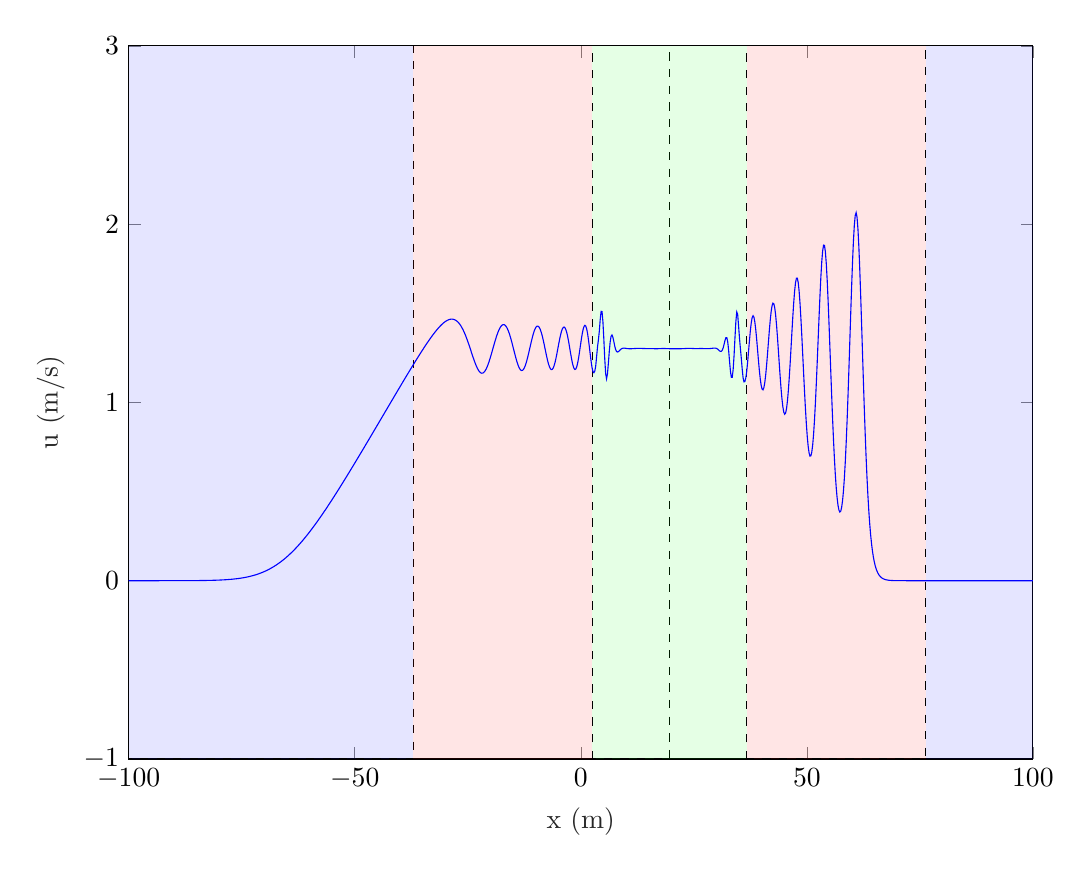
\begin{tikzpicture}

\begin{axis}[%
width=4.521in,
height=3.566in,
at={(0.758in,0.481in)},
scale only axis,
xmin=-100,
xmax=100,
xtick={-100,  -50,    0,   50,  100},
xlabel style={font=\color{white!15!black}},
xlabel={x (m)},
ymin=-1,
ymax=3,
ytick={-1,  0,  1,  2,  3},
ylabel style={font=\color{white!15!black}},
ylabel={u (m/s)},
axis background/.style={fill=white}
]

\addplot[area legend, dashed, draw=black, fill=blue, fill opacity=0.1, forget plot]
table[row sep=crcr] {%
x	y\\
-100	-1\\
-100	3\\
-37.0630892039997	3\\
-37.0630892039997	-1\\
}--cycle;

\addplot[area legend, draw=none, fill=red, fill opacity=0.1, forget plot]
table[row sep=crcr] {%
x	y\\
-37.0630892039997	-1\\
-37.0630892039997	3\\
2.50779195864934	3\\
2.50779195864934	-1\\
}--cycle;

\addplot[area legend, dashed, draw=black, fill=green, fill opacity=0.1, forget plot]
table[row sep=crcr] {%
x	y\\
2.50779195864934	-1\\
2.50779195864934	3\\
19.5890566189392	3\\
19.5890566189392	-1\\
}--cycle;

\addplot[area legend, draw=none, fill=green, fill opacity=0.1, forget plot]
table[row sep=crcr] {%
x	y\\
19.5890566189392	-1\\
19.5890566189392	3\\
36.670321279229	3\\
36.670321279229	-1\\
}--cycle;

\addplot[area legend, dashed, draw=black, fill=red, fill opacity=0.1, forget plot]
table[row sep=crcr] {%
x	y\\
36.670321279229	-1\\
36.670321279229	3\\
76.2412024418781	3\\
76.2412024418781	-1\\
}--cycle;

\addplot[area legend, draw=none, fill=blue, fill opacity=0.1, forget plot]
table[row sep=crcr] {%
x	y\\
76.2412024418781	-1\\
76.2412024418781	3\\
100	3\\
100	-1\\
}--cycle;
\addplot [color=blue, forget plot]
  table[row sep=crcr]{%
-100.1200120012	0\\
-99.9199919991999	1.21275779400546e-07\\
-99.7199719971997	2.91975565779386e-07\\
-99.5199519951995	5.50316186568125e-07\\
-99.3199319931993	8.58371091735102e-07\\
-99.1199119911991	1.19688808598227e-06\\
-98.9198919891989	1.55668758817045e-06\\
-98.7198719871987	1.93403653028202e-06\\
-98.5198519851985	2.32816472651975e-06\\
-98.3198319831983	2.73993609079032e-06\\
-98.1198119811981	3.17114200641149e-06\\
-97.9197919791979	3.62412968219261e-06\\
-97.7197719771977	4.10161082750321e-06\\
-97.5197519751975	4.60656750860489e-06\\
-97.3197319731973	5.14221047648985e-06\\
-97.1197119711971	5.71196602915701e-06\\
-96.9196919691969	6.31947861576965e-06\\
-96.7196719671967	6.96862230359817e-06\\
-96.5196519651965	7.66351759196166e-06\\
-96.3196319631963	8.40855160667952e-06\\
-96.1196119611961	9.20840076417504e-06\\
-95.9195919591959	1.00680554391937e-05\\
-95.7195719571957	1.09928464304019e-05\\
-95.5195519551955	1.19884732093109e-05\\
-95.3195319531953	1.30610339396908e-05\\
-95.1195119511951	1.42170573993813e-05\\
-94.9194919491949	1.54635368631813e-05\\
-94.7194719471947	1.68079661196185e-05\\
-94.5194519451945	1.82583777033003e-05\\
-94.3194319431943	1.98233835295491e-05\\
-94.1194119411941	2.15122180727695e-05\\
-93.9193919391939	2.33347842406696e-05\\
-93.7193719371937	2.53017021207794e-05\\
-93.5193519351935	2.74243608082694e-05\\
-93.3193319331933	2.97149734232814e-05\\
-93.1193119311931	3.21866355954565e-05\\
-92.9192919291929	3.48533875676135e-05\\
-92.7192719271927	3.7730280141609e-05\\
-92.5192519251925	4.08334447034611e-05\\
-92.3192319231923	4.41801675235113e-05\\
-92.1192119211921	4.77889686094861e-05\\
-91.9191919191919	5.16796853198814e-05\\
-91.7191719171917	5.58735610248595e-05\\
-91.5191519151915	6.03933390779777e-05\\
-91.3191319131913	6.52633623607598e-05\\
-91.1191119111911	7.05096787026752e-05\\
-90.9190919091909	7.61601524650571e-05\\
-90.7190719071907	8.22445825932442e-05\\
-90.5190519051905	8.87948274687538e-05\\
-90.3190319031903	9.5844936860051e-05\\
-90.1190119011901	0.000103431291346207\\
-89.9189918991899	0.000111592749500601\\
-89.7189718971897	0.000120370803251052\\
-89.5189518951895	0.000129809741733276\\
-89.3189318931893	0.000139956824012169\\
-89.1189118911891	0.000150862461068202\\
-88.9188918891889	0.000162580407407154\\
-88.7188718871887	0.000175167962673373\\
-88.5188518851885	0.000188686183710432\\
-88.3188318831883	0.000203200107383832\\
-88.1188118811881	0.000218778984630661\\
-87.9187918791879	0.000235496526101689\\
-87.7187718771877	0.000253431159790247\\
-87.5187518751875	0.000272666301066642\\
-87.3187318731873	0.000293290635476489\\
-87.1187118711871	0.000315398414714645\\
-86.9186918691869	0.000339089766126942\\
-86.7186718671867	0.000364471016127245\\
-86.5186518651865	0.000391655027866127\\
-86.3186318631863	0.000420761553471054\\
-86.1186118611861	0.000451917601218374\\
-85.9185918591859	0.000485257817889198\\
-85.7185718571857	0.000520924886585157\\
-85.5185518551855	0.000559069940263965\\
-85.3185318531853	0.000599852991158791\\
-85.1185118511851	0.000643443376282071\\
-84.9184918491849	0.000690020219133149\\
-84.7184718471847	0.000739772907666806\\
-84.5184518451845	0.000792901588571742\\
-84.3184318431843	0.000849617677809762\\
-84.1184118411841	0.000910144387347672\\
-83.9183918391839	0.000974717267896893\\
-83.7183718371837	0.00104358476744684\\
-83.5183518351835	0.00111700880526406\\
-83.3183318331833	0.0011952653609853\\
-83.1183118311831	0.00127864507830852\\
-82.9182918291829	0.00136745388266838\\
-82.7182718271827	0.00146201361227433\\
-82.5182518251825	0.0015626626616396\\
-82.3182318231823	0.0016697566367662\\
-82.1182118211821	0.00178366902088184\\
-81.9181918191819	0.0019047918496082\\
-81.7181718171817	0.00203353639425674\\
-81.5181518151815	0.00217033385180096\\
-81.3181318131813	0.00231563603995148\\
-81.1181118111811	0.0024699160956083\\
-80.9180918091809	0.00263366917478277\\
-80.7180718071807	0.00280741315193032\\
-80.5180518051805	0.00299168931651673\\
-80.3180318031803	0.00318706306438894\\
-80.1180118011801	0.00339412458143032\\
-79.9179917991799	0.00361348951676015\\
-79.7179717971797	0.0038457996425605\\
-79.5179517951795	0.00409172349751797\\
-79.3179317931793	0.00435195701057536\\
-79.1179117911791	0.00462722410161153\\
-78.9178917891789	0.00491827725549101\\
-78.7178717871787	0.0052258980657191\\
-78.5178517851785	0.00555089774383797\\
-78.3178317831783	0.0058941175905284\\
-78.1178117811781	0.00625642942426146\\
-77.9177917791779	0.00663873596320321\\
-77.7177717771777	0.00704197115597851\\
-77.5177517751775	0.00746710045682766\\
-77.3177317731773	0.00791512104057653\\
-77.1177117711771	0.00838706195280863\\
-76.9176917691769	0.00888398419058616\\
-76.7176717671767	0.00940698070907123\\
-76.5176517651765	0.00995717634937297\\
-76.3176317631763	0.0105357276830469\\
-76.1176117611761	0.0111438227686988\\
-75.9175917591759	0.0117826808162718\\
-75.7175717571757	0.0124535517546945\\
-75.5175517551755	0.0131577156988092\\
-75.3175317531753	0.013896482311633\\
-75.1175117511751	0.0146711900582933\\
-74.9174917491749	0.0154832053482292\\
-74.7174717471747	0.0163339215625985\\
-74.5174517451745	0.0172247579641834\\
-74.3174317431743	0.0181571584874588\\
-74.1174117411741	0.0191325904069696\\
-73.9173917391739	0.0201525428826206\\
-73.7173717371737	0.021218525380971\\
-73.5173517351735	0.0223320659722413\\
-73.3173317331733	0.0234947095032592\\
-73.1173117311731	0.0247080156472378\\
-72.9172917291729	0.0259735568319211\\
-72.7172717271727	0.0272929160482653\\
-72.5172517251725	0.0286676845426224\\
-72.3172317231723	0.0300994593959879\\
-72.1172117211721	0.0315898409947142\\
-71.9171917191719	0.0331404303978074\\
-71.7171717171717	0.0347528266066257\\
-71.5171517151715	0.0364286237436256\\
-71.3171317131713	0.0381694081475169\\
-71.1171117111711	0.03997675539289\\
-70.9170917091709	0.0418522272431465\\
-70.7170717071707	0.0437973685462237\\
-70.5170517051705	0.0458137040832485\\
-70.3170317031703	0.0479027353809418\\
-70.1170117011701	0.0500659374990528\\
-69.9169916991699	0.0523047558047621\\
-69.7169716971697	0.054620602746336\\
-69.5169516951695	0.0570148546388161\\
-69.3169316931693	0.0594888484747759\\
-69.1169116911691	0.0620438787734869\\
-68.9168916891689	0.0646811944819955\\
-68.7168716871687	0.0674019959417073\\
-68.5168516851685	0.0702074319340733\\
-68.3168316831683	0.0730985968188846\\
-68.1168116811681	0.0760765277785493\\
-67.9167916791679	0.0791422021813764\\
-67.7167716771677	0.0822965350765849\\
-67.5167516751675	0.0855403768333059\\
-67.3167316731673	0.0888745109352303\\
-67.1167116711671	0.0922996519420109\\
-66.9166916691669	0.0958164436277004\\
-66.7166716671667	0.0994254573057994\\
-66.5166516651665	0.103127190349546\\
-66.3166316631663	0.106922064915124\\
-66.1166116611661	0.110810426874496\\
-65.9165916591659	0.114792544963477\\
-65.7165716571657	0.118868610149508\\
-65.5165516551655	0.123038735222502\\
-65.3165316531653	0.127302954610891\\
-65.1165116511651	0.131661224423833\\
-64.9164916491649	0.136113422719303\\
-64.7164716471647	0.140659349996582\\
-64.5164516451645	0.145298729910456\\
-64.3164316431643	0.150031210203251\\
-64.1164116411641	0.154856363849677\\
-63.9163916391639	0.159773690408338\\
-63.7163716371637	0.164782617572682\\
-63.5163516351635	0.169882502913193\\
-63.3163316331633	0.175072635801641\\
-63.1163116311631	0.180352239507365\\
-62.9162916291629	0.185720473454723\\
-62.7162716271627	0.191176435630217\\
-62.5162516251625	0.196719165127065\\
-62.3162316231623	0.202347644814576\\
-62.1162116211621	0.208060804119138\\
-61.9161916191619	0.213857521903386\\
-61.7161716171617	0.219736629429814\\
-61.5161516151615	0.225696913394975\\
-61.3161316131613	0.231737119020347\\
-61.1161116111611	0.237855953186018\\
-60.9160916091609	0.244052087593416\\
-60.7160716071607	0.250324161943634\\
-60.5160516051605	0.256670787118091\\
-60.3160316031603	0.263090548348738\\
-60.1160116011601	0.269582008365422\\
-59.9159915991599	0.27614371050859\\
-59.7159715971597	0.282774181796039\\
-59.5159515951595	0.289471935933089\\
-59.3159315931593	0.296235476256236\\
-59.1159115911591	0.303063298601003\\
-58.9158915891589	0.309953894085577\\
-58.7158715871587	0.316905751802411\\
-58.5158515851585	0.323917361410947\\
-58.3158315831583	0.330987215625262\\
-58.1158115811581	0.338113812591327\\
-57.9157915791579	0.34529565814933\\
-57.7157715771577	0.352531267977302\\
-57.5157515751575	0.359819169613104\\
-57.3157315731573	0.367157904352461\\
-57.1157115711571	0.374546029021619\\
-56.9156915691569	0.381982117623788\\
-56.7156715671567	0.389464762859199\\
-56.5156515651565	0.396992577519298\\
-56.3156315631563	0.404564195756141\\
-56.1156115611561	0.412178274228569\\
-55.9155915591559	0.419833493127388\\
-55.7155715571557	0.427528557082007\\
-55.5155515551555	0.435262195951659\\
-55.3155315531553	0.443033165504515\\
-55.1155115511551	0.450840247988432\\
-54.9154915491549	0.4586822525973\\
-54.7154715471547	0.466558015837233\\
-54.5154515451545	0.474466401797023\\
-54.3154315431543	0.482406302327467\\
-54.1154115411541	0.490376637134235\\
-53.9153915391539	0.4983763537891\\
-53.7153715371537	0.506404427664345\\
-53.5153515351535	0.514459861795189\\
-53.3153315331533	0.522541686675083\\
-53.1153115311531	0.530648959988655\\
-52.9152915291529	0.538780766286979\\
-52.7152715271527	0.54693621660983\\
-52.5152515251525	0.555114448059433\\
-52.3152315231523	0.563314623329988\\
-52.1152115211521	0.57153593019732\\
-51.9151915191519	0.579777580972572\\
-51.7151715171517	0.588038811923879\\
-51.5151515151515	0.596318882669705\\
-51.3151315131513	0.604617075547297\\
-51.1151115111511	0.612932694959542\\
-50.9150915091509	0.621265066703356\\
-50.7150715071507	0.629613537282352\\
-50.5150515051505	0.637977473206562\\
-50.3150315031503	0.646356260281561\\
-50.1150115011501	0.654749302889241\\
-49.9149914991499	0.663156023262262\\
-49.7149714971497	0.671575860753953\\
-49.5149514951495	0.680008271105267\\
-49.3149314931493	0.688452725710183\\
-49.1149114911491	0.696908710880744\\
-48.9148914891489	0.705375727112739\\
-48.7148714871487	0.713853288352824\\
-48.5148514851485	0.722340921267698\\
-48.3148314831483	0.730838164515831\\
-48.1148114811481	0.739344568021908\\
-47.9147914791479	0.747859692254215\\
-47.7147714771477	0.756383107504797\\
-47.5147514751475	0.764914393172186\\
-47.3147314731473	0.773453137046364\\
-47.1147114711471	0.781998934595288\\
-46.9146914691469	0.79055138825242\\
-46.7146714671467	0.799110106704271\\
-46.5146514651465	0.807674704177059\\
-46.3146314631463	0.816244799721265\\
-46.1146114611461	0.824820016492785\\
-45.9145914591459	0.83339998102919\\
-45.7145714571457	0.841984322519512\\
-45.5145514551455	0.850572672065719\\
-45.3145314531453	0.859164661933946\\
-45.1145114511451	0.867759924793325\\
-44.9144914491449	0.876358092940133\\
-44.7144714471447	0.884958797504708\\
-44.5144514451445	0.893561667638456\\
-44.3144314431443	0.902166329677957\\
-44.1144114411441	0.910772406283081\\
-43.9143914391439	0.919379515545636\\
-43.7143714371437	0.92798727006489\\
-43.5143514351435	0.936595275985994\\
-43.3143314331433	0.945203131996992\\
-43.1143114311431	0.953810428279787\\
-42.9142914291429	0.962416745410086\\
-42.7142714271427	0.971021653200872\\
-42.5142514251425	0.97962470948356\\
-42.3142314231423	0.988225458820491\\
-42.1142114211421	0.996823431141871\\
-41.9141914191419	1.00541814029977\\
-41.7141714171417	1.01400908253096\\
-41.5141514151415	1.02259573481999\\
-41.3141314131413	1.03117755315271\\
-41.1141114111411	1.0397539706501\\
-40.9140914091409	1.04832439557094\\
-40.7140714071407	1.05688820917106\\
-40.5140514051405	1.06544476340574\\
-40.3140314031403	1.07399337846068\\
-40.1140114011401	1.08253334009547\\
-39.9139913991399	1.09106389678236\\
-39.7139713971397	1.09958425662112\\
-39.5139513951395	1.1080935840093\\
-39.3139313931393	1.1165909960453\\
-39.1139113911391	1.12507555863948\\
-38.9138913891389	1.13354628230618\\
-38.7138713871387	1.14200211760711\\
-38.5138513851385	1.15044195021399\\
-38.3138313831383	1.15886459555493\\
-38.1138113811381	1.16726879300617\\
-37.9137913791379	1.1756531995871\\
-37.7137713771377	1.18401638311255\\
-37.5137513751375	1.19235681475234\\
-37.3137313731373	1.20067286094341\\
-37.1137113711371	1.2089627745949\\
-36.9136913691369	1.21722468552153\\
-36.7136713671367	1.22545659003459\\
-36.5136513651365	1.23365633961407\\
-36.3136313631363	1.24182162857871\\
-36.1136113611361	1.24994998066412\\
-35.9135913591359	1.25803873441166\\
-35.7135713571357	1.26608502726291\\
-35.5135513551355	1.27408577824735\\
-35.3135313531353	1.28203766914169\\
-35.1135113511351	1.28993712397195\\
-34.9134913491349	1.29778028672025\\
-34.7134713471347	1.30556299709084\\
-34.5134513451345	1.31328076418183\\
-34.3134313431343	1.32092873790243\\
-34.1134113411341	1.3285016779694\\
-33.9133913391339	1.33599392031283\\
-33.7133713371337	1.34339934071904\\
-33.5133513351335	1.35071131554011\\
-33.3133313331333	1.35792267930459\\
-33.1133113311331	1.36502567907451\\
-32.9132913291329	1.37201192541124\\
-32.7132713271327	1.37887233983824\\
-32.5132513251325	1.38559709872496\\
-32.3132313231323	1.39217557356552\\
-32.1132113211321	1.39859626769099\\
-31.9131913191319	1.40484674953892\\
-31.7131713171317	1.41091358271255\\
-31.5131513151315	1.41678225319872\\
-31.3131313131313	1.42243709428464\\
-31.1131113111311	1.42786120992451\\
-30.9130913091309	1.43303639756474\\
-30.7130713071307	1.43794307174886\\
-30.5130513051305	1.44256019019818\\
-30.3130313031303	1.44686518450974\\
-30.1130113011301	1.45083389813838\\
-29.9129912991299	1.45444053494136\\
-29.7129712971297	1.45765762226946\\
-29.5129512951295	1.4604559933913\\
-29.3129312931293	1.462804794938\\
-29.1129112911291	1.46467152604873\\
-28.9128912891289	1.46602211697097\\
-28.7128712871287	1.46682105599888\\
-28.5128512851285	1.46703157629439\\
-28.3128312831283	1.46661558457622\\
-28.1128112811281	1.46553487363372\\
-27.9127912791279	1.46375086748695\\
-27.7127712771277	1.4612252026314\\
-27.5127512751275	1.45792047125337\\
-27.3127312731273	1.45380104705955\\
-27.1127112711271	1.44883398786737\\
-26.9126912691269	1.44299014990077\\
-26.7126712671267	1.4362454405622\\
-26.5126512651265	1.42858220654324\\
-26.3126312631263	1.41999081049978\\
-26.1126112611261	1.41047129425669\\
-25.9125912591259	1.40003515912651\\
-25.7125712571257	1.3887072110189\\
-25.5125512551255	1.37652737147119\\
-25.3125312531253	1.36355242952681\\
-25.1125112511251	1.34985764224892\\
-24.9124912491249	1.33553802902185\\
-24.7124712471247	1.32070930494427\\
-24.5124512451245	1.3055083558019\\
-24.3124312431243	1.29009299491255\\
-24.1124112411241	1.2746411117729\\
-23.9123912391239	1.25934893480729\\
-23.7123712371237	1.24442840761165\\
-23.5123512351235	1.23010370877628\\
-23.3123312331233	1.21660684443018\\
-23.1123112311231	1.20417241851996\\
-22.9122912291229	1.19303173191379\\
-22.7122712271227	1.18340638171136\\
-22.5122512251225	1.17550153947405\\
-22.3122312231223	1.16949924521754\\
-22.1122112211221	1.16555207372637\\
-21.9121912191219	1.16377728787947\\
-21.7121712171217	1.164252861996\\
-21.5121512151215	1.16701093580939\\
-21.3121312131213	1.17203827398237\\
-21.1121112111211	1.17927454208627\\
-20.9120912091209	1.1886129427924\\
-20.7120712071207	1.19990242001347\\
-20.5120512051205	1.21295126056364\\
-20.3120312031203	1.22753181414161\\
-20.1120112011201	1.24338617081888\\
-19.9119911991199	1.26023246737871\\
-19.7119711971197	1.27777149912777\\
-19.5119511951195	1.29569334372785\\
-19.3119311931193	1.3136837552132\\
-19.1119111911191	1.33143008383549\\
-18.9118911891189	1.34862659560155\\
-18.7118711871187	1.36497908444502\\
-18.5118511851185	1.38020877014536\\
-18.3118311831183	1.39405551156943\\
-18.1118111811181	1.4062804104888\\
-17.9117911791179	1.416667978759\\
-17.7117711771177	1.42502804724197\\
-17.5117511751175	1.43119760082041\\
-17.3117311731173	1.43504267804842\\
-17.1117111711171	1.43646078617161\\
-16.9116911691169	1.43538102148764\\
-16.7116711671167	1.43177330122699\\
-16.5116511651165	1.42564517876494\\
-16.3116311631163	1.41704861357164\\
-16.1116111611161	1.40608343861985\\
-15.9115911591159	1.39290121944224\\
-15.7115711571157	1.37770855041614\\
-15.5115511551155	1.36076938390062\\
-15.3115311531153	1.34240583328787\\
-15.1115111511151	1.3229970364471\\
-14.9114911491149	1.30297547772323\\
-14.7114711471147	1.28282025813886\\
-14.5114511451145	1.2630472542096\\
-14.3114311431143	1.24419593350618\\
-14.1114111411141	1.2268130418588\\
-13.9113911391139	1.21143369133715\\
-13.7113711371137	1.19856049843061\\
-13.5113511351135	1.18864188951433\\
-13.3113311331133	1.18205075681143\\
-13.1113111311131	1.17906498018369\\
-12.9112911291129	1.17985326724946\\
-12.7112711271127	1.18445565126135\\
-12.5112511251125	1.1927852109986\\
-12.3112311231123	1.20462430260329\\
-12.1112111211121	1.21963030948342\\
-11.9111911191119	1.23734723125784\\
-11.7111711171117	1.25722164649096\\
-11.5111511151115	1.27862306990846\\
-11.3111311131113	1.30086623786523\\
-11.1111111111111	1.32323483855458\\
-10.9110911091109	1.34500520410662\\
-10.7110711071107	1.36546910119676\\
-10.5110511051105	1.38395455919761\\
-10.3110311031103	1.39984512221347\\
-10.1110111011101	1.41259696186562\\
-9.91099109910991	1.42175389792646\\
-9.71097109710971	1.42696101248599\\
-9.5109510951095	1.42797530648786\\
-9.3109310931093	1.42468265449082\\
-9.1109110911091	1.41710171866691\\
-8.9108910891089	1.40539636154732\\
-8.7108710871087	1.38988047999286\\
-8.51085108510851	1.3710214875795\\
-8.31083108310831	1.34943824200588\\
-8.11081108110811	1.32589249005954\\
-7.91079107910791	1.30127225457587\\
-7.71077107710771	1.27656605819394\\
-7.51075107510751	1.25282756888655\\
-7.31073107310731	1.23113097947592\\
-7.1107110711071	1.21251838078904\\
-6.9106910691069	1.19794175317098\\
-6.7106710671067	1.18820329414695\\
-6.5106510651065	1.18389829657391\\
-6.3106310631063	1.18537435388447\\
-6.11061106110611	1.19267212702869\\
-5.91059105910591	1.20553498739924\\
-5.71057105710571	1.22339969417665\\
-5.51055105510551	1.24542145589028\\
-5.31053105310531	1.27051572912915\\
-5.11051105110511	1.29741442133149\\
-4.91049104910491	1.32473209833118\\
-4.7104710471047	1.35103738108133\\
-4.5104510451045	1.37492565198236\\
-4.3104310431043	1.39508915501795\\
-4.1104110411041	1.4103831234086\\
-3.9103910391039	1.41988563855746\\
-3.71037103710371	1.42294859194769\\
-3.51035103510351	1.41924413841184\\
-3.31033103310331	1.40880630205607\\
-3.11031103110311	1.3920437324209\\
-2.91029102910291	1.36975358984737\\
-2.71027102710271	1.34311067913937\\
-2.51025102510251	1.31363373863242\\
-2.3102310231023	1.28312546203233\\
-2.1102110211021	1.25358336666063\\
-1.9101910191019	1.22708152339619\\
-1.7101710171017	1.20562665454288\\
-1.5101510151015	1.19099440683015\\
-1.31013101310131	1.1845581765729\\
-1.11011101110111	1.18715322217529\\
-0.91009100910091	1.19888405575775\\
-0.710071007100709	1.21913877873763\\
-0.510051005100507	1.24656252310767\\
-0.310031003100306	1.27914688753302\\
-0.110011001100105	1.31437604066557\\
0.0900090009000962	1.3494184303299\\
0.290029002900297	1.38134442088827\\
0.490049004900499	1.40735500088162\\
0.6900690069007	1.42500911904177\\
0.890089008900901	1.43243959655524\\
1.09010901090109	1.42851757781726\\
1.29012901290129	1.41308222323479\\
1.49014901490149	1.38696488384696\\
1.69016901690169	1.35205986773605\\
1.89018901890189	1.31127569008834\\
2.09020902090209	1.26840304452425\\
2.2902290229023	1.22787815203186\\
2.4902490249025	1.19428656331475\\
2.6902690269027	1.17228364809917\\
2.8902890289029	1.16668752277994\\
3.0903090309031	1.17574555612051\\
3.2903290329033	1.20264605567253\\
3.4903490349035	1.25563754089968\\
3.69036903690369	1.31079227805276\\
3.89038903890389	1.35005866346762\\
4.09040904090409	1.39873201891442\\
4.29042904290429	1.46412025590919\\
4.49044904490449	1.51102853756045\\
4.6904690469047	1.50958213483659\\
4.8904890489049	1.45329729653309\\
5.0905090509051	1.35606854735066\\
5.2905290529053	1.24692097895426\\
5.4905490549055	1.16216001831299\\
5.6905690569057	1.13264302268514\\
5.8905890589059	1.15869359077673\\
6.09060906090609	1.21794484112931\\
6.29062906290629	1.28415225938349\\
6.49064906490649	1.33851218178463\\
6.69066906690669	1.37062907375276\\
6.89068906890689	1.37834985903087\\
7.0907090709071	1.36622030403827\\
7.2907290729073	1.3428237964406\\
7.4907490749075	1.3176126803684\\
7.6907690769077	1.29767687063151\\
7.8907890789079	1.28611827728113\\
8.0908090809081	1.28253561995453\\
8.2908290829083	1.28443126022964\\
8.49084908490849	1.2890916904219\\
8.69086908690869	1.29440061694006\\
8.89088908890889	1.29887204411672\\
9.09090909090909	1.30196425112675\\
9.29092909290929	1.30368561610645\\
9.4909490949095	1.30428659403843\\
9.6909690969097	1.30408914291831\\
9.8909890989099	1.30338964010061\\
10.0910091009101	1.3024895224977\\
10.2910291029103	1.30169168398178\\
10.4910491049105	1.30128341148545\\
10.6910691069107	1.30113041201052\\
10.8910891089109	1.30092827382587\\
11.0911091109111	1.30089121706125\\
11.2911291129113	1.30118368314472\\
11.4911491149115	1.30149617170997\\
11.6911691169117	1.30182262844437\\
11.8911891189119	1.30217463802184\\
12.0912091209121	1.30249271553704\\
12.2912291229123	1.30275690026975\\
12.4912491249125	1.30295307186687\\
12.6912691269127	1.30306084445633\\
12.8912891289129	1.30307152582623\\
13.0913091309131	1.30298847195081\\
13.2913291329133	1.30284022721661\\
13.4913491349135	1.30267368610925\\
13.6913691369137	1.30249689271746\\
13.8913891389139	1.30234662996886\\
14.0914091409141	1.30219244845329\\
14.2914291429143	1.30202039152285\\
14.4914491449145	1.30191726182404\\
14.6914691469147	1.30186744475703\\
14.8914891489149	1.30185874600279\\
15.0915091509151	1.30190456772954\\
15.2915291529153	1.30196519022917\\
15.4915491549155	1.30195927683932\\
15.6915691569157	1.30186717333904\\
15.8915891589159	1.30169041417123\\
16.0916091609161	1.30142157156547\\
16.2916291629163	1.30112657363282\\
16.4916491649165	1.30100654595915\\
16.6916691669167	1.30101611561382\\
16.8916891689169	1.30104908507011\\
17.0917091709171	1.30119528859195\\
17.2917291729173	1.30141963315925\\
17.4917491749175	1.30165372587203\\
17.6917691769177	1.30188626183086\\
17.8917891789179	1.30209725079671\\
18.0918091809181	1.30224168414647\\
18.2918291829183	1.30228648953615\\
18.4918491849185	1.30223065407497\\
18.6918691869187	1.30209900311423\\
18.8918891889189	1.30192855249465\\
19.0919091909191	1.30173523812776\\
19.2919291929193	1.30151365901519\\
19.4919491949195	1.30127921206913\\
19.6919691969197	1.30105783372591\\
19.8919891989199	1.300889895398\\
20.0920092009201	1.30082163323983\\
20.2920292029203	1.30083635378367\\
20.4920492049205	1.30090120067565\\
20.6920692069207	1.30099931129836\\
20.8920892089209	1.30107649932627\\
21.0921092109211	1.30106572309852\\
21.2921292129213	1.30102721265491\\
21.4921492149215	1.30102490460585\\
21.6921692169217	1.30109260515825\\
21.8921892189219	1.30115306590409\\
22.0922092209221	1.30116323882058\\
22.2922292229223	1.30121096414737\\
22.4922492249225	1.30137397683704\\
22.6922692269227	1.30161858562979\\
22.8922892289229	1.30190686253331\\
23.0923092309231	1.30222597196718\\
23.2923292329233	1.30256532174498\\
23.4923492349235	1.30287826772649\\
23.6923692369237	1.3031052615297\\
23.8923892389239	1.30321447927844\\
24.0924092409241	1.30318117893629\\
24.2924292429243	1.30301142273174\\
24.4924492449245	1.30274880717995\\
24.6924692469247	1.30244763042782\\
24.8924892489249	1.30218335299787\\
25.0925092509251	1.30198766215679\\
25.2925292529253	1.30186462779545\\
25.4925492549255	1.30180789570867\\
25.6925692569257	1.30179738548451\\
25.8925892589259	1.3018175642885\\
26.0926092609261	1.30195510886339\\
26.2926292629263	1.30222240294283\\
26.4926492649265	1.30245011455525\\
26.6926692669267	1.30245393888872\\
26.8926892689269	1.30224291290938\\
27.0927092709271	1.30197650652182\\
27.2927292729273	1.30176876890258\\
27.4927492749275	1.30160448533236\\
27.6927692769277	1.3014424821385\\
27.8927892789279	1.30131943708867\\
28.0928092809281	1.3013461428641\\
28.2928292829283	1.30154561410389\\
28.4928492849285	1.30185632893824\\
28.6928692869287	1.30230896018089\\
28.8928892889289	1.30288234658101\\
29.0929092909291	1.30352597912977\\
29.2929292929293	1.30417149616646\\
29.4929492949295	1.30461354713304\\
29.6929692969297	1.30455798563308\\
29.8929892989299	1.30364285058981\\
30.0930093009301	1.30153965373561\\
30.2930293029303	1.29812221609731\\
30.4930493049305	1.29366380738011\\
30.6930693069307	1.28906693819327\\
30.8930893089309	1.28599604249235\\
31.0931093109311	1.28662483630695\\
31.2931293129313	1.29302441057239\\
31.4931493149315	1.3064894073057\\
31.6931693169317	1.32604375808852\\
31.8931893189319	1.34742522968323\\
32.0932093209321	1.36295618517546\\
32.2932293229323	1.36298541907164\\
32.4932493249325	1.33984845270115\\
32.6932693269327	1.29297447868574\\
32.8932893289329	1.23230683585144\\
33.0933093309331	1.17528566567894\\
33.2933293329333	1.14035955077318\\
33.4933493349335	1.14113596026449\\
33.6933693369337	1.18297835122199\\
33.8933893389339	1.26081145797659\\
34.0934093409341	1.35922645597774\\
34.2934293429343	1.45294098868653\\
34.4934493449345	1.50705117668919\\
34.6934693469347	1.49339837624385\\
34.8934893489349	1.42970774967968\\
35.0935093509351	1.36118478546183\\
35.2935293529353	1.30462717393494\\
35.4935493549355	1.24918889827584\\
35.6935693569357	1.18781865834183\\
35.8935893589359	1.13844957598735\\
36.0936093609361	1.11501415403729\\
36.2936293629363	1.11667926166122\\
36.4936493649365	1.13707779125917\\
36.6936693669367	1.17345831013885\\
36.8936893689369	1.22415860273708\\
37.0937093709371	1.28350997211327\\
37.2937293729373	1.34430309052406\\
37.4937493749375	1.40021077198732\\
37.6937693769377	1.44542598699248\\
37.8937893789379	1.47511453978778\\
38.0938093809381	1.48619395900608\\
38.2938293829383	1.4777251662096\\
38.4938493849385	1.45080228027897\\
38.6938693869387	1.40849904250942\\
38.8938893889389	1.355103503929\\
39.0939093909391	1.29561331290122\\
39.2939293929393	1.23522647354868\\
39.4939493949395	1.17892522320389\\
39.6939693969397	1.13114550625915\\
39.8939893989399	1.09552403620305\\
40.0940094009401	1.07471951224419\\
40.2940294029403	1.07029634277984\\
40.4940494049405	1.08271298830373\\
40.6940694069407	1.11124883734202\\
40.8940894089409	1.15411079420752\\
41.0941094109411	1.20850384807926\\
41.2941294129413	1.2707725570983\\
41.4941494149415	1.33659664614919\\
41.6941694169417	1.40124046470762\\
41.8941894189419	1.4598518919083\\
42.0942094209421	1.50780855045489\\
42.2942294229423	1.54110519984795\\
42.4942494249425	1.55675635121159\\
42.6942694269427	1.55316276911759\\
42.8942894289429	1.53023472442091\\
43.0943094309431	1.48953062743265\\
43.2943294329433	1.43388285727298\\
43.4943494349435	1.36706771450522\\
43.6943694369437	1.29342274552172\\
43.8943894389439	1.2174981409279\\
44.0944094409441	1.14376243978902\\
44.2944294429443	1.07636658177802\\
44.4944494449445	1.01896634938489\\
44.6944694469447	0.974601308635987\\
44.8944894489449	0.945626130325043\\
45.0945094509451	0.933678068088524\\
45.2945294529453	0.939652566994502\\
45.4945494549455	0.963709809853806\\
45.6945694569457	1.00521253726769\\
45.8945894589459	1.06271097775232\\
46.0946094609461	1.13390577339635\\
46.2946294629463	1.21564900257602\\
46.4946494649465	1.30399721887174\\
46.6946694669467	1.39433217139537\\
46.8946894689469	1.48155271194755\\
47.0947094709471	1.560327191821\\
47.2947294729473	1.62541203771786\\
47.4947494749475	1.67204595905674\\
47.6947694769477	1.69642457564429\\
47.8947894789479	1.69622466951086\\
48.0948094809481	1.67084477483735\\
48.2948294829483	1.62173605004233\\
48.4948494849485	1.55193547446726\\
48.6948694869487	1.4656438612565\\
48.8948894889489	1.3677414857438\\
49.0949094909491	1.26337228923679\\
49.2949294929493	1.15760423729595\\
49.4949494949495	1.05516713111242\\
49.6949694969497	0.960251100520928\\
49.8949894989499	0.876386467019314\\
50.0950095009501	0.806404608671907\\
50.2950295029503	0.752471301413518\\
50.4950495049505	0.716173407384373\\
50.6950695069507	0.698617614509732\\
50.8950895089509	0.700516617184607\\
51.0951095109511	0.722234827575564\\
51.2951295129513	0.763761110683948\\
51.4951495149515	0.824626655477927\\
51.6951695169517	0.903771313680201\\
51.8951895189519	0.999380621354066\\
52.0952095209521	1.10874513091406\\
52.2952295229523	1.22817527228374\\
52.4952495249525	1.35301962861891\\
52.6952695269527	1.47778251801238\\
52.8952895289529	1.5963441270236\\
53.0953095309531	1.70222960222213\\
53.2953295329533	1.78895248038755\\
53.4953495349535	1.85046664673826\\
53.6953695369537	1.88184553118899\\
53.8953895389539	1.88016429322437\\
54.0954095409541	1.84497764706128\\
54.2954295429543	1.77879357110271\\
54.4954495449545	1.68611547642172\\
54.6954695469547	1.57265583763486\\
54.8954895489549	1.4446443142975\\
55.0955095509551	1.30833710430455\\
55.2955295529553	1.16967174961866\\
55.4955495549555	1.03395898227395\\
55.6955695569557	0.90566433006096\\
55.8955895589559	0.788251034863794\\
56.0956095609561	0.684175206495853\\
56.2956295629563	0.594961225263719\\
56.4956495649565	0.521393678424645\\
56.6956695669567	0.463728178680322\\
56.8956895689569	0.421918917137969\\
57.0957095709571	0.395822772569708\\
57.2957295729573	0.385340470952468\\
57.4957495749575	0.390534791626496\\
57.6957695769577	0.411662314146603\\
57.8957895789579	0.449164733451346\\
58.0958095809581	0.50358861611035\\
58.2958295829583	0.575439615505305\\
58.4958495849585	0.664988751488543\\
58.6958695869587	0.771997673346823\\
58.8958895889589	0.895462303317764\\
59.0959095909591	1.03333621809825\\
59.2959295929593	1.18237157019367\\
59.4959495949595	1.33806074344466\\
59.6959695969597	1.49474995234193\\
59.8959895989599	1.64586556717727\\
60.0960096009601	1.78420923774746\\
60.2960296029603	1.90225076627984\\
60.4960496049605	1.9924903914474\\
60.6960696069607	2.04809799011549\\
60.8960896089609	2.06410848607483\\
61.0961096109611	2.03879610444087\\
61.2961296129613	1.97425501017952\\
61.4961496149615	1.87590613862667\\
61.6961696169617	1.75065512484825\\
61.8961896189619	1.60593351306922\\
62.0962096209621	1.44911698879832\\
62.2962296229623	1.28718425315348\\
62.4962496249625	1.12641060567315\\
62.6962696269627	0.972069332297191\\
62.8962896289629	0.828203880746444\\
63.0963096309631	0.697533140254321\\
63.2963296329633	0.581508119220007\\
63.4963496349635	0.480492339328367\\
63.6963696369637	0.394012656468796\\
63.8963896389639	0.321025412141533\\
64.0964096409641	0.260156734290254\\
64.2964296429643	0.209894752868313\\
64.4964496449645	0.168727853433622\\
64.6964696469647	0.135233720475405\\
64.8964896489649	0.108128953358095\\
65.0965096509651	0.0862900747781817\\
65.2965296529653	0.0687555670465971\\
65.4965496549655	0.0547165103904905\\
65.6965696569657	0.0435012677977987\\
65.8965896589659	0.0345578449698671\\
66.0966096609661	0.0274361668453075\\
66.2966296629663	0.0217715315205307\\
66.4966496649665	0.0172698517247208\\
66.6966696669667	0.013694887722212\\
66.8966896689669	0.0108574388501767\\
67.0967096709671	0.00860633591170011\\
67.2967296729673	0.00682102164226464\\
67.4967496749675	0.00540549301603323\\
67.6967696769677	0.00428338869034369\\
67.8967896789679	0.00339402576169769\\
68.0968096809681	0.00268921523279443\\
68.2968296829683	0.00213071119080342\\
68.4968496849685	0.00168817258168676\\
68.6968696869687	0.00133753768683736\\
68.8968896889689	0.00105972968066858\\
69.0969096909691	0.000839627048046452\\
69.2969296929693	0.000665245423594491\\
69.4969496949695	0.000527087908756636\\
69.6969696969697	0.000417629466186583\\
69.8969896989699	0.000330907903237374\\
70.0970097009701	0.000262199522409849\\
70.2970297029703	0.000207761982067713\\
70.4970497049705	0.000164630483024168\\
70.6970697069707	0.000130456248309317\\
70.8970897089709	0.000103378535578548\\
71.0971097109711	8.19232299932491e-05\\
71.2971297129713	6.49225028957141e-05\\
71.4971497149715	5.14511633274579e-05\\
71.6971697169717	4.07762357877501e-05\\
71.8971897189719	3.23170167413362e-05\\
72.0972097209721	2.56134325792181e-05\\
72.2972297229723	2.03009738682724e-05\\
72.4972497249725	1.60908391174106e-05\\
72.6972697269727	1.27542052686712e-05\\
72.8972897289729	1.01097670868029e-05\\
73.0973097309731	8.01386606062508e-06\\
73.2973297329733	6.35267047305999e-06\\
73.4973497349735	5.03598038726109e-06\\
73.6973697369737	3.99231973448386e-06\\
73.8973897389739	3.16504808210604e-06\\
74.0974097409741	2.50928010606638e-06\\
74.2974297429743	1.98944497652205e-06\\
74.4974497449745	1.57735264110421e-06\\
74.6974697469747	1.2506617222292e-06\\
74.8974897489749	9.91665548839187e-07\\
75.0975097509751	7.86330311661194e-07\\
75.2975297529753	6.23532850689049e-07\\
75.4975497549755	4.94456742813791e-07\\
75.6975697569757	3.92113697394484e-07\\
75.8975897589759	3.10964328715315e-07\\
76.0976097609761	2.46617610775343e-07\\
76.2976297629763	1.95592699779047e-07\\
76.4976497649765	1.5513019758949e-07\\
76.6976697669767	1.23042540310259e-07\\
76.8976897689769	9.75954451703199e-08\\
77.0977097709771	7.74139499991338e-08\\
77.2977297729773	6.1407921581159e-08\\
77.4977497749775	4.87130278028421e-08\\
77.6977697769777	3.86439513578568e-08\\
77.8977897789779	3.06572801122629e-08\\
78.0978097809781	2.43221228008055e-08\\
78.2978297829783	1.92967942088797e-08\\
78.4978497849785	1.53103372814958e-08\\
78.6978697869787	1.21478754815101e-08\\
78.8978897889789	9.63899672428222e-09\\
79.0979097909791	7.64855527643368e-09\\
79.2979297929793	6.06936053156046e-09\\
79.4979497949795	4.81640036693506e-09\\
79.6979697969797	3.82224260725877e-09\\
79.8979897989799	3.03340270295554e-09\\
80.0980098009801	2.40745301803175e-09\\
80.2980298029803	1.91073984291633e-09\\
80.4980498049805	1.51656654393807e-09\\
80.6980698069807	1.20375284832074e-09\\
80.8980898089809	9.55495303234204e-10\\
81.0981098109811	7.58466237822792e-10\\
81.2981298129813	6.02086101327865e-10\\
81.4981498149815	4.77965588891722e-10\\
81.6981698169817	3.79447171732668e-10\\
81.8981898189819	3.01243986145198e-10\\
82.0982098209821	2.39167397282514e-10\\
82.2982298229823	1.89889266717715e-10\\
82.4982498249825	1.50767931103516e-10\\
82.6982698269827	1.19712779276364e-10\\
82.8982898289829	9.50557574623327e-11\\
83.0983098309831	7.54793822471362e-11\\
83.2983298329833	5.99376526160939e-11\\
83.4983498349835	4.75971351056923e-11\\
83.6983698369837	3.77989523458164e-11\\
83.8983898389839	3.00165336728634e-11\\
84.0984098409841	2.38386205668902e-11\\
84.2984298429843	1.89330714980516e-11\\
84.4984498449845	1.50364481194988e-11\\
84.6984698469847	1.19408123898079e-11\\
84.8984898489849	9.48159136195592e-12\\
85.0985098509851	7.52933447097143e-12\\
85.2985298529853	5.97796550048812e-12\\
85.4985498549855	4.7453487688781e-12\\
85.6985698569857	3.76637594523491e-12\\
85.8985898589859	2.98750992462437e-12\\
86.0986098609861	2.36909223635527e-12\\
86.2986298629863	1.87732866183734e-12\\
86.4986498649865	1.4851597079239e-12\\
86.6986698669867	1.1737862368878e-12\\
86.8986898689869	9.2692625346258e-13\\
87.0987098709871	7.30657720148792e-13\\
87.2987298729873	5.74179673737908e-13\\
87.4987498749875	4.51146853285855e-13\\
87.6987698769877	3.53051690351035e-13\\
87.8987898789879	2.75116102012093e-13\\
88.0988098809881	2.12253096582149e-13\\
88.2988298829883	1.63104270979436e-13\\
88.4988498849885	1.24500589592167e-13\\
88.6988698869887	9.34608468024442e-14\\
88.8988898889889	6.91973146252993e-14\\
89.0989098909891	5.05147036471233e-14\\
89.2989298929893	3.60355928003309e-14\\
89.4989498949895	2.56450767115493e-14\\
89.6989698969897	1.84311923580504e-14\\
89.8989898989899	1.32465523718425e-14\\
90.0990099009901	9.52033630441291e-15\\
90.2990299029903	6.84229381388205e-15\\
90.4990499049905	4.91757676814289e-15\\
90.6990699069907	3.53427694401481e-15\\
90.8990899089909	2.54009527576966e-15\\
91.0991099109911	1.82557397515594e-15\\
91.2991299129913	1.31204540654744e-15\\
91.4991499149915	9.42970907927705e-16\\
91.6991699169917	6.77715975956668e-16\\
91.8991899189919	4.87076473097164e-16\\
92.0992099209921	3.50063299466471e-16\\
92.2992299229923	2.51591527001686e-16\\
92.4992499249925	1.80819573360793e-16\\
92.6992699269927	1.2995556130123e-16\\
92.8992899289929	9.33994456406476e-17\\
93.0993099309931	6.71264573704424e-17\\
93.2993299329933	4.82439831195687e-17\\
93.4993499349935	3.46730931167051e-17\\
93.6993699369937	2.49196543962538e-17\\
93.8993899389939	1.7909829183604e-17\\
94.0994099409941	1.28718470988405e-17\\
94.2994299429943	9.25103449039382e-18\\
94.4994499449945	6.6487457661627e-18\\
94.6994699469947	4.77847316077166e-18\\
94.8994899489949	3.43430269556645e-18\\
95.0995099509951	2.46824338373469e-18\\
95.2995299529953	1.7739336628272e-18\\
95.4995499549955	1.27493115934277e-18\\
95.6995699569957	9.16296507461272e-19\\
95.8995899589959	6.58544614026059e-19\\
96.0996099609961	4.73297413866345e-19\\
96.2996299629963	3.40159490875677e-19\\
96.4996499649965	2.4447257579761e-19\\
96.6996699669967	1.75701694568961e-19\\
96.8996899689969	1.26275284772286e-19\\
97.0997099709971	9.07515789013458e-20\\
97.2997299729973	6.52194745899148e-20\\
97.4997499749975	4.68679285884541e-20\\
97.6997699769977	3.3676465464278e-20\\
97.8997899789979	2.41927265353739e-20\\
98.0998099809981	1.73725675364939e-20\\
98.2998299829983	1.24651000300563e-20\\
98.4998499849985	8.93001980775777e-21\\
98.6998699869987	6.37812027407997e-21\\
98.8998899889989	4.5284414317525e-21\\
99.0999099909991	3.17733664201349e-21\\
99.2999299929993	2.17605146017287e-21\\
99.4999499949995	1.41434601266031e-21\\
99.6999699969997	8.08357765849518e-22\\
99.8999899989999	2.91368397203518e-22\\
100.100010001	0\\
};
\end{axis}
\end{tikzpicture}%
		\caption{$u$}
	\end{subfigure}
	\caption{Solution of gSGN with $\beta_1 = \beta_2 = \dfrac{1}{15}$ (Serre equations with improved dispersion charachteristics) for smooth dam-break problem at $t=15s$ with inequality regions shown.}
	\label{fig:SerreSDBImpDisp}
\end{figure}

\begin{figure}
	\tikzset{every picture/.style={scale=0.75}}%
	\centering
	\begin{subfigure}{0.49\textwidth}
		\centering
		% This file was created by matlab2tikz.
%
%The latest updates can be retrieved from
%  http://www.mathworks.com/matlabcentral/fileexchange/22022-matlab2tikz-matlab2tikz
%where you can also make suggestions and rate matlab2tikz.
%
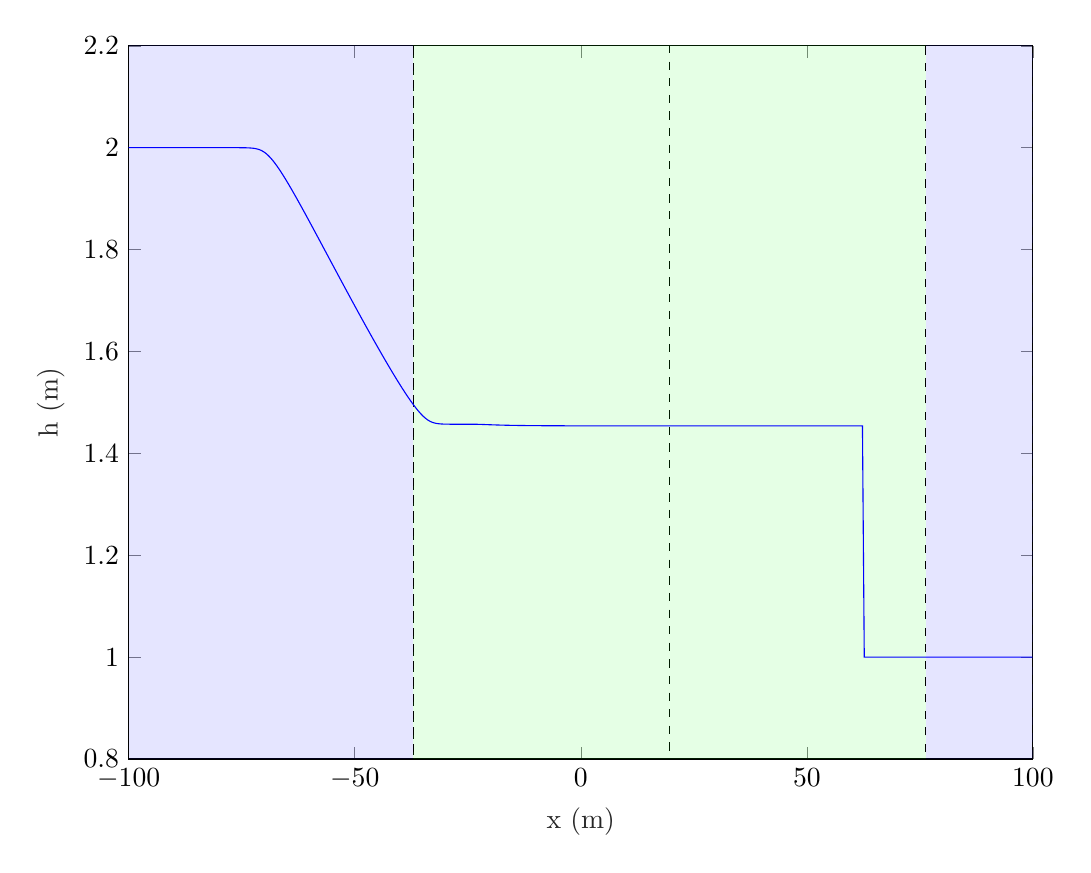
\begin{tikzpicture}

\begin{axis}[%
width=4.521in,
height=3.566in,
at={(0.758in,0.481in)},
scale only axis,
xmin=-100,
xmax=100,
xtick={-100,  -50,    0,   50,  100},
xlabel style={font=\color{white!15!black}},
xlabel={x (m)},
ymin=0.8,
ymax=2.2,
ytick={0.8,   1, 1.2, 1.4, 1.6, 1.8,   2, 2.2},
ylabel style={font=\color{white!15!black}},
ylabel={h (m)},
axis background/.style={fill=white}
]

\addplot[area legend, dashed, draw=black, fill=blue, fill opacity=0.1, forget plot]
table[row sep=crcr] {%
x	y\\
-100	-3\\
-100	3\\
-37.0630892039997	3\\
-37.0630892039997	-3\\
}--cycle;

\addplot[area legend, dashed, draw=black, fill=green, fill opacity=0.1, forget plot]
table[row sep=crcr] {%
x	y\\
-37.0630892039997	-3\\
-37.0630892039997	3\\
19.5890566189392	3\\
19.5890566189392	-3\\
}--cycle;

\addplot[area legend, draw=none, fill=green, fill opacity=0.1, forget plot]
table[row sep=crcr] {%
x	y\\
19.5890566189392	-3\\
19.5890566189392	3\\
76.2412024418781	3\\
76.2412024418781	-3\\
}--cycle;

\addplot[area legend, dashed, draw=black, fill=blue, fill opacity=0.1, forget plot]
table[row sep=crcr] {%
x	y\\
76.2412024418781	-3\\
76.2412024418781	3\\
100	3\\
100	-3\\
}--cycle;
\addplot [color=blue, forget plot]
  table[row sep=crcr]{%
-100.1200120012	2\\
-99.7199719971997	2\\
-99.3199319931993	2\\
-98.9198919891989	2\\
-98.5198519851985	2\\
-98.1198119811981	1.99999999999999\\
-97.7197719771977	1.99999999999999\\
-97.3197319731973	1.99999999999998\\
-96.9196919691969	1.99999999999997\\
-96.5196519651965	1.99999999999996\\
-96.1196119611961	1.99999999999994\\
-95.7195719571957	1.9999999999999\\
-95.3195319531953	1.99999999999985\\
-94.9194919491949	1.99999999999978\\
-94.5194519451945	1.99999999999968\\
-94.1194119411941	1.99999999999952\\
-93.7193719371937	1.99999999999928\\
-93.3193319331933	1.99999999999893\\
-92.9192919291929	1.99999999999841\\
-92.5192519251925	1.99999999999763\\
-92.1192119211921	1.99999999999645\\
-91.7191719171917	1.99999999999471\\
-91.3191319131913	1.99999999999211\\
-90.9190919091909	1.99999999998823\\
-90.5190519051905	1.99999999998244\\
-90.1190119011901	1.99999999997381\\
-89.7189718971897	1.99999999996092\\
-89.3189318931893	1.9999999999417\\
-88.9188918891889	1.99999999991303\\
-88.5188518851885	1.99999999987024\\
-88.1188118811881	1.99999999980642\\
-87.7187718771877	1.9999999997112\\
-87.3187318731873	1.99999999956914\\
-86.9186918691869	1.99999999935721\\
-86.5186518651865	1.99999999904103\\
-86.1186118611861	1.99999999856934\\
-85.7185718571857	1.99999999786562\\
-85.3185318531853	1.99999999681579\\
-84.9184918491849	1.99999999524965\\
-84.5184518451845	1.99999999291306\\
-84.1184118411841	1.99999998942711\\
-83.7183718371837	1.99999998422649\\
-83.3183318331833	1.99999997646775\\
-82.9182918291829	1.99999996489263\\
-82.5182518251825	1.99999994762391\\
-82.1182118211821	1.99999992186103\\
-81.7181718171817	1.99999988342592\\
-81.3181318131813	1.99999982608546\\
-80.9180918091809	1.99999974054077\\
-80.5180518051805	1.99999961291938\\
-80.1180118011801	1.99999942252614\\
-79.7179717971797	1.99999913848839\\
-79.3179317931793	1.99999871475237\\
-78.9178917891789	1.99999808262162\\
-78.5178517851785	1.99999713963222\\
-78.1178117811781	1.99999573297147\\
-77.7177717771777	1.9999936347754\\
-77.3177317731773	1.99999050535289\\
-76.9176917691769	1.99998583849213\\
-76.5176517651765	1.9999788802457\\
-76.1176117611761	1.99996850861262\\
-75.7175717571757	1.9999530559069\\
-75.3175317531753	1.9999300478715\\
-74.9174917491749	1.99989582350247\\
-74.5174517451745	1.99984498754921\\
-74.1174117411741	1.99976963611015\\
-73.7173717371737	1.99965829123995\\
-73.3173317331733	1.9994944977959\\
-72.9172917291729	1.99925510274861\\
-72.5172517251725	1.99890839587262\\
-72.1172117211721	1.99841257989026\\
-71.7171717171717	1.99771543194572\\
-71.3171317131713	1.99675631385204\\
-70.9170917091709	1.9954714453554\\
-70.5170517051705	1.99380215687772\\
-70.1170117011701	1.99170398312082\\
-69.7169716971697	1.98915330613979\\
-69.3169316931693	1.98614911632147\\
-68.9168916891689	1.98270988524878\\
-68.5168516851685	1.97886760275343\\
-68.1168116811681	1.97466143931244\\
-67.7167716771677	1.970132627673\\
-67.3167316731673	1.96532106420588\\
-66.9166916691669	1.96026343632199\\
-66.5166516651665	1.95499243781459\\
-66.1166116611661	1.94953665224664\\
-65.7165716571657	1.94392079435739\\
-65.3165316531653	1.93816611124749\\
-64.9164916491649	1.93229082911311\\
-64.5164516451645	1.92631058596417\\
-64.1164116411641	1.92023882323649\\
-63.7163716371637	1.91408712715289\\
-63.3163316331633	1.90786551988031\\
-62.9162916291629	1.90158270475123\\
-62.5162516251625	1.8952462713604\\
-62.1162116211621	1.88886286653179\\
-61.7161716171617	1.882438336706\\
-61.3161316131613	1.87597784661229\\
-60.9160916091609	1.86948597835872\\
-60.5160516051605	1.86296681438864\\
-60.1160116011601	1.85642400714998\\
-59.7159715971597	1.84986083781204\\
-59.3159315931593	1.84328026593763\\
-58.9158915891589	1.83668497166575\\
-58.5158515851585	1.83007739168943\\
-58.1158115811581	1.82345975010046\\
-57.7157715771577	1.81683408490893\\
-57.3157315731573	1.81020227075615\\
-56.9156915691569	1.80356603842666\\
-56.5156515651565	1.79692699228495\\
-56.1156115611561	1.79028662653726\\
-55.7155715571557	1.78364633952335\\
-55.3155315531553	1.77700744441394\\
-54.9154915491549	1.77037117724541\\
-54.5154515451545	1.76373870593444\\
-54.1154115411541	1.75711114130609\\
-53.7153715371537	1.75048954629397\\
-53.3153315331533	1.74387494115666\\
-52.9152915291529	1.73726830892092\\
-52.5152515251525	1.73067060420532\\
-52.1152115211521	1.724082760421\\
-51.7151715171517	1.71750569088851\\
-51.3151315131513	1.7109402903255\\
-50.9150915091509	1.70438744413148\\
-50.5150515051505	1.69784803921488\\
-50.1150115011501	1.69132296651589\\
-49.7149714971497	1.68481312018075\\
-49.3149314931493	1.67831940398103\\
-48.9148914891489	1.67184274159523\\
-48.5148514851485	1.66538408175274\\
-48.1148114811481	1.6589444012307\\
-47.7147714771477	1.65252471231067\\
-47.3147314731473	1.64612607190842\\
-46.9146914691469	1.63974958878497\\
-46.5146514651465	1.63339643165518\\
-46.1146114611461	1.62706783972849\\
-45.7145714571457	1.62076513407345\\
-45.3145314531453	1.61448973023413\\
-44.9144914491449	1.60824315305664\\
-44.5144514451445	1.60202705334846\\
-44.1144114411441	1.59584322702655\\
-43.7143714371437	1.58969363788087\\
-43.3143314331433	1.5835804442028\\
-42.9142914291429	1.57750602986162\\
-42.5142514251425	1.57147304074887\\
-42.1142114211421	1.56548442799472\\
-41.7141714171417	1.55954350043702\\
-41.3141314131413	1.55365398743191\\
-40.9140914091409	1.54782011308323\\
-40.5140514051405	1.54204668711773\\
-40.1140114011401	1.53633921627671\\
-39.7139713971397	1.53070403821826\\
-39.3139313931393	1.52514848596463\\
-38.9138913891389	1.51968108987095\\
-38.5138513851385	1.5143118230641\\
-38.1138113811381	1.50905240132486\\
-37.7137713771377	1.50391664422503\\
-37.3137313731373	1.49892090323306\\
-36.9136913691369	1.49408455351931\\
-36.5136513651365	1.48943052640473\\
-36.1136113611361	1.48498582243197\\
-35.7135713571357	1.48078187209598\\
-35.3135313531353	1.47685449630941\\
-34.9134913491349	1.47324304798179\\
-34.5134513451345	1.46998813572408\\
-34.1134113411341	1.46712730387127\\
-33.7133713371337	1.46468846189344\\
-33.3133313331333	1.46268207617707\\
-32.9132913291329	1.46109488711964\\
-32.5132513251325	1.45988875506157\\
-32.1132113211321	1.4590064235308\\
-31.7131713171317	1.45838208792976\\
-31.3131313131313	1.45795208117124\\
-30.9130913091309	1.45766194981287\\
-30.5130513051305	1.4574690933303\\
-30.1130113011301	1.45734222710925\\
-29.7129712971297	1.45725936162267\\
-29.3129312931293	1.45720549334089\\
-28.9128912891289	1.45717058633626\\
-28.5128512851285	1.4571480147833\\
-28.1128112811281	1.45713344150874\\
-27.7127712771277	1.45712404316205\\
-27.3127312731273	1.45711798826324\\
-26.9126912691269	1.4571140910178\\
-26.5126512651265	1.45711158362441\\
-26.1126112611261	1.45710996649685\\
-25.7125712571257	1.4571089075897\\
-25.3125312531253	1.45710816803852\\
-24.9124912491249	1.457107528681\\
-24.5124512451245	1.45710667099653\\
-24.1124112411241	1.45710486490965\\
-23.7123712371237	1.45710371215055\\
-23.3123312331233	1.45708072099705\\
-22.9122912291229	1.45699829445062\\
-22.5122512251225	1.45688959815283\\
-22.1122112211221	1.45677154074113\\
-21.7121712171217	1.45664491464926\\
-21.3121312131213	1.45651209686004\\
-20.9120912091209	1.4563762336698\\
-20.5120512051205	1.4562407158822\\
-20.1120112011201	1.4561076279883\\
-19.7119711971197	1.45597877122568\\
-19.3119311931193	1.45585564261276\\
-18.9118911891189	1.45573720326185\\
-18.5118511851185	1.45562469045578\\
-18.1118111811181	1.45551798493277\\
-17.7117711771177	1.45541740851169\\
-17.3117311731173	1.45532220343416\\
-16.9116911691169	1.45523238301776\\
-16.5116511651165	1.4551483705928\\
-16.1116111611161	1.45506884135665\\
-15.7115711571157	1.45499439414156\\
-15.3115311531153	1.45492438644256\\
-14.9114911491149	1.45485883434411\\
-14.5114511451145	1.45479722268867\\
-14.1114111411141	1.45473959405182\\
-13.7113711371137	1.45468562407338\\
-13.3113311331133	1.45463457952365\\
-12.9112911291129	1.45458704545768\\
-12.5112511251125	1.4545424604751\\
-12.1112111211121	1.45450062418416\\
-11.7111711171117	1.45446124443453\\
-11.3111311131113	1.45442448998106\\
-10.9110911091109	1.45438978910506\\
-10.5110511051105	1.45435757732522\\
-10.1110111011101	1.4543270349334\\
-9.71097109710971	1.45429860890565\\
-9.3109310931093	1.45427176571406\\
-8.9108910891089	1.45424662988252\\
-8.51085108510851	1.45422300079641\\
-8.11081108110811	1.45420080182472\\
-7.71077107710771	1.45417995087287\\
-7.31073107310731	1.45416037136018\\
-6.9106910691069	1.45414196043788\\
-6.5106510651065	1.45412466336458\\
-6.11061106110611	1.45410841177001\\
-5.71057105710571	1.45409317557675\\
-5.31053105310531	1.45407883047077\\
-4.91049104910491	1.45406519912513\\
-4.5104510451045	1.45405242271871\\
-4.1104110411041	1.4540405511109\\
-3.71037103710371	1.45402937138347\\
-3.31033103310331	1.4540184427968\\
-2.91029102910291	1.45400874627722\\
-2.51025102510251	1.45399937814984\\
-2.1102110211021	1.45399014353623\\
-1.7101710171017	1.45398214465648\\
-1.31013101310131	1.45397416262774\\
-0.91009100910091	1.45396670640899\\
-0.510051005100507	1.45395988386057\\
-0.110011001100105	1.45395296335125\\
0.290029002900297	1.4539471381016\\
0.6900690069007	1.45394089510847\\
1.09010901090109	1.45393577553495\\
1.49014901490149	1.45393018509531\\
1.89018901890189	1.45392563361382\\
2.2902290229023	1.45392060830841\\
2.6902690269027	1.45391662368743\\
3.0903090309031	1.45391204387055\\
3.4903490349035	1.45390856583632\\
3.89038903890389	1.45390452992925\\
4.29042904290429	1.45390131408687\\
4.6904690469047	1.45389785838778\\
5.0905090509051	1.45389469949931\\
5.4905490549055	1.45389211922005\\
5.8905890589059	1.45388906286769\\
6.29062906290629	1.45388671240873\\
6.69066906690669	1.45388404329426\\
7.0907090709071	1.45388180457463\\
7.4907490749075	1.45387956148363\\
7.8907890789079	1.45387716577817\\
8.2908290829083	1.45387552627158\\
8.69086908690869	1.45387340735488\\
9.09090909090909	1.45387182618569\\
9.4909490949095	1.45387034107157\\
9.8909890989099	1.45386857697808\\
10.2910291029103	1.45386715776617\\
10.6910691069107	1.45386580132301\\
11.0911091109111	1.45386411495782\\
11.4911491149115	1.45386315892391\\
11.8911891189119	1.45386219897224\\
12.2912291229123	1.45386095960166\\
12.6912691269127	1.45386011193179\\
13.0913091309131	1.45385907288651\\
13.4913491349135	1.45385781735207\\
13.8913891389139	1.45385709876387\\
14.2914291429143	1.45385643395316\\
14.6914691469147	1.45385553986828\\
15.0915091509151	1.45385486131625\\
15.4915491549155	1.45385405113379\\
15.8915891589159	1.4538531956454\\
16.2916291629163	1.45385270044113\\
16.6916691669167	1.45385218416127\\
17.0917091709171	1.45385153769841\\
17.4917491749175	1.45385083538883\\
17.8917891789179	1.45385043790226\\
18.2918291829183	1.45384988663998\\
18.6918691869187	1.45384948500253\\
19.0919091909191	1.453849085778\\
19.4919491949195	1.45384857833137\\
19.8919891989199	1.45384804398457\\
20.2920292029203	1.45384788344571\\
20.6920692069207	1.45384751022594\\
21.0921092109211	1.45384707426193\\
21.4921492149215	1.45384666912596\\
21.8921892189219	1.45384648688642\\
22.2922292229223	1.45384624617877\\
22.6922692269227	1.45384592999559\\
23.0923092309231	1.4538456928901\\
23.4923492349235	1.45384535373373\\
23.8923892389239	1.45384507554413\\
24.2924292429243	1.45384504069344\\
24.6924692469247	1.45384479425439\\
25.0925092509251	1.45384444870269\\
25.4925492549255	1.45384425976184\\
25.8925892589259	1.45384432041659\\
26.2926292629263	1.45384406814095\\
26.6926692669267	1.45384372856975\\
27.0927092709271	1.45384357438173\\
27.4927492749275	1.45384363797942\\
27.8927892789279	1.45384347709787\\
28.2928292829283	1.45384319715112\\
28.6928692869287	1.4538430620842\\
29.0929092909291	1.45384310510292\\
29.4929492949295	1.45384296346383\\
29.8929892989299	1.45384280192386\\
30.2930293029303	1.45384271484652\\
30.6930693069307	1.45384260646391\\
31.0931093109311	1.45384260850224\\
31.4931493149315	1.45384254734809\\
31.8931893189319	1.4538423159154\\
32.2932293229323	1.45384214620777\\
32.6932693269327	1.45384232004519\\
33.0933093309331	1.45384229706708\\
33.4933493349335	1.45384199601712\\
33.8933893389339	1.45384185997374\\
34.2934293429343	1.4538421306342\\
34.6934693469347	1.45384211382159\\
35.0935093509351	1.45384173623127\\
35.4935493549355	1.45384162846269\\
35.8935893589359	1.45384191934021\\
36.2936293629363	1.45384189611905\\
36.6936693669367	1.45384154110284\\
37.0937093709371	1.45384146287123\\
37.4937493749375	1.45384173531721\\
37.8937893789379	1.45384172720275\\
38.2938293829383	1.45384141243441\\
38.6938693869387	1.45384134099888\\
39.0939093909391	1.45384158479125\\
39.4939493949395	1.45384155797275\\
39.8939893989399	1.45384133245515\\
40.2940294029403	1.45384128883434\\
40.6940694069407	1.45384142267247\\
41.0941094109411	1.45384139594244\\
41.4941494149415	1.45384132562301\\
41.8941894189419	1.45384125209301\\
42.2942294229423	1.45384122301705\\
42.6942694269427	1.45384134345942\\
43.0943094309431	1.45384140577262\\
43.4943494349435	1.4538410934293\\
43.8943894389439	1.45384102191432\\
44.2944294429443	1.45384132220724\\
44.6944694469447	1.45384143353312\\
45.0945094509451	1.45384096141764\\
45.4945494549455	1.45384092192721\\
45.8945894589459	1.45384132111373\\
46.2946294629463	1.45384144054848\\
46.6946694669467	1.45384086150238\\
47.0947094709471	1.45384086453025\\
47.4947494749475	1.45384138393006\\
47.8947894789479	1.45384138878154\\
48.2948294829483	1.45384078591114\\
48.6948694869487	1.4538408062737\\
49.0949094909491	1.45384142023876\\
49.4949494949495	1.45384125091577\\
49.8949894989499	1.45384077977479\\
50.2950295029503	1.4538407033293\\
50.6950695069507	1.45384149762261\\
51.0951095109511	1.45384103754554\\
51.4951495149515	1.4538409031074\\
51.8951895189519	1.45384046245381\\
52.2952295229523	1.45384174887457\\
52.6952695269527	1.45384066621454\\
53.0953095309531	1.45384130750493\\
53.4953495349535	1.4538399846453\\
53.8953895389539	1.45384225595284\\
54.2954295429543	1.45383988248501\\
54.6954695469547	1.45384227628999\\
55.0955095509551	1.45383890753286\\
55.4955495549555	1.4538434023746\\
55.8955895589559	1.45383837477877\\
56.2956295629563	1.45384433081865\\
56.6956695669567	1.45383656783735\\
57.0957095709571	1.45384562775157\\
57.4957495749575	1.45383547088346\\
57.8957895789579	1.45384841769518\\
58.2958295829583	1.45383179515641\\
58.6958695869587	1.45385061405405\\
59.0959095909591	1.45382925917418\\
59.4959495949595	1.45385607967265\\
59.8959895989599	1.45382262123379\\
60.2960296029603	1.45386066778075\\
60.6960696069607	1.45381704652221\\
61.0961096109611	1.45386966597628\\
61.4961496149615	1.4538061088152\\
61.8961896189619	1.45387662285077\\
62.2962296229623	1.45379093546777\\
62.6962696269627	1.00012576995479\\
63.0963096309631	1.00000005035169\\
63.4963496349635	1.00000003375035\\
63.8963896389639	1.00000002262261\\
64.2964296429643	1.00000001516377\\
64.6964696469647	1.00000001016418\\
65.0965096509651	1.00000000681298\\
65.4965496549655	1.00000000456669\\
65.8965896589659	1.00000000306101\\
66.2966296629663	1.00000000205179\\
66.6966696669667	1.00000000137529\\
67.0967096709671	1.00000000092187\\
67.4967496749675	1.00000000061791\\
67.8967896789679	1.00000000041416\\
68.2968296829683	1.00000000027761\\
68.6968696869687	1.00000000018608\\
69.0969096909691	1.00000000012473\\
69.4969496949695	1.00000000008361\\
69.8969896989699	1.00000000005605\\
70.2970297029703	1.00000000003758\\
70.6970697069707	1.0000000000252\\
71.0971097109711	1.0000000000169\\
71.4971497149715	1.0000000000113\\
71.8971897189719	1.00000000000762\\
72.2972297229723	1.00000000000511\\
72.6972697269727	1.00000000000336\\
73.0973097309731	1.00000000000224\\
73.4973497349735	1.00000000000151\\
73.8973897389739	1.00000000000101\\
74.2974297429743	1.0000000000007\\
74.6974697469747	1.00000000000048\\
75.0975097509751	1.00000000000036\\
75.4975497549755	1.00000000000023\\
75.8975897589759	1.00000000000017\\
76.2976297629763	1.00000000000013\\
76.6976697669767	1.00000000000007\\
77.0977097709771	1.00000000000002\\
77.4977497749775	1\\
77.8977897789779	1\\
78.2978297829783	1\\
78.6978697869787	1\\
79.0979097909791	1\\
79.4979497949795	1\\
79.8979897989799	1\\
80.2980298029803	1\\
80.6980698069807	1\\
81.0981098109811	1\\
81.4981498149815	1\\
81.8981898189819	1\\
82.2982298229823	1\\
82.6982698269827	1\\
83.0983098309831	1\\
83.4983498349835	1\\
83.8983898389839	1\\
84.2984298429843	1\\
84.6984698469847	1\\
85.0985098509851	1\\
85.4985498549855	1\\
85.8985898589859	1\\
86.2986298629863	1\\
86.6986698669867	1\\
87.0987098709871	1\\
87.4987498749875	1\\
87.8987898789879	1\\
88.2988298829883	1\\
88.6988698869887	1\\
89.0989098909891	1\\
89.4989498949895	1\\
89.8989898989899	1\\
90.2990299029903	1\\
90.6990699069907	1\\
91.0991099109911	1\\
91.4991499149915	1\\
91.8991899189919	1\\
92.2992299229923	1\\
92.6992699269927	1\\
93.0993099309931	1\\
93.4993499349935	1\\
93.8993899389939	1\\
94.2994299429943	1\\
94.6994699469947	1\\
95.0995099509951	1\\
95.4995499549955	1\\
95.8995899589959	1\\
96.2996299629963	1\\
96.6996699669967	1\\
97.0997099709971	1\\
97.4997499749975	1\\
97.8997899789979	1\\
98.2998299829983	1\\
98.6998699869987	1\\
99.0999099909991	1\\
99.4999499949995	1\\
99.8999899989999	1\\
};
\end{axis}
\end{tikzpicture}%
		\caption{$h$}
	\end{subfigure}
	\begin{subfigure}{0.49\textwidth}
		\centering
		% This file was created by matlab2tikz.
%
%The latest updates can be retrieved from
%  http://www.mathworks.com/matlabcentral/fileexchange/22022-matlab2tikz-matlab2tikz
%where you can also make suggestions and rate matlab2tikz.
%
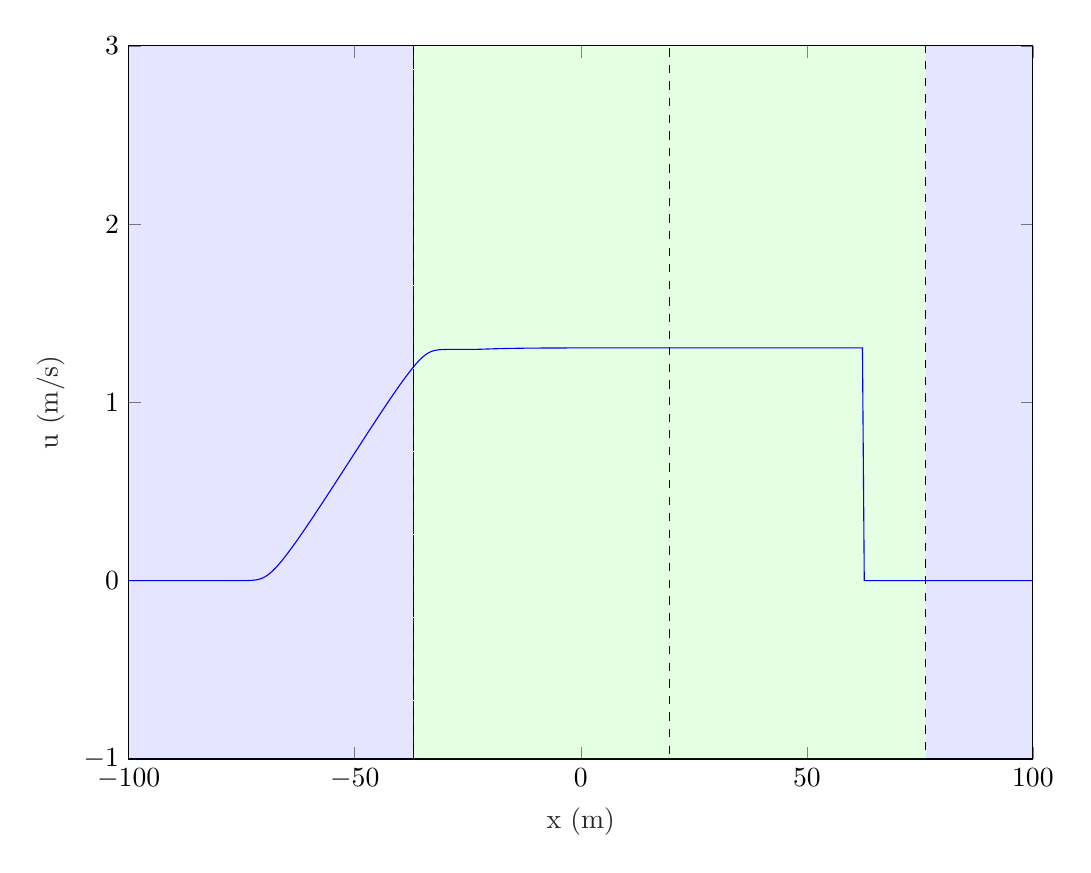
\begin{tikzpicture}

\begin{axis}[%
width=4.521in,
height=3.566in,
at={(0.758in,0.481in)},
scale only axis,
xmin=-100,
xmax=100,
xtick={-100,  -50,    0,   50,  100},
xlabel style={font=\color{white!15!black}},
xlabel={x (m)},
ymin=-1,
ymax=3,
ytick={-1,  0,  1,  2,  3},
ylabel style={font=\color{white!15!black}},
ylabel={u (m/s)},
axis background/.style={fill=white}
]

\addplot[area legend, dashed, draw=black, fill=blue, fill opacity=0.1, forget plot]
table[row sep=crcr] {%
x	y\\
-100	-3\\
-100	3\\
-37.0630892039997	3\\
-37.0630892039997	-3\\
}--cycle;

\addplot[area legend, dashed, draw=black, fill=green, fill opacity=0.1, forget plot]
table[row sep=crcr] {%
x	y\\
-37.0630892039997	-3\\
-37.0630892039997	3\\
19.5890566189392	3\\
19.5890566189392	-3\\
}--cycle;

\addplot[area legend, draw=none, fill=green, fill opacity=0.1, forget plot]
table[row sep=crcr] {%
x	y\\
19.5890566189392	-3\\
19.5890566189392	3\\
76.2412024418781	3\\
76.2412024418781	-3\\
}--cycle;

\addplot[area legend, dashed, draw=black, fill=blue, fill opacity=0.1, forget plot]
table[row sep=crcr] {%
x	y\\
76.2412024418781	-3\\
76.2412024418781	3\\
100	3\\
100	-3\\
}--cycle;
\addplot [color=blue, forget plot]
  table[row sep=crcr]{%
-100.1200120012	0\\
-99.7199719971997	1.20310066172386e-15\\
-99.3199319931993	1.20310066172386e-15\\
-98.9198919891989	1.20310066172386e-15\\
-98.5198519851985	4.01033553907953e-15\\
-98.1198119811981	1.26325569481006e-14\\
-97.7197719771977	2.13550367455986e-14\\
-97.3197319731973	3.85994795636408e-14\\
-96.9196919691969	6.17591673018257e-14\\
-96.5196519651965	9.74511535996348e-14\\
-96.1196119611961	1.35749857997846e-13\\
-95.7195719571957	2.18362770102891e-13\\
-95.3195319531953	3.22631494118972e-13\\
-94.9194919491949	4.79034580143102e-13\\
-94.5194519451945	7.1424075951018e-13\\
-94.1194119411941	1.06434305207196e-12\\
-93.7193719371937	1.58558641376414e-12\\
-93.3193319331933	2.35988194797261e-12\\
-92.9192919291929	3.51886891876813e-12\\
-92.5192519251925	5.25975557628601e-12\\
-92.1192119211921	7.8533398278049e-12\\
-91.7191719171917	1.17064702137695e-11\\
-91.3191319131913	1.74745358196656e-11\\
-90.9190919091909	2.60646745444584e-11\\
-90.5190519051905	3.88802030517174e-11\\
-90.1190119011901	5.80086012480489e-11\\
-89.7189718971897	8.6539030599488e-11\\
-89.3189318931893	1.29104732013351e-10\\
-88.9188918891889	1.92611703806107e-10\\
-88.5188518851885	2.87357384802956e-10\\
-88.1188118811881	4.28703866585211e-10\\
-87.7187718771877	6.39581245196873e-10\\
-87.3187318731873	9.54182644062348e-10\\
-86.9186918691869	1.42352805327816e-09\\
-86.5186518651865	2.12373674955616e-09\\
-86.1186118611861	3.16836589569138e-09\\
-85.7185718571857	4.72682680368017e-09\\
-85.3185318531853	7.05179607999013e-09\\
-84.9184918491849	1.05201874203771e-08\\
-84.5184518451845	1.56948281670943e-08\\
-84.1184118411841	2.34148462627066e-08\\
-83.7183718371837	3.49322089550453e-08\\
-83.3183318331833	5.21148211584671e-08\\
-82.9182918291829	7.77492299605816e-08\\
-82.5182518251825	1.15992747197557e-07\\
-82.1182118211821	1.73047553814648e-07\\
-81.7181718171817	2.581664368374e-07\\
-81.3181318131813	3.85153335609719e-07\\
-80.9180918091809	5.74601711342825e-07\\
-80.5180518051805	8.57233696637947e-07\\
-80.1180118011801	1.27888103023171e-06\\
-79.7179717971797	1.90791476353846e-06\\
-79.3179317931793	2.84632620362215e-06\\
-78.9178917891789	4.24625156482475e-06\\
-78.5178517851785	6.33460918633692e-06\\
-78.1178117811781	9.44982089550209e-06\\
-77.7177717771777	1.40965190991419e-05\\
-77.3177317731773	2.10269925014753e-05\\
-76.9176917691769	3.13623140245558e-05\\
-76.5176517651765	4.67722070155116e-05\\
-76.1176117611761	6.9741517600241e-05\\
-75.7175717571757	0.000103963631895029\\
-75.3175317531753	0.000154918309112971\\
-74.9174917491749	0.000230713781119599\\
-74.5174517451745	0.000343299596139778\\
-74.1174117411741	0.000510182368859854\\
-73.7173717371737	0.000756786804900984\\
-73.3173317331733	0.00111956648080909\\
-72.9172917291729	0.00164982131205373\\
-72.5172517251725	0.00241782853176445\\
-72.1172117211721	0.00351625535406051\\
-71.7171717171717	0.00506095058718152\\
-71.3171317131713	0.00718655629407767\\
-70.9170917091709	0.0100349115555877\\
-70.5170517051705	0.0137368587699572\\
-70.1170117011701	0.0183921576435123\\
-69.7169716971697	0.024054765915593\\
-69.3169316931693	0.0307288634802072\\
-68.9168916891689	0.0383756546573989\\
-68.5168516851685	0.0469264410789162\\
-68.1168116811681	0.0562965466373097\\
-67.7167716771677	0.0663965792756074\\
-67.3167316731673	0.0771399202324\\
-66.9166916691669	0.0884468608222327\\
-66.5166516651665	0.100246346979299\\
-66.1166116611661	0.112476253321195\\
-65.7165716571657	0.125082867878753\\
-65.3165316531653	0.138020023322745\\
-64.9164916491649	0.151248126011885\\
-64.5164516451645	0.16473321407373\\
-64.1164116411641	0.178446104339091\\
-63.7163716371637	0.192361648476996\\
-63.3163316331633	0.206458098437861\\
-62.9162916291629	0.220716572000128\\
-62.5162516251625	0.235120605794511\\
-62.1162116211621	0.249655782749358\\
-61.7161716171617	0.264309421856854\\
-61.3161316131613	0.279070319649349\\
-60.9160916091609	0.293928534366848\\
-60.5160516051605	0.308875205290471\\
-60.1160116011601	0.323902401030126\\
-59.7159715971597	0.339002991670815\\
-59.3159315931593	0.354170540614654\\
-58.9158915891589	0.369399212725129\\
-58.5158515851585	0.384683695969387\\
-58.1158115811581	0.400019134215722\\
-57.7157715771577	0.415401069428963\\
-57.3157315731573	0.430825392159617\\
-56.9156915691569	0.446288299007442\\
-56.5156515651565	0.461786254507809\\
-56.1156115611561	0.477315955380278\\
-55.7155715571557	0.492874299028364\\
-55.3155315531553	0.508458360159185\\
-54.9154915491549	0.52406537343213\\
-54.5154515451545	0.539692713616919\\
-54.1154115411541	0.5553378707805\\
-53.7153715371537	0.570998429534588\\
-53.3153315331533	0.586672057512476\\
-52.9152915291529	0.602356493184321\\
-52.5152515251525	0.618049525486038\\
-52.1152115211521	0.633748977093646\\
-51.7151715171517	0.649452702062043\\
-51.3151315131513	0.66515858255626\\
-50.9150915091509	0.680864506832353\\
-50.5150515051505	0.696568343258946\\
-50.1150115011501	0.712267934056549\\
-49.7149714971497	0.72796109705572\\
-49.3149314931493	0.743645609952727\\
-48.9148914891489	0.759319185027259\\
-48.5148514851485	0.774979456054229\\
-48.1148114811481	0.790623970295332\\
-47.7147714771477	0.80625016953149\\
-47.3147314731473	0.821855366799539\\
-46.9146914691469	0.837436727569459\\
-46.5146514651465	0.852991248515498\\
-46.1146114611461	0.868515730081942\\
-45.7145714571457	0.884006746725078\\
-45.3145314531453	0.899460613748151\\
-44.9144914491449	0.91487334831991\\
-44.5144514451445	0.930240625542571\\
-44.1144114411441	0.945557727884106\\
-43.7143714371437	0.960819485097442\\
-43.3143314331433	0.976020203893531\\
-42.9142914291429	0.991153585795962\\
-42.5142514251425	1.00621263074525\\
-42.1142114211421	1.02118952278069\\
-41.7141714171417	1.03607549137923\\
-41.3141314131413	1.05086064544801\\
-40.9140914091409	1.0655337769765\\
-40.5140514051405	1.08008212085858\\
-40.1140114011401	1.09449106066237\\
-39.7139713971397	1.10874377478788\\
-39.3139313931393	1.12282080210799\\
-38.9138913891389	1.13669950868161\\
-38.5138513851385	1.1503534396329\\
-38.1138113811381	1.16375152743987\\
-37.7137713771377	1.17685713841157\\
-37.3137313731373	1.18962694208758\\
-36.9136913691369	1.20200961167313\\
-36.5136513651365	1.21394441526928\\
-36.1136113611361	1.22535985435855\\
-35.7135713571357	1.23617269670773\\
-35.3135313531353	1.24628805191909\\
-34.9134913491349	1.2556015850068\\
-34.5134513451345	1.26400543698337\\
-34.1134113411341	1.27139949563096\\
-33.7133713371337	1.2777085700091\\
-33.3133313331333	1.28290283848493\\
-32.9132913291329	1.2870143633742\\
-32.5132513251325	1.29014025134544\\
-32.1132113211321	1.29242775556672\\
-31.7131713171317	1.29404679181074\\
-31.3131313131313	1.2951620846585\\
-30.9130913091309	1.29591467604957\\
-30.5130513051305	1.29641497865511\\
-30.1130113011301	1.29674410821519\\
-29.7129712971297	1.29695909372152\\
-29.3129312931293	1.2970988521828\\
-28.9128912891289	1.29718941787276\\
-28.5128512851285	1.29724797995161\\
-28.1128112811281	1.29728579064746\\
-27.7127712771277	1.29731017495848\\
-27.3127312731273	1.29732588461647\\
-26.9126912691269	1.29733599616931\\
-26.5126512651265	1.29734250169265\\
-26.1126112611261	1.29734669737661\\
-25.7125712571257	1.29734944471939\\
-25.3125312531253	1.29735136344624\\
-24.9124912491249	1.29735302212976\\
-24.5124512451245	1.2973552470104\\
-24.1124112411241	1.29735993399805\\
-23.7123712371237	1.29736291431688\\
-23.3123312331233	1.2974225197586\\
-22.9122912291229	1.29763643330677\\
-22.5122512251225	1.2979185006304\\
-22.1122112211221	1.29822485669061\\
-21.7121712171217	1.29855346176069\\
-21.3121312131213	1.29889815015816\\
-20.9120912091209	1.29925075844605\\
-20.5120512051205	1.29960248573119\\
-20.1120112011201	1.29994792269806\\
-19.7119711971197	1.3002823913133\\
-19.3119311931193	1.30060200162737\\
-18.9118911891189	1.30090945888353\\
-18.5118511851185	1.30120153985293\\
-18.1118111811181	1.30147855656157\\
-17.7117711771177	1.30173966836207\\
-17.3117311731173	1.3019868468062\\
-16.9116911691169	1.30222005050906\\
-16.5116511651165	1.30243817879373\\
-16.1116111611161	1.30264467913955\\
-15.7115711571157	1.30283798491811\\
-15.3115311531153	1.30301976949735\\
-14.9114911491149	1.30318998685069\\
-14.5114511451145	1.30334997610034\\
-14.1114111411141	1.30349962230142\\
-13.7113711371137	1.30363977242428\\
-13.3113311331133	1.30377233343227\\
-12.9112911291129	1.30389577505745\\
-12.5112511251125	1.30401156009271\\
-12.1112111211121	1.30412020885993\\
-11.7111711171117	1.30422248158839\\
-11.3111311131113	1.30431793652427\\
-10.9110911091109	1.30440805985393\\
-10.5110511051105	1.30449171650979\\
-10.1110111011101	1.30457104071167\\
-9.71097109710971	1.30464486789461\\
-9.3109310931093	1.30471458671827\\
-8.9108910891089	1.30477987036077\\
-8.51085108510851	1.30484124131316\\
-8.11081108110811	1.30489889841681\\
-7.71077107710771	1.30495305471611\\
-7.31073107310731	1.30500390903438\\
-6.9106910691069	1.30505172834054\\
-6.5106510651065	1.30509665526714\\
-6.11061106110611	1.30513886680985\\
-5.71057105710571	1.30517844085529\\
-5.31053105310531	1.30521570099188\\
-4.91049104910491	1.3052511069201\\
-4.5104510451045	1.3052842932094\\
-4.1104110411041	1.30531512896904\\
-3.71037103710371	1.3053441662328\\
-3.31033103310331	1.3053725551244\\
-2.91029102910291	1.30539773921867\\
-2.51025102510251	1.30542207216032\\
-2.1102110211021	1.30544606164796\\
-1.7101710171017	1.30546683651675\\
-1.31013101310131	1.30548756981708\\
-0.91009100910091	1.30550693748858\\
-0.510051005100507	1.30552465810747\\
-0.110011001100105	1.30554263686578\\
0.290029002900297	1.30555776523837\\
0.6900690069007	1.30557398476534\\
1.09010901090109	1.30558728008809\\
1.49014901490149	1.30560180427017\\
1.89018901890189	1.30561362430008\\
2.2902290229023	1.30562668107364\\
2.6902690269027	1.30563702806527\\
3.0903090309031	1.30564892817702\\
3.4903490349035	1.30565795880588\\
3.89038903890389	1.30566844505804\\
4.29042904290429	1.3056767959318\\
4.6904690469047	1.30568577345668\\
5.0905090509051	1.30569397816428\\
5.4905490549055	1.3057006770733\\
5.8905890589059	1.30570861919236\\
6.29062906290629	1.30571472107098\\
6.69066906690669	1.30572165738072\\
7.0907090709071	1.30572747228334\\
7.4907490749075	1.30573329942128\\
7.8907890789079	1.30573952637631\\
8.2908290829083	1.30574378169663\\
8.69086908690869	1.30574928820404\\
9.09090909090909	1.30575339229335\\
9.4909490949095	1.30575724618737\\
9.8909890989099	1.30576183190729\\
10.2910291029103	1.30576551797092\\
10.6910691069107	1.30576904164719\\
11.0911091109111	1.30577342908797\\
11.4911491149115	1.30577590673361\\
11.8911891189119	1.30577839787863\\
12.2912291229123	1.30578161824587\\
12.6912691269127	1.30578381760958\\
13.0913091309131	1.30578651899322\\
13.4913491349135	1.30578978356086\\
13.8913891389139	1.30579164794159\\
14.2914291429143	1.30579337301564\\
14.6914691469147	1.30579569597634\\
15.0915091509151	1.30579745752971\\
15.4915491549155	1.30579956371143\\
15.8915891589159	1.30580178795792\\
16.2916291629163	1.30580307093907\\
16.6916691669167	1.30580441122207\\
17.0917091709171	1.30580609196488\\
17.4917491749175	1.30580791791099\\
17.8917891789179	1.30580894965695\\
18.2918291829183	1.30581038180852\\
18.6918691869187	1.30581142243842\\
19.0919091909191	1.30581246031084\\
19.4919491949195	1.30581377946989\\
19.8919891989199	1.30581516987843\\
20.2920292029203	1.30581558074711\\
20.6920692069207	1.30581655289925\\
21.0921092109211	1.30581768590077\\
21.4921492149215	1.30581873907574\\
21.8921892189219	1.30581921028597\\
22.2922292229223	1.30581983569932\\
22.6922692269227	1.30582065772077\\
23.0923092309231	1.30582127373313\\
23.4923492349235	1.30582215476747\\
23.8923892389239	1.30582288151672\\
24.2924292429243	1.30582296523233\\
24.6924692469247	1.30582360540208\\
25.0925092509251	1.30582450622945\\
25.4925492549255	1.30582500260415\\
25.8925892589259	1.30582483573873\\
26.2926292629263	1.30582548984399\\
26.6926692669267	1.30582637634858\\
27.0927092709271	1.3058267825951\\
27.4927492749275	1.30582660777596\\
27.8927892789279	1.30582702648096\\
28.2928292829283	1.30582775672676\\
28.6928692869287	1.30582811001879\\
29.0929092909291	1.30582799207957\\
29.4929492949295	1.30582836192636\\
29.8929892989299	1.30582878197032\\
30.2930293029303	1.30582900779783\\
30.6930693069307	1.30582929148594\\
31.0931093109311	1.30582928069418\\
31.4931493149315	1.3058294416002\\
31.8931893189319	1.30583004602972\\
32.2932293229323	1.30583048534975\\
32.6932693269327	1.30583002764876\\
33.0933093309331	1.30583009035634\\
33.4933493349335	1.30583087756881\\
33.8933893389339	1.3058312291948\\
34.2934293429343	1.30583051814444\\
34.6934693469347	1.30583056432427\\
35.0935093509351	1.30583155210788\\
35.4935493549355	1.30583183070653\\
35.8935893589359	1.30583106618729\\
36.2936293629363	1.30583112855916\\
36.6936693669367	1.30583205817193\\
37.0937093709371	1.30583225899129\\
37.4937493749375	1.30583154387666\\
37.8937893789379	1.30583156734215\\
38.2938293829383	1.30583239158334\\
38.6938693869387	1.30583257471396\\
39.0939093909391	1.30583193506839\\
39.4939493949395	1.30583200687202\\
39.8939893989399	1.30583259704103\\
40.2940294029403	1.30583270865001\\
40.6940694069407	1.30583235733094\\
41.0941094109411	1.30583242850931\\
41.4941494149415	1.30583261026248\\
41.8941894189419	1.30583280236354\\
42.2942294229423	1.30583287847741\\
42.6942694269427	1.30583256115841\\
43.0943094309431	1.30583239865085\\
43.4943494349435	1.30583321686745\\
43.8943894389439	1.30583339996667\\
44.2944294429443	1.30583261284275\\
44.6944694469447	1.3058323219765\\
45.0945094509451	1.30583355919421\\
45.4945494549455	1.30583365930063\\
45.8945894589459	1.30583261079062\\
46.2946294629463	1.30583229206305\\
46.6946694669467	1.30583381695887\\
47.0947094709471	1.3058338063623\\
47.4947494749475	1.30583244106974\\
47.8947894789479	1.30583242595369\\
48.2948294829483	1.30583400982424\\
48.6948694869487	1.30583395415898\\
49.0949094909491	1.30583233432749\\
49.4949494949495	1.3058328023817\\
49.8949894989499	1.30583402441377\\
50.2950295029503	1.30583422829934\\
50.6950695069507	1.30583212098331\\
51.0951095109511	1.3058333794263\\
51.4951495149515	1.30583367507895\\
51.8951895189519	1.30583487379059\\
52.2952295229523	1.30583143723593\\
52.6952695269527	1.3058343745553\\
53.0953095309531	1.30583258310065\\
53.4953495349535	1.30583612439725\\
53.8953895389539	1.30583008303063\\
54.2954295429543	1.30583642746269\\
54.6954695469547	1.3058300536614\\
55.0955095509551	1.3058389415638\\
55.4955495549555	1.30582708789906\\
55.8955895589559	1.30584035074381\\
56.2956295629563	1.30582460395265\\
56.6956695669567	1.30584508291233\\
57.0957095709571	1.30582115280522\\
57.4957495749575	1.30584783370659\\
57.8957895789579	1.30581397604087\\
58.2958295829583	1.30585722342469\\
58.6958695869587	1.30580821688969\\
59.0959095909591	1.30586358369973\\
59.4959495949595	1.3057936967549\\
59.8959895989599	1.3058807033107\\
60.2960296029603	1.30578093808863\\
60.6960696069607	1.30589543610573\\
61.0961096109611	1.3057554739883\\
61.4961496149615	1.30592420376048\\
61.8961896189619	1.30573544324779\\
62.2962296229623	1.30596833368334\\
62.6962696269627	0.000332225261428372\\
63.0963096309631	1.57698244619973e-07\\
63.4963496349635	1.05703905494044e-07\\
63.8963896389639	7.08525549637964e-08\\
64.2964296429643	4.74919504983337e-08\\
64.6964696469647	3.1833543146939e-08\\
65.0965096509651	2.13378173222618e-08\\
65.4965496549655	1.43025674767e-08\\
65.8965896589659	9.58689791866647e-09\\
66.2966296629663	6.42606605826271e-09\\
66.6966696669667	4.3073205304687e-09\\
67.0967096709671	2.8872363064252e-09\\
67.4967496749675	1.93524165297519e-09\\
67.8967896789679	1.2971278404322e-09\\
68.2968296829683	8.69453276929635e-10\\
68.6968696869687	5.82798703581465e-10\\
69.0969096909691	3.90647737267702e-10\\
69.4969496949695	2.61858618691872e-10\\
69.8969896989699	1.75541209273858e-10\\
70.2970297029703	1.17701643674957e-10\\
70.6970697069707	7.89289677476568e-11\\
71.0971097109711	5.29457030158889e-11\\
71.4971497149715	3.53905093232577e-11\\
71.8971897189719	2.38565336671119e-11\\
72.2972297229723	1.60123674819664e-11\\
72.6972697269727	1.0519260506553e-11\\
73.0973097309731	7.01538021688458e-12\\
73.4973497349735	4.71535252684261e-12\\
73.8973897389739	3.16214957256102e-12\\
74.2974297429743	2.1952576740906e-12\\
74.6974697469747	1.5110443019302e-12\\
75.0975097509751	1.1329699189838e-12\\
75.4975497549755	7.3604695900364e-13\\
75.8975897589759	5.54880051025796e-13\\
76.2976297629763	4.02888334094727e-13\\
76.6976697669767	2.35757600503621e-13\\
77.0977097709771	6.8927642077928e-14\\
77.4977497749775	0\\
77.8977897789779	0\\
78.2978297829783	0\\
78.6978697869787	0\\
79.0979097909791	0\\
79.4979497949795	0\\
79.8979897989799	0\\
80.2980298029803	0\\
80.6980698069807	0\\
81.0981098109811	0\\
81.4981498149815	0\\
81.8981898189819	0\\
82.2982298229823	0\\
82.6982698269827	0\\
83.0983098309831	0\\
83.4983498349835	0\\
83.8983898389839	0\\
84.2984298429843	0\\
84.6984698469847	0\\
85.0985098509851	0\\
85.4985498549855	0\\
85.8985898589859	0\\
86.2986298629863	0\\
86.6986698669867	0\\
87.0987098709871	0\\
87.4987498749875	0\\
87.8987898789879	0\\
88.2988298829883	0\\
88.6988698869887	0\\
89.0989098909891	0\\
89.4989498949895	0\\
89.8989898989899	0\\
90.2990299029903	0\\
90.6990699069907	0\\
91.0991099109911	0\\
91.4991499149915	0\\
91.8991899189919	0\\
92.2992299229923	0\\
92.6992699269927	0\\
93.0993099309931	0\\
93.4993499349935	0\\
93.8993899389939	0\\
94.2994299429943	0\\
94.6994699469947	0\\
95.0995099509951	0\\
95.4995499549955	0\\
95.8995899589959	0\\
96.2996299629963	0\\
96.6996699669967	0\\
97.0997099709971	0\\
97.4997499749975	0\\
97.8997899789979	0\\
98.2998299829983	0\\
98.6998699869987	0\\
99.0999099909991	0\\
99.4999499949995	0\\
99.8999899989999	0\\
};
\end{axis}
\end{tikzpicture}%
		\caption{$u$}
	\end{subfigure}
	\caption{Solution of gSGN with $\beta_1 = -\dfrac{2}{3} $ and $\beta_2 = 0$ (Shallow Water Wave Equations) for smooth dam-break problem at $t=15s$ with inequality regions shown.}
	\label{fig:SWWESDB}
\end{figure}

\begin{figure}
	\tikzset{every picture/.style={scale=0.75}}%
	\centering
	\begin{subfigure}{0.49\textwidth}
		\centering
		% This file was created by matlab2tikz.
%
%The latest updates can be retrieved from
%  http://www.mathworks.com/matlabcentral/fileexchange/22022-matlab2tikz-matlab2tikz
%where you can also make suggestions and rate matlab2tikz.
%
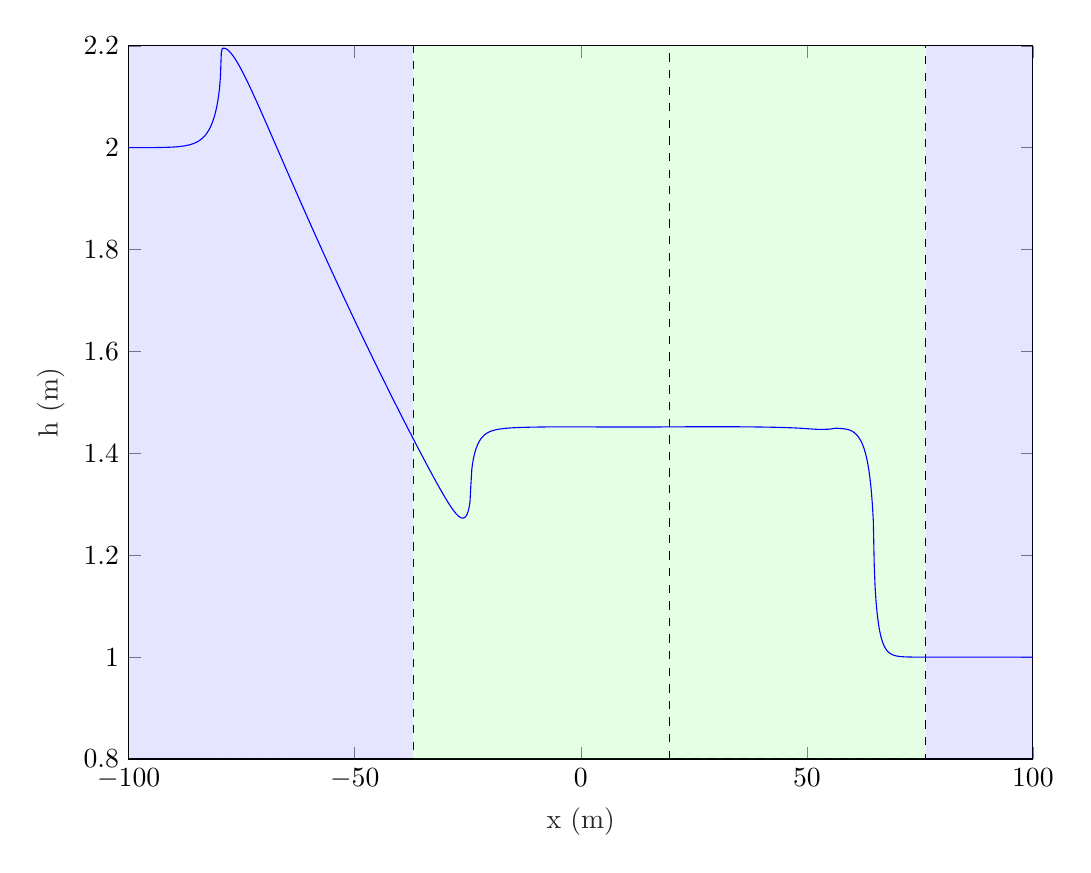
\begin{tikzpicture}

\begin{axis}[%
width=4.521in,
height=3.566in,
at={(0.758in,0.481in)},
scale only axis,
xmin=-100,
xmax=100,
xtick={-100,  -50,    0,   50,  100},
xlabel style={font=\color{white!15!black}},
xlabel={x (m)},
ymin=0.8,
ymax=2.2,
ytick={0.8,   1, 1.2, 1.4, 1.6, 1.8,   2, 2.2},
ylabel style={font=\color{white!15!black}},
ylabel={h (m)},
axis background/.style={fill=white}
]

\addplot[area legend, dashed, draw=black, fill=blue, fill opacity=0.1, forget plot]
table[row sep=crcr] {%
x	y\\
-100	0.8\\
-100	2.2\\
-37.0630892039997	2.2\\
-37.0630892039997	0.8\\
}--cycle;

\addplot[area legend, draw=none, fill=green, fill opacity=0.1, forget plot]
table[row sep=crcr] {%
x	y\\
-37.0630892039997	0.8\\
-37.0630892039997	2.2\\
19.5890566189392	2.2\\
19.5890566189392	0.8\\
}--cycle;

\addplot[area legend, dashed, draw=black, fill=green, fill opacity=0.1, forget plot]
table[row sep=crcr] {%
x	y\\
19.5890566189392	0.8\\
19.5890566189392	2.2\\
76.2412024418781	2.2\\
76.2412024418781	0.8\\
}--cycle;

\addplot[area legend, draw=none, fill=blue, fill opacity=0.1, forget plot]
table[row sep=crcr] {%
x	y\\
76.2412024418781	0.8\\
76.2412024418781	2.2\\
100	2.2\\
100	0.8\\
}--cycle;
\addplot [color=blue, forget plot]
  table[row sep=crcr]{%
-100.1200120012	2\\
-99.9199919991999	2.00000433138413\\
-99.7199719971997	2.00001135826877\\
-99.5199519951995	2.00001786872796\\
-99.3199319931993	2.00002395636263\\
-99.1199119911991	2.0000297080455\\
-98.9198919891989	2.00003520446356\\
-98.7198719871987	2.00004052099972\\
-98.5198519851985	2.00004572854023\\
-98.3198319831983	2.0000508942248\\
-98.1198119811981	2.00005608215827\\
-97.9197919791979	2.00006135407363\\
-97.7197719771977	2.00006676995623\\
-97.5197519751975	2.00007238864139\\
-97.3197319731973	2.00007826838806\\
-97.1197119711971	2.00008446743305\\
-96.9196919691969	2.00009104453124\\
-96.7196719671967	2.00009805948605\\
-96.5196519651965	2.00010557367601\\
-96.3196319631963	2.00011365058179\\
-96.1196119611961	2.00012235631804\\
-95.9195919591959	2.00013176017171\\
-95.7195719571957	2.00014193514799\\
-95.5195519551955	2.0001529585443\\
-95.3195319531953	2.00016491254733\\
-95.1195119511951	2.00017788485213\\
-94.9194919491949	2.00019196931349\\
-94.7194719471947	2.000207266633\\
-94.5194519451945	2.00022388508891\\
-94.3194319431943	2.00024194131316\\
-94.1194119411941	2.00026156112132\\
-93.9193919391939	2.00028288040128\\
-93.7193719371937	2.00030604606768\\
-93.5193519351935	2.00033121708906\\
-93.3193319331933	2.00035856559507\\
-93.1193119311931	2.00038827807179\\
-92.9192919291929	2.00042055665394\\
-92.7192719271927	2.0004556205232\\
-92.5192519251925	2.00049370742336\\
-92.3192319231923	2.00053507530263\\
-92.1192119211921	2.00058000409621\\
-91.9191919191919	2.0006287976613\\
-91.7191719171917	2.00068178587998\\
-91.5191519151915	2.00073932694495\\
-91.3191319131913	2.00080180984633\\
-91.1191119111911	2.0008696570774\\
-90.9190919091909	2.00094332758157\\
-90.7190719071907	2.00102331996229\\
-90.5190519051905	2.00111017598234\\
-90.3190319031903	2.0012044843797\\
-90.1190119011901	2.00130688503164\\
-89.9189918991899	2.00141807350082\\
-89.7189718971897	2.00153880600194\\
-89.5189518951895	2.00166990483085\\
-89.3189318931893	2.00181226430393\\
-89.1189118911891	2.00196685725991\\
-88.9188918891889	2.00213474218316\\
-88.7188718871887	2.00231707101498\\
-88.5188518851885	2.00251509772663\\
-88.3188318831883	2.00273018773809\\
-88.1188118811881	2.00296382827733\\
-87.9187918791879	2.00321763978751\\
-87.7187718771877	2.00349338850392\\
-87.5187518751875	2.0037930003399\\
-87.3187318731873	2.00411857624165\\
-87.1187118711871	2.00447240919476\\
-86.9186918691869	2.00485700309425\\
-86.7186718671867	2.00527509372283\\
-86.5186518651865	2.00572967212275\\
-86.3186318631863	2.00622401069453\\
-86.1186118611861	2.00676169241417\\
-85.9185918591859	2.00734664363182\\
-85.7185718571857	2.0079831710011\\
-85.5185518551855	2.00867600319601\\
-85.3185318531853	2.00943033820452\\
-85.1185118511851	2.0102518971545\\
-84.9184918491849	2.01114698583619\\
-84.7184718471847	2.01212256535145\\
-84.5184518451845	2.01318633365988\\
-84.3184318431843	2.01434682023234\\
-84.1184118411841	2.01561349659758\\
-83.9183918391839	2.01699690632737\\
-83.7183718371837	2.01850881902129\\
-83.5183518351835	2.02016241422723\\
-83.3183318331833	2.02197250312086\\
-83.1183118311831	2.02395579839718\\
-82.9182918291829	2.02613124655313\\
-82.7182718271827	2.02852044211597\\
-82.5182518251825	2.03114815128717\\
-82.3182318231823	2.03404298439119\\
-82.1182118211821	2.03723827493051\\
-81.9181918191819	2.04077325231637\\
-81.7181718171817	2.04469464342605\\
-81.5181518151815	2.04905892017733\\
-81.3181318131813	2.05393555665194\\
-81.1181118111811	2.05941193448897\\
-80.9180918091809	2.0656010869076\\
-80.7180718071807	2.07265466881307\\
-80.5180518051805	2.08078641625604\\
-80.3180318031803	2.09031927796022\\
-80.1180118011801	2.10179597183875\\
-79.9179917991799	2.1163161861595\\
-79.7179717971797	2.13809017037092\\
-79.5179517951795	2.18623238025724\\
-79.3179317931793	2.19477376708266\\
-79.1179117911791	2.19521010270404\\
-78.9178917891789	2.19526987548414\\
-78.7178717871787	2.19493712732334\\
-78.5178517851785	2.19427251870879\\
-78.3178317831783	2.19330706517495\\
-78.1178117811781	2.19207442669659\\
-77.9177917791779	2.19059741049997\\
-77.7177717771777	2.18889997369061\\
-77.5177517751775	2.18700271254101\\
-77.3177317731773	2.18492371882459\\
-77.1177117711771	2.18267923912467\\
-76.9176917691769	2.18028369392583\\
-76.7176717671767	2.17774994744612\\
-76.5176517651765	2.17508932468013\\
-76.3176317631763	2.17231281593392\\
-76.1176117611761	2.16942955438757\\
-75.9175917591759	2.16644847427002\\
-75.7175717571757	2.16337716727629\\
-75.5175517551755	2.16022295080207\\
-75.3175317531753	2.15699208229461\\
-75.1175117511751	2.1536909137338\\
-74.9174917491749	2.15032451186489\\
-74.7174717471747	2.14689807863521\\
-74.5174517451745	2.14341636512707\\
-74.3174317431743	2.13988317446495\\
-74.1174117411741	2.13630294761113\\
-73.9173917391739	2.13267884190287\\
-73.7173717371737	2.12901433301166\\
-73.5173517351735	2.12531269395338\\
-73.3173317331733	2.1215763071869\\
-73.1173117311731	2.11780832182267\\
-72.9172917291729	2.11401079073822\\
-72.7172717271727	2.11018618070317\\
-72.5172517251725	2.10633656675937\\
-72.3172317231723	2.1024637818549\\
-72.1172117211721	2.09856978480062\\
-71.9171917191719	2.09465606482387\\
-71.7171717171717	2.0907244476697\\
-71.5171517151715	2.08677600449624\\
-71.3171317131713	2.08281235374449\\
-71.1171117111711	2.07883420415172\\
-70.9170917091709	2.07484334274608\\
-70.7170717071707	2.07084081855704\\
-70.5170517051705	2.06682803320617\\
-70.3170317031703	2.06280570912021\\
-70.1170117011701	2.05877489482491\\
-69.9169916991699	2.05473614213976\\
-69.7169716971697	2.05069062348658\\
-69.5169516951695	2.04663866382129\\
-69.3169316931693	2.04258134946558\\
-69.1169116911691	2.0385188375225\\
-68.9168916891689	2.03445225022811\\
-68.7168716871687	2.0303815754098\\
-68.5168516851685	2.02630798934465\\
-68.3168316831683	2.02223132564969\\
-68.1168116811681	2.01815266813653\\
-67.9167916791679	2.01407192420219\\
-67.7167716771677	2.00998992201652\\
-67.5167516751675	2.0059066954363\\
-67.3167316731673	2.00182275702\\
-67.1167116711671	1.99773852979807\\
-66.9166916691669	1.99365397334753\\
-66.7166716671667	1.98956995304815\\
-66.5166516651665	1.98548614313757\\
-66.3166316631663	1.9814032796223\\
-66.1166116611661	1.97732142252183\\
-65.9165916591659	1.97324068042452\\
-65.7165716571657	1.96916165931892\\
-65.5165516551655	1.96508404498156\\
-65.3165316531653	1.96100850410854\\
-65.1165116511651	1.95693501830045\\
-64.9164916491649	1.95286359343631\\
-64.7164716471647	1.94879489979887\\
-64.5164516451645	1.94472852858348\\
-64.3164316431643	1.94066486733556\\
-64.1164116411641	1.93660433294314\\
-63.9163916391639	1.93254642524519\\
-63.7163716371637	1.92849169152174\\
-63.5163516351635	1.924440381222\\
-63.3163316331633	1.92039202500375\\
-63.1163116311631	1.91634718595742\\
-62.9162916291629	1.91230610940009\\
-62.7162716271627	1.9082682449451\\
-62.5162516251625	1.90423408467743\\
-62.3162316231623	1.9002040228018\\
-62.1162116211621	1.89617749998165\\
-61.9161916191619	1.89215460264763\\
-61.7161716171617	1.88813605688231\\
-61.5161516151615	1.88412154701832\\
-61.3161316131613	1.88011066816161\\
-61.1161116111611	1.87610400674466\\
-60.9160916091609	1.87210190568397\\
-60.7160716071607	1.86810382130321\\
-60.5160516051605	1.86410971671243\\
-60.3160316031603	1.86012005967988\\
-60.1160116011601	1.856135077365\\
-59.9159915991599	1.85215429466513\\
-59.7159715971597	1.84817774458812\\
-59.5159515951595	1.84420572170911\\
-59.3159315931593	1.84023848151999\\
-59.1159115911591	1.83627568266913\\
-58.9158915891589	1.83231725575686\\
-58.7158715871587	1.82836332455096\\
-58.5158515851585	1.82441414127078\\
-58.3158315831583	1.82046974560027\\
-58.1158115811581	1.81652972835775\\
-57.9157915791579	1.81259418847085\\
-57.7157715771577	1.80866335566275\\
-57.5157515751575	1.80473729470532\\
-57.3157315731573	1.80081614513878\\
-57.1157115711571	1.79689968767879\\
-56.9156915691569	1.79298770757895\\
-56.7156715671567	1.78908050522321\\
-56.5156515651565	1.7851781211784\\
-56.3156315631563	1.78128063878092\\
-56.1156115611561	1.77738812401569\\
-55.9155915591559	1.77350054485593\\
-55.7155715571557	1.76961764394486\\
-55.5155515551555	1.76573935955993\\
-55.3155315531553	1.7618658352208\\
-55.1155115511551	1.75799728404444\\
-54.9154915491549	1.75413356116937\\
-54.7154715471547	1.75027460253736\\
-54.5154515451545	1.74642054991116\\
-54.3154315431543	1.7425713891246\\
-54.1154115411541	1.73872704026014\\
-53.9153915391539	1.73488739578185\\
-53.7153715371537	1.73105229652596\\
-53.5153515351535	1.7272217470651\\
-53.3153315331533	1.7233958558427\\
-53.1153115311531	1.71957470110511\\
-52.9152915291529	1.71575830216565\\
-52.7152715271527	1.71194669043944\\
-52.5152515251525	1.70813986441746\\
-52.3152315231523	1.70433777136414\\
-52.1152115211521	1.70054039078993\\
-51.9151915191519	1.69674772664193\\
-51.7151715171517	1.69295979408615\\
-51.5151515151515	1.68917659814957\\
-51.3151315131513	1.68539814691789\\
-51.1151115111511	1.68162446196607\\
-50.9150915091509	1.67785554772551\\
-50.7150715071507	1.67409139797777\\
-50.5150515051505	1.67033200529003\\
-50.3150315031503	1.66657737416547\\
-50.1150115011501	1.66282752081507\\
-49.9149914991499	1.65908244653761\\
-49.7149714971497	1.65534215705724\\
-49.5149514951495	1.65160665019173\\
-49.3149314931493	1.64787597552916\\
-49.1149114911491	1.6441501248815\\
-48.9148914891489	1.64042901589928\\
-48.7148714871487	1.6367126244993\\
-48.5148514851485	1.63300095315828\\
-48.3148314831483	1.62929408383459\\
-48.1148114811481	1.62559208141899\\
-47.9147914791479	1.62189495180796\\
-47.7147714771477	1.61820269561355\\
-47.5147514751475	1.61451515047925\\
-47.3147314731473	1.61083226810067\\
-47.1147114711471	1.60715430365303\\
-46.9146914691469	1.60348132878967\\
-46.7146714671467	1.59981330947729\\
-46.5146514651465	1.59615006555538\\
-46.3146314631463	1.59249148360312\\
-46.1146114611461	1.58883774812267\\
-45.9145914591459	1.5851887461228\\
-45.7145714571457	1.58154442535531\\
-45.5145514551455	1.5779051069702\\
-45.3145314531453	1.57427084785972\\
-45.1145114511451	1.57064128631291\\
-44.9144914491449	1.56701644717028\\
-44.7144714471447	1.56339634442854\\
-44.5144514451445	1.55978086017486\\
-44.3144314431443	1.55617040864902\\
-44.1144114411441	1.55256493351639\\
-43.9143914391439	1.54896414700007\\
-43.7143714371437	1.54536811575668\\
-43.5143514351435	1.54177666177666\\
-43.3143314331433	1.53819014271391\\
-43.1143114311431	1.53460854157313\\
-42.9142914291429	1.53103180131704\\
-42.7142714271427	1.52745967041874\\
-42.5142514251425	1.52389228489463\\
-42.3142314231423	1.52032993331304\\
-42.1142114211421	1.51677251107309\\
-41.9141914191419	1.51321971326822\\
-41.7141714171417	1.50967166585124\\
-41.5141514151415	1.50612871694873\\
-41.3141314131413	1.50259077171161\\
-41.1141114111411	1.49905737975076\\
-40.9140914091409	1.49552884068402\\
-40.7140714071407	1.49200562017325\\
-40.5140514051405	1.4884873342443\\
-40.3140314031403	1.48497345954784\\
-40.1140114011401	1.48146485826111\\
-39.9139913991399	1.47796159945679\\
-39.7139713971397	1.47446288130096\\
-39.5139513951395	1.47096925484844\\
-39.3139313931393	1.46748103094039\\
-39.1139113911391	1.46399751783942\\
-38.9138913891389	1.46051920133502\\
-38.7138713871387	1.45704632103994\\
-38.5138513851385	1.45357819300211\\
-38.3138313831383	1.45011548583096\\
-38.1138113811381	1.44665824383223\\
-37.9137913791379	1.44320582356664\\
-37.7137713771377	1.43975910688892\\
-37.5137513751375	1.4363178719284\\
-37.3137313731373	1.43288191839278\\
-37.1137113711371	1.4294518259441\\
-36.9136913691369	1.42602689810962\\
-36.7136713671367	1.42260785472006\\
-36.5136513651365	1.41919477276741\\
-36.3136313631363	1.41578733098901\\
-36.1136113611361	1.41238613212228\\
-35.9135913591359	1.40899082867623\\
-35.7135713571357	1.40560194233397\\
-35.5135513551355	1.40221934906565\\
-35.3135313531353	1.39884332794383\\
-35.1135113511351	1.39547411411058\\
-34.9134913491349	1.39211168433067\\
-34.7134713471347	1.38875660165463\\
-34.5134513451345	1.38540869732835\\
-34.3134313431343	1.38206871725282\\
-34.1134113411341	1.37873647737981\\
-33.9133913391339	1.37541272362195\\
-33.7133713371337	1.37209749417139\\
-33.5133513351335	1.36879148405418\\
-33.3133313331333	1.36549467040373\\
-33.1133113311331	1.36220814198038\\
-32.9132913291329	1.35893206253045\\
-32.7132713271327	1.35566722667193\\
-32.5132513251325	1.35241441987888\\
-32.3132313231323	1.34917446425661\\
-32.1132113211321	1.34594787610656\\
-31.9131913191319	1.34273605020814\\
-31.7131713171317	1.339540094635\\
-31.5131513151315	1.33636106372212\\
-31.3131313131313	1.33320036892464\\
-31.1131113111311	1.33005970960558\\
-30.9130913091309	1.32694109418714\\
-30.7130713071307	1.32384610113639\\
-30.5130513051305	1.32077706262656\\
-30.3130313031303	1.31773693999701\\
-30.1130113011301	1.31472859675208\\
-29.9129912991299	1.31175514694168\\
-29.7129712971297	1.3088201660679\\
-29.5129512951295	1.3059280919698\\
-29.3129312931293	1.30308418215583\\
-29.1129112911291	1.30029381216935\\
-28.9128912891289	1.29756329201215\\
-28.7128712871287	1.29489980400028\\
-28.5128512851285	1.29231160850497\\
-28.3128312831283	1.28980827264534\\
-28.1128112811281	1.28740092926877\\
-27.9127912791279	1.28510258516507\\
-27.7127712771277	1.28292807260938\\
-27.5127512751275	1.28089472946071\\
-27.3127312731273	1.27902276635868\\
-27.1127112711271	1.27733583059199\\
-26.9126912691269	1.27586196614768\\
-26.7126712671267	1.27463466698057\\
-26.5126512651265	1.27369413087599\\
-26.3126312631263	1.2730890877932\\
-26.1126112611261	1.27288256674888\\
-25.9125912591259	1.2731493095916\\
-25.7125712571257	1.27398597978347\\
-25.5125512551255	1.27551459906053\\
-25.3125312531253	1.27790571066854\\
-25.1125112511251	1.28140406918588\\
-24.9124912491249	1.28639106098339\\
-24.7124712471247	1.29355340090131\\
-24.5124512451245	1.30492459612271\\
-24.3124312431243	1.33857234369462\\
-24.1124112411241	1.36834411172465\\
-23.9123912391239	1.38180425808998\\
-23.7123712371237	1.39097785970178\\
-23.5123512351235	1.3986856057878\\
-23.3123312331233	1.4051452740003\\
-23.1123112311231	1.41059861585762\\
-22.9122912291229	1.41525014411452\\
-22.7122712271227	1.41925142273096\\
-22.5122512251225	1.42271694997991\\
-22.3122312231223	1.42573488176425\\
-22.1122112211221	1.42837396513919\\
-21.9121912191219	1.43068986755699\\
-21.7121712171217	1.43272886400118\\
-21.5121512151215	1.43452964740461\\
-21.3121312131213	1.43612467406531\\
-21.1121112111211	1.43754014261639\\
-20.9120912091209	1.43879951231549\\
-20.7120712071207	1.43992243215378\\
-20.5120512051205	1.44092618072618\\
-20.3120312031203	1.44182529098766\\
-20.1120112011201	1.44263161847929\\
-19.9119911991199	1.44335665762142\\
-19.7119711971197	1.44401017017296\\
-19.5119511951195	1.44459990322108\\
-19.3119311931193	1.4451326953343\\
-19.1119111911191	1.44562170877364\\
-18.9118911891189	1.44606159775841\\
-18.7118711871187	1.44644958063529\\
-18.5118511851185	1.44682142142382\\
-18.3118311831183	1.44717626332561\\
-18.1118111811181	1.44748602175663\\
-17.9117911791179	1.44775055573968\\
-17.7117711771177	1.44798852155743\\
-17.5117511751175	1.4482153576004\\
-17.3117311731173	1.44843377756234\\
-17.1117111711171	1.44864658407833\\
-16.9116911691169	1.44885232217306\\
-16.7116711671167	1.4490462899492\\
-16.5116511651165	1.44922658170625\\
-16.3116311631163	1.44939414692385\\
-16.1116111611161	1.44954827441024\\
-15.9115911591159	1.44968787308226\\
-15.7115711571157	1.4498127370851\\
-15.5115511551155	1.44992280486035\\
-15.3115311531153	1.45001983959832\\
-15.1115111511151	1.45010743516409\\
-14.9114911491149	1.45019440390316\\
-14.7114711471147	1.45028810385319\\
-14.5114511451145	1.45038929975262\\
-14.3114311431143	1.45048901379245\\
-14.1114111411141	1.4505740063011\\
-13.9113911391139	1.45063976306634\\
-13.7113711371137	1.45069471866495\\
-13.5113511351135	1.45075768040209\\
-13.3113311331133	1.45083525537188\\
-13.1113111311131	1.45090910509955\\
-12.9112911291129	1.45096153245229\\
-12.7112711271127	1.45100225289009\\
-12.5112511251125	1.45105558741013\\
-12.3112311231123	1.45111999920303\\
-12.1112111211121	1.45116835989423\\
-11.9111911191119	1.45120107561881\\
-11.7111711171117	1.45124685439446\\
-11.5111511151115	1.45129946433386\\
-11.3111311131113	1.4513347441287\\
-11.1111111111111	1.4513658727157\\
-10.9110911091109	1.45140968589342\\
-10.7110711071107	1.45144553592514\\
-10.5110511051105	1.45147222191343\\
-10.3110311031103	1.45150871751655\\
-10.1110111011101	1.45154214605843\\
-9.91099109910991	1.45156720337432\\
-9.71097109710971	1.45159935061458\\
-9.5109510951095	1.45162905157082\\
-9.3109310931093	1.45165331266399\\
-9.1109110911091	1.45168265540766\\
-8.9108910891089	1.45170907868598\\
-8.7108710871087	1.4517336767344\\
-8.51085108510851	1.45175910851705\\
-8.31083108310831	1.4517820573471\\
-8.11081108110811	1.45180558798842\\
-7.91079107910791	1.45182721435002\\
-7.71077107710771	1.45184587242574\\
-7.51075107510751	1.45186476089737\\
-7.31073107310731	1.45188276110895\\
-7.1107110711071	1.45189973607214\\
-6.9106910691069	1.4519148369194\\
-6.7106710671067	1.45192793027474\\
-6.5106510651065	1.4519414036952\\
-6.3106310631063	1.45195415375473\\
-6.11061106110611	1.45196559245954\\
-5.91059105910591	1.45197556829453\\
-5.71057105710571	1.45198392526533\\
-5.51055105510551	1.45199149232729\\
-5.31053105310531	1.4519993275007\\
-5.11051105110511	1.45200711460422\\
-4.91049104910491	1.45201332032537\\
-4.7104710471047	1.45201818634054\\
-4.5104510451045	1.45202179127989\\
-4.3104310431043	1.45202474194315\\
-4.1104110411041	1.45202668813828\\
-3.9103910391039	1.45202890681569\\
-3.71037103710371	1.45203091514816\\
-3.51035103510351	1.45203262393659\\
-3.31033103310331	1.45203325366313\\
-3.11031103110311	1.45203275113723\\
-2.91029102910291	1.45203134215591\\
-2.71027102710271	1.45202938948782\\
-2.51025102510251	1.45202692684912\\
-2.3102310231023	1.45202389918121\\
-2.1102110211021	1.45202056746008\\
-1.9101910191019	1.45201698636119\\
-1.7101710171017	1.45201302105428\\
-1.5101510151015	1.45200827269251\\
-1.31013101310131	1.45200329994158\\
-1.11011101110111	1.45199830260824\\
-0.91009100910091	1.45199332472722\\
-0.710071007100709	1.45198800633418\\
-0.510051005100507	1.45198250422795\\
-0.310031003100306	1.45197664442743\\
-0.110011001100105	1.4519704873668\\
0.0900090009000962	1.45196399188383\\
0.290029002900297	1.45195713070764\\
0.490049004900499	1.45195003982127\\
0.6900690069007	1.45194265200452\\
0.890089008900901	1.45193514718282\\
1.09010901090109	1.45192742215017\\
1.29012901290129	1.45191964844211\\
1.49014901490149	1.45191184817353\\
1.69016901690169	1.45190380605108\\
1.89018901890189	1.45189557662736\\
2.09020902090209	1.45188707145758\\
2.2902290229023	1.45187851912901\\
2.4902490249025	1.45187059074501\\
2.6902690269027	1.45186300457813\\
2.8902890289029	1.45185475429487\\
3.0903090309031	1.45184590232108\\
3.2903290329033	1.45183719058726\\
3.4903490349035	1.45182915946007\\
3.69036903690369	1.45182163831315\\
3.89038903890389	1.45181407032144\\
4.09040904090409	1.45180692484311\\
4.29042904290429	1.45180016585537\\
4.49044904490449	1.45179286788938\\
4.6904690469047	1.45178568044603\\
4.8904890489049	1.45177929118673\\
5.0905090509051	1.45177310466483\\
5.2905290529053	1.45176747948264\\
5.4905490549055	1.45176189777372\\
5.6905690569057	1.45175580035724\\
5.8905890589059	1.45175002173398\\
6.09060906090609	1.45174491137526\\
6.29062906290629	1.451740363732\\
6.49064906490649	1.45173519601588\\
6.69066906690669	1.45172962779592\\
6.89068906890689	1.45172455412198\\
7.0907090709071	1.45172025474624\\
7.2907290729073	1.45171569335484\\
7.4907490749075	1.45171053895545\\
7.6907690769077	1.4517060384396\\
7.8907890789079	1.45170256684565\\
8.0908090809081	1.45169850423214\\
8.2908290829083	1.4516942940331\\
8.49084908490849	1.45169142357258\\
8.69086908690869	1.45168865817299\\
8.89088908890889	1.4516852550705\\
9.09090909090909	1.45168274813652\\
9.29092909290929	1.45168064208861\\
9.4909490949095	1.45167816797037\\
9.6909690969097	1.45167696946488\\
9.8909890989099	1.45167602011479\\
10.0910091009101	1.45167460035794\\
10.2910291029103	1.45167423733473\\
10.4910491049105	1.45167372384132\\
10.6910691069107	1.45167330526257\\
10.8910891089109	1.45167358932643\\
11.0911091109111	1.45167384858955\\
11.2911291129113	1.45167486867512\\
11.4911491149115	1.45167560787272\\
11.6911691169117	1.45167653960173\\
11.8911891189119	1.4516778437213\\
12.0912091209121	1.45167923072474\\
12.2912291229123	1.45168110105701\\
12.4912491249125	1.45168299504577\\
12.6912691269127	1.45168526877502\\
12.8912891289129	1.45168747040728\\
13.0913091309131	1.45169012774498\\
13.2913291329133	1.45169293562261\\
13.4913491349135	1.45169614215459\\
13.6913691369137	1.45169959301956\\
13.8913891389139	1.45170337990125\\
14.0914091409141	1.45170727491008\\
14.2914291429143	1.4517114979707\\
14.4914491449145	1.45171592675674\\
14.6914691469147	1.45172080391792\\
14.8914891489149	1.45172612934017\\
15.0915091509151	1.45173169956505\\
15.2915291529153	1.45173755619124\\
15.4915491549155	1.4517435428657\\
15.6915691569157	1.45174960093996\\
15.8915891589159	1.45175613348666\\
16.0916091609161	1.45176312659173\\
16.2916291629163	1.45177048300294\\
16.4916491649165	1.45177801587091\\
16.6916691669167	1.45178556892109\\
16.8916891689169	1.45179347151712\\
17.0917091709171	1.45180139712706\\
17.2917291729173	1.45180971835721\\
17.4917491749175	1.45181807870192\\
17.6917691769177	1.45182678273579\\
17.8917891789179	1.45183551875064\\
18.0918091809181	1.45184465042118\\
18.2918291829183	1.45185384933315\\
18.4918491849185	1.45186365978557\\
18.6918691869187	1.45187368206358\\
18.8918891889189	1.45188399977146\\
19.0919091909191	1.45189391505287\\
19.2919291929193	1.45190436101214\\
19.4919491949195	1.45191442687243\\
19.6919691969197	1.45192550532446\\
19.8919891989199	1.45193568118709\\
20.0920092009201	1.45194701023337\\
20.2920292029203	1.45195793939002\\
20.4920492049205	1.4519692358693\\
20.6920692069207	1.45198082096078\\
20.8920892089209	1.45199163105409\\
21.0921092109211	1.45200365064587\\
21.2921292129213	1.45201503520433\\
21.4921492149215	1.45202666403486\\
21.6921692169217	1.45203857044696\\
21.8921892189219	1.45204995190728\\
22.0922092209221	1.45206148734722\\
22.2922292229223	1.45207239431818\\
22.4922492249225	1.45208376905131\\
22.6922692269227	1.45209562651372\\
22.8922892289229	1.4521056899016\\
23.0923092309231	1.45211599717197\\
23.2923292329233	1.45212797199971\\
23.4923492349235	1.4521386946027\\
23.6923692369237	1.45214788709584\\
23.8923892389239	1.45215772112124\\
24.0924092409241	1.45216793624228\\
24.2924292429243	1.45217746762519\\
24.4924492449245	1.45218704265196\\
24.6924692469247	1.45219732168796\\
24.8924892489249	1.45220687891007\\
25.0925092509251	1.45221494198817\\
25.2925292529253	1.45222231441805\\
25.4925492549255	1.45222963151889\\
25.6925692569257	1.45223717656209\\
25.8925892589259	1.45224426733036\\
26.0926092609261	1.45225053687358\\
26.2926292629263	1.45225712266627\\
26.4926492649265	1.45226412432586\\
26.6926692669267	1.45227103207363\\
26.8926892689269	1.45227743928199\\
27.0927092709271	1.45228280536806\\
27.2927292729273	1.4522872657167\\
27.4927492749275	1.45229118076811\\
27.6927692769277	1.45229435061711\\
27.8927892789279	1.45229696724793\\
28.0928092809281	1.45229967715507\\
28.2928292829283	1.45230265689109\\
28.4928492849285	1.45230561301783\\
28.6928692869287	1.4523081315451\\
28.8928892889289	1.45231011425461\\
29.0929092909291	1.45231175832365\\
29.2929292929293	1.45231343994245\\
29.4929492949295	1.45231504924385\\
29.6929692969297	1.45231600750893\\
29.8929892989299	1.45231583271709\\
30.0930093009301	1.45231477829627\\
30.2930293029303	1.4523132816947\\
30.4930493049305	1.45231090965935\\
30.6930693069307	1.45230700667575\\
30.8930893089309	1.4523024670963\\
31.0931093109311	1.45229787265524\\
31.2931293129313	1.4522934581709\\
31.4931493149315	1.45229020467591\\
31.6931693169317	1.45228708706828\\
31.8931893189319	1.45228154076911\\
32.0932093209321	1.45227324353066\\
32.2932293229323	1.45226539008182\\
32.4932493249325	1.45225987682653\\
32.6932693269327	1.45225440334533\\
32.8932893289329	1.45224527107985\\
33.0933093309331	1.45223498098942\\
33.2933293329333	1.45222754903864\\
33.4933493349335	1.45221911851057\\
33.6933693369337	1.45220744301898\\
33.8933893389339	1.45219747012387\\
34.0934093409341	1.45218752284586\\
34.2934293429343	1.45217513023111\\
34.4934493449345	1.45216386919905\\
34.6934693469347	1.45215177242161\\
34.8934893489349	1.45213882360377\\
35.0935093509351	1.45212610635358\\
35.2935293529353	1.4521123713644\\
35.4935493549355	1.45209834165088\\
35.6935693569357	1.45208375996897\\
35.8935893589359	1.45206876361467\\
36.0936093609361	1.452053339964\\
36.2936293629363	1.45203754090184\\
36.4936493649365	1.45202129638028\\
36.6936693669367	1.45200444934443\\
36.8936893689369	1.45198713714257\\
37.0937093709371	1.45196928378867\\
37.2937293729373	1.45195092716775\\
37.4937493749375	1.45193218230779\\
37.6937693769377	1.45191298143578\\
37.8937893789379	1.45189332934844\\
38.0938093809381	1.45187297538298\\
38.2938293829383	1.45185231595442\\
38.4938493849385	1.45183123333608\\
38.6938693869387	1.45180929065822\\
38.8938893889389	1.45178692593706\\
39.0939093909391	1.45176409789569\\
39.2939293929393	1.45174064964719\\
39.4939493949395	1.45171642985305\\
39.6939693969397	1.45169142705576\\
39.8939893989399	1.45166585703245\\
40.0940094009401	1.45163961203797\\
40.2940294029403	1.45161232972013\\
40.4940494049405	1.45158396119226\\
40.6940694069407	1.45155501691115\\
40.8940894089409	1.45152529731036\\
41.0941094109411	1.45149457076011\\
41.2941294129413	1.45146303009504\\
41.4941494149415	1.45143044512497\\
41.6941694169417	1.45139701394142\\
41.8941894189419	1.45136275333911\\
42.0942094209421	1.4513272410602\\
42.2942294229423	1.45129066887941\\
42.4942494249425	1.45125326090693\\
42.6942694269427	1.45121505022349\\
42.8942894289429	1.45117594968537\\
43.0943094309431	1.45113567294276\\
43.2943294329433	1.45109387317339\\
43.4943494349435	1.45105003831406\\
43.6943694369437	1.45100444292757\\
43.8943894389439	1.45095791805693\\
44.0944094409441	1.45091030000223\\
44.2944294429443	1.45086120935943\\
44.4944494449445	1.45081033644383\\
44.6944694469447	1.45075772600257\\
44.8944894489449	1.45070333721165\\
45.0945094509451	1.45064693523047\\
45.2945294529453	1.45058888389128\\
45.4945494549455	1.45052887531448\\
45.6945694569457	1.45046668263049\\
45.8945894589459	1.45040250094299\\
46.0946094609461	1.45033617238091\\
46.2946294629463	1.45026773724392\\
46.4946494649465	1.45019684152448\\
46.6946694669467	1.45012327725484\\
46.8946894689469	1.45004705401181\\
47.0947094709471	1.44996791521162\\
47.2947294729473	1.44988613380227\\
47.4947494749475	1.44980133468056\\
47.6947694769477	1.44971399640599\\
47.8947894789479	1.44962366384734\\
48.0948094809481	1.44953024874008\\
48.2948294829483	1.44943423114274\\
48.4948494849485	1.44933491216644\\
48.6948694869487	1.44923246476511\\
48.8948894889489	1.44912692416975\\
49.0949094909491	1.44901781661112\\
49.2949294929493	1.44890565527583\\
49.4949494949495	1.44878968724162\\
49.6949694969497	1.44866893653928\\
49.8949894989499	1.44854449040685\\
50.0950095009501	1.44841689067042\\
50.2950295029503	1.44828703170023\\
50.4950495049505	1.44815720224377\\
50.6950695069507	1.44802925454518\\
50.8950895089509	1.44790408228376\\
51.0951095109511	1.44777918820703\\
51.2951295129513	1.4476550655084\\
51.4951495149515	1.44753890915722\\
51.6951695169517	1.44743100905714\\
51.8951895189519	1.4473326924754\\
52.0952095209521	1.44724675124297\\
52.2952295229523	1.44717344643913\\
52.4952495249525	1.44711469081403\\
52.6952695269527	1.4470719091472\\
52.8952895289529	1.44704683009374\\
53.0953095309531	1.44703926927221\\
53.2953295329533	1.44704640222282\\
53.4953495349535	1.44706724630775\\
53.6953695369537	1.44709981218041\\
53.8953895389539	1.44714124956178\\
54.0954095409541	1.44719024934219\\
54.2954295429543	1.44724719887454\\
54.4954495449545	1.44731437266162\\
54.6954695469547	1.44739714619663\\
54.8954895489549	1.44750329538609\\
55.0955095509551	1.44764843656754\\
55.2955295529553	1.44784565028543\\
55.4955495549555	1.44809827130564\\
55.6955695569557	1.44839341184626\\
55.8955895589559	1.44869579908014\\
56.0956095609561	1.44896193627775\\
56.2956295629563	1.44915214311996\\
56.4956495649565	1.44924535258115\\
56.6956695669567	1.44922900233192\\
56.8956895689569	1.44911515901462\\
57.0957095709571	1.44897252854328\\
57.2957295729573	1.44885980109256\\
57.4957495749575	1.44876699879474\\
57.6957695769577	1.44865612335823\\
57.8957895789579	1.44850881353592\\
58.0958095809581	1.44831900370992\\
58.2958295829583	1.448086419506\\
58.4958495849585	1.44781184083346\\
58.6958695869587	1.44749086820496\\
58.8958895889589	1.44711627373943\\
59.0959095909591	1.44668043475706\\
59.2959295929593	1.44617224667573\\
59.4959495949595	1.44557552795947\\
59.6959695969597	1.44486877007041\\
59.8959895989599	1.44402987517474\\
60.0960096009601	1.44304025386101\\
60.2960296029603	1.44188286654936\\
60.4960496049605	1.44054674274069\\
60.6960696069607	1.43903651175098\\
60.8960896089609	1.43735915697018\\
61.0961096109611	1.43549804486079\\
61.2961296129613	1.43340894712133\\
61.4961496149615	1.43104310990751\\
61.6961696169617	1.42835811038774\\
61.8961896189619	1.42530551093711\\
62.0962096209621	1.42182851346919\\
62.2962296229623	1.41786652778852\\
62.4962496249625	1.4133481298589\\
62.6962696269627	1.40818450053683\\
62.8962896289629	1.40226971169067\\
63.0963096309631	1.39547980834323\\
63.2963296329633	1.38765916657891\\
63.4963496349635	1.37859435218489\\
63.6963696369637	1.36800277740328\\
63.8963896389639	1.35551030264195\\
64.0964096409641	1.34056905234247\\
64.2964296429643	1.32229454163783\\
64.4964496449645	1.29905001217338\\
64.6964696469647	1.26819564414077\\
64.8964896489649	1.18239302955878\\
65.0965096509651	1.13726461142896\\
65.2965296529653	1.11018352153683\\
65.4965496549655	1.09014041794745\\
65.6965696569657	1.0745125584503\\
65.8965896589659	1.0620015614845\\
66.0966096609661	1.0518260511011\\
66.2966296629663	1.04346335447062\\
66.4966496649665	1.03654024317569\\
66.6966696669667	1.03077837362808\\
66.8966896689669	1.02596378264888\\
67.0967096709671	1.02192836185509\\
67.2967296729673	1.01853787297769\\
67.4967496749675	1.01568380048162\\
67.6967696769677	1.01327758920635\\
67.8967896789679	1.01124643656325\\
68.0968096809681	1.00953013907078\\
68.2968296829683	1.00807867835686\\
68.4968496849685	1.00685034076915\\
68.6968696869687	1.0058102314911\\
68.8968896889689	1.00492908641425\\
69.0969096909691	1.00418231274098\\
69.2969296929693	1.00354920795386\\
69.4969496949695	1.00301231967007\\
69.6969696969697	1.00255691799554\\
69.8969896989699	1.00217055854981\\
70.0970097009701	1.00184271914718\\
70.2970297029703	1.00156449671517\\
70.4970497049705	1.0013283537575\\
70.6970697069707	1.00112790576465\\
70.8970897089709	1.00095774260643\\
71.0971097109711	1.00081327822415\\
71.2971297129713	1.00069062396071\\
71.4971497149715	1.00058648168397\\
71.6971697169717	1.00049805352018\\
71.8971897189719	1.00042296555099\\
72.0972097209721	1.00035920326759\\
72.2972297229723	1.00030505693721\\
72.4972497249725	1.0002590753356\\
72.6972697269727	1.0002200265476\\
72.8972897289729	1.00018686474332\\
73.0973097309731	1.00015870201047\\
73.2973297329733	1.00013478446681\\
73.4973497349735	1.00011447199779\\
73.6973697369737	1.00009722106598\\
73.8973897389739	1.00008257012415\\
74.0974097409741	1.00007012723595\\
74.2974297429743	1.00005955956896\\
74.4974497449745	1.0000505844758\\
74.6974697469747	1.00004296192296\\
74.8974897489749	1.00003648806284\\
75.0975097509751	1.00003098977645\\
75.2975297529753	1.00002632003966\\
75.4975497549755	1.00002235398862\\
75.6975697569757	1.00001898557886\\
75.8975897589759	1.00001612474822\\
76.0976097609761	1.00001369500768\\
76.2976297629763	1.00001163139545\\
76.4976497649765	1.00000987873953\\
76.6976697669767	1.00000839018225\\
76.8976897689769	1.00000712592717\\
77.0977097709771	1.00000605217488\\
77.2977297729773	1.0000051402193\\
77.4977497749775	1.00000436568004\\
77.6977697769777	1.00000370785057\\
77.8977897789779	1.00000314914456\\
78.0978097809781	1.00000267462573\\
78.2978297829783	1.00000227160846\\
78.4978497849785	1.00000192931868\\
78.6978697869787	1.00000163860581\\
78.8978897889789	1.0000013916981\\
79.0979097909791	1.00000118199488\\
79.2979297929793	1.00000100389011\\
79.4979497949795	1.00000085262246\\
79.6979697969797	1.00000072414806\\
79.8979897989799	1.00000061503238\\
80.0980098009801	1.00000052235842\\
80.2980298029803	1.00000044364871\\
80.4980498049805	1.0000003767991\\
80.6980698069807	1.00000032002248\\
80.8980898089809	1.00000027180105\\
81.0981098109811	1.00000023084569\\
81.2981298129813	1.00000019606155\\
81.4981498149815	1.00000016651873\\
81.6981698169817	1.00000014142746\\
81.8981898189819	1.00000012011698\\
82.0982098209821	1.00000010201759\\
82.2982298229823	1.00000008664544\\
82.4982498249825	1.00000007358959\\
82.6982698269827	1.00000006250101\\
82.8982898289829	1.00000005308328\\
83.0983098309831	1.00000004508462\\
83.2983298329833	1.00000003829121\\
83.4983498349835	1.00000003252144\\
83.6983698369837	1.00000002762107\\
83.8983898389839	1.00000002345909\\
84.0984098409841	1.00000001992424\\
84.2984298429843	1.00000001692203\\
84.4984498449845	1.0000000143722\\
84.6984698469847	1.00000001220658\\
84.8984898489849	1.00000001036728\\
85.0985098509851	1.00000000880512\\
85.2985298529853	1.00000000747835\\
85.4985498549855	1.00000000635151\\
85.6985698569857	1.00000000539445\\
85.8985898589859	1.00000000458161\\
86.0986098609861	1.00000000389125\\
86.2986298629863	1.00000000330491\\
86.4986498649865	1.00000000280692\\
86.6986698669867	1.00000000238397\\
86.8986898689869	1.00000000202475\\
87.0987098709871	1.00000000171966\\
87.2987298729873	1.00000000146054\\
87.4987498749875	1.00000000124047\\
87.6987698769877	1.00000000105355\\
87.8987898789879	1.0000000008948\\
88.0988098809881	1.00000000075997\\
88.2988298829883	1.00000000064546\\
88.4988498849885	1.0000000005482\\
88.6988698869887	1.0000000004656\\
88.8988898889889	1.00000000039544\\
89.0989098909891	1.00000000033586\\
89.2989298929893	1.00000000028525\\
89.4989498949895	1.00000000024227\\
89.6989698969897	1.00000000020576\\
89.8989898989899	1.00000000017476\\
90.0990099009901	1.00000000014843\\
90.2990299029903	1.00000000012606\\
90.4990499049905	1.00000000010707\\
90.6990699069907	1.00000000009094\\
90.8990899089909	1.00000000007724\\
91.0991099109911	1.0000000000656\\
91.2991299129913	1.00000000005571\\
91.4991499149915	1.00000000004732\\
91.6991699169917	1.00000000004019\\
91.8991899189919	1.00000000003414\\
92.0992099209921	1.00000000002899\\
92.2992299229923	1.00000000002462\\
92.4992499249925	1.00000000002091\\
92.6992699269927	1.00000000001776\\
92.8992899289929	1.00000000001509\\
93.0993099309931	1.00000000001281\\
93.2993299329933	1.00000000001088\\
93.4993499349935	1.00000000000924\\
93.6993699369937	1.00000000000785\\
93.8993899389939	1.00000000000667\\
94.0994099409941	1.00000000000566\\
94.2994299429943	1.00000000000481\\
94.4994499449945	1.00000000000409\\
94.6994699469947	1.00000000000347\\
94.8994899489949	1.00000000000295\\
95.0995099509951	1.0000000000025\\
95.2995299529953	1.00000000000213\\
95.4995499549955	1.00000000000181\\
95.6995699569957	1.00000000000154\\
95.8995899589959	1.00000000000131\\
96.0996099609961	1.00000000000111\\
96.2996299629963	1.00000000000095\\
96.4996499649965	1.00000000000081\\
96.6996699669967	1.00000000000069\\
96.8996899689969	1.00000000000059\\
97.0997099709971	1.0000000000005\\
97.2997299729973	1.00000000000043\\
97.4997499749975	1.00000000000036\\
97.6997699769977	1.00000000000031\\
97.8997899789979	1.00000000000027\\
98.0998099809981	1.00000000000023\\
98.2998299829983	1.0000000000002\\
98.4998499849985	1.00000000000017\\
98.6998699869987	1.00000000000015\\
98.8998899889989	1.00000000000013\\
99.0999099909991	1.00000000000011\\
99.2999299929993	1.00000000000009\\
99.4999499949995	1.00000000000007\\
99.6999699969997	1.00000000000005\\
99.8999899989999	1.00000000000002\\
100.100010001	1\\
};
\end{axis}
\end{tikzpicture}%
		\caption{$h$}
	\end{subfigure}
	\begin{subfigure}{0.49\textwidth}
		\centering
		% This file was created by matlab2tikz.
%
%The latest updates can be retrieved from
%  http://www.mathworks.com/matlabcentral/fileexchange/22022-matlab2tikz-matlab2tikz
%where you can also make suggestions and rate matlab2tikz.
%
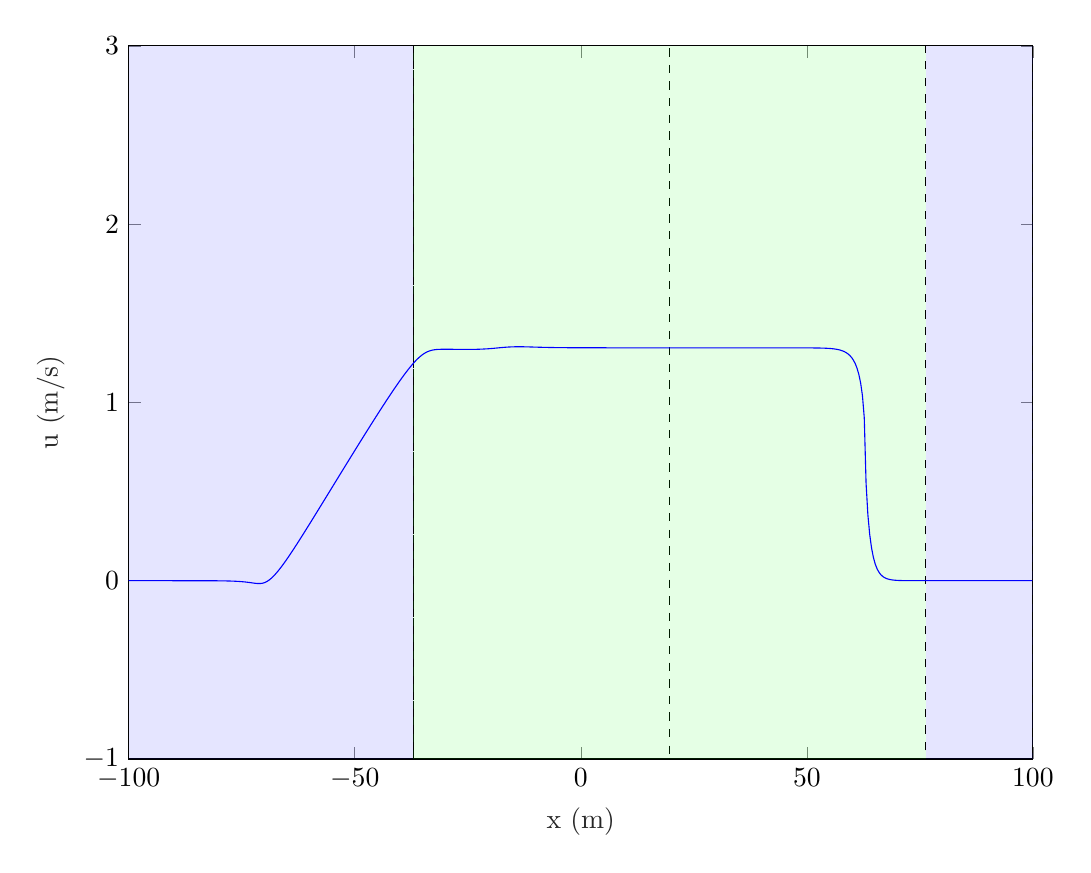
\begin{tikzpicture}

\begin{axis}[%
width=4.521in,
height=3.566in,
at={(0.758in,0.481in)},
scale only axis,
xmin=-100,
xmax=100,
xtick={-100,  -50,    0,   50,  100},
xlabel style={font=\color{white!15!black}},
xlabel={x (m)},
ymin=-1,
ymax=3,
ytick={-1,  0,  1,  2,  3},
ylabel style={font=\color{white!15!black}},
ylabel={u (m/s)},
axis background/.style={fill=white}
]

\addplot[area legend, dashed, draw=black, fill=blue, fill opacity=0.1, forget plot]
table[row sep=crcr] {%
x	y\\
-100	-3\\
-100	3\\
-37.0630892039997	3\\
-37.0630892039997	-3\\
}--cycle;

\addplot[area legend, dashed, draw=black, fill=green, fill opacity=0.1, forget plot]
table[row sep=crcr] {%
x	y\\
-37.0630892039997	-3\\
-37.0630892039997	3\\
19.5890566189392	3\\
19.5890566189392	-3\\
}--cycle;

\addplot[area legend, draw=none, fill=green, fill opacity=0.1, forget plot]
table[row sep=crcr] {%
x	y\\
19.5890566189392	-3\\
19.5890566189392	3\\
76.2412024418781	3\\
76.2412024418781	-3\\
}--cycle;

\addplot[area legend, dashed, draw=black, fill=blue, fill opacity=0.1, forget plot]
table[row sep=crcr] {%
x	y\\
76.2412024418781	-3\\
76.2412024418781	3\\
100	3\\
100	-3\\
}--cycle;
\addplot [color=blue, forget plot]
  table[row sep=crcr]{%
-100.1200120012	0\\
-99.7199719971997	-1.36171330571723e-08\\
-99.3199319931993	-3.86043806432635e-08\\
-98.9198919891989	-8.04975401171462e-08\\
-98.5198519851985	-1.38006123441225e-07\\
-98.1198119811981	-2.10622955427693e-07\\
-97.7197719771977	-2.98555252660792e-07\\
-97.3197319731973	-4.02682967512809e-07\\
-96.9196919691969	-5.24542429009571e-07\\
-96.5196519651965	-6.66333465819747e-07\\
-96.1196119611961	-8.30949463735897e-07\\
-95.7195719571957	-1.022030449519e-06\\
-95.3195319531953	-1.24403957285489e-06\\
-94.9194919491949	-1.50236492257496e-06\\
-94.5194519451945	-1.80344875481825e-06\\
-94.1194119411941	-2.1549471332124e-06\\
-93.7193719371937	-2.56592389178225e-06\\
-93.3193319331933	-3.04708390420881e-06\\
-92.9192919291929	-3.6110516196321e-06\\
-92.5192519251925	-4.27270215084885e-06\\
-92.1192119211921	-5.04955342506242e-06\\
-91.7191719171917	-5.96223002559332e-06\\
-91.3191319131913	-7.03501072124817e-06\\
-90.9190919091909	-8.29647436252028e-06\\
-90.5190519051905	-9.78026134951059e-06\\
-90.1190119011901	-1.15259708949269e-05\\
-89.7189718971897	-1.35802183437606e-05\\
-89.3189318931893	-1.59978801293247e-05\\
-88.9188918891889	-1.88435604834424e-05\\
-88.5188518851885	-2.21933185600337e-05\\
-88.1188118811881	-2.61367024222989e-05\\
-87.7187718771877	-3.07791439252042e-05\\
-87.3187318731873	-3.62447789094053e-05\\
-86.9186918691869	-4.26797682031923e-05\\
-86.5186518651865	-5.02562084076841e-05\\
-86.1186118611861	-5.917673678217e-05\\
-85.7185718571857	-6.96799529770825e-05\\
-85.3185318531853	-8.20468029100796e-05\\
-84.9184918491849	-9.66080938311674e-05\\
-84.5184518451845	-0.000113753340524898\\
-84.1184118411841	-0.000133941176694241\\
-83.7183718371837	-0.000157711604886564\\
-83.3183318331833	-0.000185700405005864\\
-82.9182918291829	-0.000218656075327844\\
-82.5182518251825	-0.000257459732906049\\
-82.1182118211821	-0.000303148480898846\\
-81.7181718171817	-0.000356942806670754\\
-81.3181318131813	-0.000420278656432083\\
-80.9180918091809	-0.000494844920789905\\
-80.5180518051805	-0.000582627104643179\\
-80.1180118011801	-0.000685958027456381\\
-79.7179717971797	-0.000807576387199764\\
-79.3179317931793	-0.000950693903684012\\
-78.9178917891789	-0.00111907161214939\\
-78.5178517851785	-0.00131710540167639\\
-78.1178117811781	-0.00154991959956249\\
-77.7177717771777	-0.001823466705717\\
-77.3177317731773	-0.0021446273134496\\
-76.9176917691769	-0.00252130180129145\\
-76.5176517651765	-0.00296247620978857\\
-76.1176117611761	-0.00347823169500986\\
-75.7175717571757	-0.00407965331404072\\
-75.3175317531753	-0.00477855131919683\\
-74.9174917491749	-0.00558688046485275\\
-74.5174517451745	-0.00651561929822068\\
-74.1174117411741	-0.00757280829700939\\
-73.7173717371737	-0.00876026431641017\\
-73.3173317331733	-0.010068271788174\\
-72.9172917291729	-0.0114675054025247\\
-72.5172517251725	-0.0128976141713181\\
-72.1172117211721	-0.0142530890217991\\
-71.7171717171717	-0.0153695509875106\\
-71.3171317131713	-0.0160160068056466\\
-70.9170917091709	-0.015886321551575\\
-70.5170517051705	-0.014709754355048\\
-70.1170117011701	-0.0122265821941101\\
-69.7169716971697	-0.00827727550621283\\
-69.3169316931693	-0.00281672567331452\\
-68.9168916891689	0.00410068295348886\\
-68.5168516851685	0.0123570167584396\\
-68.1168116811681	0.0218045262843995\\
-67.7167716771677	0.0322898398979848\\
-67.3167316731673	0.0436679298934694\\
-66.9166916691669	0.0558085608486784\\
-66.5166516651665	0.0685982097425687\\
-66.1166116611661	0.0819396226282433\\
-65.7165716571657	0.0957502485750918\\
-65.3165316531653	0.109960265218244\\
-64.9164916491649	0.124510736621502\\
-64.5164516451645	0.139351996481014\\
-64.1164116411641	0.154442097613106\\
-63.7163716371637	0.169745494872318\\
-63.3163316331633	0.185232044578884\\
-62.9162916291629	0.200876118957862\\
-62.5162516251625	0.216655838092714\\
-62.1162116211621	0.232552481389314\\
-61.7161716171617	0.248549987605756\\
-61.3161316131613	0.26463452996825\\
-60.9160916091609	0.280794163934023\\
-60.5160516051605	0.297018526981761\\
-60.1160116011601	0.313298612814737\\
-59.7159715971597	0.3296265569622\\
-59.3159315931593	0.345995472871744\\
-58.9158915891589	0.362399301344585\\
-58.5158515851585	0.37883268984894\\
-58.1158115811581	0.395290888486583\\
-57.7157715771577	0.411769651657719\\
-57.3157315731573	0.42826517932391\\
-56.9156915691569	0.444774051186768\\
-56.5156515651565	0.461293165387447\\
-56.1156115611561	0.477819685396676\\
-55.7155715571557	0.494351004496086\\
-55.3155315531553	0.510884710379248\\
-54.9154915491549	0.527418553648154\\
-54.5154515451545	0.543950421211407\\
-54.1154115411541	0.560478307344351\\
-53.7153715371537	0.577000296944458\\
-53.3153315331533	0.593514553063535\\
-52.9152915291529	0.610019271359759\\
-52.5152515251525	0.626512678349658\\
-52.1152115211521	0.642993020275486\\
-51.7151715171517	0.659458554308463\\
-51.3151315131513	0.675907527854866\\
-50.9150915091509	0.692338150165155\\
-50.5150515051505	0.708748595050329\\
-50.1150115011501	0.72513699391489\\
-49.7149714971497	0.741501402372227\\
-49.3149314931493	0.757839785971804\\
-48.9148914891489	0.774150006251962\\
-48.5148514851485	0.790429804260773\\
-48.1148114811481	0.80667677830861\\
-47.7147714771477	0.822888360464731\\
-47.3147314731473	0.839061804704002\\
-46.9146914691469	0.855194114367692\\
-46.5146514651465	0.871282036869743\\
-46.1146114611461	0.887322038197265\\
-45.7145714571457	0.903310251927707\\
-45.3145314531453	0.919242403505617\\
-44.9144914491449	0.935113791699767\\
-44.5144514451445	0.950919197805741\\
-44.1144114411441	0.966652793123028\\
-43.7143714371437	0.982308052800139\\
-43.3143314331433	0.997877647327927\\
-42.9142914291429	1.01335330320316\\
-42.5142514251425	1.02872566114121\\
-42.1142114211421	1.04398404686152\\
-41.7141714171417	1.05911626175097\\
-41.3141314131413	1.07410835349761\\
-40.9140914091409	1.08894427764597\\
-40.5140514051405	1.1036055290507\\
-40.1140114011401	1.11807073729612\\
-39.7139713971397	1.13231511837756\\
-39.3139313931393	1.14630990250235\\
-38.9138913891389	1.16002167535151\\
-38.5138513851385	1.17341163797752\\
-38.1138113811381	1.18643483823492\\
-37.7137713771377	1.19903933276213\\
-37.3137313731373	1.21116559048393\\
-36.9136913691369	1.2227460928362\\
-36.5136513651365	1.23370544637946\\
-36.1136113611361	1.24396153923479\\
-35.7135713571357	1.25342821322674\\
-35.3135313531353	1.26202001133514\\
-34.9134913491349	1.2696596669195\\
-34.5134513451345	1.27628826160699\\
-34.1134113411341	1.28187672477457\\
-33.7133713371337	1.2864362319037\\
-33.3133313331333	1.29002344826919\\
-32.9132913291329	1.2927372291745\\
-32.5132513251325	1.29470660115615\\
-32.1132113211321	1.29607365447\\
-31.7131713171317	1.29697663076977\\
-31.3131313131313	1.29753776731952\\
-30.9130913091309	1.29785729722206\\
-30.5130513051305	1.29801267712639\\
-30.1130113011301	1.29806134834703\\
-29.7129712971297	1.29804573363\\
-29.3129312931293	1.2979904808609\\
-28.9128912891289	1.29791461408359\\
-28.5128512851285	1.29783040836197\\
-28.1128112811281	1.29774530300629\\
-27.7127712771277	1.29766348331168\\
-27.3127312731273	1.29758714164345\\
-26.9126912691269	1.29751728400211\\
-26.5126512651265	1.29745439792691\\
-26.1126112611261	1.29739896519396\\
-25.7125712571257	1.2973523057046\\
-25.3125312531253	1.29731751136779\\
-24.9124912491249	1.29729815895551\\
-24.5124512451245	1.29730086978518\\
-24.1124112411241	1.29734118451849\\
-23.7123712371237	1.2974334813017\\
-23.3123312331233	1.29759224988726\\
-22.9122912291229	1.29783403250708\\
-22.5122512251225	1.29816957767483\\
-22.1122112211221	1.29858646688119\\
-21.7121712171217	1.29906388993883\\
-21.3121312131213	1.2995831525355\\
-20.9120912091209	1.30012706319379\\
-20.5120512051205	1.3007434507105\\
-20.1120112011201	1.30147484163172\\
-19.7119711971197	1.30230757775694\\
-19.3119311931193	1.30321720854923\\
-18.9118911891189	1.30417449291115\\
-18.5118511851185	1.30515926233934\\
-18.1118111811181	1.30615029785144\\
-17.7117711771177	1.3071212877184\\
-17.3117311731173	1.30804781425408\\
-16.9116911691169	1.30890919113453\\
-16.5116511651165	1.30966802741225\\
-16.1116111611161	1.31031020365086\\
-15.7115711571157	1.31085036798933\\
-15.3115311531153	1.31129703952755\\
-14.9114911491149	1.3116489312749\\
-14.5114511451145	1.31189967332021\\
-14.1114111411141	1.31204875584652\\
-13.7113711371137	1.31210386462291\\
-13.3113311331133	1.31207520208519\\
-12.9112911291129	1.31195857831955\\
-12.5112511251125	1.31178122784604\\
-12.1112111211121	1.31155309211496\\
-11.7111711171117	1.311287967525\\
-11.3111311131113	1.31099870856652\\
-10.9110911091109	1.31069463826987\\
-10.5110511051105	1.31038430709834\\
-10.1110111011101	1.3100745832335\\
-9.71097109710971	1.3097698659421\\
-9.3109310931093	1.30947543729885\\
-8.9108910891089	1.30919384080678\\
-8.51085108510851	1.30892707850205\\
-8.11081108110811	1.30867627576183\\
-7.71077107710771	1.30844238868218\\
-7.31073107310731	1.30822514378913\\
-6.9106910691069	1.30802419066444\\
-6.5106510651065	1.30783920559733\\
-6.11061106110611	1.30766960896346\\
-5.71057105710571	1.30751478489634\\
-5.31053105310531	1.30737383706792\\
-4.91049104910491	1.30724570687505\\
-4.5104510451045	1.30713009206782\\
-4.1104110411041	1.30702571045423\\
-3.71037103710371	1.30693185180739\\
-3.31033103310331	1.30684749529184\\
-2.91029102910291	1.306772013029\\
-2.51025102510251	1.30670448237732\\
-2.1102110211021	1.3066446034709\\
-1.7101710171017	1.30659071698232\\
-1.31013101310131	1.30654269515539\\
-0.91009100910091	1.30650046075505\\
-0.510051005100507	1.30646326773523\\
-0.110011001100105	1.30643031365145\\
0.290029002900297	1.30640094289514\\
0.6900690069007	1.30637447446724\\
1.09010901090109	1.30635045056298\\
1.49014901490149	1.30632899804495\\
1.89018901890189	1.30631025398762\\
2.2902290229023	1.3062928967614\\
2.6902690269027	1.30627722058156\\
3.0903090309031	1.30626294161484\\
3.4903490349035	1.30624970317645\\
3.89038903890389	1.30623729476897\\
4.29042904290429	1.30622547657624\\
4.6904690469047	1.30621445084177\\
5.0905090509051	1.30620392660863\\
5.4905490549055	1.30619349069495\\
5.8905890589059	1.30618344558524\\
6.29062906290629	1.30617351426755\\
6.69066906690669	1.30616339388514\\
7.0907090709071	1.30615412599259\\
7.4907490749075	1.30614463087681\\
7.8907890789079	1.30613488811394\\
8.2908290829083	1.30612550985341\\
8.69086908690869	1.30611635302175\\
9.09090909090909	1.30610718538575\\
9.4909490949095	1.30609787192925\\
9.8909890989099	1.30608850139001\\
10.2910291029103	1.30607916768018\\
10.6910691069107	1.30606990708435\\
11.0911091109111	1.30606092104798\\
11.4911491149115	1.30605228109639\\
11.8911891189119	1.30604412171324\\
12.2912291229123	1.30603622897271\\
12.6912691269127	1.30602837193058\\
13.0913091309131	1.30602009282422\\
13.4913491349135	1.30601195110115\\
13.8913891389139	1.30600445122916\\
14.2914291429143	1.30599744212491\\
14.6914691469147	1.30599020291133\\
15.0915091509151	1.30598302125373\\
15.4915491549155	1.3059765297833\\
15.8915891589159	1.30597006546405\\
16.2916291629163	1.30596378761825\\
16.6916691669167	1.30595789422944\\
17.0917091709171	1.30595208148469\\
17.4917491749175	1.30594658815184\\
17.8917891789179	1.30594128234211\\
18.2918291829183	1.30593616255734\\
18.6918691869187	1.30593136066741\\
19.0919091909191	1.30592669792157\\
19.4919491949195	1.30592226970357\\
19.8919891989199	1.30591811047888\\
20.2920292029203	1.30591407731974\\
20.6920692069207	1.30591035130839\\
21.0921092109211	1.3059066972825\\
21.4921492149215	1.30590337234401\\
21.8921892189219	1.30590001444331\\
22.2922292229223	1.3058970929837\\
22.6922692269227	1.30589408263949\\
23.0923092309231	1.30589140798406\\
23.4923492349235	1.305888805762\\
23.8923892389239	1.30588635775237\\
24.2924292429243	1.30588404987005\\
24.6924692469247	1.30588183103099\\
25.0925092509251	1.30587988581926\\
25.4925492549255	1.30587782058843\\
25.8925892589259	1.30587596025679\\
26.2926292629263	1.30587419745831\\
26.6926692669267	1.3058724761933\\
27.0927092709271	1.30587096707484\\
27.4927492749275	1.30586924903943\\
27.8927892789279	1.30586778062825\\
28.2928292829283	1.30586652515237\\
28.6928692869287	1.30586521283818\\
29.0929092909291	1.30586403218052\\
29.4929492949295	1.30586275130919\\
29.8929892989299	1.30586144048134\\
30.2930293029303	1.30586031903266\\
30.6930693069307	1.30585933295475\\
31.0931093109311	1.30585835237561\\
31.4931493149315	1.30585747937048\\
31.8931893189319	1.30585642883725\\
32.2932293229323	1.30585535931712\\
32.6932693269327	1.30585444450463\\
33.0933093309331	1.30585355677607\\
33.4933493349335	1.30585261352497\\
33.8933893389339	1.30585187330464\\
34.2934293429343	1.30585117803793\\
34.6934693469347	1.30585045195143\\
35.0935093509351	1.30584978438007\\
35.4935493549355	1.30584906851966\\
35.8935893589359	1.30584818222258\\
36.2936293629363	1.30584736896821\\
36.6936693669367	1.30584669088016\\
37.0937093709371	1.30584595403048\\
37.4937493749375	1.30584513280684\\
37.8937893789379	1.30584443476043\\
38.2938293829383	1.30584379390605\\
38.6938693869387	1.305843211875\\
39.0939093909391	1.30584272460557\\
39.4939493949395	1.30584216846799\\
39.8939893989399	1.30584141908997\\
40.2940294029403	1.30584073353521\\
40.6940694069407	1.30584014287055\\
41.0941094109411	1.30583931782403\\
41.4941494149415	1.30583824587012\\
41.8941894189419	1.3058374230843\\
42.2942294229423	1.30583653811662\\
42.6942694269427	1.30583535535079\\
43.0943094309431	1.30583380511927\\
43.4943494349435	1.30583240289405\\
43.8943894389439	1.30583072096629\\
44.2944294429443	1.3058286407365\\
44.6944694469447	1.30582595803827\\
45.0945094509451	1.30582315623874\\
45.4945494549455	1.30581958413422\\
45.8945894589459	1.30581530836768\\
46.2946294629463	1.30580977976536\\
46.6946694669467	1.30580340965401\\
47.0947094709471	1.30579520706555\\
47.4947494749475	1.3057853939333\\
47.8947894789479	1.30577271808929\\
48.2948294829483	1.30575742270188\\
48.6948694869487	1.30573792775973\\
49.0949094909491	1.30571422311038\\
49.4949494949495	1.30568390306491\\
49.8949894989499	1.30564664994452\\
50.2950295029503	1.30559949408586\\
50.6950695069507	1.3055413486637\\
51.0951095109511	1.30546760949675\\
51.4951495149515	1.30537619411716\\
51.8951895189519	1.30526095081423\\
52.2952295229523	1.30511766004889\\
52.6952695269527	1.30493722351941\\
53.0953095309531	1.30471218104175\\
53.4953495349535	1.30442974365222\\
53.8953895389539	1.30407680899638\\
54.2954295429543	1.30363367813601\\
54.6954695469547	1.30307889080148\\
55.0955095509551	1.30238319443149\\
55.4955495549555	1.30151083845052\\
55.8955895589559	1.30041606286762\\
56.2956295629563	1.29904092060112\\
56.6956695669567	1.29731419140536\\
57.0957095709571	1.29514059939439\\
57.4957495749575	1.29240562404719\\
57.8957895789579	1.28895361089113\\
58.2958295829583	1.28459622005019\\
58.6958695869587	1.27907160496474\\
59.0959095909591	1.27205731483877\\
59.4959495949595	1.26309835099228\\
59.8959895989599	1.25161286494192\\
60.2960296029603	1.23675622701038\\
60.6960696069607	1.21737476686809\\
61.0961096109611	1.19170128613847\\
61.4961496149615	1.15702855108909\\
61.8961896189619	1.10862216015684\\
62.2962296229623	1.03713084931818\\
62.6962696269627	0.914464252767662\\
63.0963096309631	0.546360188604767\\
63.4963496349635	0.36969938549438\\
63.8963896389639	0.260198279873676\\
64.2964296429643	0.185397595948234\\
64.6964696469647	0.132819149251402\\
65.0965096509651	0.0954149610904409\\
65.4965496549655	0.0686494940744014\\
65.8965896589659	0.0494367882329877\\
66.2966296629663	0.035620929130273\\
66.6966696669667	0.0256752853514982\\
67.0967096709671	0.0185108985144953\\
67.4967496749675	0.0133477664042973\\
67.8967896789679	0.00962580216270394\\
68.2968296829683	0.00694221547779605\\
68.6968696869687	0.00500705410059942\\
69.0969096909691	0.0036114596350305\\
69.4969496949695	0.00260492260290376\\
69.8969896989699	0.0018789496664515\\
70.2970297029703	0.00135531855274367\\
70.6970697069707	0.000977624019435061\\
71.0971097109711	0.000705188776331408\\
71.4971497149715	0.000508675841517402\\
71.8971897189719	0.000366925936360138\\
72.2972297229723	0.000264677392115959\\
72.6972697269727	0.000190922055606672\\
73.0973097309731	0.000137719661594194\\
73.4973497349735	9.93427591135527e-05\\
73.8973897389739	7.16599986414401e-05\\
74.2974297429743	5.16913166960216e-05\\
74.6974697469747	3.72870953647737e-05\\
75.0975097509751	2.68967388923863e-05\\
75.4975497549755	1.94017445830848e-05\\
75.8975897589759	1.39952930948855e-05\\
76.2976297629763	1.00953935770774e-05\\
76.6976697669767	7.28223249839232e-06\\
77.0977097709771	5.25298115475737e-06\\
77.4977497749775	3.78919674161794e-06\\
77.8977897789779	2.73330737405993e-06\\
78.2978297829783	1.97164986360399e-06\\
78.6978697869787	1.42223419444387e-06\\
79.0979097909791	1.02591751606183e-06\\
79.4979497949795	7.40037590017949e-07\\
79.8979897989799	5.33820332413481e-07\\
80.2980298029803	3.85067123324701e-07\\
80.6980698069807	2.7776515873709e-07\\
81.0981098109811	2.00363734704925e-07\\
81.4981498149815	1.44530816035368e-07\\
81.8981898189819	1.04256179854388e-07\\
82.2982298229823	7.52043831553822e-08\\
82.6982698269827	5.42480868572422e-08\\
83.0983098309831	3.91314400579005e-08\\
83.4983498349835	2.82271488172564e-08\\
83.8983898389839	2.03614193640036e-08\\
84.2984298429843	1.46875441719418e-08\\
84.6984698469847	1.05947302905875e-08\\
85.0985098509851	7.64241197982609e-09\\
85.4985498549855	5.51278329342288e-09\\
85.8985898589859	3.97659828881677e-09\\
86.2986298629863	2.86847910083268e-09\\
86.6986698669867	2.0691465880023e-09\\
87.0987098709871	1.49256856042892e-09\\
87.4987498749875	1.07666344872009e-09\\
87.8987898789879	7.76651805187819e-10\\
88.2988298829883	5.60235241044423e-10\\
88.6988698869887	4.04124658607196e-10\\
89.0989098909891	2.91517110863795e-10\\
89.4989498949895	2.10281695304606e-10\\
89.8989898989899	1.51694563744997e-10\\
90.2990299029903	1.09430048036066e-10\\
90.6990699069907	7.893258391629e-11\\
91.0991099109911	5.69371138366473e-11\\
91.4991499149915	4.10753532842825e-11\\
91.8991899189919	2.96276589584885e-11\\
92.2992299229923	2.13692427966522e-11\\
92.6992699269927	1.54190489397807e-11\\
93.0993099309931	1.11228477333938e-11\\
93.4993499349935	8.03355106204337e-12\\
93.8993899389939	5.79892708741824e-12\\
94.2994299429943	4.19050215363533e-12\\
94.6994699469947	3.01586031402374e-12\\
95.0995099509951	2.17896595531011e-12\\
95.4995499549955	1.57057653828411e-12\\
95.8995899589959	1.13143978435305e-12\\
96.2996299629963	8.0805115739175e-13\\
96.6996699669967	5.81542528359101e-13\\
97.0997099709971	4.17480626204375e-13\\
97.4997499749975	2.9655542244862e-13\\
97.8997899789979	2.12013220487956e-13\\
98.2998299829983	1.42711137911824e-13\\
98.6998699869987	9.29995763623602e-14\\
99.0999099909991	5.67556346952496e-14\\
99.4999499949995	2.36247095143087e-14\\
99.8999899989999	3.35605205513114e-15\\
};
\end{axis}
\end{tikzpicture}%
		\caption{$u$}
	\end{subfigure}
	\caption{Solution of gSGN with $\beta_1 = 3 -\dfrac{2}{3} $ and $\beta_2 = 3$ (Regularised Shallow Water Wave Equations) for smooth dam-break problem at $t=15s$ with inequality regions shown.}
	\label{fig:RegSWWESDB}
\end{figure}

\begin{figure}
	\tikzset{every picture/.style={scale=0.75}}%
	\centering
	\begin{subfigure}{0.49\textwidth}
		\centering
		% This file was created by matlab2tikz.
%
%The latest updates can be retrieved from
%  http://www.mathworks.com/matlabcentral/fileexchange/22022-matlab2tikz-matlab2tikz
%where you can also make suggestions and rate matlab2tikz.
%
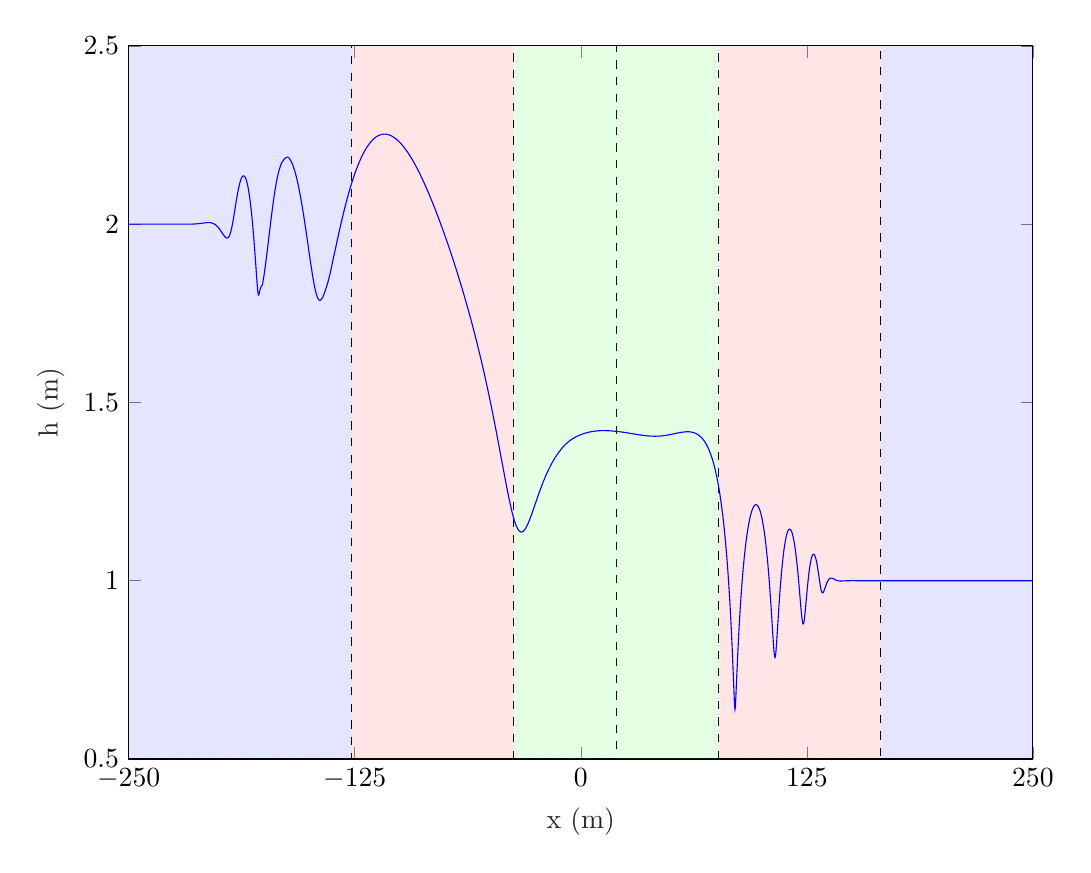
\begin{tikzpicture}

\begin{axis}[%
width=4.521in,
height=3.566in,
at={(0.758in,0.481in)},
scale only axis,
xmin=-250,
xmax=250,
xtick={-250, -125,    0,  125,  250},
xlabel style={font=\color{white!15!black}},
xlabel={x (m)},
ymin=0.5,
ymax=2.5,
ytick={0.5,   1, 1.5,   2, 2.5},
ylabel style={font=\color{white!15!black}},
ylabel={h (m)},
axis background/.style={fill=white}
]

\addplot[area legend, dashed, draw=black, fill=blue, fill opacity=0.1, forget plot]
table[row sep=crcr] {%
x	y\\
-250	0.5\\
-250	2.5\\
-126.679671409596	2.5\\
-126.679671409596	0.5\\
}--cycle;

\addplot[area legend, draw=none, fill=red, fill opacity=0.1, forget plot]
table[row sep=crcr] {%
x	y\\
-126.679671409596	0.5\\
-126.679671409596	2.5\\
-37.0611924008642	2.5\\
-37.0611924008642	0.5\\
}--cycle;

\addplot[area legend, dashed, draw=black, fill=green, fill opacity=0.1, forget plot]
table[row sep=crcr] {%
x	y\\
-37.0611924008642	0.5\\
-37.0611924008642	2.5\\
19.5880540963537	2.5\\
19.5880540963537	0.5\\
}--cycle;

\addplot[area legend, draw=none, fill=green, fill opacity=0.1, forget plot]
table[row sep=crcr] {%
x	y\\
19.5880540963537	0.5\\
19.5880540963537	2.5\\
76.2373005935716	2.5\\
76.2373005935716	0.5\\
}--cycle;

\addplot[area legend, dashed, draw=black, fill=red, fill opacity=0.1, forget plot]
table[row sep=crcr] {%
x	y\\
76.2373005935716	0.5\\
76.2373005935716	2.5\\
165.855779602303	2.5\\
165.855779602303	0.5\\
}--cycle;

\addplot[area legend, draw=none, fill=blue, fill opacity=0.1, forget plot]
table[row sep=crcr] {%
x	y\\
165.855779602303	0.5\\
165.855779602303	2.5\\
250	2.5\\
250	0.5\\
}--cycle;
\addplot [color=blue, forget plot]
  table[row sep=crcr]{%
-250.100003333444	2\\
-249.933331111037	1.99999999561396\\
-249.76665888863	1.99999998856255\\
-249.599986666222	1.99999998219928\\
-249.433314443815	1.99999997653527\\
-249.266642221407	1.999999971582\\
-249.099969999	1.99999996735178\\
-248.933297776593	1.99999996385771\\
-248.766625554185	1.99999996111384\\
-248.599953331778	1.99999995913517\\
-248.43328110937	1.99999995793774\\
-248.266608886963	1.99999995753954\\
-248.099936664555	1.99999995795543\\
-247.933264442148	1.99999995920815\\
-247.766592219741	1.99999996131775\\
-247.599919997333	1.99999996430622\\
-247.433247774926	1.99999996819686\\
-247.266575552518	1.99999997301436\\
-247.099903330111	1.99999997878474\\
-246.933231107704	1.9999999855354\\
-246.766558885296	1.99999999329519\\
-246.599886662889	2.00000000209438\\
-246.433214440481	2.00000001196467\\
-246.266542218074	2.0000000229392\\
-246.099869995667	2.00000003505254\\
-245.933197773259	2.00000004834069\\
-245.766525550852	2.00000006284108\\
-245.599853328444	2.0000000785925\\
-245.433181106037	2.00000009563512\\
-245.266508883629	2.00000011401043\\
-245.099836661222	2.00000013376121\\
-244.933164438815	2.00000015493146\\
-244.766492216407	2.00000017756636\\
-244.599819994	2.00000020171218\\
-244.433147771592	2.00000022741623\\
-244.266475549185	2.00000025472673\\
-244.099803326778	2.00000028369275\\
-243.93313110437	2.00000031436408\\
-243.766458881963	2.00000034679114\\
-243.599786659555	2.00000038102474\\
-243.433114437148	2.00000041711605\\
-243.26644221474	2.00000045511644\\
-243.099769992333	2.00000049507722\\
-242.933097769926	2.00000053704947\\
-242.766425547518	2.00000058108389\\
-242.599753325111	2.00000062723054\\
-242.433081102703	2.00000067553857\\
-242.266408880296	2.00000072605601\\
-242.099736657889	2.00000077882947\\
-241.933064435481	2.00000083390386\\
-241.766392213074	2.00000089132205\\
-241.599719990666	2.00000095112453\\
-241.433047768259	2.00000101334908\\
-241.266375545852	2.00000107803034\\
-241.099703323444	2.00000114519945\\
-240.933031101037	2.00000121488355\\
-240.766358878629	2.00000128710537\\
-240.599686656222	2.00000136188273\\
-240.433014433814	2.00000143922802\\
-240.266342211407	2.00000151914765\\
-240.099669989	2.00000160164146\\
-239.932997766592	2.00000168670212\\
-239.766325544185	2.00000177431459\\
-239.599653321777	2.00000186445532\\
-239.43298109937	2.00000195709158\\
-239.266308876963	2.00000205218074\\
-239.099636654555	2.00000214966949\\
-238.932964432148	2.00000224949301\\
-238.76629220974	2.00000235157412\\
-238.599619987333	2.00000245582251\\
-238.432947764926	2.00000256213364\\
-238.266275542518	2.00000267038789\\
-238.099603320111	2.00000278044955\\
-237.932931097703	2.00000289216579\\
-237.766258875296	2.00000300536556\\
-237.599586652888	2.0000031198584\\
-237.432914430481	2.0000032354334\\
-237.266242208074	2.00000335185798\\
-237.099569985666	2.00000346887662\\
-236.932897763259	2.00000358620963\\
-236.766225540851	2.00000370355176\\
-236.599553318444	2.00000382057088\\
-236.432881096037	2.00000393690655\\
-236.266208873629	2.00000405217016\\
-236.099536651222	2.00000416593797\\
-235.932864428814	2.00000427775767\\
-235.766192206407	2.00000438714163\\
-235.599519983999	2.00000449356466\\
-235.432847761592	2.00000459646702\\
-235.266175539185	2.00000469524833\\
-235.099503316777	2.00000478926856\\
-234.93283109437	2.000004877845\\
-234.766158871962	2.00000496025149\\
-234.599486649555	2.0000050357162\\
-234.432814427148	2.00000510342023\\
-234.26614220474	2.00000516249587\\
-234.099469982333	2.00000521202502\\
-233.932797759925	2.00000525103747\\
-233.766125537518	2.00000527850916\\
-233.599453315111	2.00000529336085\\
-233.432781092703	2.00000529446516\\
-233.266108870296	2.00000528065328\\
-233.099436647888	2.00000525064188\\
-232.932764425481	2.0000052031113\\
-232.766092203073	2.00000513668323\\
-232.599419980666	2.00000504991509\\
-232.432747758259	2.00000494129911\\
-232.266075535851	2.00000480926214\\
-232.099403313444	2.00000465216377\\
-231.932731091036	2.00000446829509\\
-231.766058868629	2.00000425587875\\
-231.599386646222	2.00000401306916\\
-231.432714423814	2.00000373795065\\
-231.266042201407	2.0000034285379\\
-231.099369978999	2.00000308277716\\
-230.932697756592	2.00000269854456\\
-230.766025534184	2.00000227364822\\
-230.599353311777	2.0000018058297\\
-230.43268108937	2.00000129276239\\
-230.266008866962	2.00000073205676\\
-230.099336644555	2.00000012125847\\
-229.932664422147	1.99999945785429\\
-229.76599219974	1.99999873927131\\
-229.599319977333	1.9999979628831\\
-229.432647754925	1.99999712600988\\
-229.265975532518	1.99999622592587\\
-229.09930331011	1.99999525986215\\
-228.932631087703	1.99999422501603\\
-228.765958865296	1.99999311854363\\
-228.599286642888	1.99999193758235\\
-228.432614420481	1.99999067925293\\
-228.265942198073	1.99998934065652\\
-228.099269975666	1.99998791889933\\
-227.932597753258	1.99998641109202\\
-227.765925530851	1.99998481435941\\
-227.599253308444	1.99998312585686\\
-227.432581086036	1.99998134277842\\
-227.265908863629	1.99997946236959\\
-227.099236641221	1.99997748194026\\
-226.932564418814	1.99997539888147\\
-226.765892196407	1.99997321068102\\
-226.599219973999	1.99997091493817\\
-226.432547751592	1.999968509383\\
-226.265875529184	1.9999659918955\\
-226.099203306777	1.99996336052512\\
-225.932531084369	1.99996061351339\\
-225.765858861962	1.99995774931674\\
-225.599186639555	1.99995476662926\\
-225.432514417147	1.99995166440939\\
-225.26584219474	1.99994844190819\\
-225.099169972332	1.99994509869384\\
-224.932497749925	1.99994163468513\\
-224.765825527518	1.99993805018078\\
-224.59915330511	1.99993434589409\\
-224.432481082703	1.99993052298574\\
-224.265808860295	1.99992658309976\\
-224.099136637888	1.99992252840315\\
-223.932464415481	1.99991836162635\\
-223.765792193073	1.99991408609091\\
-223.599119970666	1.9999097057596\\
-223.432447748258	1.99990522529554\\
-223.265775525851	1.99990065008758\\
-223.099103303443	1.99989598630035\\
-222.932431081036	1.99989124092859\\
-222.765758858629	1.9998864218414\\
-222.599086636221	1.99988153783478\\
-222.432414413814	1.99987659868361\\
-222.265742191406	1.99987161519669\\
-222.099069968999	1.99986659927421\\
-221.932397746592	1.99986156395882\\
-221.765725524184	1.99985652348358\\
-221.599053301777	1.99985149333556\\
-221.432381079369	1.99984649033986\\
-221.265708856962	1.9998415326796\\
-221.099036634554	1.99983663996469\\
-220.932364412147	1.99983183330721\\
-220.76569218974	1.99982713536448\\
-220.599019967332	1.99982257039998\\
-220.432347744925	1.9998181643477\\
-220.265675522517	1.99981394486428\\
-220.09900330011	1.99980994137998\\
-219.932331077703	1.99980618516275\\
-219.765658855295	1.99980270936309\\
-219.598986632888	1.99979954906892\\
-219.43231441048	1.9997967413504\\
-219.265642188073	1.9997943253025\\
-219.098969965666	1.99979234208999\\
-218.932297743258	1.99979083498214\\
-218.765625520851	1.99978984938569\\
-218.598953298443	1.99978943316905\\
-218.432281076036	1.99978963402948\\
-218.265608853628	1.99979050484725\\
-218.098936631221	1.99979210039596\\
-217.932264408814	1.99979447709102\\
-217.765592186406	1.99979769356343\\
-217.598919963999	1.99980181046893\\
-217.432247741591	1.99980689077286\\
-217.265575519184	1.9998129994218\\
-217.098903296777	1.99982020353342\\
-216.932231074369	1.99982857210549\\
-216.765558851962	1.99983817615968\\
-216.598886629554	1.99984908850838\\
-216.432214407147	1.99986138365733\\
-216.26554218474	1.9998751377898\\
-216.098869962332	1.9998904284523\\
-215.932197739925	1.99990733456682\\
-215.765525517517	1.99992593614222\\
-215.59885329511	1.99994631408202\\
-215.432181072702	1.99996855003045\\
-215.265508850295	1.9999927260424\\
-215.098836627888	2.00001892437491\\
-214.93216440548	2.00004722717198\\
-214.765492183073	2.00007771608262\\
-214.598819960665	2.00011047197976\\
-214.432147738258	2.00014557462551\\
-214.265475515851	2.00018310217683\\
-214.098803293443	2.00022313073287\\
-213.932131071036	2.00026573393825\\
-213.765458848628	2.00031098244534\\
-213.598786626221	2.00035894335317\\
-213.432114403813	2.00040967966433\\
-213.265442181406	2.00046324968888\\
-213.098769958999	2.00051970637179\\
-212.932097736591	2.00057909662529\\
-212.765425514184	2.00064146062183\\
-212.598753291776	2.00070683104768\\
-212.432081069369	2.00077523231671\\
-212.265408846962	2.00084667973923\\
-212.098736624554	2.00092117866766\\
-211.932064402147	2.0009987236071\\
-211.765392179739	2.00107929730711\\
-211.598719957332	2.0011628697868\\
-211.432047734924	2.00124939732785\\
-211.265375512517	2.001338821668\\
-211.09870329011	2.00143106910548\\
-210.932031067702	2.00152604825874\\
-210.765358845295	2.00162364960593\\
-210.598686622887	2.0017237451293\\
-210.43201440048	2.00182618710687\\
-210.265342178073	2.00193080657833\\
-210.098669955665	2.00203741118632\\
-209.931997733258	2.00214578594924\\
-209.76532551085	2.00225569075618\\
-209.598653288443	2.00236685989254\\
-209.431981066036	2.00247900065274\\
-209.265308843628	2.00259179239675\\
-209.098636621221	2.00270488541176\\
-208.931964398813	2.00281789998065\\
-208.765292176406	2.00293042537605\\
-208.598619953998	2.00304201894019\\
-208.431947731591	2.00315220523087\\
-208.265275509184	2.00326047523057\\
-208.098603286776	2.00336628567439\\
-207.931931064369	2.003469058447\\
-207.765258841961	2.00356818005918\\
-207.598586619554	2.00366300130782\\
-207.431914397147	2.00375283684853\\
-207.265242174739	2.00383696516538\\
-207.098569952332	2.00391462865\\
-206.931897729924	2.00398503359938\\
-206.765225507517	2.00404735052267\\
-206.598553285109	2.00410071481646\\
-206.431881062702	2.00414422724807\\
-206.265208840295	2.00417695482646\\
-206.098536617887	2.00419793237295\\
-205.93186439548	2.00420613632197\\
-205.765192173072	2.00420064823549\\
-205.598519950665	2.00418032450169\\
-205.431847728258	2.00414409678971\\
-205.26517550585	2.00409085699719\\
-205.098503283443	2.0040194810064\\
-204.931831061035	2.00392882401896\\
-204.765158838628	2.00381772591212\\
-204.598486616221	2.00368501572378\\
-204.431814393813	2.00352951375511\\
-204.265142171406	2.00335003570193\\
-204.098469948998	2.00314539764382\\
-203.931797726591	2.0029144201501\\
-203.765125504183	2.00265593349378\\
-203.598453281776	2.00236878282223\\
-203.431781059369	2.00205183400165\\
-203.265108836961	2.00170397962793\\
-203.098436614554	2.00132414539638\\
-202.931764392146	2.00091129698075\\
-202.765092169739	2.00046444735155\\
-202.598419947332	1.99998266445055\\
-202.431747724924	1.99946507924814\\
-202.265075502517	1.99891089420726\\
-202.098403280109	1.99831939247339\\
-201.931731057702	1.99768994769165\\
-201.765058835294	1.99702203387735\\
-201.598386612887	1.99631523586522\\
-201.43171439048	1.99556926066457\\
-201.265042168072	1.99478394951059\\
-201.098369945665	1.99395929058455\\
-200.931697723257	1.99309543157407\\
-200.76502550085	1.99219269399797\\
-200.598353278443	1.99125158771441\\
-200.431681056035	1.99027282695536\\
-200.265008833628	1.98925734757346\\
-200.09833661122	1.98820632431768\\
-199.931664388813	1.98712118721836\\
-199.764992166406	1.98600363934199\\
-199.598319943998	1.98485568042149\\
-199.431647721591	1.98367962854993\\
-199.264975499183	1.98247814156263\\
-199.098303276776	1.9812542393124\\
-198.931631054368	1.98001132929058\\
-198.764958831961	1.97875323299746\\
-198.598286609554	1.97748421144796\\
-198.431614387146	1.97620899288142\\
-198.264942164739	1.97493280150774\\
-198.098269942331	1.97366138528505\\
-197.931597719924	1.97240104527736\\
-197.764925497517	1.97115866396998\\
-197.598253275109	1.9699417333792\\
-197.431581052702	1.96875838017196\\
-197.264908830294	1.96761739025066\\
-197.098236607887	1.96652822875852\\
-196.93156438548	1.96550105461372\\
-196.764892163072	1.96454672958966\\
-196.598219940665	1.96367681859284\\
-196.431547718257	1.96290357457224\\
-196.26487549585	1.96223991966096\\
-196.098203273442	1.96169939803277\\
-195.931531051035	1.96129614448576\\
-195.764858828628	1.96104471965632\\
-195.59818660622	1.96096088893919\\
-195.431514383813	1.9610572890267\\
-195.264842161405	1.96135145500102\\
-195.098169938998	1.96185762372467\\
-194.931497716591	1.96259047422393\\
-194.764825494183	1.96356381890229\\
-194.598153271776	1.96479041011168\\
-194.431481049368	1.96628157036139\\
-194.264808826961	1.96804682739969\\
-194.098136604553	1.97009354857447\\
-193.931464382146	1.97242660142559\\
-193.764792159739	1.97504804651823\\
-193.598119937331	1.97795688823606\\
-193.431447714924	1.9811489086669\\
-193.264775492516	1.98461660641059\\
-193.098103270109	1.98834924802499\\
-192.931431047702	1.9923330166549\\
-192.764758825294	1.99655126317143\\
-192.598086602887	2.00098483809784\\
-192.431414380479	2.0056125032909\\
-192.264742158072	2.01041139108619\\
-192.098069935665	2.01535742777839\\
-191.931397713257	2.02042583118296\\
-191.76472549085	2.02559149957312\\
-191.598053268442	2.03082940575536\\
-191.431381046035	2.03611492002803\\
-191.264708823627	2.04142407760321\\
-191.09803660122	2.04673378691445\\
-190.931364378813	2.05202198648362\\
-190.764692156405	2.05726775240173\\
-190.598019933998	2.06245136110172\\
-190.43134771159	2.0675543204919\\
-190.264675489183	2.07255937222493\\
-190.098003266776	2.07745046740314\\
-189.931331044368	2.08221271931262\\
-189.764658821961	2.08683234436362\\
-189.597986599553	2.09129660922619\\
-189.431314377146	2.09559377256694\\
-189.264642154738	2.09971301457611\\
-189.097969932331	2.10364436466632\\
-188.931297709924	2.10737864045318\\
-188.764625487516	2.11090738075227\\
-188.597953265109	2.11422277811152\\
-188.431281042701	2.1173176383554\\
-188.264608820294	2.12018530807437\\
-188.097936597887	2.122819636351\\
-187.931264375479	2.12521492164251\\
-187.764592153072	2.12736587019026\\
-187.597919930664	2.12926755591478\\
-187.431247708257	2.13091538285878\\
-187.26457548585	2.13230505201336\\
-187.097903263442	2.13343253189683\\
-186.931231041035	2.13429403088267\\
-186.764558818627	2.1348859704788\\
-186.59788659622	2.13520496645146\\
-186.431214373812	2.13524881294519\\
-186.264542151405	2.13501148994788\\
-186.097869928998	2.13449304189416\\
-185.93119770659	2.13368963088613\\
-185.764525484183	2.13259855364688\\
-185.597853261775	2.13121719357146\\
-185.431181039368	2.12954302198585\\
-185.264508816961	2.12757359714917\\
-185.097836594553	2.1253065313541\\
-184.931164372146	2.12273949593635\\
-184.764492149738	2.119870236479\\
-184.597819927331	2.11669654226046\\
-184.431147704923	2.11321624714325\\
-184.264475482516	2.10942725376198\\
-184.097803260109	2.10532751399851\\
-183.931131037701	2.10091502686102\\
-183.764458815294	2.09618787227238\\
-183.597786592886	2.09114420325267\\
-183.431114370479	2.08578224751986\\
-183.264442148072	2.08010034688291\\
-183.097769925664	2.07409696779594\\
-182.931097703257	2.06777070652944\\
-182.764425480849	2.06112033643523\\
-182.597753258442	2.05414484676314\\
-182.431081036035	2.04684346650561\\
-182.264408813627	2.03921573181882\\
-182.09773659122	2.03126155914935\\
-181.931064368812	2.02298130702559\\
-181.764392146405	2.01437588003937\\
-181.597719923997	2.00544687413631\\
-181.43104770159	1.99619673060001\\
-181.264375479183	1.98662892921218\\
-181.097703256775	1.97674826743856\\
-180.931031034368	1.96656118956416\\
-180.76435881196	1.95607622079058\\
-180.597686589553	1.94530456274567\\
-180.431014367146	1.9342608609918\\
-180.264342144738	1.92296424725303\\
-180.097669922331	1.91143982631052\\
-179.930997699923	1.89972076769809\\
-179.764325477516	1.88785132008808\\
-179.597653255108	1.87589135853823\\
-179.430981032701	1.86392337154522\\
-179.264308810294	1.85206347266108\\
-179.097636587886	1.84047928371218\\
-178.930964365479	1.82941934358305\\
-178.764292143071	1.81926035803147\\
-178.597619920664	1.81057359079213\\
-178.430947698257	1.80416878957038\\
-178.264275475849	1.80091973677783\\
-178.097603253442	1.80110149769298\\
-177.930931031034	1.80383882134282\\
-177.764258808627	1.80755281086286\\
-177.59758658622	1.81141110812821\\
-177.430914363812	1.8150064478268\\
-177.264242141405	1.81816060074078\\
-177.097569918997	1.82080975407513\\
-176.93089769659	1.82295071159313\\
-176.764225474182	1.82461869272886\\
-176.597553251775	1.82588754159184\\
-176.430881029368	1.82688855467966\\
-176.26420880696	1.82787002688404\\
-176.097536584553	1.82936785206679\\
-175.930864362145	1.83255016792124\\
-175.764192139738	1.83850955311235\\
-175.597519917331	1.84439843665115\\
-175.430847694923	1.84832563994246\\
-175.264175472516	1.85362091658182\\
-175.097503250108	1.85944712312135\\
-174.930831027701	1.86508788549189\\
-174.764158805294	1.87096854018034\\
-174.597486582886	1.87715024246599\\
-174.430814360479	1.88340130233339\\
-174.264142138071	1.88981217521218\\
-174.097469915664	1.89637286364012\\
-173.930797693256	1.9030275867609\\
-173.764125470849	1.90978775885492\\
-173.597453248442	1.91663461227041\\
-173.430781026034	1.92354839352829\\
-173.264108803627	1.9305231369487\\
-173.097436581219	1.9375445486909\\
-172.930764358812	1.94459982942371\\
-172.764092136405	1.95167905831842\\
-172.597419913997	1.95877069491293\\
-172.43074769159	1.96586412752264\\
-172.264075469182	1.97294924807276\\
-172.097403246775	1.98001612083275\\
-171.930731024367	1.98705512046391\\
-171.76405880196	1.99405683447461\\
-171.597386579553	2.00101223473941\\
-171.430714357145	2.00791253395456\\
-171.264042134738	2.01474930401503\\
-171.09736991233	2.02151429367451\\
-170.930697689923	2.02819958758347\\
-170.764025467516	2.03479750371742\\
-170.597353245108	2.04130067353148\\
-170.430681022701	2.04770199259547\\
-170.264008800293	2.05399465709691\\
-170.097336577886	2.06017219623567\\
-169.930664355479	2.06622845414872\\
-169.763992133071	2.0721575589196\\
-169.597319910664	2.07795399329474\\
-169.430647688256	2.08361255885549\\
-169.263975465849	2.08912837301832\\
-169.097303243441	2.09449690419397\\
-168.930631021034	2.09971396292397\\
-168.763958798627	2.10477570384164\\
-168.597286576219	2.1096786547958\\
-168.430614353812	2.11441968446114\\
-168.263942131404	2.11899601983433\\
-168.097269908997	2.12340528063451\\
-167.93059768659	2.1276454526985\\
-167.763925464182	2.13171494772745\\
-167.597253241775	2.13561256577887\\
-167.430581019367	2.13933755810996\\
-167.26390879696	2.14288963421041\\
-167.097236574552	2.14626893668599\\
-166.930564352145	2.14947611531743\\
-166.763892129738	2.15251234045883\\
-166.59721990733	2.15537938095513\\
-166.430547684923	2.15807957994779\\
-166.263875462515	2.16061593409731\\
-166.097203240108	2.16299208965631\\
-165.930531017701	2.16521241391231\\
-165.763858795293	2.16728198418132\\
-165.597186572886	2.16920671399358\\
-165.430514350478	2.17099333829425\\
-165.263842128071	2.17264937663169\\
-165.097169905664	2.17418315910476\\
-164.930497683256	2.17560377093094\\
-164.763825460849	2.17692086578416\\
-164.597153238441	2.1781445032231\\
-164.430481016034	2.179284854101\\
-164.263808793626	2.18035178538388\\
-164.097136571219	2.1813542319845\\
-163.930464348812	2.18229948245007\\
-163.763792126404	2.18319223982161\\
-163.597119903997	2.18403358943861\\
-163.430447681589	2.18482084025103\\
-163.263775459182	2.18554705898504\\
-163.097103236775	2.18620085214045\\
-162.930431014367	2.18676772750335\\
-162.76375879196	2.18723118471452\\
-162.597086569552	2.18757387382869\\
-162.430414347145	2.18777936313612\\
-162.263742124737	2.18783359909252\\
-162.09706990233	2.18772460658073\\
-161.930397679923	2.18744543220794\\
-161.763725457515	2.18699186679743\\
-161.597053235108	2.18636335613974\\
-161.4303810127	2.18556391974496\\
-161.263708790293	2.18460223167336\\
-161.097036567886	2.18349210213778\\
-160.930364345478	2.18225253405684\\
-160.763692123071	2.18090716670701\\
-160.597019900663	2.1794825674354\\
-160.430347678256	2.17800426030252\\
-160.263675455848	2.17648927993672\\
-160.097003233441	2.1749362421539\\
-159.930331011034	2.17332324918033\\
-159.763658788626	2.17161023415519\\
-159.596986566219	2.16975220138403\\
-159.430314343811	2.16772468791186\\
-159.263642121404	2.16553651198005\\
-159.096969898997	2.16321816108287\\
-158.930297676589	2.16080441633586\\
-158.763625454182	2.15831560610525\\
-158.596953231774	2.15574930155217\\
-158.430281009367	2.15309382415137\\
-158.26360878696	2.15034120997279\\
-158.096936564552	2.14748850792988\\
-157.930264342145	2.14453308089631\\
-157.763592119737	2.14147217506566\\
-157.59691989733	2.13830577462878\\
-157.430247674922	2.135037442378\\
-157.263575452515	2.13167145780319\\
-157.096903230108	2.12821014581564\\
-156.9302310077	2.12465423515505\\
-156.763558785293	2.1210043013035\\
-156.596886562885	2.1172608404415\\
-156.430214340478	2.11342430728265\\
-156.263542118071	2.10949524428388\\
-156.096869895663	2.10547437220648\\
-155.930197673256	2.10136256796006\\
-155.763525450848	2.09716088083545\\
-155.596853228441	2.0928706433002\\
-155.430181006034	2.08849328803849\\
-155.263508783626	2.0840304073362\\
-155.096836561219	2.07948364089657\\
-154.930164338811	2.07485475148734\\
-154.763492116404	2.07014552946334\\
-154.596819893996	2.06535783885726\\
-154.430147671589	2.06049355248044\\
-154.263475449182	2.05555456848462\\
-154.096803226774	2.05054286357644\\
-153.930131004367	2.04546040832225\\
-153.763458781959	2.04030926275859\\
-153.596786559552	2.03509149644842\\
-153.430114337145	2.02980933075446\\
-153.263442114737	2.02446498434677\\
-153.09676989233	2.01906085629369\\
-152.930097669922	2.01359943003616\\
-152.763425447515	2.00808334686801\\
-152.596753225107	2.00251541301167\\
-152.4300810027	1.99689857000429\\
-152.263408780293	1.99123597911544\\
-152.096736557885	1.9855309741553\\
-151.930064335478	1.97978713558519\\
-151.76339211307	1.9740081984911\\
-151.596719890663	1.96819820478445\\
-151.430047668256	1.96236137044554\\
-151.263375445848	1.95650220670359\\
-151.096703223441	1.95062544140829\\
-150.930031001033	1.94473610825025\\
-150.763358778626	1.93883945246745\\
-150.596686556219	1.93294106261181\\
-150.430014333811	1.9270467513596\\
-150.263342111404	1.92116265822134\\
-150.096669888996	1.91529517387141\\
-149.929997666589	1.90945103422575\\
-149.763325444181	1.90363727154991\\
-149.596653221774	1.89786125669017\\
-149.429980999367	1.89213063798281\\
-149.263308776959	1.88645338792138\\
-149.096636554552	1.88083781631879\\
-148.929964332144	1.87529255738463\\
-148.763292109737	1.86982654567448\\
-148.59661988733	1.86444899560716\\
-148.429947664922	1.85916943194251\\
-148.263275442515	1.85399762140911\\
-148.096603220107	1.84894356183797\\
-147.9299309977	1.84401744380628\\
-147.763258775293	1.83922963609182\\
-147.596586552885	1.8345905676641\\
-147.429914330478	1.83011071504526\\
-147.26324210807	1.82580053300204\\
-147.096569885663	1.82167038823508\\
-146.929897663255	1.81773041639083\\
-146.763225440848	1.81399050536893\\
-146.596553218441	1.81046011891422\\
-146.429880996033	1.80714819740093\\
-146.263208773626	1.80406303710856\\
-146.096536551218	1.80121224108956\\
-145.929864328811	1.79860253691873\\
-145.763192106404	1.79623965989641\\
-145.596519883996	1.79412822429868\\
-145.429847661589	1.79227165925022\\
-145.263175439181	1.79067211525293\\
-145.096503216774	1.78933037572547\\
-144.929830994366	1.78824580331955\\
-144.763158771959	1.78741632654379\\
-144.596486549552	1.7868384386756\\
-144.429814327144	1.78650722374413\\
-144.263142104737	1.78641653687465\\
-144.096469882329	1.78655892218905\\
-143.929797659922	1.78692572268329\\
-143.763125437515	1.78750702384584\\
-143.596453215107	1.78829223698177\\
-143.4297809927	1.78927009865506\\
-143.263108770292	1.79042884874834\\
-143.096436547885	1.79175637001787\\
-142.929764325477	1.79324044555101\\
-142.76309210307	1.79486889763575\\
-142.596419880663	1.79662977917634\\
-142.429747658255	1.79851153121792\\
-142.263075435848	1.80050316841586\\
-142.09640321344	1.80259437619781\\
-141.929730991033	1.80477569004345\\
-141.763058768626	1.80703855811261\\
-141.596386546218	1.80937548438149\\
-141.429714323811	1.81178006174937\\
-141.263042101403	1.81424708698035\\
-141.096369878996	1.81677254755095\\
-140.929697656589	1.81935371752972\\
-140.763025434181	1.82198911620877\\
-140.596353211774	1.82467854513048\\
-140.429680989366	1.82742303135104\\
-140.263008766959	1.83022480599163\\
-140.096336544551	1.83308717172507\\
-139.929664322144	1.83601443619979\\
-139.762992099737	1.83901167733592\\
-139.596319877329	1.84208457388651\\
-139.429647654922	1.8452390872928\\
-139.262975432514	1.84848114955973\\
-139.096303210107	1.851816167341\\
-138.9296309877	1.85524859494336\\
-138.762958765292	1.8587813493438\\
-138.596286542885	1.86241523459228\\
-138.429614320477	1.86614834132587\\
-138.26294209807	1.86997556826707\\
-138.096269875663	1.87388822292371\\
-137.929597653255	1.8778739234459\\
-137.762925430848	1.88191671199197\\
-137.59625320844	1.88599759570895\\
-137.429580986033	1.8900953754672\\
-137.262908763625	1.89418791620308\\
-137.096236541218	1.89825367119105\\
-136.929564318811	1.90227344116878\\
-136.762892096403	1.90623217820447\\
-136.596219873996	1.91012087377563\\
-136.429547651588	1.91393873404875\\
-136.262875429181	1.91769452456696\\
-136.096203206774	1.92140823260478\\
-135.929530984366	1.92511144109369\\
-135.762858761959	1.92884500404057\\
-135.596186539551	1.93265155525167\\
-135.429514317144	1.93656139083599\\
-135.262842094736	1.94057528747813\\
-135.096169872329	1.94465761103327\\
-134.929497649922	1.94874358039223\\
-134.762825427514	1.95277684124204\\
-134.596153205107	1.95673715948738\\
-134.429480982699	1.96062797069098\\
-134.262808760292	1.9644568075362\\
-134.096136537885	1.96823736374747\\
-133.929464315477	1.97198733423058\\
-133.76279209307	1.9757242999751\\
-133.596119870662	1.9794637118996\\
-133.429447648255	1.98321362300054\\
-133.262775425848	1.98697283307024\\
-133.09610320344	1.99073270489275\\
-132.929430981033	1.99447929368489\\
-132.762758758625	1.99819828441927\\
-132.596086536218	2.00188096463087\\
-132.42941431381	2.0055259781128\\
-132.262742091403	2.00913672141134\\
-132.096069868996	2.01271853070027\\
-131.929397646588	2.0162779493908\\
-131.762725424181	2.01981938320521\\
-131.596053201773	2.02334409059042\\
-131.429380979366	2.02685016640622\\
-131.262708756959	2.03033380210152\\
-131.096036534551	2.0337911968073\\
-130.929364312144	2.03721974563601\\
-130.762692089736	2.04061832881336\\
-130.596019867329	2.04398723731803\\
-130.429347644921	2.04732775871315\\
-130.262675422514	2.050641414776\\
-130.096003200107	2.05392921889888\\
-129.929330977699	2.05719132642584\\
-129.762658755292	2.06042707058138\\
-129.595986532884	2.06363535932997\\
-129.429314310477	2.06681523483016\\
-129.26264208807	2.0699663041787\\
-129.095969865662	2.07308878567109\\
-128.929297643255	2.07618327341421\\
-128.762625420847	2.0792503403304\\
-128.59595319844	2.08229029920051\\
-128.429280976033	2.08530313746735\\
-128.262608753625	2.0882886189038\\
-128.095936531218	2.09124634601331\\
-127.92926430881	2.09417587894256\\
-127.762592086403	2.09707686001566\\
-127.595919863995	2.09994904472421\\
-127.429247641588	2.10279232141671\\
-127.262575419181	2.10560660021919\\
-127.095903196773	2.10839179576889\\
-126.929230974366	2.11114784731198\\
-126.762558751958	2.1138747024705\\
-126.595886529551	2.11657238800885\\
-126.429214307144	2.11924102509737\\
-126.262542084736	2.12188073879322\\
-126.095869862329	2.12449165532428\\
-125.929197639921	2.12707389279571\\
-125.762525417514	2.12962751847352\\
-125.595853195106	2.13215257473738\\
-125.429180972699	2.13464912161698\\
-125.262508750292	2.13711722875701\\
-125.095836527884	2.13955693478178\\
-124.929164305477	2.14196823922995\\
-124.762492083069	2.14435111361225\\
-124.595819860662	2.14670549664098\\
-124.429147638255	2.14903130543771\\
-124.262475415847	2.15132848849737\\
-124.09580319344	2.15359706409191\\
-123.929130971032	2.15583715612263\\
-123.762458748625	2.15804896457764\\
-123.595786526218	2.16023270391082\\
-123.42911430381	2.16238852200973\\
-123.262442081403	2.16451647522782\\
-123.095769858995	2.16661652608549\\
-122.929097636588	2.16868858660743\\
-122.76242541418	2.17073259355875\\
-122.595753191773	2.17274856648406\\
-122.429080969366	2.1747366349499\\
-122.262408746958	2.17669699462021\\
-122.095736524551	2.17862985095086\\
-121.929064302143	2.1805353727385\\
-121.762392079736	2.18241365770746\\
-121.595719857329	2.18426473131763\\
-121.429047634921	2.18608858811327\\
-121.262375412514	2.18788524701276\\
-121.095703190106	2.18965478027384\\
-120.929030967699	2.19139730854053\\
-120.762358745291	2.1931129700966\\
-120.595686522884	2.19480188762782\\
-120.429014300477	2.19646415261534\\
-120.262342078069	2.19809983770199\\
-120.095669855662	2.19970900854393\\
-119.928997633254	2.20129173997639\\
-119.762325410847	2.20284813518976\\
-119.59565318844	2.20437831937368\\
-119.428980966032	2.20588241123692\\
-119.262308743625	2.20736051329609\\
-119.095636521217	2.20881271341023\\
-118.92896429881	2.21023908374119\\
-118.762292076403	2.21163969439575\\
-118.595619853995	2.21301463851914\\
-118.428947631588	2.21436403044768\\
-118.26227540918	2.21568798797574\\
-118.095603186773	2.21698661423989\\
-117.928930964365	2.21825999710627\\
-117.762258741958	2.21950822668593\\
-117.595586519551	2.22073138949267\\
-117.428914297143	2.22192958801161\\
-117.262242074736	2.22310294422968\\
-117.095569852328	2.22425156996363\\
-116.928897629921	2.22537557426686\\
-116.762225407514	2.22647504936461\\
-116.595553185106	2.22755008024013\\
-116.428880962699	2.22860076637768\\
-116.262208740291	2.22962720685436\\
-116.095536517884	2.23062949938694\\
-115.928864295477	2.2316077441531\\
-115.762192073069	2.23256205609045\\
-115.595519850662	2.23349253664308\\
-115.428847628254	2.23439929084655\\
-115.262175405847	2.23528241323502\\
-115.095503183439	2.23614197462934\\
-114.928830961032	2.23697804712634\\
-114.762158738625	2.23779072187399\\
-114.595486516217	2.23858009494341\\
-114.42881429381	2.2393462620442\\
-114.262142071402	2.24008931176309\\
-114.095469848995	2.24080934643912\\
-113.928797626588	2.24150649777626\\
-113.76212540418	2.242180881544\\
-113.595453181773	2.24283258501203\\
-113.428780959365	2.24346170329463\\
-113.262108736958	2.24406833791517\\
-113.09543651455	2.24465257027294\\
-112.928764292143	2.24521447522254\\
-112.762092069736	2.24575414218627\\
-112.595419847328	2.24627167554865\\
-112.428747624921	2.24676717283724\\
-112.262075402513	2.24724072347359\\
-112.095403180106	2.24769241126001\\
-111.928730957699	2.24812232473202\\
-111.762058735291	2.24853054496558\\
-111.595386512884	2.24891713656137\\
-111.428714290476	2.24928219079932\\
-111.262042068069	2.2496258098324\\
-111.095369845662	2.24994809157501\\
-110.928697623254	2.25024913571819\\
-110.762025400847	2.25052903570428\\
-110.595353178439	2.25078787134881\\
-110.428680956032	2.25102573483939\\
-110.262008733624	2.25124271312863\\
-110.095336511217	2.25143889243514\\
-109.92866428881	2.25161437595908\\
-109.761992066402	2.2517692872914\\
-109.595319843995	2.25190376462418\\
-109.428647621587	2.25201795198226\\
-109.26197539918	2.25211197428335\\
-109.095303176773	2.25218593590696\\
-108.928630954365	2.2522399241298\\
-108.761958731958	2.25227400669482\\
-108.59528650955	2.25228826029373\\
-108.428614287143	2.25228276396708\\
-108.261942064735	2.25225759965968\\
-108.095269842328	2.25221285197428\\
-107.928597619921	2.25214862377588\\
-107.761925397513	2.25206502130879\\
-107.595253175106	2.2519621714881\\
-107.428580952698	2.25184022037758\\
-107.261908730291	2.25169932263408\\
-107.095236507884	2.25153961464136\\
-106.928564285476	2.25136120234239\\
-106.761892063069	2.25116419926751\\
-106.595219840661	2.25094870110842\\
-106.428547618254	2.25071480534752\\
-106.261875395847	2.25046261510541\\
-106.095203173439	2.25019225708028\\
-105.928530951032	2.24990385574946\\
-105.761858728624	2.2495975384777\\
-105.595186506217	2.24927342664422\\
-105.428514283809	2.248931593269\\
-105.261842061402	2.24857211208771\\
-105.095169838995	2.24819511752055\\
-104.928497616587	2.24780065744349\\
-104.76182539418	2.24738866251686\\
-104.595153171772	2.24695914582248\\
-104.428480949365	2.24651221208648\\
-104.261808726958	2.2460479483133\\
-104.09513650455	2.24556644824187\\
-103.928464282143	2.24506787383432\\
-103.761792059735	2.24455239291501\\
-103.595119837328	2.24402014162408\\
-103.42844761492	2.24347121292879\\
-103.261775392513	2.24290570817411\\
-103.095103170106	2.24232363084757\\
-102.928430947698	2.24172511462858\\
-102.761758725291	2.24111009186488\\
-102.595086502883	2.24047861904267\\
-102.428414280476	2.23983097576327\\
-102.261742058069	2.23916696998483\\
-102.095069835661	2.23848619105843\\
-101.928397613254	2.23778883164635\\
-101.761725390846	2.23707518180783\\
-101.595053168439	2.23634535235375\\
-101.428380946032	2.23559940255059\\
-101.261708723624	2.2348374805961\\
-101.095036501217	2.2340599927617\\
-100.928364278809	2.23326700237834\\
-100.761692056402	2.23245822096414\\
-100.595019833994	2.23163351545668\\
-100.428347611587	2.23079304134789\\
-100.26167538918	2.22993709653679\\
-100.095003166772	2.2290660392249\\
-99.9283309443648	2.22818015214533\\
-99.7616587219574	2.22727958705808\\
-99.59498649955	2.2263644289377\\
-99.4283142771426	2.22543477580298\\
-99.2616420547351	2.22449075893589\\
-99.0949698323277	2.22353245254221\\
-98.9282976099203	2.2225598693373\\
-98.7616253875129	2.22157296368407\\
-98.5949531651055	2.22057174071023\\
-98.4282809426981	2.21955633055947\\
-98.2616087202907	2.21852669659293\\
-98.0949364978833	2.21748268951836\\
-97.9282642754758	2.21642442158985\\
-97.7615920530684	2.2153519134496\\
-97.594919830661	2.21426512442109\\
-97.4282476082536	2.213164294981\\
-97.2615753858462	2.21204951678422\\
-97.0949031634388	2.21092085759782\\
-96.9282309410314	2.2097785510021\\
-96.7615587186239	2.20862260438376\\
-96.5948864962165	2.20745311425554\\
-96.4282142738091	2.2062701793788\\
-96.2615420514017	2.20507373800282\\
-96.0948698289943	2.20386392529506\\
-95.9281976065869	2.20264075237436\\
-95.7615253841795	2.2014042247548\\
-95.5948531617721	2.20015446055819\\
-95.4281809393646	2.19889143298487\\
-95.2615087169572	2.19761525035917\\
-95.0948364945498	2.19632598801116\\
-94.9281642721424	2.19502366547797\\
-94.761492049735	2.19370840051564\\
-94.5948198273276	2.19238021545565\\
-94.4281476049202	2.19103917206199\\
-94.2614753825127	2.18968535072963\\
-94.0948031601053	2.18831876214587\\
-93.9281309376979	2.1869394887931\\
-93.7614587152905	2.18554759842752\\
-93.5947864928831	2.18414311490364\\
-93.4281142704757	2.18272612843992\\
-93.2614420480683	2.18129668581657\\
-93.0947698256608	2.17985482534633\\
-92.9280976032534	2.17840062666752\\
-92.761425380846	2.17693412842499\\
-92.5947531584386	2.17545538168337\\
-92.4280809360312	2.17396447185365\\
-92.2614087136238	2.17246149875993\\
-92.0947364912164	2.17094656392172\\
-91.928064268809	2.16941966314327\\
-91.7613920464015	2.16788106076558\\
-91.5947198239941	2.16633068057636\\
-91.4280476015867	2.16476860665257\\
-91.2613753791793	2.16319562094517\\
-91.0947031567719	2.1616110809929\\
-90.9280309343645	2.16001365208401\\
-90.7613587119571	2.15840344672204\\
-90.5946864895496	2.15678163255299\\
-90.4280142671422	2.15514916426593\\
-90.2613420447348	2.15350642474487\\
-90.0946698223274	2.15185350727607\\
-89.92799759992	2.15019041505158\\
-89.7613253775126	2.14851713216466\\
-89.5946531551052	2.14683367566918\\
-89.4279809326977	2.14514011257248\\
-89.2613087102903	2.14343655987593\\
-89.0946364878829	2.1417231842307\\
-88.9279642654755	2.14000015669532\\
-88.7612920430681	2.13826763230425\\
-88.5946198206607	2.13652571132912\\
-88.4279475982533	2.13477444593394\\
-88.2612753758459	2.1330138626095\\
-88.0946031534384	2.13124400379752\\
-87.927930931031	2.12946495277247\\
-87.7612587086236	2.12767683825755\\
-87.5945864862162	2.12587978570729\\
-87.4279142638088	2.12407385113274\\
-87.2612420414014	2.12225896103703\\
-87.094569818994	2.12043488925153\\
-86.9278975965865	2.11860130160357\\
-86.7612253741791	2.11675784129912\\
-86.5945531517717	2.11490421238539\\
-86.4278809293643	2.113040232881\\
-86.2612087069569	2.11116586241129\\
-86.0945364845495	2.10928118582226\\
-85.9278642621421	2.10738637677566\\
-85.7611920397347	2.1054816626031\\
-85.5945198173272	2.10356727879609\\
-85.4278475949198	2.10164342846461\\
-85.2611753725124	2.09971026677609\\
-85.094503150105	2.09776791706319\\
-84.9278309276976	2.09581652106045\\
-84.7611587052902	2.09385630435976\\
-84.5944864828828	2.09188762031972\\
-84.4278142604753	2.08991092054054\\
-84.2611420380679	2.08792666354625\\
-84.0944698156605	2.08593520301561\\
-83.9277975932531	2.0839367094015\\
-83.7611253708457	2.08193116076556\\
-83.5944531484383	2.07991838249616\\
-83.4277809260309	2.07789811685248\\
-83.2611087036234	2.07587008708566\\
-83.094436481216	2.07383402403481\\
-82.9277642588086	2.07178968205042\\
-82.7610920364012	2.06973687044955\\
-82.5944198139938	2.06767550639676\\
-82.4277475915864	2.06560565048577\\
-82.261075369179	2.06352748946605\\
-82.0944031467716	2.06144126461409\\
-81.9277309243641	2.05934717838144\\
-81.7610587019567	2.05724532461658\\
-81.5943864795493	2.05513569214677\\
-81.4277142571419	2.05301822772563\\
-81.2610420347345	2.05089290606608\\
-81.0943698123271	2.04875977797136\\
-80.9276975899197	2.04661896883467\\
-80.7610253675122	2.04447063559045\\
-80.5943531451048	2.04231489592878\\
-80.4276809226974	2.04015180609203\\
-80.26100870029	2.03798135573311\\
-80.0943364778826	2.03580350934872\\
-79.9276642554752	2.03361824252248\\
-79.7609920330678	2.03142552723339\\
-79.5943198106604	2.02922537970312\\
-79.4276475882529	2.02701784665016\\
-79.2609753658455	2.02480296397272\\
-79.0943031434381	2.02258076182369\\
-78.9276309210307	2.02035123812665\\
-78.7609586986233	2.01811437283743\\
-78.5942864762158	2.01587017128364\\
-78.4276142538084	2.01361867226826\\
-78.260942031401	2.01135993180091\\
-78.0942698089936	2.00909399709898\\
-77.9275975865862	2.0068208910383\\
-77.7609253641788	2.00454060188198\\
-77.5942531417714	2.00225315290832\\
-77.4275809193639	1.99995850619803\\
-77.2609086969565	1.99765668395751\\
-77.0942364745491	1.99534772848814\\
-76.9275642521417	1.99303147093226\\
-76.7608920297343	1.99070824470666\\
-76.5942198073269	1.98837781013117\\
-76.4275475849195	1.98603970262294\\
-76.2608753625121	1.98369455364058\\
-76.0942031401046	1.9813432360232\\
-75.9275309176972	1.97898597275612\\
-75.7608586952898	1.97662249326638\\
-75.5941864728824	1.97425237563059\\
-75.427514250475	1.97187525813022\\
-75.2608420280676	1.96949092543653\\
-75.0941698056602	1.96709927683646\\
-74.9274975832527	1.96470028083255\\
-74.7608253608453	1.96229392662548\\
-74.5941531384379	1.95988019867753\\
-74.4274809160305	1.9574591108577\\
-74.2608086936231	1.9550307132737\\
-74.0941364712157	1.95259504163007\\
-73.9274642488083	1.95015208680868\\
-73.7607920264008	1.94770181962154\\
-73.5941198039934	1.94524422415092\\
-73.427447581586	1.94277930093459\\
-73.2607753591786	1.9403070670181\\
-73.0941031367712	1.93782755927684\\
-72.9274309143638	1.93534081826117\\
-72.7607586919564	1.93284687107562\\
-72.594086469549	1.93034572809653\\
-72.4274142471415	1.9278373799437\\
-72.2607420247341	1.92532181320448\\
-72.0940698023267	1.92279901801989\\
-71.9273975799193	1.92026898576682\\
-71.7607253575119	1.91773170829126\\
-71.5940531351045	1.91518717630501\\
-71.4273809126971	1.91263536376619\\
-71.2607086902896	1.91007624861637\\
-71.0940364678822	1.90750978880174\\
-70.9273642454748	1.90493595411243\\
-70.7606920230674	1.90235471118773\\
-70.59401980066	1.89976602940195\\
-70.4273475782526	1.89716988743199\\
-70.2606753558452	1.89456629668728\\
-70.0940031334378	1.89195527227588\\
-69.9273309110303	1.88933673189779\\
-69.7606586886229	1.88671057381414\\
-69.5939864662155	1.88407675975129\\
-69.4273142438081	1.88143529803453\\
-69.2606420214007	1.87878620089989\\
-69.0939697989933	1.87612947103916\\
-68.9272975765859	1.87346501597089\\
-68.7606253541784	1.87079277428979\\
-68.593953131771	1.86811274684832\\
-68.4272809093636	1.86542477054771\\
-68.2606086869562	1.8627287707425\\
-68.0939364645488	1.86002497280436\\
-67.9272642421414	1.85731349395451\\
-67.760592019734	1.85459411427558\\
-67.5939197973265	1.85186652154881\\
-67.4272475749191	1.8491305227014\\
-67.2605753525117	1.84638602870854\\
-67.0939031301043	1.84363297090408\\
-66.9272309076969	1.8408712827102\\
-66.7605586852895	1.8381009082496\\
-66.5938864628821	1.83532180228538\\
-66.4272142404747	1.8325339312127\\
-66.2605420180672	1.82973725401523\\
-66.0938697956598	1.82693172142393\\
-65.9271975732524	1.82411728817799\\
-65.760525350845	1.82129389228498\\
-65.5938531284376	1.81846144992851\\
-65.4271809060302	1.81561988049371\\
-65.2605086836228	1.81276910554186\\
-65.0938364612153	1.80990904485087\\
-64.9271642388079	1.80703960112045\\
-64.7604920164005	1.80416068557603\\
-64.5938197939931	1.80127219794603\\
-64.4271475715857	1.79837406973541\\
-64.2604753491783	1.79546634162289\\
-64.0938031267709	1.79254905808278\\
-63.9271309043635	1.78962222970398\\
-63.760458681956	1.78668582822664\\
-63.5937864595486	1.78373974447045\\
-63.4271142371412	1.78078380919349\\
-63.2604420147338	1.77781785660844\\
-63.0937697923264	1.77484177574262\\
-62.927097569919	1.77185551702231\\
-62.7604253475116	1.76885902840601\\
-62.5937531251041	1.76585219400034\\
-62.4270809026967	1.76283485697467\\
-62.2604086802893	1.75980690656818\\
-62.0937364578819	1.75676833081511\\
-61.9270642354745	1.75371916535396\\
-61.7603920130671	1.75065937890537\\
-61.5937197906597	1.74758881034352\\
-61.4270475682522	1.74450722469696\\
-61.2603753458448	1.74141443847797\\
-61.0937031234374	1.73831037920481\\
-60.92703090103	1.73519503706967\\
-60.7603586786226	1.73206838996259\\
-60.5936864562152	1.72893035508791\\
-60.4270142338078	1.7257807814587\\
-60.2603420114004	1.72261949505628\\
-60.0936697889929	1.71944636880439\\
-59.9269975665855	1.71626134270414\\
-59.7603253441781	1.7130643733629\\
-59.5936531217707	1.70985536534927\\
-59.4269808993633	1.70663416201024\\
-59.2603086769559	1.70340060820865\\
-59.0936364545485	1.70015460453995\\
-58.926964232141	1.6968960797193\\
-58.7602920097336	1.69362492254795\\
-58.5936197873262	1.69034097971724\\
-58.4269475649188	1.68704411255386\\
-58.2602753425114	1.68373422775456\\
-58.093603120104	1.68041124330202\\
-57.9269308976966	1.67707504239909\\
-57.7602586752892	1.67372548656563\\
-57.5935864528817	1.67036246069727\\
-57.4269142304743	1.66698587226416\\
-57.2602420080669	1.66359561102768\\
-57.0935697856595	1.66019154227142\\
-56.9268975632521	1.65677353451284\\
-56.7602253408447	1.65334146693369\\
-56.5935531184373	1.6498952188783\\
-56.4268808960298	1.64643467245848\\
-56.2602086736224	1.64295973116388\\
-56.093536451215	1.63947030742631\\
-55.9268642288076	1.63596629613007\\
-55.7601920064002	1.63244757604439\\
-55.5935197839928	1.6289140119081\\
-55.4268475615854	1.62536545529638\\
-55.2601753391779	1.6218017555145\\
-55.0935031167705	1.61822279154955\\
-54.9268308943631	1.61462849369428\\
-54.7601586719557	1.6110188099213\\
-54.5934864495483	1.60739364893717\\
-54.4268142271409	1.60375286866433\\
-54.2601420047335	1.60009632571767\\
-54.0934697823261	1.59642392472705\\
-53.9267975599186	1.59273560029097\\
-53.7601253375112	1.58903125374007\\
-53.5934531151038	1.58531073675214\\
-53.4267808926964	1.58157391362687\\
-53.260108670289	1.57782071489064\\
-53.0934364478816	1.57405109966125\\
-52.9267642254742	1.57026498736533\\
-52.7600920030667	1.56646227920028\\
-52.5934197806593	1.56264290109982\\
-52.4267475582519	1.55880679665598\\
-52.2600753358445	1.55495387434249\\
-52.0934031134371	1.55108402780268\\
-51.9267308910297	1.54719720575827\\
-51.7600586686223	1.54329338551925\\
-51.5933864462149	1.53937255487197\\
-51.4267142238074	1.53543465606364\\
-51.2600420014	1.53147964187639\\
-51.0933697789926	1.52750748033917\\
-50.9266975565852	1.52351810776835\\
-50.7600253341778	1.5195115364625\\
-50.5933531117704	1.51548773434297\\
-50.426680889363	1.51144668071461\\
-50.2600086669555	1.50738841189689\\
-50.0933364445481	1.50331295607536\\
-49.9266642221407	1.49922036124181\\
-49.7599919997333	1.49511066149776\\
-49.5933197773259	1.49098385923703\\
-49.4266475549185	1.48683999911362\\
-49.2599753325111	1.48267920301776\\
-49.0933031101036	1.47850157940445\\
-48.9266308876962	1.47430718282108\\
-48.7599586652888	1.47009612762002\\
-48.5932864428814	1.46586856930486\\
-48.426614220474	1.46162465084773\\
-48.2599419980666	1.45736448051732\\
-48.0932697756592	1.45308824997757\\
-47.9265975532518	1.44879625859601\\
-47.7599253308443	1.44448871018563\\
-47.5932531084369	1.44016575087624\\
-47.4265808860295	1.43582764765853\\
-47.2599086636221	1.43147475674412\\
-47.0932364412147	1.42710742491287\\
-46.9265642188073	1.42272599743261\\
-46.7598919963999	1.41833082982322\\
-46.5932197739924	1.41392229508943\\
-46.426547551585	1.40950079143446\\
-46.2598753291776	1.40506675044393\\
-46.0932031067702	1.40062066492416\\
-45.9265308843628	1.39616307907535\\
-45.7598586619554	1.39169454611549\\
-45.593186439548	1.38721562650269\\
-45.4265142171406	1.38272693161364\\
-45.2598419947331	1.37822913127462\\
-45.0931697723257	1.37372293085072\\
-44.9264975499183	1.36920906373628\\
-44.7598253275109	1.36468830867613\\
-44.5931531051035	1.36016151492477\\
-44.4264808826961	1.35562957911597\\
-44.2598086602887	1.35109341437034\\
-44.0931364378812	1.34655397416737\\
-43.9264642154738	1.34201228611471\\
-43.7597919930664	1.33746941773617\\
-43.593119770659	1.33292647453797\\
-43.4264475482516	1.32838463166004\\
-43.2597753258442	1.32384513774621\\
-43.0931031034368	1.31930922268844\\
-42.9264308810293	1.31477818631779\\
-42.7597586586219	1.31025338936029\\
-42.5930864362145	1.30573612744389\\
-42.4264142138071	1.30122782569854\\
-42.2597419913997	1.29673021693357\\
-42.0930697689923	1.29224559405056\\
-41.9263975465849	1.28777614955106\\
-41.7597253241775	1.28332284340682\\
-41.59305310177	1.27888686281471\\
-41.4263808793626	1.27447144295636\\
-41.2597086569552	1.27007947277542\\
-41.0930364345478	1.26571204333348\\
-40.9263642121404	1.26137091389828\\
-40.759691989733	1.25705871865688\\
-40.5930197673256	1.25277779530281\\
-40.4263475449181	1.24853050259922\\
-40.2596753225107	1.24431944007288\\
-40.0930031001033	1.24014754351707\\
-39.9263308776959	1.23601736477211\\
-39.7596586552885	1.23193116684582\\
-39.5929864328811	1.2278914623348\\
-39.4263142104737	1.22390130954807\\
-39.2596419880662	1.21996407244605\\
-39.0929697656588	1.21608267432856\\
-38.9262975432514	1.21225971317271\\
-38.759625320844	1.20849796615965\\
-38.5929530984366	1.20480072064842\\
-38.4262808760292	1.20117140501007\\
-38.2596086536218	1.19761289183015\\
-38.0929364312144	1.19412788716828\\
-37.9262642088069	1.19071968647615\\
-37.7595919863995	1.18739167054483\\
-37.5929197639921	1.18414648701696\\
-37.4262475415847	1.18098719329053\\
-37.2595753191773	1.17791721158635\\
-37.0929030967699	1.17493897740215\\
-36.9262308743625	1.17205559486359\\
-36.759558651955	1.1692700050726\\
-36.5928864295476	1.16658466997678\\
-36.4262142071402	1.16400241038165\\
-36.2595419847328	1.16152556799033\\
-36.0928697623254	1.15915677276403\\
-35.926197539918	1.15689820494237\\
-35.7595253175106	1.15475192396542\\
-35.5928530951032	1.15271999167404\\
-35.4261808726957	1.1508041486633\\
-35.2595086502883	1.149005942852\\
-35.0928364278809	1.14732676486526\\
-34.9261642054735	1.14576789114028\\
-34.7594919830661	1.14433034571148\\
-34.5928197606587	1.14301493455622\\
-34.4261475382513	1.14182220591539\\
-34.2594753158438	1.14075250875903\\
-34.0928030934364	1.13980596483658\\
-33.926130871029	1.13898251466185\\
-33.7594586486216	1.13828193167255\\
-33.5927864262142	1.13770360835243\\
-33.4261142038068	1.13724666595554\\
-33.2594419813994	1.13691016767579\\
-33.0927697589919	1.13669305090674\\
-32.9260975365845	1.13659396706028\\
-32.7594253141771	1.13661130193838\\
-32.5927530917697	1.13674331599646\\
-32.4260808693623	1.13698813405322\\
-32.2594086469549	1.13734349366116\\
-32.0927364245475	1.13780709445029\\
-31.9260642021401	1.13837659953701\\
-31.7593919797326	1.13904950315346\\
-31.5927197573252	1.13982304560064\\
-31.4260475349178	1.14069447937726\\
-31.2593753125104	1.14166100549464\\
-31.092703090103	1.14271966041599\\
-30.9260308676956	1.14386741273248\\
-30.7593586452882	1.145101138702\\
-30.5926864228807	1.1464177811406\\
-30.4260142004733	1.14781416331083\\
-30.2593419780659	1.14928705803659\\
-30.0926697556585	1.15083331134525\\
-29.9259975332511	1.1524497147632\\
-29.7593253108437	1.15413311513715\\
-29.5926530884363	1.15588029633703\\
-29.4259808660289	1.1576880592628\\
-29.2593086436214	1.15955322831134\\
-29.092636421214	1.16147273237388\\
-28.9259641988066	1.16344368407458\\
-28.7592919763992	1.16546299812154\\
-28.5926197539918	1.16752764867233\\
-28.4259475315844	1.16963483398467\\
-28.259275309177	1.17178162069364\\
-28.0926030867695	1.17396533249978\\
-27.9259308643621	1.1761832794975\\
-27.7592586419547	1.17843275260146\\
-27.5925864195473	1.18071110621196\\
-27.4259141971399	1.18301591473985\\
-27.2592419747325	1.18534481262366\\
-27.0925697523251	1.18769541506662\\
-26.9258975299176	1.19006549475947\\
-26.7592253075102	1.1924529171829\\
-26.5925530851028	1.19485551442746\\
-26.4258808626954	1.1972713084224\\
-26.259208640288	1.19969834865294\\
-26.0925364178806	1.20213481205558\\
-25.9258641954732	1.20457890215063\\
-25.7591919730658	1.20702881097153\\
-25.5925197506583	1.20948291068103\\
-25.4258475282509	1.21193962793341\\
-25.2591753058435	1.21439748255591\\
-25.0925030834361	1.2168550148235\\
-24.9258308610287	1.21931083529112\\
-24.7591586386213	1.22176370018596\\
-24.5924864162139	1.22421236158285\\
-24.4258141938064	1.22665561887975\\
-24.259141971399	1.22909238068868\\
-24.0924697489916	1.23152157218339\\
-23.9257975265842	1.23394220593253\\
-23.7591253041768	1.23635333537862\\
-23.5924530817694	1.23875402566559\\
-23.425780859362	1.24114345342656\\
-23.2591086369546	1.24352081060479\\
-23.0924364145471	1.24588533678686\\
-22.9257641921397	1.24823636729111\\
-22.7590919697323	1.25057325545682\\
-22.5924197473249	1.25289536881417\\
-22.4257475249175	1.25520201281023\\
-22.2590753025101	1.25749257380992\\
-22.0924030801027	1.25976671526611\\
-21.9257308576952	1.2620240243699\\
-21.7590586352878	1.26426404424846\\
-21.5923864128804	1.26648634889005\\
-21.425714190473	1.26869057407975\\
-21.2590419680656	1.27087640676881\\
-21.0923697456582	1.27304353346458\\
-20.9256975232508	1.27519163283867\\
-20.7590253008433	1.27732047081325\\
-20.5923530784359	1.27942986650423\\
-20.4256808560285	1.28151954543978\\
-20.2590086336211	1.28358926263189\\
-20.0923364112137	1.28563893077863\\
-19.9256641888063	1.28766853209924\\
-19.7589919663989	1.28967789927236\\
-19.5923197439915	1.29166678193356\\
-19.425647521584	1.29363511084603\\
-19.2589752991766	1.29558292106165\\
-19.0923030767692	1.29751017261896\\
-18.9256308543618	1.29941678769373\\
-18.7589586319544	1.30130272072724\\
-18.592286409547	1.3031679696041\\
-18.4256141871396	1.30501254973383\\
-18.2589419647321	1.30683649717089\\
-18.0922697423247	1.30863988853867\\
-17.9255975199173	1.31042277864374\\
-17.7589252975099	1.31218502660347\\
-17.5922530751025	1.31392658560023\\
-17.4255808526951	1.31564771865125\\
-17.2589086302877	1.31734843051956\\
-17.0922364078803	1.31902831193592\\
-16.9255641854728	1.32068770175994\\
-16.7588919630654	1.32232825503545\\
-16.592219740658	1.32395111575089\\
-16.4255475182506	1.32555595137905\\
-16.2588752958432	1.32714221037368\\
-16.0922030734358	1.32871011792323\\
-15.9255308510284	1.33025985704376\\
-15.7588586286209	1.3317903397014\\
-15.5921864062135	1.33329999597585\\
-15.4255141838061	1.33478806753513\\
-15.2588419613987	1.33625430551238\\
-15.0921697389913	1.3376987212854\\
-14.9254975165839	1.33912137507409\\
-14.7588252941765	1.34052312623787\\
-14.592153071769	1.34190698773899\\
-14.4254808493616	1.34327570905742\\
-14.2588086269542	1.34462845999576\\
-14.0921364045468	1.34596197754276\\
-13.9254641821394	1.34727365255414\\
-13.758791959732	1.34856352414865\\
-13.5921197373246	1.34983352551913\\
-13.4254475149172	1.3510859622431\\
-13.2587752925097	1.3523231414454\\
-13.0921030701023	1.35354654807\\
-12.9254308476949	1.35475721587411\\
-12.7587586252875	1.35595665480097\\
-12.5920864028801	1.35714558413537\\
-12.4254141804727	1.35832331820637\\
-12.2587419580653	1.35948930774116\\
-12.0920697356578	1.36064404452682\\
-11.9253975132504	1.36178815309226\\
-11.758725290843	1.36292134410397\\
-11.5920530684356	1.36404248818375\\
-11.4253808460282	1.36515015160365\\
-11.2587086236208	1.3662430543646\\
-11.0920364012134	1.36732037461818\\
-10.9253641788059	1.368381919114\\
-10.7586919563985	1.36942794977494\\
-10.5920197339911	1.3704580976621\\
-10.4253475115837	1.37147135699024\\
-10.2586752891763	1.37246755194331\\
-10.0920030667689	1.37344728086564\\
-9.92533084436144	1.37440991920889\\
-9.75865862195403	1.37535439516812\\
-9.59198639954661	1.37628310243665\\
-9.4253141771392	1.37719943009509\\
-9.25864195473179	1.37810280657749\\
-9.09196973232437	1.37898976927167\\
-8.92529750991696	1.37985823191154\\
-8.75862528750955	1.38070862951138\\
-8.59195306510213	1.38154195417578\\
-8.42528084269472	1.38235943752294\\
-8.2586086202873	1.38316251626097\\
-8.09193639787989	1.38395198241413\\
-7.92526417547248	1.38472848971502\\
-7.75859195306506	1.38549248942438\\
-7.59191973065765	1.38624389012485\\
-7.42524750825024	1.3869829193223\\
-7.25857528584282	1.38771011336387\\
-7.09190306343541	1.38842538734951\\
-6.925230841028	1.38912853939305\\
-6.75855861862058	1.38981972171065\\
-6.59188639621317	1.39049865120755\\
-6.42521417380576	1.39116502518733\\
-6.25854195139834	1.39181915845303\\
-6.09186972899093	1.39246105090941\\
-5.92519750658352	1.39309053868032\\
-5.7585252841761	1.39370827332517\\
-5.59185306176869	1.39431472718\\
-5.42518083936127	1.39490971339489\\
-5.25850861695386	1.39549370683637\\
-5.09183639454645	1.39606745490212\\
-4.92516417213903	1.39663084358092\\
-4.75849194973162	1.39718399655324\\
-4.59181972732421	1.39772758883849\\
-4.42514750491679	1.39826157573778\\
-4.25847528250938	1.39878577414803\\
-4.09180306010197	1.39930083775015\\
-3.92513083769455	1.39980698796725\\
-3.75845861528714	1.40030379956248\\
-3.59178639287973	1.40079163490736\\
-3.42511417047231	1.40127111508742\\
-3.2584419480649	1.40174207918577\\
-3.09176972565749	1.40220444323428\\
-2.92509750325007	1.40265877208632\\
-2.75842528084266	1.40310529856607\\
-2.59175305843524	1.40354410060201\\
-2.42508083602783	1.40397594857952\\
-2.25840861362042	1.40440130016248\\
-2.091736391213	1.40481979097781\\
-1.92506416880559	1.40523105762962\\
-1.75839194639818	1.40563474370426\\
-1.59171972399076	1.40603012352798\\
-1.42504750158335	1.40641648520713\\
-1.25837527917594	1.40679372173064\\
-1.09170305676852	1.40716244631036\\
-0.92503083436111	1.40752336566864\\
-0.758358611953696	1.40787704176776\\
-0.591686389546282	1.40822500837146\\
-0.425014167138869	1.40856877012169\\
-0.258341944731455	1.40890813737849\\
-0.0916697223240419	1.40924350257203\\
0.0750025000833716	1.40957675782557\\
0.241674722490785	1.40990815407935\\
0.408346944898199	1.41023570072191\\
0.575019167305612	1.41055751029755\\
0.741691389713026	1.4108730512895\\
0.908363612120439	1.41118235909313\\
1.07503583452785	1.41148537991195\\
1.24170805693527	1.41178219964476\\
1.40838027934268	1.41207290087477\\
1.57505250175009	1.41235723611455\\
1.74172472415751	1.41263503614777\\
1.90839694656492	1.41290652919622\\
2.07506916897233	1.41317189355179\\
2.24174139137975	1.4134311790867\\
2.40841361378716	1.41368480509519\\
2.57508583619457	1.41393342423329\\
2.74175805860199	1.41417737294557\\
2.9084302810094	1.41441685303105\\
3.07510250341682	1.41465232349495\\
3.24177472582423	1.41488407012927\\
3.40844694823164	1.41511192531634\\
3.57511917063906	1.41533586825961\\
3.74179139304647	1.41555601885549\\
3.90846361545388	1.41577213995888\\
4.0751358378613	1.41598390914988\\
4.24180806026871	1.41619128061681\\
4.40848028267612	1.41639415280686\\
4.57515250508354	1.41659216085622\\
4.74182472749095	1.41678518591322\\
4.90849694989836	1.41697339552294\\
5.07516917230578	1.41715665397105\\
5.24184139471319	1.41733482966898\\
5.4085136171206	1.41750805480282\\
5.57518583952802	1.417676395112\\
5.74185806193543	1.41783961743749\\
5.90853028434285	1.41799800281274\\
6.07520250675026	1.41815160389632\\
6.24187472915764	1.41830035545244\\
6.40854695156509	1.41844441998561\\
6.57521917397247	1.41858386753633\\
6.74189139637991	1.41871890063346\\
6.9085636187873	1.41884939033674\\
7.07523584119474	1.41897544386413\\
7.24190806360212	1.41909720101223\\
7.40858028600957	1.4192144300766\\
7.57525250841695	1.41932727155712\\
7.74192473082439	1.41943582259709\\
7.90859695323178	1.41953985993302\\
8.07526917563922	1.41963954846041\\
8.24194139804661	1.41973494903833\\
8.40861362045405	1.41982589294279\\
8.57528584286143	1.4199126267425\\
8.74195806526888	1.41999515716706\\
8.90863028767626	1.42007342373585\\
9.0753025100837	1.42014758263564\\
9.24197473249109	1.42021752478426\\
9.40864695489853	1.42028353731923\\
9.57531917730591	1.42034571452217\\
9.74199139971336	1.42040374175382\\
9.90866362212074	1.42045782933725\\
10.0753358445282	1.42050818457885\\
10.2420080669356	1.4205549359034\\
10.408680289343	1.42059817744612\\
10.5753525117504	1.42063766748158\\
10.7420247341578	1.42067340479975\\
10.9086969565652	1.42070557792416\\
11.0753691789727	1.42073422268742\\
11.24204140138	1.42075946185079\\
11.4087136237875	1.42078147258416\\
11.5753858461949	1.42080043935704\\
11.7420580686023	1.42081627512416\\
11.9087302910097	1.42082899474443\\
12.0754025134171	1.4208386587994\\
12.2420747358245	1.42084525838603\\
12.408746958232	1.42084890712481\\
12.5754191806394	1.42084961401879\\
12.7420914030468	1.42084744169259\\
12.9087636254542	1.42084241942388\\
13.0754358478616	1.4208345891044\\
13.242108070269	1.42082401003485\\
13.4087802926765	1.42081074400347\\
13.5754525150838	1.42079485943509\\
13.7421247374913	1.42077643364493\\
13.9087969598987	1.42075552457537\\
14.0754691823061	1.42073214749416\\
14.2421414047135	1.42070631381737\\
14.4088136271209	1.42067803574035\\
14.5754858495283	1.4206473032681\\
14.7421580719358	1.42061410682355\\
14.9088302943431	1.42057850081252\\
15.0755025167506	1.4205406469771\\
15.242174739158	1.42050066926469\\
15.4088469615654	1.42045852347109\\
15.5755191839728	1.42041405519106\\
15.7421914063802	1.42036723552082\\
15.9088636287876	1.42031827627261\\
16.0755358511951	1.42026732835012\\
16.2422080736025	1.42021436013931\\
16.4088802960099	1.42015928640742\\
16.5755525184173	1.42010209883667\\
16.7422247408247	1.42004305358637\\
16.9088969632321	1.41998227263382\\
17.0755691856396	1.41991959568786\\
17.2422414080469	1.41985520398149\\
17.4089136304544	1.41978929965742\\
17.5755858528618	1.41972170161881\\
17.7422580752692	1.4196523995934\\
17.9089302976766	1.41958158617038\\
18.075602520084	1.41950926216044\\
18.2422747424914	1.41943547705066\\
18.4089469648989	1.41936027174079\\
18.5756191873062	1.41928348696932\\
18.7422914097137	1.41920516569815\\
18.9089636321211	1.41912527230831\\
19.0756358545285	1.4190437183459\\
19.2423080769359	1.41896060342864\\
19.4089802993433	1.4188758763131\\
19.5756525217507	1.41878961134515\\
19.7423247441582	1.4187019095201\\
19.9089969665656	1.41861276459056\\
20.075669188973	1.41852219933146\\
20.2423414113804	1.41843019588482\\
20.4090136337878	1.41833675076088\\
20.5756858561952	1.41824184650043\\
20.7423580786026	1.41814547410908\\
20.90903030101	1.41804761460803\\
21.0757025234175	1.41794825687484\\
21.2423747458249	1.41784741067387\\
21.4090469682323	1.41774515270927\\
21.5757191906397	1.41764154569922\\
21.7423914130471	1.41753654235783\\
21.9090636354545	1.41743004701568\\
22.075735857862	1.41732205774815\\
22.2424080802693	1.41721262686178\\
22.4090803026768	1.41710175539138\\
22.5757525250842	1.41698942465167\\
22.7424247474916	1.41687560951609\\
22.909096969899	1.41676021439678\\
23.0757691923064	1.41664302935207\\
23.2424414147139	1.41652389553254\\
23.4091136371213	1.41640289468139\\
23.5757858595287	1.4162802963807\\
23.7424580819361	1.41615641010894\\
23.9091303043435	1.41603141645884\\
24.0758025267509	1.41590538273354\\
24.2424747491584	1.41577839134535\\
24.4091469715657	1.41565053289842\\
24.5758191939732	1.41552186018742\\
24.7424914163806	1.4153922931501\\
24.909163638788	1.41526162006028\\
25.0758358611954	1.41512970866566\\
25.2425080836028	1.41499661215436\\
25.4091803060102	1.41486247033566\\
25.5758525284177	1.4147272235127\\
25.7425247508251	1.41459061382937\\
25.9091969732325	1.41445245689909\\
26.0758691956399	1.41431267060595\\
26.2425414180473	1.41417136143349\\
26.4092136404547	1.41402902072893\\
26.5758858628622	1.41388625815919\\
26.7425580852695	1.41374329811412\\
26.909230307677	1.41359994463811\\
27.0759025300844	1.41345601919621\\
27.2425747524918	1.41331157964669\\
27.4092469748992	1.41316685109982\\
27.5759191973066	1.41302212176414\\
27.742591419714	1.41287758517448\\
27.9092636421215	1.41273337258318\\
28.0759358645288	1.41258945955072\\
28.2426080869363	1.41244560994501\\
28.4092803093437	1.41230160413463\\
28.5759525317511	1.41215747261895\\
28.7426247541585	1.41201348539083\\
28.9092969765659	1.41186974512523\\
29.0759691989733	1.41172622754487\\
29.2426414213808	1.41158299580834\\
29.4093136437882	1.41144013078638\\
29.5759858661956	1.41129772427984\\
29.742658088603	1.41115579672044\\
29.9093303110104	1.41101437923965\\
30.0760025334178	1.41087351381321\\
30.2426747558252	1.41073335181534\\
30.4093469782326	1.41059394184033\\
30.5760192006401	1.41045516751282\\
30.7426914230475	1.4103171104314\\
30.9093636454549	1.4101799488671\\
31.0760358678623	1.41004376523138\\
31.2427080902697	1.40990870471424\\
31.4093803126771	1.40977483822659\\
31.5760525350846	1.40964195596897\\
31.7427247574919	1.40950989373052\\
31.9093969798994	1.40937877463833\\
32.0760692023068	1.40924880430984\\
32.2427414247142	1.40912002393926\\
32.4094136471216	1.40899236564159\\
32.576085869529	1.40886578995258\\
32.7427580919364	1.40874035218175\\
32.9094303143439	1.40861616320063\\
33.0761025367513	1.4084933873191\\
33.2427747591587	1.40837202514741\\
33.4094469815661	1.40825204572754\\
33.5761192039735	1.40813358615539\\
33.7427914263809	1.40801672788875\\
33.9094636487883	1.40790152621458\\
34.0761358711957	1.40778805119098\\
34.2428080936032	1.40767641188619\\
34.4094803160106	1.40756675375791\\
34.576152538418	1.40745909081881\\
34.7428247608254	1.40735345310975\\
34.9094969832328	1.40724987362365\\
35.0761692056402	1.4071481779351\\
35.2428414280477	1.4070482889173\\
35.409513650455	1.40695032039757\\
35.5761858728625	1.40685427494282\\
35.7428580952699	1.40676024281104\\
35.9095303176773	1.40666854065031\\
36.0762025400847	1.40657931092108\\
36.2428747624921	1.4064924261499\\
36.4095469848995	1.40640787423911\\
36.576219207307	1.40632579358131\\
36.7428914297143	1.40624623062313\\
36.9095636521218	1.40616919065921\\
37.0762358745292	1.40609480771274\\
37.2429080969366	1.40602332808248\\
37.409580319344	1.40595489154953\\
37.5762525417514	1.40588941046851\\
37.7429247641588	1.40582667805792\\
37.9095969865663	1.40576657545117\\
38.0762692089737	1.40570924456982\\
38.2429414313811	1.40565502533717\\
38.4096136537885	1.40560415179276\\
38.5762858761959	1.40555662113385\\
38.7429580986033	1.40551236998073\\
38.9096303210108	1.40547129865008\\
39.0763025434181	1.40543324423375\\
39.2429747658256	1.40539816206082\\
39.409646988233	1.40536612845216\\
39.5763192106404	1.40533722125071\\
39.7429914330478	1.40531148820811\\
39.9096636554552	1.40528884677951\\
40.0763358778626	1.40526918390106\\
40.2430081002701	1.40525257328688\\
40.4096803226774	1.40523906835247\\
40.5763525450849	1.40522868166429\\
40.7430247674923	1.40522143612118\\
40.9096969898997	1.40521734969248\\
41.0763692123071	1.40521658107807\\
41.2430414347145	1.40521935348014\\
41.4097136571219	1.40522579934647\\
41.5763858795294	1.40523596980741\\
41.7430581019368	1.40524985462757\\
41.9097303243442	1.40526742203608\\
42.0764025467516	1.40528868576082\\
42.243074769159	1.40531361544126\\
42.4097469915664	1.40534215101278\\
42.5764192139738	1.40537432062184\\
42.7430914363812	1.4054101666021\\
42.9097636587887	1.40544966958741\\
43.0764358811961	1.40549286477602\\
43.2431081036035	1.40553976312596\\
43.4097803260109	1.40559029996533\\
43.5764525484183	1.40564450944164\\
43.7431247708257	1.40570242308761\\
43.9097969932332	1.40576402719872\\
44.0764692156405	1.4058293727226\\
44.243141438048	1.40589845253066\\
44.4098136604554	1.40597123066091\\
44.5764858828628	1.40604769980472\\
44.7431581052702	1.40612781311841\\
44.9098303276776	1.40621153041153\\
45.076502550085	1.40629886558614\\
45.2431747724925	1.40638976777461\\
45.4098469948999	1.40648419478484\\
45.5765192173073	1.40658211241944\\
45.7431914397147	1.40668347969412\\
45.9098636621221	1.4067883115567\\
46.0765358845295	1.40689653863697\\
46.2432081069369	1.4070080963016\\
46.4098803293443	1.40712293413892\\
46.5765525517518	1.40724099481185\\
46.7432247741592	1.40736228456966\\
46.9098969965666	1.40748674031804\\
47.076569218974	1.40761431258244\\
47.2432414413814	1.40774497903506\\
47.4099136637888	1.40787874813039\\
47.5765858861963	1.40801554819572\\
47.7432581086036	1.40815527504177\\
47.9099303310111	1.40829787133958\\
48.0766025534185	1.40844330325284\\
48.2432747758259	1.40859155191102\\
48.4099469982333	1.40874257690156\\
48.5766192206407	1.40889628981735\\
48.7432914430481	1.40905254819958\\
48.9099636654556	1.4092112298803\\
49.0766358878629	1.40937226689494\\
49.2433081102704	1.40953557510888\\
49.4099803326778	1.40970102997778\\
49.5766525550852	1.40986850415525\\
49.7433247774926	1.41003789775925\\
49.9099969999	1.41020913272067\\
50.0766692223074	1.41038208536425\\
50.2433414447149	1.41055663396525\\
50.4100136671223	1.41073267215838\\
50.5766858895297	1.4109101083825\\
50.7433581119371	1.41108886814496\\
50.9100303343445	1.41126884063204\\
51.0767025567519	1.41144991043384\\
51.2433747791594	1.41163193492408\\
51.4100470015667	1.4118147491308\\
51.5767192239742	1.41199822586216\\
51.7433914463816	1.41218219598986\\
51.910063668789	1.41236643781444\\
52.0767358911964	1.41255077346588\\
52.2434081136038	1.41273501186266\\
52.4100803360112	1.41291890696218\\
52.5767525584187	1.41310224547406\\
52.743424780826	1.41328480075061\\
52.9100970032335	1.4134662464649\\
53.0767692256409	1.41364627123645\\
53.2434414480483	1.41382468187151\\
53.4101136704557	1.41400138418352\\
53.5767858928631	1.41417638657154\\
53.7434581152705	1.41434972887228\\
53.910130337678	1.41452130243638\\
54.0768025600854	1.41469082165687\\
54.2434747824928	1.4148579661175\\
54.4101470049002	1.41502241070225\\
54.5768192273076	1.41518387730313\\
54.743491449715	1.41534220847681\\
54.9101636721225	1.41549720926125\\
55.0768358945298	1.41564849598928\\
55.2435081169373	1.41579566728815\\
55.4101803393447	1.41593845551966\\
55.5768525617521	1.41607666526053\\
55.7435247841595	1.4162101323459\\
55.9101970065669	1.41633864857153\\
56.0768692289743	1.41646192898006\\
56.2435414513818	1.41657972461719\\
56.4102136737891	1.41669195009318\\
56.5768858961966	1.41679866029793\\
56.743558118604	1.41689998937968\\
56.9102303410114	1.4169960863234\\
57.0769025634188	1.4170870526121\\
57.2435747858262	1.41717290711534\\
57.4102470082336	1.4172535845545\\
57.5769192306411	1.41732898084073\\
57.7435914530485	1.41739887582423\\
57.9102636754559	1.41746284736228\\
58.0769358978633	1.41752045375866\\
58.2436081202707	1.41757126217848\\
58.4102803426781	1.41761475607024\\
58.5769525650855	1.41765038687917\\
58.7436247874929	1.41767759911534\\
58.9102970099004	1.41769584881479\\
59.0769692323078	1.41770456851088\\
59.2436414547152	1.41770324573842\\
59.4103136771226	1.41769140018795\\
59.57698589953	1.41766852027392\\
59.7436581219374	1.41763408607945\\
59.9103303443449	1.41758762328663\\
60.0770025667522	1.41752868948925\\
60.2436747891597	1.41745685765692\\
60.4103470115671	1.41737175470665\\
60.5770192339745	1.4172730543486\\
60.7436914563819	1.41716044598792\\
60.9103636787893	1.41703361607759\\
61.0770359011967	1.41689226470508\\
61.2437081236042	1.41673610813922\\
61.4103803460116	1.41656489207709\\
61.577052568419	1.41637837633489\\
61.7437247908264	1.4161763037303\\
61.9103970132338	1.41595843138869\\
62.0770692356412	1.41572451332033\\
62.2437414580486	1.41547430482775\\
62.410413680456	1.41520752586531\\
62.5770859028635	1.41492389396442\\
62.7437581252709	1.41462319538859\\
62.9104303476783	1.41430515450458\\
63.0771025700857	1.41396944207197\\
63.2437747924931	1.41361562228509\\
63.4104470149005	1.4132433550173\\
63.577119237308	1.41285225323283\\
63.7437914597153	1.41244187730793\\
63.9104636821228	1.4120117759377\\
64.0771359045302	1.41156139157085\\
64.2438081269376	1.41109031557061\\
64.410480349345	1.41059793208106\\
64.5771525717524	1.41008369137185\\
64.7438247941598	1.40954705005757\\
64.9104970165673	1.40898725535131\\
65.0771692389746	1.40840384386041\\
65.2438414613821	1.40779602056554\\
65.4105136837895	1.40716304894402\\
65.5771859061969	1.40650440866995\\
65.7438581286043	1.40581913445\\
65.9105303510117	1.405106598876\\
66.0772025734191	1.40436602294348\\
66.2438747958266	1.40359642812181\\
66.410547018234	1.40279723889907\\
66.5772192406414	1.40196744462595\\
66.7438914630488	1.40110619993931\\
66.9105636854562	1.40021286270424\\
67.0772359078636	1.39928616923981\\
67.2439081302711	1.39832542691679\\
67.4105803526784	1.39733006873635\\
67.5772525750859	1.39629844266951\\
67.7439247974933	1.39522973663674\\
67.9105970199007	1.39412391627387\\
68.0772692423081	1.392978952939\\
68.2439414647155	1.39179323995535\\
68.4106136871229	1.39056750392737\\
68.5772859095304	1.38930062254766\\
68.7439581319377	1.38798942821941\\
68.9106303543452	1.38663329806547\\
69.0773025767526	1.38523421632988\\
69.24397479916	1.38379002943973\\
69.4106470215674	1.38229602435783\\
69.5773192439748	1.38075232888431\\
69.7439914663822	1.37916199103672\\
69.9106636887897	1.37752320220864\\
70.0773359111971	1.37583092295026\\
70.2440081336045	1.37408216046682\\
70.4106803560119	1.37227827848317\\
70.5773525784193	1.37042295550053\\
70.7440248008267	1.36851511835094\\
70.9106970232341	1.36654725410277\\
71.0773692456415	1.36451420064138\\
71.244041468049	1.36241838243455\\
71.4107136904564	1.36026363346379\\
71.5773859128638	1.35804952379207\\
71.7440581352712	1.35577242723519\\
71.9107303576786	1.35342804821383\\
72.077402580086	1.35101272365488\\
72.2440748024935	1.34852384676812\\
72.4107470249008	1.3459606207494\\
72.5774192473083	1.34332416366254\\
72.7440914697157	1.34061553988949\\
72.9107636921231	1.33783398377982\\
73.0774359145305	1.334976805249\\
73.2441081369379	1.33204036566062\\
73.4107803593453	1.32902111187581\\
73.5774525817528	1.32591585677806\\
73.7441248041602	1.32272137027393\\
73.9107970265676	1.31943551463578\\
74.077469248975	1.31605694494192\\
74.2441414713824	1.31258317142086\\
74.4108136937898	1.30901181396697\\
74.5774859161972	1.30534135904772\\
74.7441581386046	1.30156859111343\\
74.9108303610121	1.29769178272246\\
75.0775025834195	1.29371231183277\\
75.2441748058269	1.28962574930458\\
75.4108470282343	1.28542433277065\\
75.5775192506417	1.28110394959652\\
75.7441914730491	1.27666281113476\\
75.9108636954566	1.27210096509365\\
76.0775359178639	1.26742051616232\\
76.2442081402714	1.26261984419226\\
76.4108803626788	1.25768761167278\\
76.5775525850862	1.25260881843171\\
76.7442248074936	1.24738232253516\\
76.910897029901	1.24201771892678\\
77.0775692523084	1.2365063757541\\
77.2442414747159	1.23083245432407\\
77.4109136971232	1.22499872338748\\
77.5775859195307	1.21900304246662\\
77.7442581419381	1.21283503174384\\
77.9109303643455	1.20649169034299\\
78.0776025867529	1.19996775863597\\
78.2442748091603	1.19325698246675\\
78.4109470315677	1.18635373999723\\
78.5776192539752	1.17925182243924\\
78.7442914763826	1.17194476053784\\
78.91096369879	1.16442565110137\\
79.0776359211974	1.15668732770256\\
79.2443081436048	1.14872229563406\\
79.4109803660122	1.14052260043873\\
79.5776525884197	1.13207973494595\\
79.744324810827	1.12338490596284\\
79.9109970332345	1.1144290132899\\
80.0776692556419	1.1052023716512\\
80.2443414780493	1.09569477833929\\
80.4110137004567	1.0858954414502\\
80.5776859228641	1.07579268845265\\
80.7443581452715	1.06537458158691\\
80.911030367679	1.05462846494517\\
81.0777025900863	1.04354085238392\\
81.2443748124938	1.0320977698408\\
81.4110470349012	1.0202841837684\\
81.5777192573086	1.00808426469234\\
81.744391479716	0.995481773286485\\
81.9110637021234	0.982458740195127\\
82.0777359245308	0.968996678712241\\
82.2444081469383	0.955076651675445\\
82.4110803693457	0.940677803309705\\
82.5777525917531	0.925778934238036\\
82.7444248141605	0.910358348427747\\
82.9110970365679	0.894394209856553\\
83.0777692589753	0.877864149874973\\
83.2444414813828	0.860746964488573\\
83.4111137037901	0.843021653102144\\
83.5777859261976	0.824672782479655\\
83.744458148605	0.80568967293739\\
83.9111303710124	0.786072340649767\\
84.0778025934198	0.765841739552607\\
84.2444748158272	0.745049933573631\\
84.4111470382346	0.723817211051771\\
84.5778192606421	0.702390165870239\\
84.7444914830494	0.681270991576858\\
84.9111637054569	0.661568882543677\\
85.0778359278643	0.645863413590759\\
85.2445081502717	0.639099270229566\\
85.4111803726791	0.644257448287589\\
85.5778525950865	0.65777056291752\\
85.7445248174939	0.675190288851726\\
85.9111970399014	0.694218149477576\\
86.0778692623088	0.713767151070195\\
86.2445414847162	0.733301910425097\\
86.4112137071236	0.752545252604526\\
86.577885929531	0.771349804658602\\
86.7445581519384	0.789637878113683\\
86.9112303743458	0.807371112242302\\
87.0779025967532	0.824534143255378\\
87.2445748191607	0.841125389941062\\
87.4112470415681	0.857151638322113\\
87.5779192639755	0.872624682740203\\
87.7445914863829	0.887559253154875\\
87.9112637087903	0.901971725601779\\
88.0779359311977	0.915879239965488\\
88.2446081536052	0.929299132631134\\
88.4112803760125	0.942248611482235\\
88.57795259842	0.954744483606199\\
88.7446248208274	0.966802998695791\\
88.9112970432348	0.978439804135441\\
89.0779692656422	0.9896698615536\\
89.2446414880496	1.00050744909586\\
89.411313710457	1.01096613780468\\
89.5779859328645	1.0210587766961\\
89.7446581552718	1.0307975945811\\
89.9113303776793	1.04019419515882\\
90.0780026000867	1.04925953025328\\
90.2446748224941	1.05800399610676\\
90.4113470449015	1.06643738320277\\
90.5780192673089	1.07456893930434\\
90.7446914897163	1.08240743938706\\
90.9113637121238	1.08996113861075\\
91.0780359345312	1.09723782184856\\
91.2447081569386	1.10424479225439\\
91.411380379346	1.11098895895536\\
91.5780526017534	1.11747681632842\\
91.7447248241609	1.12371446338722\\
91.9113970465683	1.12970759515173\\
92.0780692689757	1.13546161031299\\
92.2447414913831	1.14098155790374\\
92.4114137137905	1.14627216259825\\
92.5780859361979	1.15133784044574\\
92.7447581586054	1.15618277242944\\
92.9114303810127	1.16081083091077\\
93.0781026034202	1.16522563204399\\
93.2447748258276	1.16943058118019\\
93.411447048235	1.17342882891161\\
93.5781192706424	1.1772232860961\\
93.7447914930498	1.18081669502572\\
93.9114637154572	1.18421154898781\\
94.0781359378647	1.18741015835615\\
94.244808160272	1.19041465261348\\
94.4114803826795	1.19322693807599\\
94.5781526050869	1.19584877400896\\
94.7448248274943	1.19828171755324\\
94.9114970499017	1.20052715622748\\
95.0781692723091	1.20258632497518\\
95.2448414947165	1.2044602480028\\
95.411513717124	1.20614982104331\\
95.5781859395314	1.2076557485261\\
95.7448581619388	1.20897858236456\\
95.9115303843462	1.21011870610195\\
96.0782026067536	1.21107634337622\\
96.244874829161	1.21185156705294\\
96.4115470515684	1.2124442724848\\
96.5782192739758	1.212854234271\\
96.7448914963833	1.21308103709348\\
96.9115637187907	1.21312415308844\\
97.0782359411981	1.21298282841315\\
97.2449081636055	1.21265629444541\\
97.4115803860129	1.21214352980173\\
97.5782526084203	1.21144341044372\\
97.7449248308278	1.21055463099761\\
97.9115970532351	1.20947575972061\\
98.0782692756426	1.2082051816621\\
98.24494149805	1.20674114194268\\
98.4116137204574	1.20508169666543\\
98.5782859428648	1.20322474184268\\
98.7449581652722	1.20116797904625\\
98.9116303876796	1.19890892451639\\
99.0783026100871	1.19644491091134\\
99.2449748324944	1.19377306335571\\
99.4116470549019	1.19089032330947\\
99.5783192773093	1.18779341362415\\
99.7449914997167	1.1844788765928\\
99.9116637221241	1.18094304292683\\
100.078335944532	1.17718204737333\\
100.245008166939	1.17319184547653\\
100.411680389346	1.16896818157353\\
100.578352611754	1.1645066599689\\
100.745024834161	1.15980264502664\\
100.911697056569	1.15485136262373\\
101.078369278976	1.1496479041172\\
101.245041501383	1.14418720543879\\
101.411713723791	1.1384640165096\\
101.578385946198	1.13247300933728\\
101.745058168606	1.12620873077319\\
101.911730391013	1.1196656585175\\
102.078402613421	1.11283821114133\\
102.245074835828	1.10572076971429\\
102.411747058235	1.09830774803826\\
102.578419280643	1.09059362521951\\
102.74509150305	1.08257299319196\\
102.911763725458	1.0742406483847\\
103.078435947865	1.06559168068782\\
103.245108170272	1.0566215625452\\
103.41178039268	1.04732628097178\\
103.578452615087	1.03770249228228\\
103.745124837495	1.02774768409488\\
103.911797059902	1.01746039569565\\
104.078469282309	1.00684045613862\\
104.245141504717	0.995889268652153\\
104.411813727124	0.984610091546567\\
104.578485949532	0.973008439195627\\
104.745158171939	0.961092637148171\\
104.911830394347	0.948874313296264\\
105.078502616754	0.936369216017623\\
105.245174839161	0.923598510130255\\
105.411847061569	0.910590296202452\\
105.578519283976	0.897382347594502\\
105.745191506384	0.884025803660495\\
105.911863728791	0.870590865536801\\
106.078535951198	0.857175151587201\\
106.245208173606	0.843915948037197\\
106.411880396013	0.831007692792488\\
106.578552618421	0.818725903577166\\
106.745224840828	0.80745665485781\\
106.911897063235	0.79772323591567\\
107.078569285643	0.7901842196879\\
107.24524150805	0.785568094865309\\
107.411913730458	0.784434410237958\\
107.578585952865	0.786953341459596\\
107.745258175273	0.792792820416405\\
107.91193039768	0.801318222190576\\
108.078602620087	0.811827006662044\\
108.245274842495	0.823700080119504\\
108.411947064902	0.836450734856261\\
108.57861928731	0.849716687448463\\
108.745291509717	0.863234635585275\\
108.911963732124	0.876814845292313\\
109.078635954532	0.890320825378689\\
109.245308176939	0.903654339277747\\
109.411980399347	0.916744697185155\\
109.578652621754	0.929541163012867\\
109.745324844162	0.942007550021595\\
109.911997066569	0.95411835637064\\
110.078669288976	0.965856006737681\\
110.245341511384	0.977208785052673\\
110.412013733791	0.988169347858895\\
110.578685956199	0.998733664177432\\
110.745358178606	1.00890011541162\\
110.912030401013	1.01866891574966\\
111.078702623421	1.02804164464193\\
111.245374845828	1.03702082690921\\
111.412047068236	1.04560973339817\\
111.578719290643	1.05381206767357\\
111.74539151305	1.06163191292282\\
111.912063735458	1.06907347693373\\
112.078735957865	1.07614111446211\\
112.245408180273	1.08283914324751\\
112.41208040268	1.08917186552546\\
112.578752625088	1.09514344876608\\
112.745424847495	1.10075797150575\\
112.912097069902	1.10601928687014\\
113.07876929231	1.11093114064789\\
113.245441514717	1.11549698707168\\
113.412113737125	1.11972017044419\\
113.578785959532	1.12360370525658\\
113.745458181939	1.12715048748817\\
113.912130404347	1.13036308993254\\
114.078802626754	1.1332439072634\\
114.245474849162	1.13579510663205\\
114.412147071569	1.13801855289672\\
114.578819293976	1.13991598714776\\
114.745491516384	1.14148882003734\\
114.912163738791	1.14273827908722\\
115.078835961199	1.14366541220471\\
115.245508183606	1.14427094152884\\
115.412180406014	1.14455552618078\\
115.578852628421	1.14451941478345\\
115.745524850828	1.14416289018773\\
115.912197073236	1.14348583489718\\
116.078869295643	1.14248803584813\\
116.245541518051	1.14116903244061\\
116.412213740458	1.13952824540718\\
116.578885962865	1.13756496109841\\
116.745558185273	1.1352782569123\\
116.91223040768	1.13266706176865\\
117.078902630088	1.12973027898957\\
117.245574852495	1.12646665414076\\
117.412247074903	1.12287485001682\\
117.57891929731	1.11895348543394\\
117.745591519717	1.11470123484058\\
117.912263742125	1.11011676271827\\
118.078935964532	1.10519880134318\\
118.24560818694	1.09994620939762\\
118.412280409347	1.09435814522608\\
118.578952631754	1.08843399773798\\
118.745624854162	1.08217360599324\\
118.912297076569	1.07557728898877\\
119.078969298977	1.06864608847684\\
119.245641521384	1.06138197513609\\
119.412313743792	1.05378799187073\\
119.578985966199	1.04586864061889\\
119.745658188606	1.03763017441063\\
119.912330411014	1.02908103542654\\
120.079002633421	1.02023252591033\\
120.245674855829	1.01109943939261\\
120.412347078236	1.00170091308591\\
120.579019300643	0.992061609604101\\
120.745691523051	0.982213119552173\\
120.912363745458	0.972195706273409\\
121.079035967866	0.962060546971651\\
121.245708190273	0.951872603377526\\
121.41238041268	0.941714098342656\\
121.579052635088	0.931688695011725\\
121.745724857495	0.921926365855707\\
121.912397079903	0.912588512053284\\
122.07906930231	0.903872283690608\\
122.245741524718	0.896011975770812\\
122.412413747125	0.889274264447251\\
122.579085969532	0.883942496602405\\
122.74575819194	0.88028645511152\\
122.912430414347	0.878507760602528\\
123.079102636755	0.87875243406236\\
123.245774859162	0.880942702963557\\
123.412447081569	0.884929345772254\\
123.579119303977	0.89046556262968\\
123.745791526384	0.897266125135652\\
123.912463748792	0.905046235899324\\
124.079135971199	0.913544823938826\\
124.245808193606	0.922535122929154\\
124.412480416014	0.931826981779338\\
124.579152638421	0.941264517811311\\
124.745824860829	0.950721674260141\\
124.912497083236	0.960097284400963\\
125.079169305644	0.969310479698174\\
125.245841528051	0.978296761928724\\
125.412513750458	0.987004776442689\\
125.579185972866	0.995393699719527\\
125.745858195273	1.0034311498684\\
125.912530417681	1.01109151390072\\
126.079202640088	1.01835460582462\\
126.245874862495	1.02520459302776\\
126.412547084903	1.03162913825245\\
126.57921930731	1.03761871364249\\
126.745891529718	1.04316604384628\\
126.912563752125	1.04826567254369\\
127.079235974533	1.05291361442094\\
127.24590819694	1.05710707152292\\
127.412580419347	1.0608442323412\\
127.579252641755	1.06412408985442\\
127.745924864162	1.06694632445085\\
127.91259708657	1.06931120612101\\
128.079269308977	1.07121952536873\\
128.245941531384	1.07267256010504\\
128.412613753792	1.0736720473598\\
128.579285976199	1.07422015616069\\
128.745958198607	1.07431981409855\\
128.912630421014	1.07397421456476\\
129.079302643421	1.0731872345358\\
129.245974865829	1.07196350040495\\
129.412647088236	1.07030850274409\\
129.579319310644	1.06822874121943\\
129.745991533051	1.06573193581529\\
129.912663755459	1.06282728072476\\
130.079335977866	1.05952575226527\\
130.246008200273	1.05584048450877\\
130.412680422681	1.05178719355046\\
130.579352645088	1.0473846885458\\
130.746024867496	1.04265548232895\\
130.912697089903	1.03762654464531\\
131.07936931231	1.0323302006306\\
131.246041534718	1.02680514421777\\
131.412713757125	1.02109753500671\\
131.579385979533	1.0152621503095\\
131.74605820194	1.00936351385056\\
131.912730424348	1.00347681241265\\
132.079402646755	0.997688291294333\\
132.246074869162	0.992094732199061\\
132.41274709157	0.986801433896745\\
132.579419313977	0.981918145896656\\
132.746091536385	0.977552648349422\\
132.912763758792	0.973802229906776\\
133.079435981199	0.970744195924955\\
133.246108203607	0.968427439689133\\
133.412780426014	0.966867096170584\\
133.579452648422	0.966044566496065\\
133.746124870829	0.96590862420818\\
133.912797093236	0.966392074596509\\
134.079469315644	0.967409860587913\\
134.246141538051	0.968872134563488\\
134.412813760459	0.970689978127816\\
134.579485982866	0.972779439707724\\
134.746158205274	0.975064072295913\\
134.912830427681	0.977476148175986\\
135.079502650088	0.979956880227838\\
135.246174872496	0.982456090225107\\
135.412847094903	0.984931576334636\\
135.579519317311	0.987348346784249\\
135.746191539718	0.98967782254963\\
135.912863762125	0.991897076013664\\
136.079535984533	0.993988131072181\\
136.24620820694	0.995937333977522\\
136.412880429348	0.997734799470581\\
136.579552651755	0.999373925651696\\
136.746224874163	1.00085097248472\\
136.91289709657	1.00216469319726\\
137.079569318977	1.00331600985502\\
137.246241541385	1.00430772954084\\
137.412913763792	1.00514429331653\\
137.5795859862	1.00583154158883\\
137.746258208607	1.00637651006909\\
137.912930431014	1.00678723442447\\
138.079602653422	1.00707257043141\\
138.246274875829	1.00724202103605\\
138.412947098237	1.00730584299753\\
138.579619320644	1.00727415089955\\
138.746291543051	1.00715745382617\\
138.912963765459	1.00696619349163\\
139.079635987866	1.00671081513019\\
139.246308210274	1.00640154449512\\
139.412980432681	1.0060482751396\\
139.579652655089	1.00566046360446\\
139.746324877496	1.00524703897041\\
139.912997099903	1.00481632568022\\
140.079669322311	1.00437598100405\\
140.246341544718	1.00393294891908\\
140.413013767126	1.00349343008553\\
140.579685989533	1.00306286328392\\
140.74635821194	1.00264592496706\\
140.913030434348	1.00224654272974\\
141.079702656755	1.00186791854043\\
141.246374879163	1.00151256385656\\
141.41304710157	1.00118234245105\\
141.579719323977	1.00087852011155\\
141.746391546385	1.00060182038748\\
141.913063768792	1.00035248164594\\
142.0797359912	1.00013031651348\\
142.246408213607	0.99993477237318\\
142.413080436015	0.999764985448412\\
142.579752658422	0.999619841425823\\
142.746424880829	0.999498023061194\\
142.913097103237	0.999398060029514\\
143.079769325644	0.999318373191294\\
143.246441548052	0.999257314313879\\
143.413113770459	0.999213199757394\\
143.579785992866	0.999184342059724\\
143.746458215274	0.999169069521681\\
143.913130437681	0.999165734334944\\
144.079802660089	0.999172767651249\\
144.246474882496	0.999188729279348\\
144.413147104904	0.999212210902894\\
144.579819327311	0.999241903908873\\
144.746491549718	0.999276598607628\\
144.913163772126	0.99931518657627\\
145.079835994533	0.999356663047543\\
145.246508216941	0.99940012373219\\
145.413180439348	0.999444764997578\\
145.579852661755	0.999489880134074\\
145.746524884163	0.99953485411517\\
145.91319710657	0.999579159667245\\
146.079869328978	0.999622351576882\\
146.246541551385	0.999664060882118\\
146.413213773793	0.999703988907739\\
146.5798859962	0.999741901197897\\
146.746558218607	0.999777621382149\\
146.913230441015	0.999811025186703\\
147.079902663422	0.999842034629822\\
147.24657488583	0.999870612408315\\
147.413247108237	0.999896756554964\\
147.579919330644	0.999920495391773\\
147.746591553052	0.999941882857862\\
147.913263775459	0.999960994117088\\
148.079935997867	0.99997792159856\\
148.246608220274	0.999992771295444\\
148.413280442681	1.0000056595007\\
148.579952665089	1.00001670985168\\
148.746624887496	1.00002605071437\\
148.913297109904	1.00003381289229\\
149.079969332311	1.00004012762833\\
149.246641554719	1.00004512490211\\
149.413313777126	1.00004893198987\\
149.579985999533	1.00005167228433\\
149.746658221941	1.00005346431837\\
149.913330444348	1.00005442116444\\
150.080002666756	1.00005465069559\\
150.246674889163	1.00005425456845\\
150.41334711157	1.00005332212026\\
150.580019333978	1.00005194010903\\
150.746691556385	1.0000501876532\\
150.913363778793	1.00004813687006\\
151.0800360012	1.00004585301949\\
151.246708223607	1.00004339471271\\
151.413380446015	1.0000408141684\\
151.580052668422	1.00003815751822\\
151.74672489083	1.00003546513794\\
151.913397113237	1.00003277200369\\
152.080069335645	1.00003010805913\\
152.246741558052	1.00002749860286\\
152.413413780459	1.00002496464855\\
152.580086002867	1.00002252332428\\
152.746758225274	1.00002018822595\\
152.913430447682	1.00001796977321\\
153.080102670089	1.0000158755558\\
153.246774892496	1.00001391065918\\
153.413447114904	1.00001207797215\\
153.580119337311	1.00001037847454\\
153.746791559719	1.00000881150716\\
153.913463782126	1.00000737502008\\
154.080136004534	1.00000606580055\\
154.246808226941	1.00000487968212\\
154.413480449348	1.00000381173124\\
154.580152671756	1.00000285641889\\
154.746824894163	1.0000020077712\\
154.913497116571	1.00000125950359\\
155.080169338978	1.00000060513794\\
155.246841561385	1.00000003810566\\
155.413513783793	0.999999551835149\\
155.5801860062	0.999999139827327\\
155.746858228608	0.999998795719113\\
155.913530451015	0.999998513334016\\
156.080202673422	0.999998286724851\\
156.24687489583	0.999998110206768\\
156.413547118237	0.99999797838219\\
156.580219340645	0.999997886158748\\
156.746891563052	0.999997828761448\\
156.91356378546	0.999997801738477\\
157.080236007867	0.999997800840252\\
157.246908230274	0.999997822369578\\
157.413580452682	0.999997862864998\\
157.580252675089	0.999997919146555\\
157.746924897497	0.9999979883326\\
157.913597119904	0.99999806782674\\
158.080269342311	0.999998155304258\\
158.246941564719	0.999998248697179\\
158.413613787126	0.99999834617877\\
158.580286009534	0.999998446147866\\
158.746958231941	0.999998547212116\\
158.913630454348	0.999998648173596\\
159.080302676756	0.999998748011176\\
159.246974899163	0.999998845865717\\
159.413647121571	0.999998941026178\\
159.580319343978	0.999999032914574\\
159.746991566386	0.999999121072404\\
159.913663788793	0.999999205147872\\
160.0803360112	0.999999284883689\\
160.247008233608	0.999999360105867\\
160.413680456015	0.999999430713123\\
160.580352678423	0.999999496667061\\
160.74702490083	0.999999557983264\\
160.913697123238	0.999999614723083\\
161.080369345645	0.999999666986105\\
161.247041568052	0.999999714903421\\
161.41371379046	0.999999758631536\\
161.580386012867	0.999999798346914\\
161.747058235275	0.999999834241124\\
161.913730457682	0.999999866516568\\
162.080402680089	0.999999895382765\\
162.247074902497	0.999999921053045\\
162.413747124904	0.99999994374176\\
162.580419347312	0.999999963661887\\
162.747091569719	0.99999998102301\\
162.913763792126	0.999999996029649\\
163.080436014534	1.00000000887985\\
163.247108236941	1.00000001976416\\
163.413780459349	1.00000002886471\\
163.580452681756	1.00000003635462\\
163.747124904164	1.00000004239755\\
163.913797126571	1.00000004714743\\
164.080469348978	1.00000005074834\\
164.247141571386	1.00000005333446\\
164.413813793793	1.00000005503021\\
164.580486016201	1.00000005595041\\
164.747158238608	1.00000005620125\\
164.913830461015	1.00000005588193\\
165.080502683423	1.000000055076\\
165.24717490583	1.00000005386389\\
165.413847128238	1.00000005231744\\
165.580519350645	1.0000000505011\\
165.747191573052	1.00000004847242\\
165.91386379546	1.00000004628247\\
166.080536017867	1.00000004397631\\
166.247208240275	1.00000004159342\\
166.413880462682	1.00000003916818\\
166.58055268509	1.00000003673022\\
166.747224907497	1.00000003430491\\
166.913897129904	1.00000003191371\\
167.080569352312	1.00000002957453\\
167.247241574719	1.00000002730212\\
167.413913797127	1.00000002510833\\
167.580586019534	1.00000002300253\\
167.747258241941	1.00000002099179\\
167.913930464349	1.00000001908121\\
168.080602686756	1.00000001727416\\
168.247274909164	1.00000001557249\\
168.413947131571	1.00000001397674\\
168.580619353979	1.00000001248636\\
168.747291576386	1.00000001109985\\
168.913963798793	1.00000000981493\\
169.080636021201	1.00000000862868\\
169.247308243608	1.00000000753767\\
169.413980466016	1.00000000653805\\
169.580652688423	1.00000000562566\\
169.74732491083	1.00000000479615\\
169.913997133238	1.000000004045\\
170.080669355645	1.00000000336763\\
170.247341578053	1.00000000275942\\
170.41401380046	1.00000000221579\\
170.580686022867	1.00000000173224\\
170.747358245275	1.00000000130435\\
170.914030467682	1.00000000092785\\
171.08070269009	1.0000000005986\\
171.247374912497	1.00000000031266\\
171.414047134905	1.00000000006622\\
171.580719357312	0.999999999855719\\
171.747391579719	0.999999999677748\\
171.914063802127	0.999999999529121\\
172.080736024534	0.999999999406847\\
172.247408246942	0.999999999308141\\
172.414080469349	0.9999999992304\\
172.580752691756	0.999999999171221\\
172.747424914164	0.999999999128383\\
172.914097136571	0.999999999099853\\
173.080769358979	0.999999999083748\\
173.247441581386	0.99999999907836\\
173.414113803793	0.9999999990821\\
173.580786026201	0.99999999909361\\
173.747458248608	0.999999999111623\\
173.914130471016	0.999999999134998\\
174.080802693423	0.999999999162717\\
174.247474915831	0.999999999193873\\
174.414147138238	0.999999999227669\\
174.580819360645	0.999999999263399\\
174.747491583053	0.999999999300439\\
174.91416380546	0.999999999338251\\
175.080836027868	0.999999999376376\\
175.247508250275	0.99999999941442\\
175.414180472682	0.999999999452042\\
175.58085269509	0.999999999488968\\
175.747524917497	0.999999999524961\\
175.914197139905	0.999999999559836\\
176.080869362312	0.999999999593439\\
176.24754158472	0.999999999625654\\
176.414213807127	0.999999999656399\\
176.580886029534	0.999999999685611\\
176.747558251942	0.999999999713262\\
176.914230474349	0.999999999739338\\
177.080902696757	0.999999999763832\\
177.247574919164	0.999999999786763\\
177.414247141571	0.999999999808166\\
177.580919363979	0.999999999828076\\
177.747591586386	0.999999999846532\\
177.914263808794	0.999999999863585\\
178.080936031201	0.999999999879297\\
178.247608253609	0.999999999893731\\
178.414280476016	0.999999999906949\\
178.580952698423	0.999999999919014\\
178.747624920831	0.999999999929986\\
178.914297143238	0.999999999939939\\
179.080969365646	0.999999999948929\\
179.247641588053	0.999999999957027\\
179.41431381046	0.999999999964293\\
179.580986032868	0.999999999970783\\
179.747658255275	0.999999999976561\\
179.914330477683	0.999999999981684\\
180.08100270009	0.9999999999862\\
180.247674922497	0.999999999990163\\
180.414347144905	0.999999999993623\\
180.581019367312	0.999999999996627\\
180.74769158972	0.999999999999217\\
180.914363812127	1.00000000000143\\
181.081036034535	1.00000000000329\\
181.247708256942	1.00000000000485\\
181.414380479349	1.00000000000614\\
181.581052701757	1.00000000000719\\
181.747724924164	1.00000000000801\\
181.914397146572	1.00000000000865\\
182.081069368979	1.00000000000911\\
182.247741591386	1.00000000000943\\
182.414413813794	1.00000000000962\\
182.581086036201	1.0000000000097\\
182.747758258609	1.00000000000968\\
182.914430481016	1.00000000000958\\
183.081102703423	1.00000000000941\\
183.247774925831	1.00000000000918\\
183.414447148238	1.00000000000891\\
183.581119370646	1.00000000000859\\
183.747791593053	1.00000000000825\\
183.914463815461	1.00000000000789\\
184.081136037868	1.00000000000751\\
184.247808260275	1.00000000000712\\
184.414480482683	1.00000000000674\\
184.58115270509	1.00000000000635\\
184.747824927498	1.00000000000597\\
184.914497149905	1.00000000000559\\
185.081169372312	1.00000000000522\\
185.24784159472	1.00000000000487\\
185.414513817127	1.00000000000453\\
185.581186039535	1.00000000000419\\
185.747858261942	1.00000000000388\\
185.91453048435	1.00000000000358\\
186.081202706757	1.0000000000033\\
186.247874929164	1.00000000000303\\
186.414547151572	1.00000000000278\\
186.581219373979	1.00000000000254\\
186.747891596387	1.00000000000232\\
186.914563818794	1.00000000000211\\
187.081236041201	1.00000000000191\\
187.247908263609	1.00000000000173\\
187.414580486016	1.00000000000156\\
187.581252708424	1.0000000000014\\
187.747924930831	1.00000000000126\\
187.914597153239	1.00000000000112\\
188.081269375646	1.000000000001\\
188.247941598053	1.00000000000089\\
188.414613820461	1.00000000000078\\
188.581286042868	1.00000000000068\\
188.747958265276	1.00000000000059\\
188.914630487683	1.00000000000051\\
189.08130271009	1.00000000000044\\
189.247974932498	1.00000000000037\\
189.414647154905	1.00000000000031\\
189.581319377313	1.00000000000026\\
189.74799159972	1.00000000000021\\
189.914663822127	1.00000000000017\\
190.081336044535	1.00000000000013\\
190.248008266942	1.0000000000001\\
190.41468048935	1.00000000000007\\
190.581352711757	1.00000000000004\\
190.748024934165	1.00000000000002\\
190.914697156572	1\\
191.081369378979	0.999999999999989\\
191.248041601387	0.999999999999977\\
191.414713823794	0.999999999999968\\
191.581386046202	0.999999999999961\\
191.748058268609	0.999999999999953\\
191.914730491016	0.999999999999946\\
192.081402713424	0.999999999999941\\
192.248074935831	0.999999999999939\\
192.414747158239	0.999999999999936\\
192.581419380646	0.999999999999934\\
192.748091603053	0.999999999999933\\
192.914763825461	0.999999999999931\\
193.081436047868	0.999999999999931\\
193.248108270276	0.999999999999931\\
193.414780492683	0.999999999999931\\
193.581452715091	0.999999999999933\\
193.748124937498	0.999999999999934\\
193.914797159905	0.999999999999936\\
194.081469382313	0.999999999999938\\
194.24814160472	0.99999999999994\\
194.414813827128	0.999999999999943\\
194.581486049535	0.999999999999945\\
194.748158271942	0.999999999999949\\
194.91483049435	0.999999999999953\\
195.081502716757	0.999999999999957\\
195.248174939165	0.999999999999961\\
195.414847161572	0.999999999999965\\
195.58151938398	0.999999999999969\\
195.748191606387	0.999999999999972\\
195.914863828794	0.999999999999974\\
196.081536051202	0.999999999999977\\
196.248208273609	0.99999999999998\\
196.414880496017	0.999999999999983\\
196.581552718424	0.999999999999985\\
196.748224940831	0.999999999999988\\
196.914897163239	0.999999999999991\\
197.081569385646	0.999999999999994\\
197.248241608054	0.999999999999997\\
197.414913830461	1\\
197.581586052868	1\\
197.748258275276	1\\
197.914930497683	1\\
198.081602720091	1\\
198.248274942498	1\\
198.414947164906	1\\
198.581619387313	1\\
198.74829160972	1\\
198.914963832128	1\\
199.081636054535	1\\
199.248308276943	1\\
199.41498049935	1\\
199.581652721757	1\\
199.748324944165	1\\
199.914997166572	1\\
200.08166938898	1\\
200.248341611387	1\\
200.415013833794	1\\
200.581686056202	1\\
200.748358278609	1\\
200.915030501017	1\\
201.081702723424	1\\
201.248374945832	1\\
201.415047168239	1\\
201.581719390646	1\\
201.748391613054	1\\
201.915063835461	1\\
202.081736057869	1\\
202.248408280276	1\\
202.415080502683	1\\
202.581752725091	1\\
202.748424947498	1\\
202.915097169906	1\\
203.081769392313	1\\
203.248441614721	1\\
203.415113837128	1\\
203.581786059535	1\\
203.748458281943	1\\
203.91513050435	1\\
204.081802726758	1\\
204.248474949165	1\\
204.415147171572	1\\
204.58181939398	1\\
204.748491616387	1\\
204.915163838795	1\\
205.081836061202	1\\
205.24850828361	1\\
205.415180506017	1\\
205.581852728424	1\\
205.748524950832	1\\
205.915197173239	1\\
206.081869395647	1\\
206.248541618054	1\\
206.415213840461	1\\
206.581886062869	1\\
206.748558285276	1\\
206.915230507684	1\\
207.081902730091	1\\
207.248574952498	1\\
207.415247174906	1\\
207.581919397313	1\\
207.748591619721	1\\
207.915263842128	1\\
208.081936064536	1\\
208.248608286943	1\\
208.41528050935	1\\
208.581952731758	1\\
208.748624954165	1\\
208.915297176573	1\\
209.08196939898	1\\
209.248641621387	1\\
209.415313843795	1\\
209.581986066202	1\\
209.74865828861	1\\
209.915330511017	1\\
210.082002733424	1\\
210.248674955832	1\\
210.415347178239	1\\
210.582019400647	1\\
210.748691623054	1\\
210.915363845462	1\\
211.082036067869	1\\
211.248708290276	1\\
211.415380512684	1\\
211.582052735091	1\\
211.748724957499	1\\
211.915397179906	1\\
212.082069402313	1\\
212.248741624721	1\\
212.415413847128	1\\
212.582086069536	1\\
212.748758291943	1\\
212.915430514351	1\\
213.082102736758	1\\
213.248774959165	1\\
213.415447181573	1\\
213.58211940398	1\\
213.748791626388	1\\
213.915463848795	1\\
214.082136071202	1\\
214.24880829361	1\\
214.415480516017	1\\
214.582152738425	1\\
214.748824960832	1\\
214.915497183239	1\\
215.082169405647	1\\
215.248841628054	1\\
215.415513850462	1\\
215.582186072869	1\\
215.748858295277	1\\
215.915530517684	1\\
216.082202740091	1\\
216.248874962499	1\\
216.415547184906	1\\
216.582219407314	1\\
216.748891629721	1\\
216.915563852128	1\\
217.082236074536	1\\
217.248908296943	1\\
217.415580519351	1\\
217.582252741758	1\\
217.748924964165	1\\
217.915597186573	1\\
218.08226940898	1\\
218.248941631388	1\\
218.415613853795	1\\
218.582286076203	1\\
218.74895829861	1\\
218.915630521017	1\\
219.082302743425	1\\
219.248974965832	1\\
219.41564718824	1\\
219.582319410647	1\\
219.748991633054	1\\
219.915663855462	1\\
220.082336077869	1\\
220.249008300277	1\\
220.415680522684	1\\
220.582352745092	1\\
220.749024967499	1\\
220.915697189906	1\\
221.082369412314	1\\
221.249041634721	1\\
221.415713857129	1\\
221.582386079536	1\\
221.749058301943	1\\
221.915730524351	1\\
222.082402746758	1\\
222.249074969166	1\\
222.415747191573	1\\
222.582419413981	1\\
222.749091636388	1\\
222.915763858795	1\\
223.082436081203	1\\
223.24910830361	1\\
223.415780526018	1\\
223.582452748425	1\\
223.749124970832	1\\
223.91579719324	1\\
224.082469415647	1\\
224.249141638055	1\\
224.415813860462	1\\
224.582486082869	1\\
224.749158305277	1\\
224.915830527684	1\\
225.082502750092	1\\
225.249174972499	1\\
225.415847194907	1\\
225.582519417314	1\\
225.749191639721	1\\
225.915863862129	1\\
226.082536084536	1\\
226.249208306944	1\\
226.415880529351	1\\
226.582552751758	1\\
226.749224974166	1\\
226.915897196573	1\\
227.082569418981	1\\
227.249241641388	1\\
227.415913863795	1\\
227.582586086203	1\\
227.74925830861	1\\
227.915930531018	1\\
228.082602753425	1\\
228.249274975833	1\\
228.41594719824	1\\
228.582619420647	1\\
228.749291643055	1\\
228.915963865462	1\\
229.08263608787	1\\
229.249308310277	1\\
229.415980532685	1\\
229.582652755092	1\\
229.749324977499	1\\
229.915997199907	1\\
230.082669422314	1\\
230.249341644722	1\\
230.416013867129	1\\
230.582686089536	1\\
230.749358311944	1\\
230.916030534351	1\\
231.082702756759	1\\
231.249374979166	1\\
231.416047201573	1\\
231.582719423981	1\\
231.749391646388	1\\
231.916063868796	1\\
232.082736091203	1\\
232.249408313611	1\\
232.416080536018	1\\
232.582752758425	1\\
232.749424980833	1\\
232.91609720324	1\\
233.082769425648	1\\
233.249441648055	1\\
233.416113870462	1\\
233.58278609287	1\\
233.749458315277	1\\
233.916130537685	1\\
234.082802760092	1\\
234.249474982499	1\\
234.416147204907	1\\
234.582819427314	1\\
234.749491649722	1\\
234.916163872129	1\\
235.082836094537	1\\
235.249508316944	1\\
235.416180539351	1\\
235.582852761759	1\\
235.749524984166	1\\
235.916197206574	1\\
236.082869428981	1\\
236.249541651388	1\\
236.416213873796	1\\
236.582886096203	1\\
236.749558318611	1\\
236.916230541018	1\\
237.082902763426	1\\
237.249574985833	1\\
237.41624720824	1\\
237.582919430648	1\\
237.749591653055	1\\
237.916263875463	1\\
238.08293609787	1\\
238.249608320277	1\\
238.416280542685	1\\
238.582952765092	1\\
238.7496249875	1\\
238.916297209907	1\\
239.082969432314	1\\
239.249641654722	1\\
239.416313877129	1\\
239.582986099537	1\\
239.749658321944	1\\
239.916330544352	1\\
240.083002766759	1\\
240.249674989166	1\\
240.416347211574	1\\
240.583019433981	1\\
240.749691656389	1\\
240.916363878796	1\\
241.083036101203	1\\
241.249708323611	1\\
241.416380546018	1\\
241.583052768426	1\\
241.749724990833	1\\
241.91639721324	1\\
242.083069435648	1\\
242.249741658055	1\\
242.416413880463	1\\
242.58308610287	1\\
242.749758325278	1\\
242.916430547685	1\\
243.083102770092	1\\
243.2497749925	1\\
243.416447214907	1\\
243.583119437315	1\\
243.749791659722	1\\
243.916463882129	1\\
244.083136104537	1\\
244.249808326944	1\\
244.416480549352	1\\
244.583152771759	1\\
244.749824994167	1\\
244.916497216574	1\\
245.083169438981	1\\
245.249841661389	1\\
245.416513883796	1\\
245.583186106204	1\\
245.749858328611	1\\
245.916530551018	1\\
246.083202773426	1\\
246.249874995833	1\\
246.416547218241	1\\
246.583219440648	1\\
246.749891663056	1\\
246.916563885463	1\\
247.08323610787	1\\
247.249908330278	1\\
247.416580552685	1\\
247.583252775093	1\\
247.7499249975	1\\
247.916597219907	1\\
248.083269442315	1\\
248.249941664722	1\\
248.41661388713	1\\
248.583286109537	1\\
248.749958331944	1\\
248.916630554352	1\\
249.083302776759	1\\
249.249974999167	1\\
249.416647221574	1\\
249.583319443982	1\\
249.749991666389	1\\
249.916663888796	1\\
250.083336111204	1\\
};
\end{axis}
\end{tikzpicture}%
		\caption{$h$}
	\end{subfigure}
	\begin{subfigure}{0.49\textwidth}
		\centering
		% This file was created by matlab2tikz.
%
%The latest updates can be retrieved from
%  http://www.mathworks.com/matlabcentral/fileexchange/22022-matlab2tikz-matlab2tikz
%where you can also make suggestions and rate matlab2tikz.
%
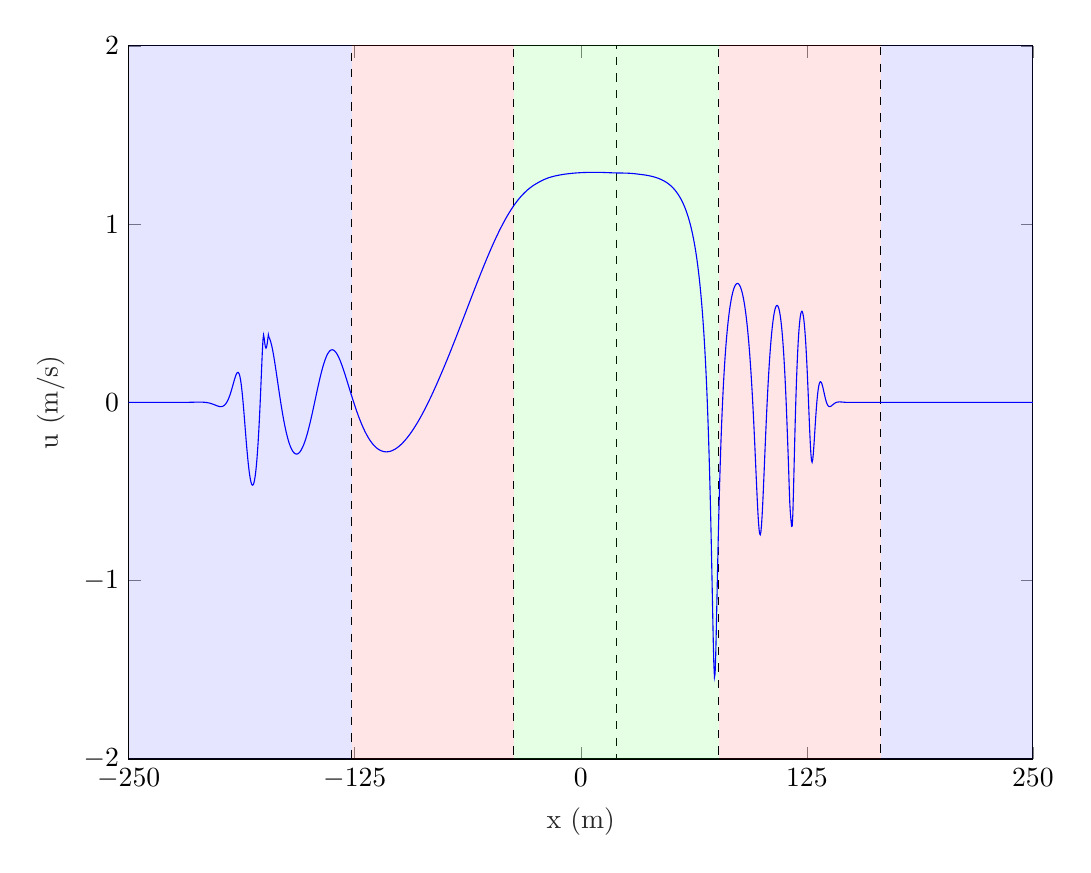
\begin{tikzpicture}

\begin{axis}[%
width=4.521in,
height=3.566in,
at={(0.758in,0.481in)},
scale only axis,
xmin=-250,
xmax=250,
xtick={-250, -125,    0,  125,  250},
xlabel style={font=\color{white!15!black}},
xlabel={x (m)},
ymin=-2,
ymax=2,
ytick={-2, -1,  0,  1,  2},
ylabel style={font=\color{white!15!black}},
ylabel={u (m/s)},
axis background/.style={fill=white}
]

\addplot[area legend, dashed, draw=black, fill=blue, fill opacity=0.1, forget plot]
table[row sep=crcr] {%
x	y\\
-250	-3\\
-250	3\\
-126.679671409596	3\\
-126.679671409596	-3\\
}--cycle;

\addplot[area legend, draw=none, fill=red, fill opacity=0.1, forget plot]
table[row sep=crcr] {%
x	y\\
-126.679671409596	-3\\
-126.679671409596	3\\
-37.0611924008642	3\\
-37.0611924008642	-3\\
}--cycle;

\addplot[area legend, dashed, draw=black, fill=green, fill opacity=0.1, forget plot]
table[row sep=crcr] {%
x	y\\
-37.0611924008642	-3\\
-37.0611924008642	3\\
19.5880540963537	3\\
19.5880540963537	-3\\
}--cycle;

\addplot[area legend, draw=none, fill=green, fill opacity=0.1, forget plot]
table[row sep=crcr] {%
x	y\\
19.5880540963537	-3\\
19.5880540963537	3\\
76.2373005935716	3\\
76.2373005935716	-3\\
}--cycle;

\addplot[area legend, dashed, draw=black, fill=red, fill opacity=0.1, forget plot]
table[row sep=crcr] {%
x	y\\
76.2373005935716	-3\\
76.2373005935716	3\\
165.855779602303	3\\
165.855779602303	-3\\
}--cycle;

\addplot[area legend, draw=none, fill=blue, fill opacity=0.1, forget plot]
table[row sep=crcr] {%
x	y\\
165.855779602303	-3\\
165.855779602303	3\\
250	3\\
250	-3\\
}--cycle;
\addplot [color=blue, forget plot]
  table[row sep=crcr]{%
-250.100003333444	0\\
-249.76665888863	6.13463393056353e-09\\
-249.433314443815	1.44388481475272e-08\\
-249.099969999	2.86360053770751e-08\\
-248.766625554185	4.82796270603448e-08\\
-248.43328110937	7.29633155957016e-08\\
-248.099936664555	1.0231445406227e-07\\
-247.766592219741	1.35988331504785e-07\\
-247.433247774926	1.7366134099767e-07\\
-247.099903330111	2.15024520212177e-07\\
-246.766558885296	2.59776689339051e-07\\
-246.433214440481	3.07617256144819e-07\\
-246.099869995667	3.58239188083399e-07\\
-245.766525550852	4.11321049625667e-07\\
-245.433181106037	4.66519252996788e-07\\
-245.099836661222	5.23459728138202e-07\\
-244.766492216407	5.81729045283642e-07\\
-244.433147771592	6.40865807528679e-07\\
-244.099803326778	7.003504820526e-07\\
-243.766458881963	7.59596320050128e-07\\
-243.433114437148	8.17938922469391e-07\\
-243.099769992333	8.74625386263556e-07\\
-242.766425547518	9.28800690871169e-07\\
-242.433081102703	9.79514315901907e-07\\
-242.099736657889	1.02567044625707e-06\\
-241.766392213074	1.06605057608351e-06\\
-241.433047768259	1.09928774203663e-06\\
-241.099703323444	1.1238557915187e-06\\
-240.766358878629	1.13805715911681e-06\\
-240.433014433814	1.14001015165147e-06\\
-240.099669989	1.12763714952503e-06\\
-239.766325544185	1.0986524175107e-06\\
-239.43298109937	1.05055116975084e-06\\
-239.099636654555	9.80599386708388e-07\\
-238.76629220974	8.8582436777154e-07\\
-238.432947764926	7.63006704510624e-07\\
-238.099603320111	6.0867468758521e-07\\
-237.766258875296	4.19099397253833e-07\\
-237.432914430481	1.90294398358133e-07\\
-237.099569985666	-8.19830636634186e-08\\
-236.766225540851	-4.02227482760647e-07\\
-236.432881096037	-7.75174482943554e-07\\
-236.099536651222	-1.20578717130706e-06\\
-235.766192206407	-1.699236097943e-06\\
-235.432847761592	-2.26087304474552e-06\\
-235.099503316777	-2.89619790784034e-06\\
-234.766158871962	-3.6108167499982e-06\\
-234.432814427148	-4.4103909086248e-06\\
-234.099469982333	-5.30057772314618e-06\\
-233.766125537518	-6.28695711713049e-06\\
-233.432781092703	-7.37494881904661e-06\\
-233.099436647888	-8.56971366283604e-06\\
-232.766092203073	-9.87604261364799e-06\\
-232.432747758259	-1.12982275398064e-05\\
-232.099403313444	-1.28399169401407e-05\\
-231.766058868629	-1.4503950742971e-05\\
-231.432714423814	-1.62921870155107e-05\\
-231.099369978999	-1.82052715284121e-05\\
-230.766025534184	-2.02424341441377e-05\\
-230.43268108937	-2.24012438502586e-05\\
-230.099336644555	-2.46773189685972e-05\\
-229.76599219974	-2.70640362950192e-05\\
-229.432647754925	-2.95522107912859e-05\\
-229.09930331011	-3.21297427785008e-05\\
-228.765958865296	-3.47812488544543e-05\\
-228.432614420481	-3.74876584556463e-05\\
-228.099269975666	-4.0225795727713e-05\\
-227.765925530851	-4.2967931840349e-05\\
-227.432581086036	-4.56813236635478e-05\\
-227.099236641221	-4.83277243192551e-05\\
-226.765892196407	-5.0862890360138e-05\\
-226.432547751592	-5.32360733395727e-05\\
-226.099203306777	-5.53892192852153e-05\\
-225.765858861962	-5.72583203159055e-05\\
-225.432514417147	-5.8768941199259e-05\\
-225.099169972332	-5.98394724830536e-05\\
-224.765825527518	-6.03791361524394e-05\\
-224.432481082703	-6.02877912052027e-05\\
-224.099136637888	-5.94555545276234e-05\\
-223.765792193073	-5.77625862612249e-05\\
-223.432447748258	-5.50787900806399e-05\\
-223.099103303443	-5.12638214270079e-05\\
-222.765758858629	-4.61670875649387e-05\\
-222.432414413814	-3.96279579939492e-05\\
-222.099069968999	-3.14761384716251e-05\\
-221.765725524184	-2.15322761727112e-05\\
-221.432381079369	-9.60877755361762e-06\\
-221.099036634554	4.48907098834909e-06\\
-220.76569218974	2.09617043242388e-05\\
-220.432347744925	4.00135035247006e-05\\
-220.09900330011	6.18506568605191e-05\\
-219.765658855295	8.66785681871711e-05\\
-219.43231441048	0.000114698850667266\\
-219.098969965666	0.000146105748183863\\
-218.765625520851	0.000181081926845586\\
-218.432281076036	0.000219794016312289\\
-218.098936631221	0.000262387055339592\\
-217.765592186406	0.000308978587143755\\
-217.432247741591	0.000359651932019649\\
-217.098903296777	0.00041444877739019\\
-216.765558851962	0.000473360757413998\\
-216.432214407147	0.000536320836756535\\
-216.098869962332	0.000603193363887234\\
-215.765525517517	0.000673763577100946\\
-215.432181072702	0.000747726398928257\\
-215.098836627888	0.000824674490795059\\
-214.765492183073	0.000904085686597001\\
-214.432147738258	0.000985309902664627\\
-214.098803293443	0.00106755562413412\\
-213.765458848628	0.0011498759855719\\
-213.432114403813	0.00123115493463584\\
-213.098769958999	0.00131009335504623\\
-212.765425514184	0.00138519569001001\\
-212.432081069369	0.00145475690319415\\
-212.098736624554	0.00151685172373675\\
-211.765392179739	0.00156933610264009\\
-211.432047734924	0.00160978884235261\\
-211.09870329011	0.00163559907267297\\
-210.765358845295	0.00164385739379364\\
-210.43201440048	0.00163142449120048\\
-210.098669955665	0.00159491791896971\\
-209.76532551085	0.00153072293006365\\
-209.431981066036	0.00143500789668412\\
-209.098636621221	0.00130374694551816\\
-208.765292176406	0.0011327518651327\\
-208.431947731591	0.000917710481073234\\
-208.098603286776	0.000654237673897488\\
-207.765258841961	0.000337933561995472\\
-207.431914397147	-3.55459810719597e-05\\
-207.098569952332	-0.000470404312387269\\
-206.765225507517	-0.000970604424780672\\
-206.431881062702	-0.00153976373112746\\
-206.098536617887	-0.00218102980701314\\
-205.765192173072	-0.00289693619798138\\
-205.431847728258	-0.00368924623300358\\
-205.098503283443	-0.00455879326868194\\
-204.765158838628	-0.00550529568003214\\
-204.431814393813	-0.00652716470392008\\
-204.098469948998	-0.00762130161262401\\
-203.765125504183	-0.00878288818913194\\
-203.431781059369	-0.0100051701076874\\
-203.098436614554	-0.0112792420912415\\
-202.765092169739	-0.0125938340643414\\
-202.431747724924	-0.0139351036300062\\
-202.098403280109	-0.0152864488124637\\
-201.765058835294	-0.0166283321215872\\
-201.43171439048	-0.0179381288188484\\
-201.098369945665	-0.0191900204316971\\
-200.76502550085	-0.0203549375658341\\
-200.431681056035	-0.0214004981106055\\
-200.09833661122	-0.0222910584256694\\
-199.764992166406	-0.0229876012464607\\
-199.431647721591	-0.0234491881582524\\
-199.098303276776	-0.0236305057392463\\
-198.764958831961	-0.0234845896050819\\
-198.431614387146	-0.0229623699782244\\
-198.098269942331	-0.0220132616483836\\
-197.764925497517	-0.0205857876500526\\
-197.431581052702	-0.0186283192212179\\
-197.098236607887	-0.0160899348114528\\
-196.764892163072	-0.0129214160760906\\
-196.431547718257	-0.00907639739623862\\
-196.098203273442	-0.00451266395988684\\
-195.764858828628	0.00080637179260943\\
-195.431514383813	0.00690993046055584\\
-195.098169938998	0.0138179773412283\\
-194.764825494183	0.0215391090967959\\
-194.431481049368	0.0300680066534385\\
-194.098136604553	0.0393827096923018\\
-193.764792159739	0.0494414673052402\\
-193.431447714924	0.0601792214838995\\
-193.098103270109	0.0715036864884404\\
-192.764758825294	0.0832910278379426\\
-192.431414380479	0.0953811839022342\\
-192.098069935665	0.107572938457956\\
-191.76472549085	0.119618873471346\\
-191.431381046035	0.131220904238809\\
-191.09803660122	0.142026015051598\\
-190.764692156405	0.151624398341005\\
-190.43134771159	0.159550015683423\\
-190.098003266776	0.165285736385491\\
-189.764658821961	0.168274444545239\\
-189.431314377146	0.167943402669332\\
-189.097969932331	0.163725871268641\\
-188.764625487516	0.155110399089423\\
-188.431281042701	0.141689927251056\\
-188.097936597887	0.123216486698993\\
-187.764592153072	0.0996498540027459\\
-187.431247708257	0.0711899856183547\\
-187.097903263442	0.0382818524268052\\
-186.764558818627	0.00158947474048017\\
-186.431214373812	-0.038056664775388\\
-186.097869928998	-0.0797270698590846\\
-185.764525484183	-0.122461833500876\\
-185.431181039368	-0.165328585574071\\
-185.097836594553	-0.207463247853734\\
-184.764492149738	-0.248093752153355\\
-184.431147704923	-0.28654880789866\\
-184.097803260109	-0.322255837201127\\
-183.764458815294	-0.354732578908991\\
-183.431114370479	-0.38357518763631\\
-183.097769925664	-0.408445258386797\\
-182.764425480849	-0.429057437556606\\
-182.431081036035	-0.445167599470215\\
-182.09773659122	-0.456562937476088\\
-181.764392146405	-0.463053184304175\\
-181.43104770159	-0.464461656293392\\
-181.097703256775	-0.460624246847059\\
-180.76435881196	-0.451381482435483\\
-180.431014367146	-0.436575164762875\\
-180.097669922331	-0.416047192848518\\
-179.764325477516	-0.389639297008228\\
-179.430981032701	-0.357194761088273\\
-179.097636587886	-0.318563121409709\\
-178.764292143071	-0.273609373082813\\
-178.430947698257	-0.222230153409006\\
-178.097603253442	-0.164381128593939\\
-177.764258808627	-0.100124351820906\\
-177.430914363812	-0.0297120647500389\\
-177.097569918997	0.0462586215119698\\
-176.764225474182	0.126541483092862\\
-176.430881029368	0.208592857985577\\
-176.097536584553	0.287079906158463\\
-175.764192139738	0.350470133418277\\
-175.430847694923	0.377787263195449\\
-175.097503250108	0.360713403831326\\
-174.764158805294	0.331812432280356\\
-174.430814360479	0.311581940109211\\
-174.097469915664	0.304337590851951\\
-173.764125470849	0.31029550699836\\
-173.430781026034	0.328436476083111\\
-173.097436581219	0.355772001658608\\
-172.764092136405	0.379578948756514\\
-172.43074769159	0.36367542815721\\
-172.097403246775	0.359881272487503\\
-171.76405880196	0.348621204183206\\
-171.430714357145	0.338191066754006\\
-171.09736991233	0.32559899957733\\
-170.764025467516	0.310924487678638\\
-170.430681022701	0.294458798352342\\
-170.097336577886	0.276419064312091\\
-169.763992133071	0.257021132740457\\
-169.430647688256	0.236479655119529\\
-169.097303243441	0.215007698984846\\
-168.763958798627	0.192814007791429\\
-168.430614353812	0.170098279261579\\
-168.097269908997	0.14704481637532\\
-167.763925464182	0.123824521552474\\
-167.430581019367	0.100591329888104\\
-167.097236574552	0.0774824548929832\\
-166.763892129738	0.0546217742186814\\
-166.430547684923	0.0321180796576593\\
-166.097203240108	0.010063943353559\\
-165.763858795293	-0.0114607861138595\\
-165.430514350478	-0.0323889347396202\\
-165.097169905664	-0.0526669984484571\\
-164.763825460849	-0.0722596502214893\\
-164.430481016034	-0.0911214282954009\\
-164.097136571219	-0.109192947941059\\
-163.763792126404	-0.126447773883268\\
-163.430447681589	-0.142864601599799\\
-163.097103236775	-0.158426688870401\\
-162.76375879196	-0.173122481353256\\
-162.430414347145	-0.186941531738222\\
-162.09706990233	-0.199876446427296\\
-161.763725457515	-0.211925155372295\\
-161.4303810127	-0.223089137088655\\
-161.097036567886	-0.233369025196209\\
-160.763692123071	-0.242766969578029\\
-160.430347678256	-0.251285261323119\\
-160.097003233441	-0.25892926399911\\
-159.763658788626	-0.2657048216895\\
-159.430314343811	-0.271620705812722\\
-159.096969898997	-0.276684793219508\\
-158.763625454182	-0.280905666893413\\
-158.430281009367	-0.284291613131735\\
-158.096936564552	-0.286852980653416\\
-157.763592119737	-0.288598884147515\\
-157.430247674922	-0.289538414570958\\
-157.096903230108	-0.289680574673503\\
-156.763558785293	-0.289037982684004\\
-156.430214340478	-0.287618728560914\\
-156.096869895663	-0.285434321849007\\
-155.763525450848	-0.282495728920039\\
-155.430181006034	-0.278814692748659\\
-155.096836561219	-0.2744032689931\\
-154.763492116404	-0.269273700140062\\
-154.430147671589	-0.263439540757642\\
-154.096803226774	-0.2569142831714\\
-153.763458781959	-0.249712615512594\\
-153.430114337145	-0.241849555458705\\
-153.09676989233	-0.233340068090049\\
-152.763425447515	-0.224199951935964\\
-152.4300810027	-0.214446177414812\\
-152.096736557885	-0.204096806777063\\
-151.76339211307	-0.193172850129951\\
-151.430047668256	-0.181697640309158\\
-151.096703223441	-0.169693602653904\\
-150.763358778626	-0.157182881404304\\
-150.430014333811	-0.144188311880065\\
-150.096669888996	-0.130733132835925\\
-149.763325444181	-0.116836675200687\\
-149.429980999367	-0.10253158816289\\
-149.096636554552	-0.0878697576258514\\
-148.763292109737	-0.0728924391605877\\
-148.429947664922	-0.0576434656667303\\
-148.096603220107	-0.0421708991724228\\
-147.763258775293	-0.0265273610871317\\
-147.429914330478	-0.0107682624631585\\
-147.096569885663	0.00505168670999148\\
-146.763225440848	0.0208816074449786\\
-146.429880996033	0.0366749078236233\\
-146.096536551218	0.0523881765461724\\
-145.763192106404	0.0679798253341316\\
-145.429847661589	0.0834059562877814\\
-145.096503216774	0.0986096955713785\\
-144.763158771959	0.113531974340032\\
-144.429814327144	0.128136410231251\\
-144.096469882329	0.142389338510297\\
-143.763125437515	0.156242853028726\\
-143.4297809927	0.169651239291506\\
-143.096436547885	0.182569388830603\\
-142.76309210307	0.1949559572602\\
-142.429747658255	0.206765993975674\\
-142.09640321344	0.217961827005221\\
-141.763058768626	0.228502547119028\\
-141.429714323811	0.238347828843456\\
-141.096369878996	0.247453388523923\\
-140.763025434181	0.25578353010203\\
-140.429680989366	0.263321982977603\\
-140.096336544551	0.270068972846635\\
-139.762992099737	0.276030002921574\\
-139.429647654922	0.281197846363478\\
-139.096303210107	0.28555508758356\\
-138.762958765292	0.289098065461618\\
-138.429614320477	0.291829606824143\\
-138.096269875663	0.293757203101085\\
-137.762925430848	0.29487482389701\\
-137.429580986033	0.295155156449462\\
-137.096236541218	0.294589706432979\\
-136.762892096403	0.293213316426059\\
-136.429547651588	0.291103032971138\\
-136.096203206774	0.288299368239492\\
-135.762858761959	0.284790874583886\\
-135.429514317144	0.280608171346814\\
-135.096169872329	0.275773482818684\\
-134.762825427514	0.270313377214623\\
-134.429480982699	0.264262208294958\\
-134.096136537885	0.257652223655382\\
-133.76279209307	0.250515902155014\\
-133.429447648255	0.242889733267544\\
-133.09610320344	0.234809415910158\\
-132.762758758625	0.22630903519255\\
-132.42941431381	0.217424897060003\\
-132.096069868996	0.20819211073697\\
-131.762725424181	0.198647206875946\\
-131.429380979366	0.188823497592163\\
-131.096036534551	0.178753811222527\\
-130.762692089736	0.168470433391792\\
-130.429347644921	0.158004500845176\\
-130.096003200107	0.147385080607345\\
-129.762658755292	0.136639726833823\\
-129.429314310477	0.125794442766628\\
-129.095969865662	0.114875610179264\\
-128.762625420847	0.10390404276778\\
-128.429280976033	0.0929018208152523\\
-128.095936531218	0.0818952831961339\\
-127.762592086403	0.0709032499501106\\
-127.429247641588	0.0599411826185629\\
-127.095903196773	0.0490301895363074\\
-126.762558751958	0.0381883147766996\\
-126.429214307144	0.0274337774963311\\
-126.095869862329	0.0167784311741007\\
-125.762525417514	0.00623143345447912\\
-125.429180972699	-0.00419037811649531\\
-125.095836527884	-0.0144739872776134\\
-124.762492083069	-0.0246132319464261\\
-124.429147638255	-0.0345969031768424\\
-124.09580319344	-0.0444154393469815\\
-123.762458748625	-0.0540626917591715\\
-123.42911430381	-0.0635306855284379\\
-123.095769858995	-0.0728131317435517\\
-122.76242541418	-0.081905140198033\\
-122.429080969366	-0.0908008344317977\\
-122.095736524551	-0.0994965881241766\\
-121.762392079736	-0.107988125003678\\
-121.429047634921	-0.116272558794375\\
-121.095703190106	-0.124346620315546\\
-120.762358745291	-0.132208301390806\\
-120.429014300477	-0.13985557880608\\
-120.095669855662	-0.147287171937452\\
-119.762325410847	-0.154501731787035\\
-119.428980966032	-0.16149864402277\\
-119.095636521217	-0.168277315086315\\
-118.762292076403	-0.174837424259112\\
-118.428947631588	-0.181178935178789\\
-118.095603186773	-0.187302668043715\\
-117.762258741958	-0.193209290482258\\
-117.428914297143	-0.198899334921954\\
-117.095569852328	-0.204374018050019\\
-116.762225407514	-0.209634461453993\\
-116.428880962699	-0.214681539143704\\
-116.095536517884	-0.219515928337773\\
-115.762192073069	-0.224140266081289\\
-115.428847628254	-0.228556183774535\\
-115.095503183439	-0.232764870009631\\
-114.762158738625	-0.236768170200443\\
-114.42881429381	-0.24056828162798\\
-114.095469848995	-0.244167087145199\\
-113.76212540418	-0.247566192871391\\
-113.428780959365	-0.250767942860585\\
-113.09543651455	-0.253774678170553\\
-112.762092069736	-0.256588392097439\\
-112.428747624921	-0.259211445135719\\
-112.095403180106	-0.261645918964444\\
-111.762058735291	-0.263893830514834\\
-111.428714290476	-0.265957858856098\\
-111.095369845662	-0.267840259312671\\
-110.762025400847	-0.269543183260678\\
-110.428680956032	-0.271068807012613\\
-110.095336511217	-0.27241953435641\\
-109.761992066402	-0.273597537142411\\
-109.428647621587	-0.274605348622949\\
-109.095303176773	-0.275445202189224\\
-108.761958731958	-0.27611916111817\\
-108.428614287143	-0.27662961813254\\
-108.095269842328	-0.276978883174646\\
-107.761925397513	-0.277169136549517\\
-107.428580952698	-0.277202726931342\\
-107.095236507884	-0.277081594997214\\
-106.761892063069	-0.276807891332943\\
-106.428547618254	-0.276383912910185\\
-106.095203173439	-0.275811749115246\\
-105.761858728624	-0.275093327874779\\
-105.428514283809	-0.27423075597119\\
-105.095169838995	-0.273226013120295\\
-104.76182539418	-0.272081216078598\\
-104.428480949365	-0.270798183308677\\
-104.09513650455	-0.269378876581033\\
-103.761792059735	-0.267825286889697\\
-103.42844761492	-0.266139193719331\\
-103.095103170106	-0.264322753016319\\
-102.761758725291	-0.262377833216804\\
-102.428414280476	-0.260306708617715\\
-102.095069835661	-0.258111146459488\\
-101.761725390846	-0.255792884729729\\
-101.428380946032	-0.253353284919404\\
-101.095036501217	-0.250794086315615\\
-100.761692056402	-0.248116970289671\\
-100.428347611587	-0.245323888415205\\
-100.095003166772	-0.242416131821447\\
-99.7616587219574	-0.239395389218123\\
-99.4283142771426	-0.236263377858745\\
-99.0949698323277	-0.233021575729135\\
-98.7616253875129	-0.229671634795004\\
-98.4282809426981	-0.226215459329983\\
-98.0949364978833	-0.222652813665967\\
-97.7615920530684	-0.21899091779159\\
-97.4282476082536	-0.215233538982991\\
-97.0949031634388	-0.211375415442754\\
-96.7615587186239	-0.207411357533966\\
-96.4282142738091	-0.203346016020097\\
-96.0948698289943	-0.199181654131131\\
-95.7615253841795	-0.194919802933619\\
-95.4281809393646	-0.190561480906897\\
-95.0948364945498	-0.186110604732938\\
-94.761492049735	-0.181569925457946\\
-94.4281476049202	-0.176935627328535\\
-94.0948031601053	-0.172215181800811\\
-93.7614587152905	-0.16740966128698\\
-93.4281142704757	-0.162513819342679\\
-93.0947698256608	-0.157536282411802\\
-92.761425380846	-0.15248191239325\\
-92.4280809360312	-0.147344035425046\\
-92.0947364912164	-0.142119936646186\\
-91.7613920464015	-0.136816664896967\\
-91.4280476015867	-0.131444394108829\\
-91.0947031567719	-0.126009183017894\\
-90.7613587119571	-0.120504905269996\\
-90.4280142671422	-0.114918607210218\\
-90.0946698223274	-0.109245602979578\\
-89.7613253775126	-0.103506986182326\\
-89.4279809326977	-0.0976839282205722\\
-89.0946364878829	-0.091757977244239\\
-88.7612920430681	-0.0857306513125577\\
-88.4279475982533	-0.079613142675556\\
-88.0946031534384	-0.073417060431511\\
-87.7612587086236	-0.0671471472351747\\
-87.4279142638088	-0.0608108871762026\\
-87.094569818994	-0.0544078571533463\\
-86.7612253741791	-0.0479492609197943\\
-86.4278809293643	-0.0414354258645655\\
-86.0945364845495	-0.0348496281221864\\
-85.7611920397347	-0.0282060095260693\\
-85.4278475949198	-0.0215097119808289\\
-85.094503150105	-0.01475491601417\\
-84.7611587052902	-0.00794652380071578\\
-84.4278142604753	-0.0010873941349137\\
-84.0944698156605	0.00582444284609525\\
-83.7611253708457	0.0127972230067257\\
-83.4277809260309	0.0198391970772832\\
-83.094436481216	0.0269442392827899\\
-82.7610920364012	0.0341063412243054\\
-82.4277475915864	0.0413243641443475\\
-82.0944031467716	0.0485970924530545\\
-81.7610587019567	0.0559228305156551\\
-81.4277142571419	0.0632959991916561\\
-81.0943698123271	0.0707101147457519\\
-80.7610253675122	0.0781595290965652\\
-80.4276809226974	0.0856397031915796\\
-80.0943364778826	0.093171068354366\\
-79.7609920330678	0.100758647686774\\
-79.4276475882529	0.108401899090842\\
-79.0943031434381	0.116096086724584\\
-78.7609586986233	0.123837121102384\\
-78.4276142538084	0.131622074404295\\
-78.0942698089936	0.139445586546025\\
-77.7609253641788	0.147305197372379\\
-77.4275809193639	0.155201735482566\\
-77.0942364745491	0.163129651046492\\
-76.7608920297343	0.171087413369193\\
-76.4275475849195	0.179075881763349\\
-76.0942031401046	0.187091783491728\\
-75.7608586952898	0.195135840575202\\
-75.427514250475	0.203208321775781\\
-75.0941698056602	0.211308872244616\\
-74.7608253608453	0.219437844373231\\
-74.4274809160305	0.227598336196796\\
-74.0941364712157	0.235792308005268\\
-73.7607920264008	0.24402108463801\\
-73.427447581586	0.252287827836454\\
-73.0941031367712	0.260595582958088\\
-72.7607586919564	0.268946652874844\\
-72.4274142471415	0.277343366249995\\
-72.0940698023267	0.285786051250807\\
-71.7607253575119	0.294272742984654\\
-71.4273809126971	0.302799124753211\\
-71.0940364678822	0.31135589721911\\
-70.7606920230674	0.319930391847591\\
-70.4273475782526	0.328510727055962\\
-70.0940031334378	0.337086131836925\\
-69.7606586886229	0.345645254193838\\
-69.4273142438081	0.354184866029696\\
-69.0939697989933	0.362725753623334\\
-68.7606253541784	0.371311415092541\\
-68.4272809093636	0.379978153402164\\
-68.0939364645488	0.388704157843507\\
-67.760592019734	0.397441249670836\\
-67.4272475749191	0.406200461884421\\
-67.0939031301043	0.414976558465495\\
-66.7605586852895	0.423754112398371\\
-66.4272142404747	0.432549036414426\\
-66.0938697956598	0.441347378907679\\
-65.760525350845	0.450145777289246\\
-65.4271809060302	0.458939251415563\\
-65.0938364612153	0.467728219879463\\
-64.7604920164005	0.476514964436514\\
-64.4271475715857	0.485306316079262\\
-64.0938031267709	0.494111337799249\\
-63.760458681956	0.502933812809382\\
-63.4271142371412	0.51176414260205\\
-63.0937697923264	0.520587341344786\\
-62.7604253475116	0.529396331866342\\
-62.4270809026967	0.53820037932725\\
-62.0937364578819	0.547015550637712\\
-61.7603920130671	0.555834095485057\\
-61.4270475682522	0.564639977203683\\
-61.0937031234374	0.57343867867342\\
-60.7603586786226	0.582224961244681\\
-60.4270142338078	0.590997518746364\\
-60.0936697889929	0.599757391078811\\
-59.7603253441781	0.608503887423618\\
-59.4269808993633	0.617236870514004\\
-59.0936364545485	0.625955714695144\\
-58.7602920097336	0.63465727297172\\
-58.4269475649188	0.643339071109204\\
-58.093603120104	0.652001275018693\\
-57.7602586752892	0.660645510302235\\
-57.4269142304743	0.6692693309108\\
-57.0935697856595	0.6778715820769\\
-56.7602253408447	0.686450378039073\\
-56.4268808960298	0.695003986545688\\
-56.093536451215	0.703531541299903\\
-55.7601920064002	0.71203329616454\\
-55.4268475615854	0.720508858317404\\
-55.0935031167705	0.728956298417748\\
-54.7601586719557	0.737374513331703\\
-54.4268142271409	0.745761837665744\\
-54.0934697823261	0.754116536137173\\
-53.7601253375112	0.762437674359648\\
-53.4267808926964	0.770724512360036\\
-53.0934364478816	0.778975673618923\\
-52.7600920030667	0.787188591701368\\
-52.4267475582519	0.795363201158622\\
-52.0934031134371	0.803495255409413\\
-51.7600586686223	0.811586344553016\\
-51.4267142238074	0.819630759537003\\
-51.0933697789926	0.827631493048922\\
-50.7600253341778	0.835582626939327\\
-50.426680889363	0.843487316326691\\
-50.0933364445481	0.85134156250961\\
-49.7599919997333	0.859146725278247\\
-49.4266475549185	0.866899597146069\\
-49.0933031101036	0.874597161397003\\
-48.7599586652888	0.882233266134548\\
-48.426614220474	0.889804370448326\\
-48.0932697756592	0.897308666111769\\
-47.7599253308443	0.904742203805174\\
-47.4265808860295	0.912106371783462\\
-47.0932364412147	0.919400663107802\\
-46.7598919963999	0.926623177004098\\
-46.426547551585	0.933778845909822\\
-46.0932031067702	0.94086513324635\\
-45.7598586619554	0.947883975848277\\
-45.4265142171406	0.954830072741172\\
-45.0931697723257	0.961698482626361\\
-44.7598253275109	0.968494482573636\\
-44.4264808826961	0.975214305970044\\
-44.0931364378812	0.981861091160336\\
-43.7597919930664	0.988435879231857\\
-43.4264475482516	0.994939457736065\\
-43.0931031034368	1.00136979595879\\
-42.7597586586219	1.00772575213883\\
-42.4264142138071	1.01400601172173\\
-42.0930697689923	1.0202071435054\\
-41.7597253241775	1.0263285388999\\
-41.4263808793626	1.03236827627505\\
-41.0930364345478	1.03832466941183\\
-40.759691989733	1.04419723823782\\
-40.4263475449181	1.04998381579529\\
-40.0930031001033	1.05568405844097\\
-39.7596586552885	1.06129823441859\\
-39.4263142104737	1.06682477429117\\
-39.0929697656588	1.07226244025689\\
-38.759625320844	1.07761193927645\\
-38.4262808760292	1.0828734476884\\
-38.0929364312144	1.08804578100176\\
-37.7595919863995	1.09312867579392\\
-37.4262475415847	1.09812216828153\\
-37.0929030967699	1.10302609813086\\
-36.759558651955	1.10784026442299\\
-36.4262142071402	1.11256531432541\\
-36.0928697623254	1.11720162454138\\
-35.7595253175106	1.12174840818724\\
-35.4261808726957	1.12620625289314\\
-35.0928364278809	1.13057554224513\\
-34.7594919830661	1.13485622742923\\
-34.4261475382513	1.13904838876255\\
-34.0928030934364	1.1431523377378\\
-33.7594586486216	1.14716543989753\\
-33.4261142038068	1.15108793284238\\
-33.0927697589919	1.15492516262812\\
-32.7594253141771	1.15867670547249\\
-32.4260808693623	1.16234808109726\\
-32.0927364245475	1.16594256188457\\
-31.7593919797326	1.16945813439129\\
-31.4260475349178	1.17289941256632\\
-31.092703090103	1.17626449771383\\
-30.7593586452882	1.17955298547338\\
-30.4260142004733	1.1827637249779\\
-30.0926697556585	1.18589793262593\\
-29.7593253108437	1.18895412181169\\
-29.4259808660289	1.19193298030537\\
-29.092636421214	1.19483117408499\\
-28.7592919763992	1.19764210411701\\
-28.4259475315844	1.20037644817982\\
-28.0926030867695	1.2030480541531\\
-27.7592586419547	1.20566033461795\\
-27.4259141971399	1.20821575670852\\
-27.0925697523251	1.21071586210604\\
-26.7592253075102	1.21314620812941\\
-26.4258808626954	1.21546808384413\\
-26.0925364178806	1.21767938440222\\
-25.7591919730658	1.21980315001525\\
-25.4258475282509	1.22186813783002\\
-25.0925030834361	1.22389840955624\\
-24.7591586386213	1.22590763876624\\
-24.4258141938064	1.22789436255762\\
-24.0924697489916	1.22986111913653\\
-23.7591253041768	1.23181003350661\\
-23.425780859362	1.2337254135217\\
-23.0924364145471	1.23561895043975\\
-22.7590919697323	1.23747257037691\\
-22.4257475249175	1.23929617892172\\
-22.0924030801027	1.24107500006213\\
-21.7590586352878	1.24281378102036\\
-21.425714190473	1.2445107817533\\
-21.0923697456582	1.2461557211238\\
-20.7590253008433	1.24775544139077\\
-20.4256808560285	1.24930812434029\\
-20.0923364112137	1.25080629996228\\
-19.7589919663989	1.25225602308648\\
-19.425647521584	1.25365761789356\\
-19.0923030767692	1.2550095835148\\
-18.7589586319544	1.25630993940723\\
-18.4256141871396	1.25756432474565\\
-18.0922697423247	1.25877295499548\\
-17.7589252975099	1.25993570815665\\
-17.4255808526951	1.26105189261924\\
-17.0922364078803	1.26212686099165\\
-16.7588919630654	1.26316583653393\\
-16.4255475182506	1.26416963687801\\
-16.0922030734358	1.26513796876537\\
-15.7588586286209	1.2660737015337\\
-15.4255141838061	1.26698145817827\\
-15.0921697389913	1.2678628136262\\
-14.7588252941765	1.26871280446918\\
-14.4254808493616	1.26952640814992\\
-14.0921364045468	1.27030814975646\\
-13.758791959732	1.27106897491046\\
-13.4254475149172	1.27180929795533\\
-13.0921030701023	1.27252648311029\\
-12.7587586252875	1.27321982701384\\
-12.4254141804727	1.27388893109039\\
-12.0920697356578	1.27453910108161\\
-11.758725290843	1.27517291698583\\
-11.4253808460282	1.27578871483189\\
-11.0920364012134	1.27638700133955\\
-10.7586919563985	1.27696793986177\\
-10.4253475115837	1.27753320614233\\
-10.0920030667689	1.27808349858927\\
-9.75865862195403	1.27861674868567\\
-9.4253141771392	1.2791324749348\\
-9.09196973232437	1.27963150883703\\
-8.75862528750955	1.28011508230276\\
-8.42528084269472	1.28058559852945\\
-8.09193639787989	1.28104317557571\\
-7.75859195306506	1.28148716252861\\
-7.42524750825024	1.28191673046896\\
-7.09190306343541	1.28233134298854\\
-6.75855861862058	1.28273409296847\\
-6.42521417380576	1.28312941939884\\
-6.09186972899093	1.28351304265785\\
-5.7585252841761	1.28388264629365\\
-5.42518083936127	1.28423889737105\\
-5.09183639454645	1.2845824920405\\
-4.75849194973162	1.28491525774766\\
-4.42514750491679	1.28523969911008\\
-4.09180306010197	1.28555277966746\\
-3.75845861528714	1.28585273625019\\
-3.42511417047231	1.28614040045522\\
-3.09176972565749	1.28641659486067\\
-2.75842528084266	1.28668478197121\\
-2.42508083602783	1.28694415170516\\
-2.091736391213	1.28719244009915\\
-1.75839194639818	1.2874293023366\\
-1.42504750158335	1.28765550912408\\
-1.09170305676852	1.28787173020924\\
-0.758358611953696	1.28807845951352\\
-0.425014167138869	1.28827705690771\\
-0.0916697223240419	1.28846620945902\\
0.241674722490785	1.28864583864115\\
0.575019167305612	1.28881600253125\\
0.908363612120439	1.28897653142356\\
1.24170805693527	1.28912748398673\\
1.57505250175009	1.28926944507921\\
1.90839694656492	1.28940345302451\\
2.24174139137975	1.28952899065437\\
2.57508583619457	1.28964498906269\\
2.9084302810094	1.28975064068737\\
3.24177472582423	1.28984669342844\\
3.57511917063906	1.28993353841757\\
3.90846361545388	1.29001193561759\\
4.24180806026871	1.29008092292103\\
4.57515250508354	1.29013847898314\\
4.90849694989836	1.29018467806208\\
5.24184139471319	1.29022321117735\\
5.57518583952802	1.29025965307968\\
5.90853028434285	1.2902884963488\\
6.24187472915764	1.29029638147823\\
6.57521917397247	1.29028688255952\\
6.9085636187873	1.2902756934728\\
7.24190806360212	1.29026865792554\\
7.57525250841695	1.29028798822067\\
7.90859695323178	1.29026966768493\\
8.24194139804661	1.29019267750084\\
8.57528584286143	1.29011074505664\\
8.90863028767626	1.29004955291196\\
9.24197473249109	1.29001564817179\\
9.57531917730591	1.29002003606773\\
9.90866362212074	1.29004331621038\\
10.2420080669356	1.2900487657896\\
10.5753525117504	1.29004004157283\\
10.9086969565652	1.29001071386037\\
11.24204140138	1.28995874246216\\
11.5753858461949	1.28988460363732\\
11.9087302910097	1.28979037363211\\
12.2420747358245	1.28968197077542\\
12.5754191806394	1.28956329648855\\
12.9087636254542	1.28943783404891\\
13.242108070269	1.28930738750827\\
13.5754525150838	1.28917316252188\\
13.9087969598987	1.28903681766382\\
14.2421414047135	1.28889655940283\\
14.5754858495283	1.28875445330436\\
14.9088302943431	1.28861153383012\\
15.242174739158	1.28846926510509\\
15.5755191839728	1.28833118387742\\
15.9088636287876	1.28820059684342\\
16.2422080736025	1.28807734550115\\
16.5755525184173	1.28794690097427\\
16.9088969632321	1.28780352359195\\
17.2422414080469	1.28765576278526\\
17.5755858528618	1.28750951040011\\
17.9089302976766	1.28737172787544\\
18.2422747424914	1.28725203872027\\
18.5756191873062	1.28715154679554\\
18.9089636321211	1.28706469405367\\
19.2423080769359	1.28698708530711\\
19.5756525217507	1.28691651030163\\
19.9089969665656	1.28682344542122\\
20.2423414113804	1.28670970389207\\
20.5756858561952	1.28659958502042\\
20.90903030101	1.28650809824619\\
21.2423747458249	1.28643360905039\\
21.5757191906397	1.28638482738033\\
21.9090636354545	1.28636707421286\\
22.2424080802693	1.28636653106858\\
22.5757525250842	1.28636410830024\\
22.909096969899	1.28635079070204\\
23.2424414147139	1.28632794895717\\
23.5757858595287	1.28629442328811\\
23.9091303043435	1.28624556587287\\
24.2424747491584	1.28617839941732\\
24.5758191939732	1.28609230452927\\
24.909163638788	1.28598734122611\\
25.2425080836028	1.28586490684153\\
25.5758525284177	1.28572585545989\\
25.9091969732325	1.28556979841078\\
26.2425414180473	1.28540043708412\\
26.5758858628622	1.28522211214427\\
26.909230307677	1.28503674004393\\
27.2425747524918	1.28484134269026\\
27.5759191973066	1.28463110862346\\
27.9092636421215	1.28440192929689\\
28.2426080869363	1.28415090974005\\
28.5759525317511	1.28387597516841\\
28.9092969765659	1.28357557450403\\
29.2426414213808	1.28324656709337\\
29.5759858661956	1.28289045706801\\
29.9093303110104	1.28250926372702\\
30.2426747558252	1.28210799990613\\
30.5760192006401	1.28169360759099\\
30.9093636454549	1.28127584547031\\
31.2427080902697	1.2808552683565\\
31.5760525350846	1.28042596778299\\
31.9093969798994	1.27999802404679\\
32.2427414247142	1.27958643888943\\
32.576085869529	1.27918491565608\\
32.9094303143439	1.27878207795119\\
33.2427747591587	1.27837853023118\\
33.5761192039735	1.27796716553763\\
33.9094636487883	1.2775403805706\\
34.2428080936032	1.27710149963049\\
34.576152538418	1.27664811652252\\
34.9094969832328	1.27617568836884\\
35.2428414280477	1.27568175852226\\
35.5761858728625	1.27517080843419\\
35.9095303176773	1.27464464351565\\
36.2428747624921	1.27409810119504\\
36.576219207307	1.27352409892942\\
36.9095636521218	1.27291863001392\\
37.2429080969366	1.27228130118817\\
37.5762525417514	1.27161192227235\\
37.9095969865663	1.2709001328111\\
38.2429414313811	1.27014321298122\\
38.5762858761959	1.26935896495599\\
38.9096303210108	1.26856248958253\\
39.2429747658256	1.2677775317054\\
39.5763192106404	1.2670060325211\\
39.9096636554552	1.26618532585297\\
40.2430081002701	1.2652948001523\\
40.5763525450849	1.26435325594433\\
40.9096969898997	1.26336999880298\\
41.2430414347145	1.26233892649059\\
41.5763858795294	1.26126043525205\\
41.9097303243442	1.26013794598833\\
42.243074769159	1.25897157640945\\
42.5764192139738	1.25776072208645\\
42.9097636587887	1.25649989820682\\
43.2431081036035	1.25518623040148\\
43.5764525484183	1.25382354093974\\
43.9097969932332	1.25240789953991\\
44.243141438048	1.25093600237091\\
44.5764858828628	1.24940462114608\\
44.9098303276776	1.24780915337403\\
45.2431747724925	1.24614325423539\\
45.5765192173073	1.24440290175864\\
45.9098636621221	1.2425860844681\\
46.2432081069369	1.2406916897597\\
46.5765525517518	1.23871834672528\\
46.9098969965666	1.2366627513032\\
47.2432414413814	1.23452075161372\\
47.5765858861963	1.23228791908114\\
47.9099303310111	1.22995835757752\\
48.2432747758259	1.22752759184406\\
48.5766192206407	1.22498915347386\\
48.9099636654556	1.22233652054041\\
49.2433081102704	1.21956430784227\\
49.5766525550852	1.21666791466818\\
49.9099969999	1.21364224408023\\
50.2433414447149	1.21048204891346\\
50.5766858895297	1.20718163471266\\
50.9100303343445	1.2037357998359\\
51.2433747791594	1.20013924533467\\
51.5767192239742	1.19638395939577\\
51.910063668789	1.19246234434289\\
52.2434081136038	1.18836908539179\\
52.5767525584187	1.18409891000944\\
52.9100970032335	1.17964567134548\\
53.2434414480483	1.17500263212938\\
53.5767858928631	1.17016195974059\\
53.910130337678	1.16511407210378\\
54.2434747824928	1.15984894766231\\
54.5768192273076	1.15435533864297\\
54.9101636721225	1.14862058751633\\
55.2435081169373	1.14263140945929\\
55.5768525617521	1.13637278868512\\
55.9101970065669	1.12982927757591\\
56.2435414513818	1.1229840641216\\
56.5768858961966	1.11581975461923\\
56.9102303410114	1.10831748192558\\
57.2435747858262	1.10045794684895\\
57.5769192306411	1.09222082604631\\
57.9102636754559	1.08358368350299\\
58.2436081202707	1.07452270368929\\
58.5769525650855	1.06501314538753\\
58.9102970099004	1.05502882910387\\
59.2436414547152	1.04454189240832\\
59.57698589953	1.03352235518349\\
59.9103303443449	1.02193794206837\\
60.2436747891597	1.00975319698271\\
60.5770192339745	0.996929033642325\\
60.9103636787893	0.983423267358797\\
61.2437081236042	0.969189504510464\\
61.577052568419	0.954179644603534\\
61.9103970132338	0.938339020157197\\
62.2437414580486	0.92160928572334\\
62.5770859028635	0.903930999490424\\
62.9104303476783	0.885240878076476\\
63.2437747924931	0.865468268805992\\
63.577119237308	0.844534043044331\\
63.9104636821228	0.822349902907385\\
64.2438081269376	0.798817603232507\\
64.5771525717524	0.77382853968545\\
64.9104970165673	0.747262048018705\\
65.2438414613821	0.718983179391659\\
65.5771859061969	0.688841092578268\\
65.9105303510117	0.656667065172174\\
66.2438747958266	0.62227214366961\\
66.5772192406414	0.585444271373494\\
66.9105636854562	0.545945017386039\\
67.2439081302711	0.503505415364475\\
67.5772525750859	0.457821493595448\\
67.9105970199007	0.408548275129852\\
68.2439414647155	0.355292866898354\\
68.5772859095304	0.297606301961167\\
68.9106303543452	0.234973437837449\\
69.24397479916	0.166803427594692\\
69.5773192439748	0.0924197781905181\\
69.9106636887897	0.0110510875507939\\
70.2440081336045	-0.0781765730716874\\
70.5773525784193	-0.1762408646414\\
70.9106970232341	-0.284209726489175\\
71.244041468049	-0.403195419563092\\
71.5773859128638	-0.534241170874845\\
71.9107303576786	-0.678079089121384\\
72.2440748024935	-0.834622205335911\\
72.5774192473083	-1.00194611843381\\
72.9107636921231	-1.17433759616449\\
73.2441081369379	-1.3389732930062\\
73.5774525817528	-1.4721176248384\\
73.9107970265676	-1.54113140295595\\
74.2441414713824	-1.52324897462804\\
74.5774859161972	-1.4271675553024\\
74.9108303610121	-1.28362255757366\\
75.2441748058269	-1.12126397028556\\
75.5775192506417	-0.957789723710583\\
75.9108636954566	-0.802050726353808\\
76.2442081402714	-0.657731127519876\\
76.5775525850862	-0.525849692874844\\
76.910897029901	-0.406144992092539\\
77.2442414747159	-0.297802308477606\\
77.5775859195307	-0.199816448260705\\
77.9109303643455	-0.111160265059404\\
78.2442748091603	-0.030862445859408\\
78.5776192539752	0.0419608515604307\\
78.91096369879	0.108096106558604\\
79.2443081436048	0.168235758841489\\
79.5776525884197	0.222985062293604\\
79.9109970332345	0.272871410168043\\
80.2443414780493	0.318354166171586\\
80.5776859228641	0.359832994425716\\
80.911030367679	0.397655725590975\\
81.2443748124938	0.432125340485082\\
81.5777192573086	0.463506368768469\\
81.9110637021234	0.492029071734661\\
82.2444081469383	0.51789382259855\\
82.5777525917531	0.541275578275754\\
82.9110970365679	0.562326976606121\\
83.2444414813828	0.581180272730062\\
83.5777859261976	0.597949634663004\\
83.9111303710124	0.612733400985656\\
84.2444748158272	0.625615634643969\\
84.5778192606421	0.636667349813828\\
84.9111637054569	0.645947313004741\\
85.2445081502717	0.653503493055959\\
85.5778525950865	0.659373711732103\\
85.9111970399014	0.663587270788169\\
86.2445414847162	0.666167702976059\\
86.577885929531	0.667129883502443\\
86.9112303743458	0.666477190304229\\
87.2445748191607	0.664204634902727\\
87.5779192639755	0.66029614480991\\
87.9112637087903	0.654730176056258\\
88.2446081536052	0.647478591826595\\
88.57795259842	0.638505202450216\\
88.9112970432348	0.627765416055865\\
89.2446414880496	0.615206317892959\\
89.5779859328645	0.600765797936279\\
89.9113303776793	0.584373389780901\\
90.2446748224941	0.56594968572631\\
90.5780192673089	0.54540705962534\\
90.9113637121238	0.522649030769722\\
91.2447081569386	0.497569529249013\\
91.5780526017534	0.470050081350992\\
91.9113970465683	0.439960264199585\\
92.2447414913831	0.40716082821754\\
92.5780859361979	0.371504560985186\\
92.9114303810127	0.332837056104844\\
93.2447748258276	0.290999219698198\\
93.5781192706424	0.245831158352782\\
93.9114637154572	0.197177928563881\\
94.244808160272	0.144898765289003\\
94.5781526050869	0.088879567990458\\
94.9114970499017	0.0290512738034604\\
95.2448414947165	-0.0345832707936734\\
95.5781859395314	-0.10191356740046\\
95.9115303843462	-0.172671556719182\\
96.244874829161	-0.246364376064711\\
96.5782192739758	-0.322187840936631\\
96.9115637187907	-0.398920737280472\\
97.2449081636055	-0.474808874335335\\
97.5782526084203	-0.547460525122803\\
97.9115970532351	-0.613801728604652\\
98.24494149805	-0.670167306705689\\
98.5782859428648	-0.712617204656342\\
98.9116303876796	-0.737524413725927\\
99.2449748324944	-0.742334253009729\\
99.5783192773093	-0.726259526881091\\
99.9116637221241	-0.690519371136102\\
100.245008166939	-0.638007760841832\\
100.578352611754	-0.572581079937071\\
100.911697056569	-0.498288910535879\\
101.245041501383	-0.41881576800702\\
101.578385946198	-0.337200345046232\\
101.911730391013	-0.255774326340631\\
102.245074835828	-0.176227419890159\\
102.578419280643	-0.0997237764403673\\
102.911763725458	-0.0270230998172968\\
103.245108170272	0.0414111828505176\\
103.578452615087	0.105326132113823\\
103.911797059902	0.164613942840328\\
104.245141504717	0.219262852219047\\
104.578485949532	0.26932186360832\\
104.911830394347	0.314875421912651\\
105.245174839161	0.356025464937027\\
105.578519283976	0.392879546314345\\
105.911863728791	0.425542519609956\\
106.245208173606	0.454110093606628\\
106.578552618421	0.478664695637577\\
106.911897063235	0.499273011717196\\
107.24524150805	0.515984300425214\\
107.578585952865	0.528828174921791\\
107.91193039768	0.537813132565403\\
108.245274842495	0.542926175754335\\
108.57861928731	0.544131867246874\\
108.911963732124	0.541372286577972\\
109.245308176939	0.534565859135913\\
109.578652621754	0.523603856000173\\
109.911997066569	0.508351619776892\\
110.245341511384	0.488655288748086\\
110.578685956199	0.464313912817932\\
110.912030401013	0.435104704867967\\
111.245374845828	0.40083278964434\\
111.578719290643	0.361179457381331\\
111.912063735458	0.315766089561368\\
112.245408180273	0.26454188148819\\
112.578752625088	0.207172285094154\\
112.912097069902	0.142693329911804\\
113.245441514717	0.0716914149967968\\
113.578785959532	-0.0042711162182637\\
113.912130404347	-0.0902668151891593\\
114.245474849162	-0.182143452788737\\
114.578819293976	-0.272677339022958\\
114.912163738791	-0.370049398905243\\
115.245508183606	-0.475940949248511\\
115.578852628421	-0.568582850821973\\
115.912197073236	-0.624174373427878\\
116.245541518051	-0.663442058824196\\
116.578885962865	-0.694651313454816\\
116.91223040768	-0.693123987279039\\
117.245574852495	-0.626659514236986\\
117.57891929731	-0.507828985282296\\
117.912263742125	-0.369397213146171\\
118.24560818694	-0.231467139506817\\
118.578952631754	-0.102874353752178\\
118.912297076569	0.0130533025332153\\
119.245641521384	0.115433331635651\\
119.578985966199	0.204437127326942\\
119.912330411014	0.280658351615589\\
120.245674855829	0.344821367031561\\
120.579019300643	0.397646345795028\\
120.912363745458	0.439788789503227\\
121.245708190273	0.471814745349355\\
121.579052635088	0.494193194142826\\
121.912397079903	0.507297322553601\\
122.245741524718	0.511411289751341\\
122.579085969532	0.506738313501667\\
122.912430414347	0.493412748103162\\
123.245774859162	0.471511574104658\\
123.579119303977	0.441076393347073\\
123.912463748792	0.402137672468034\\
124.245808193606	0.354752062023742\\
124.579152638421	0.299058411986834\\
124.912497083236	0.23536117855977\\
125.245841528051	0.164255576054842\\
125.579185972866	0.0868111803571277\\
125.912530417681	0.00482957381739577\\
126.245874862495	-0.0788191289759615\\
126.57921930731	-0.159850971731603\\
126.912563752125	-0.232428263043999\\
127.24590819694	-0.289642766046187\\
127.579252641755	-0.325078262421557\\
127.91259708657	-0.335233583875112\\
128.245941531384	-0.320936408913441\\
128.579285976199	-0.287224674533579\\
128.912630421014	-0.240698333050331\\
129.245974865829	-0.187703359291912\\
129.579319310644	-0.133293723328942\\
129.912663755459	-0.0810662697690464\\
130.246008200273	-0.0333810388009223\\
130.579352645088	0.00833266587648715\\
130.912697089903	0.0433085427479886\\
131.246041534718	0.0712430581795026\\
131.579385979533	0.0921572395782971\\
131.912730424348	0.106305671400377\\
132.246074869162	0.11411895936379\\
132.579419313977	0.116167840210023\\
132.912763758792	0.113143397031282\\
133.246108203607	0.105828260080673\\
133.579452648422	0.0950855187026938\\
133.912797093236	0.0818351979285752\\
134.246141538051	0.0670200753172398\\
134.579485982866	0.0515643941911053\\
134.912830427681	0.0363263461671162\\
135.246174872496	0.0220501424329242\\
135.579519317311	0.00932522137489913\\
135.912863762125	-0.00144004229787917\\
136.24620820694	-0.0100255708460573\\
136.579552651755	-0.0163872952559045\\
136.91289709657	-0.020629174979892\\
137.246241541385	-0.0229658612392431\\
137.5795859862	-0.0236827213766761\\
137.912930431014	-0.0230999550627387\\
138.246274875829	-0.0215403696289036\\
138.579619320644	-0.0193049782930788\\
138.912963765459	-0.0166629092102265\\
139.246308210274	-0.0138409708092452\\
139.579652655089	-0.0110208790926773\\
139.912997099903	-0.0083402562414666\\
140.246341544718	-0.0058961294035003\\
140.579685989533	-0.00374991780485206\\
140.913030434348	-0.00193315285298966\\
141.246374879163	-0.0004533382830999\\
141.579719323977	0.000700415069838805\\
141.913063768792	0.00155226331422249\\
142.246408213607	0.00213509447726182\\
142.579752658422	0.00248671681912098\\
142.913097103237	0.00264675917567063\\
143.246441548052	0.00265425755876289\\
143.579785992866	0.0025460014362597\\
143.913130437681	0.00235505481584148\\
144.246474882496	0.00211004510208075\\
144.579819327311	0.00183513390966291\\
144.913163772126	0.00154985597845674\\
145.246508216941	0.00126933948872742\\
145.579852661755	0.00100469701385968\\
145.91319710657	0.000763516832338158\\
146.246541551385	0.000550402183146194\\
146.5798859962	0.000367519468366355\\
146.913230441015	0.000215123819004684\\
147.24657488583	9.20407754232785e-05\\
147.579919330644	-3.90833948138031e-06\\
147.913263775459	-7.55445169718941e-05\\
148.246608220274	-0.000126033765900364\\
148.579952665089	-0.000158651974211731\\
148.913297109904	-0.000176607120760175\\
149.246641554719	-0.000182911676486929\\
149.579985999533	-0.000180298677155553\\
149.913330444348	-0.000171179412129098\\
150.246674889163	-0.000157609376236772\\
150.580019333978	-0.000141288196326313\\
150.913363778793	-0.000123594426598422\\
151.246708223607	-0.000105603206243503\\
151.580052668422	-8.81199671000371e-05\\
151.913397113237	-7.17171866458426e-05\\
152.246741558052	-5.67717678411523e-05\\
152.580086002867	-4.35008886051315e-05\\
152.913430447682	-3.19953579116155e-05\\
153.246774892496	-2.22495189889868e-05\\
153.580119337311	-1.41872762323775e-05\\
153.913463782126	-7.68414965828913e-06\\
154.246808226941	-2.58546130447582e-06\\
154.580152671756	1.27911489179892e-06\\
154.913497116571	4.08426724791824e-06\\
155.246841561385	6.00063877995463e-06\\
155.5801860062	7.18889650957496e-06\\
155.913530451015	7.79580498151809e-06\\
156.24687489583	7.95198104253354e-06\\
156.580219340645	7.77092910260959e-06\\
156.91356378546	7.34900302363903e-06\\
157.246908230274	6.76691790339155e-06\\
157.580252675089	6.08862860555935e-06\\
157.913597119904	5.36552357814078e-06\\
158.246941564719	4.6368126899944e-06\\
158.580286009534	3.93139125035974e-06\\
158.913630454348	3.26948094737042e-06\\
159.246974899163	2.66419641104518e-06\\
159.580319343978	2.1229519351997e-06\\
159.913663788793	1.64872036655387e-06\\
160.247008233608	1.24112400889916e-06\\
160.580352678423	8.97360963493243e-07\\
160.913697123238	6.12973411131218e-07\\
161.247041568052	3.82471033681407e-07\\
161.580386012867	1.99824133474546e-07\\
161.913730457682	5.88421685744784e-08\\
162.247074902497	-4.65449720632601e-08\\
162.580419347312	-1.22088272642192e-07\\
162.913763792126	-1.7308755765765e-07\\
163.247108236941	-2.04313777787772e-07\\
163.580452681756	-2.19973036270004e-07\\
163.913797126571	-2.2370238537295e-07\\
164.247141571386	-2.18588494061803e-07\\
164.580486016201	-2.07203141733128e-07\\
164.913830461015	-1.91653859807388e-07\\
165.24717490583	-1.73615233423605e-07\\
165.580519350645	-1.54399455391494e-07\\
165.91386379546	-1.35005768229911e-07\\
166.247208240275	-1.16167548509201e-07\\
166.58055268509	-9.83981908055465e-08\\
166.913897129904	-8.20328355075484e-08\\
167.247241574719	-6.72648102335267e-08\\
167.580586019534	-5.4177429181296e-08\\
167.913930464349	-4.27713591902123e-08\\
168.247274909164	-3.29872676906912e-08\\
168.580619353979	-2.47243816710132e-08\\
168.913963798793	-1.78557989560874e-08\\
169.247308243608	-1.22400426055296e-08\\
169.580652688423	-7.73019495872353e-09\\
169.913997133238	-4.18074727148808e-09\\
170.247341578053	-1.45221756805406e-09\\
170.580686022867	5.850974939745e-10\\
170.914030467682	2.04974960888359e-09\\
171.247374912497	3.04783864143361e-09\\
171.580719357312	3.6725175373382e-09\\
171.914063802127	4.0042987141243e-09\\
172.247408246942	4.1118933821524e-09\\
172.580752691756	4.05302646337278e-09\\
172.914097136571	3.87521007142561e-09\\
173.247441581386	3.61724646008695e-09\\
173.580786026201	3.30965540542366e-09\\
173.914130471016	2.976554329199e-09\\
174.247474915831	2.6360803076613e-09\\
174.580819360645	2.30177828751416e-09\\
174.91416380546	1.98307221975474e-09\\
175.247508250275	1.68639417877234e-09\\
175.58085269509	1.41552888069965e-09\\
175.914197139905	1.17237184840789e-09\\
176.24754158472	9.5738846449266e-10\\
176.580886029534	7.69953794081068e-10\\
176.914230474349	6.08725425870323e-10\\
177.247574919164	4.71832170928086e-10\\
177.580919363979	3.57115218460115e-10\\
177.914263808794	2.62156974077223e-10\\
178.247608253609	1.84752287452902e-10\\
178.580952698423	1.2254063702052e-10\\
178.914297143238	7.34117408772624e-11\\
179.247641588053	3.53321925672916e-11\\
179.580986032868	6.49740820810447e-12\\
179.914330477683	-1.47610936160083e-11\\
180.247674922497	-2.97636736004802e-11\\
180.581019367312	-3.97425652630238e-11\\
180.914363812127	-4.56959193097976e-11\\
181.247708256942	-4.84882786222006e-11\\
181.581052701757	-4.89528647684406e-11\\
181.914397146572	-4.77076180561272e-11\\
182.247741591386	-4.52410598236994e-11\\
182.581086036201	-4.19958128300971e-11\\
182.914430481016	-3.82871665564321e-11\\
183.247774925831	-3.43984357004206e-11\\
183.581119370646	-3.05179521283838e-11\\
183.914463815461	-2.67887105876651e-11\\
184.247808260275	-2.32660369945147e-11\\
184.58115270509	-1.99863121233622e-11\\
184.914497149905	-1.69839563669179e-11\\
185.24784159472	-1.4302182517087e-11\\
185.581186039535	-1.19316026026677e-11\\
185.91453048435	-9.84626842478358e-12\\
186.247874929164	-8.01087363583859e-12\\
186.581219373979	-6.42014461657519e-12\\
186.914563818794	-5.0620393675818e-12\\
187.247908263609	-3.91731871502476e-12\\
187.581252708424	-2.9558852466284e-12\\
187.914597153239	-2.13077262383899e-12\\
188.247941598053	-1.46389290803543e-12\\
188.581286042868	-9.35925751025308e-13\\
188.914630487683	-5.24390475916985e-13\\
189.247974932498	-2.31294959286837e-13\\
189.581319377313	-1.62654962039692e-14\\
189.914663822127	1.41893081006007e-13\\
190.248008266942	2.46050909079751e-13\\
190.581352711757	3.16338218857489e-13\\
190.914697156572	3.65346120477259e-13\\
191.248041601387	3.92525526853724e-13\\
191.581386046202	4.0266281300512e-13\\
191.914730491016	4.16321473225662e-13\\
192.248074935831	4.24117986824615e-13\\
192.581419380646	3.82125971690864e-13\\
192.914763825461	3.32040042479956e-13\\
193.248108270276	2.79371203683337e-13\\
193.581452715091	2.30803434835466e-13\\
193.914797159905	1.77700366076728e-13\\
194.24814160472	1.37770584213994e-13\\
194.581486049535	1.14771956574998e-13\\
194.91483049435	9.56186166077709e-14\\
195.248174939165	7.96616186987228e-14\\
195.58151938398	6.63675518307485e-14\\
195.914863828794	5.52920215275227e-14\\
196.248208273609	4.60647946212717e-14\\
196.581552718424	3.83774230870487e-14\\
196.914897163239	3.19729332326648e-14\\
197.248241608054	2.66372355741996e-14\\
197.581586052868	2.21919682461448e-14\\
197.914930497683	1.84885347154759e-14\\
198.248274942498	1.54031364921739e-14\\
198.581619387313	1.28326347894916e-14\\
198.914963832128	1.06911027974166e-14\\
199.248308276943	8.90695331862219e-15\\
199.581652721757	7.42054574943244e-15\\
199.914997166572	6.18219241188723e-15\\
200.248341611387	5.15049759251457e-15\\
200.581686056202	4.29097376514691e-15\\
200.915030501017	3.57488874083519e-15\\
201.248374945832	2.97830520735254e-15\\
201.581719390646	2.48128055198465e-15\\
201.915063835461	2.06720021925828e-15\\
202.248408280276	1.72222231906968e-15\\
202.581752725091	1.43481491955625e-15\\
202.915097169906	1.19537055732345e-15\\
203.248441614721	9.95885078862789e-16\\
203.581786059535	8.29690077462045e-16\\
203.91513050435	6.91229981500524e-16\\
204.248474949165	5.75876342629965e-16\\
204.58181939398	4.79773115860736e-16\\
204.915163838795	3.99707759571268e-16\\
205.24850828361	3.3300384656788e-16\\
205.581852728424	2.77431596394196e-16\\
205.915197173239	2.31133338161434e-16\\
206.248541618054	1.92561412268777e-16\\
206.581886062869	1.60426435190616e-16\\
206.915230507684	1.33654197924378e-16\\
207.248574952498	1.11349757298937e-16\\
207.581919397313	9.27675197867521e-17\\
207.915263842128	7.72863177804842e-17\\
208.248608286943	6.43886451831065e-17\\
208.581952731758	5.36433581981684e-17\\
208.915297176573	4.46912630417015e-17\\
209.248641621387	3.72331088013567e-17\\
209.581986066202	3.10195840676981e-17\\
209.915330511017	2.58429829447367e-17\\
210.248674955832	2.15302618508486e-17\\
210.582019400647	1.79372550126036e-17\\
210.915363845462	1.49438552868549e-17\\
211.248708290276	1.24499992154622e-17\\
211.582052735091	1.03723221009343e-17\\
211.915397179906	8.64137128875604e-18\\
212.248741624721	7.19928450191602e-18\\
212.582086069536	5.99785561893028e-18\\
212.915430514351	4.99692323813002e-18\\
213.248774959165	4.16302816109087e-18\\
213.58211940398	3.46829491751834e-18\\
213.915463848795	2.88949994316912e-18\\
214.24880829361	2.40729526183098e-18\\
214.582152738425	2.00556172057855e-18\\
214.915497183239	1.67087015823338e-18\\
215.248841628054	1.39203249495083e-18\\
215.582186072869	1.15972773674277e-18\\
215.915530517684	9.66190393003729e-19\\
216.248874962499	8.04950891452e-19\\
216.582219407314	6.70619313068318e-19\\
216.915563852128	5.5870521771705e-19\\
217.248908296943	4.65467537575161e-19\\
217.582252741758	3.87789520601917e-19\\
217.915597186573	3.23074543655757e-19\\
218.248941631388	2.69159312496027e-19\\
218.582286076203	2.2424154711653e-19\\
218.915630521017	1.86819735074027e-19\\
219.248974965832	1.5564293888408e-19\\
219.582319410647	1.29668979644331e-19\\
219.915663855462	1.08029599046089e-19\\
220.249008300277	9.0001435208863e-20\\
220.582352745092	7.49818421171715e-20\\
220.915697189906	6.24687443509875e-20\\
221.249041634721	5.2043853693151e-20\\
221.582386079536	4.33586865779748e-20\\
221.915730524351	3.61229149718875e-20\\
222.249074969166	3.00946612789938e-20\\
222.582419413981	2.50724128493564e-20\\
222.915763858795	2.08882858079332e-20\\
223.24910830361	1.74024130272367e-20\\
223.582452748425	1.44982686446923e-20\\
223.91579719324	1.2078772832519e-20\\
224.249141638055	1.00630466102587e-20\\
224.582486082869	8.3837082197293e-21\\
224.915830527684	6.98462068553827e-21\\
225.249174972499	5.81901526654237e-21\\
225.582519417314	4.84792806892937e-21\\
225.915863862129	4.0388975599768e-21\\
226.249208306944	3.36487944293727e-21\\
226.582552751758	2.80334261945464e-21\\
226.915897196573	2.33551601931487e-21\\
227.249241641388	1.94576112053331e-21\\
227.582586086203	1.62104918436061e-21\\
227.915930531018	1.35052573020291e-21\\
228.249274975833	1.12514769171053e-21\\
228.582619420647	9.37381124877793e-22\\
228.915963865462	7.80949363130982e-22\\
229.249308310277	6.50623200724969e-22\\
229.582652755092	5.42046090692669e-22\\
229.915997199907	4.51588514058971e-22\\
230.249341644722	3.76226652168756e-22\\
230.582686089536	3.13441306383849e-22\\
230.916030534351	2.61133686233429e-22\\
231.249374979166	2.17555250981585e-22\\
231.582719423981	1.81249259353796e-22\\
231.916063868796	1.51002073544782e-22\\
232.249408313611	1.25802589696604e-22\\
232.582752758425	1.04808438687789e-22\\
232.91609720324	8.73178273924175e-23\\
233.249441648055	7.27460791179168e-23\\
233.58278609287	6.06060890145893e-23\\
233.916130537685	5.04920411197098e-23\\
234.249474982499	4.20658427290357e-23\\
234.582819427314	3.5045822623487e-23\\
234.916163872129	2.91973153549671e-23\\
235.249508316944	2.43248168425436e-23\\
235.582852761759	2.02654490560148e-23\\
235.916197206574	1.68835153241047e-23\\
236.249541651388	1.40659642619597e-23\\
236.582886096203	1.17186106859777e-23\\
236.916230541018	9.76298718859187e-24\\
237.249574985833	8.13372112735643e-24\\
237.582919430648	6.7763493462434e-24\\
237.916263875463	5.64549757958697e-24\\
238.249608320277	4.7033636797347e-24\\
238.582952765092	3.91845396569257e-24\\
238.916297209907	3.26453045138765e-24\\
239.249641654722	2.71973376146235e-24\\
239.582986099537	2.26585241540227e-24\\
239.916330544352	1.88771405360523e-24\\
240.249674989166	1.57267825527767e-24\\
240.583019433981	1.31021399405933e-24\\
240.916363878796	1.09154760655009e-24\\
241.249708323611	9.09369506019873e-25\\
241.583052768426	7.57589837318471e-25\\
241.91639721324	6.31134905010227e-25\\
242.249741658055	5.25777569726883e-25\\
242.58308610287	4.37995943222708e-25\\
242.916430547685	3.64855658585854e-25\\
243.2497749925	3.03911780130931e-25\\
243.583119437315	2.53127074013685e-25\\
243.916463882129	2.10803907515367e-25\\
244.249808326944	1.75527500523974e-25\\
244.583152771759	1.46118632221134e-25\\
244.916497216574	1.21594222052297e-25\\
245.249841661389	1.01134467279716e-25\\
245.583186106204	8.40554385913012e-26\\
245.916530551018	6.97862176905282e-26\\
246.249874995833	5.78498126220579e-26\\
246.583219440648	4.78472128699745e-26\\
246.916563885463	3.94440512219823e-26\\
247.249908330278	3.23594265319443e-26\\
247.583252775093	2.63565137477257e-26\\
247.916597219907	2.12346473160643e-26\\
248.249941664722	1.6822613328281e-26\\
248.583286109537	1.29729261764726e-26\\
248.916630554352	9.55689840007223e-27\\
249.249974999167	6.46033891745825e-27\\
249.583319443982	3.5797358429637e-27\\
249.916663888796	8.18796288377335e-28\\
};
\end{axis}
\end{tikzpicture}%
		\caption{$u$}
	\end{subfigure}
	\caption{Solution of gSGN with $\beta_1 = 6 $ and $\beta_2 = \left(\beta_1 + \dfrac{2}{3}\right)^2$ for smooth dam-break problem at $t=15s$ with inequality regions shown.}
	\label{fig:Reg2SDB}
\end{figure}







\bibliographystyle{unsrtnat}
\bibliography{Bibliography}

\end{document} 